\documentclass[11pt,a4paper]{article}
\usepackage[margin=15mm]{geometry}
% a minimum font size of 11 points, except for the Gantt chart and tables where the minimum font size is 8 points
%8 points for 11pt is \scriptsize
\usepackage{lipsum}
\usepackage[gen]{eurosym}
\usepackage{framed}
\usepackage{layout}
\usepackage{layouts}
\usepackage{caption}
\usepackage{placeins}
\usepackage{lastpage}
\usepackage{color}
\usepackage[pdftex]{epsfig}
\DeclareGraphicsExtensions{.jpg,.mps,.pdf,.png,.eps}
\usepackage{graphicx}
\usepackage{graphics}
\usepackage{pdfpages}
\usepackage{amssymb,amsmath, multicol, latexsym,mathrsfs,multirow}
\usepackage{xspace}
\usepackage{wrapfig}
\usepackage{comment}
\usepackage{fancyhdr}
\usepackage{titlesec}
\usepackage{titling}
%automate spacesaving
\usepackage[lists=tight, title=tight, sections=tight, margins=normal, wordspacing=normal, paragraphs=normal, tracking=normal, charwidths=normal]{savetrees} %wordspacing=normal, 
% Uncomment here if you want to go back to manual spacesaving
%\usepackage{enumitem}
\usepackage{rotating}
\usepackage[absolute,overlay]{textpos}
\usepackage{framed}
\usepackage{colortbl,ctable,hhline}
\usepackage{pbox}
\usepackage{footnote}
\usepackage[para]{footmisc}
\usepackage{tablefootnote}
%\usepackage{sty/trackchanges}
\usepackage[nomarkers,nolists]{endfloat}
%\usepackage[float]
%\restylefloat{figure}

\makesavenoteenv{tabular}
%\makesavenoteenv{table}

\usepackage{chngcntr}
\counterwithin{table}{subsection}
\usepackage{longtable}

\usepackage[italic]{hepparticles}
\usepackage[italic]{hepnames}
\usepackage[pdftex,unicode]{hyperref}

%correlct umlauts
\usepackage[utf8]{inputenc}

%\usepackage{cite}
%\usepackage[numbers,sort&compress]{natbib}
%\usepackage{hypernat}%,natbibspacing}
%\bibliographystyle{mybib/short_style_m}

\setlength{\columnseprule}{.4pt} 

%\usepackage[colorgrid,texcoord]{eso-pic}\TPshowboxestrue  

%bibliography
% Taken from https://github.com/sean-chester/H2020-MSCA-IF-2016/blob/master/IF-2016-Part_B.tex
\usepackage[style=verbose-ibid,backend=biber]{biblatex}

% vertical page and text spacing
\topmargin -11mm
\headheight 14pt
\headsep 2.5mm
\footskip 6.5mm
\textheight 240mm
%\parskip 3pt
\def\baselinestretch{1.}

% horizontal page spacing
\oddsidemargin -10.5mm
\textwidth  180mm

%fonts
% Palatino for main text and math
%\usepackage[osf,sc]{mathpazo}

%\usepackage{utopia}

%Garamond saves space and looks way poncier
\usepackage[T1]{fontenc}
\usepackage[urw-garamond]{mathdesign}
%\usepackage{ebgaramond}
\renewcommand\labelitemi{$\bullet$}

% Helvetica for sans serif
% (scaled to match size of Palatino)
\usepackage[scaled=0.90]{helvet}

% Bera Mono for monospaced
% (scaled to match size of Palatino)
\usepackage[scaled=0.85]{beramono}

% title and spacing
%\newfontfamily\headingfont[]{Palatino}
\titleformat{\section}{\Large\fontseries{b}\color{blue}}{B\thesection.}{1em}{}
\titleformat{\subsection}{\large\fontseries{b}\color{blue}}{B\thesubsection}{1em}{}
\titleformat{\subsubsection}{\fontseries{b}\color{blue}}{B\thesubsubsection}{1em}{}
\titlespacing*{\section}{0pt}{*2}{*1}
\titlespacing*{\subsection}{0pt}{*2}{*.75}
\titlespacing*{\subsubsection}{0pt}{*2}{*.75}
%bibliography
\renewcommand{\footnotesize}{\fontsize{8bp}{1em}\selectfont}
\renewcommand{\cite}{\autocite} % citations in footnotes
\addbibresource{SMARTHEP17_main.bib}
% Explicitly set footnote font size to match call (i.e., 8pt).
% Taken from http://tex.stackexchange.com/a/249422/84485
\makeatletter
\renewcommand\footnotesize{%
   \@setfontsize\footnotesize\@ixpt{8}%
   \abovedisplayskip 8\p@ \@plus2\p@ \@minus4\p@
   \abovedisplayshortskip \z@ \@plus\p@
   \belowdisplayshortskip 4\p@ \@plus2\p@ \@minus2\p@
   \def\@listi{\leftmargin\leftmargini
               \topsep 4\p@ \@plus2\p@ \@minus2\p@
               \parsep 2\p@ \@plus\p@ \@minus\p@
               \itemsep \parsep}%
   \belowdisplayskip \abovedisplayskip
}

\addtocontents{toc}{\protect\enlargethispage{\baselineskip}}

\renewcommand\tableofcontents{%
    \@starttoc{toc}%
}
\makeatother

%float spacing
\setlength{\textfloatsep}{9pt plus 2.0pt minus 4.0pt}
\setlength{\floatsep}    {8pt plus 2.0pt minus 4.0pt}
\setlength{\intextsep}   {9pt plus 2.0pt minus 4.0pt}

%start title page
\def\acronym{SMARTHEP\xspace}
%\newcommand{\ShortDescriptionWPOne}{Real-time data analysis}
\newcommand{\ShortDescriptionWPTwo}{Deep learning and multivariate analysis}
\newcommand{\ShortDescriptionWPThree}{New figures of merit and developments}
\newcommand{\ShortDescriptionWPFour}{Detector development and optimization}

\pagestyle{fancy}
\lhead{}
\chead{\textbf{ \acronym\ -\ ETN}}
\rhead{}
\lfoot{}
\cfoot{\textbf{Part B2\ -\ Page \thepage}}%\ of \pageref{LastPage}}}
\rfoot{}
\renewcommand{\headrulewidth}{0pt}
\renewcommand{\footrulewidth}{0pt}


\message{YYY \the\footskip}

%\newcommand{\vs}{\vspace{-0.3cm}}
\newcommand{\ite}[1]{\vspace{-0.25cm}\item[\mbox{[#1]}]}
\newcommand{\iteCV}{\vspace{-0.25cm}\item[$\circ$]}

\captionsetup[table]{position=above,skip=-12pt,singlelinecheck=false}
\captionsetup{font=footnotesize}

\hypersetup{ a4paper
            ,pdfauthor={Johannes Albrecht, Caterina Doglioni, Vladimir Gligorov, Antonio Boveia}
            ,pdfview={FitV}
            ,pdfstartview={FitV}
            %,pdfborder={0000}
            %,pdfborder= {255 0 0}
            ,pdfborderstyle={/S/U/W 1}
            ,urlbordercolor = red
            ,citebordercolor = white
            ,linkbordercolor = white
	        }

\newcommand{\ESRa}{ESR1\xspace}%Helsinki 3 6
\newcommand{\WPESRa}{WP3,6}%Helsinki
\newcommand{\ESRx}{ESR2\xspace}%IBM rule induction 3 6
\newcommand{\WPESRx}{WP3,6}%IBM rule induction
\newcommand{\ESRj}{ESR3\xspace}%IBM anomaly detection 3
\newcommand{\WPESRj}{WP3,6}%IBM anomaly detection
\newcommand{\ESRm}{ESR4\xspace}%KKT 3 4
\newcommand{\WPESRm}{WP3,4,6}%KKT
\newcommand{\ESRl}{ESR5\xspace}%Heidelberg ATLAS
\newcommand{\WPESRl}{WP4,5}%Heidelberg ATLAS 4
\newcommand{\ESRf}{ESR6\xspace}%CNRS ATLAS - to keep as is because INFN letter 3 4
\newcommand{\WPESRf}{WP3,4,6}%CNRS ATLAS 
\newcommand{\ESRb}{ESR7\xspace}%UniGe 3 4
\newcommand{\WPESRb}{WP3,4,5,6}%UniGe (could remove 6) 
\newcommand{\ESRc}{ESR8\xspace}%CERN 4
\newcommand{\WPESRc}{WP4,5}%CERN
\newcommand{\ESRg}{ESR9\xspace}%LIP6 4
\newcommand{\WPESRg}{WP3,4}%LIP6 no secondment, Lightbox 3
\newcommand{\ESRh}{ESR10\xspace}%NIKHEF ATLAS
\newcommand{\WPESRh}{WP3,5}%NIKHEF ATLAS %kind of uncertain about WP6? 3
\newcommand{\ESRi}{ESR11\xspace}%NIKHEF LHCb
\newcommand{\WPESRi}{WP3,5}%NIKHEF LHCb 3
\newcommand{\ESRd}{ESR12\xspace}%Dortmund 1 3
\newcommand{\WPESRd}{WP3,5}%Dortmund 1
\newcommand{\ESRe}{ESR13\xspace}%Dortmund 2 3
\newcommand{\WPESRe}{WP3,5}%Dortmund 2
\newcommand{\ESRn}{ESR14\xspace}%Heidelberg LHCb no secondment, Point8 3 6
\newcommand{\WPESRn}{WP3,4,6}%Heidelberg LHCb
\newcommand{\ESRk}{ESR15\xspace}%Lund ALICE no secondment, Ximantis 6
\newcommand{\WPESRk}{WP6}%Lund ALICE

%\newcommand{\ESRsForWPThree}{\ESRa, \ESRb, \ESRd, \ESRe, \ESRg, \ESRx, \ESRj, .}
\newcommand{\ESRsForWPThreeText}{1-5, 7, 9-14}
%\newcommand{\ESRsForWPFour}{\ESRb, \ESRc, \ESRf, \ESRg, \ESRl, \ESRn, \ESRm}
\newcommand{\ESRsForWPFourText}{4-9, 14}
%\newcommand{\ESRsForWPFive}{all ESRs.}
\newcommand{\ESRsForWPFiveText}{5, 7, 8, 10-14}
%\newcommand{\ESRsForWPSix}{\ESRa, \ESRb, \ESRd, \ESRf, \ESRg, \ESRj, \ESRk, \ESRl, \ESRn}
\newcommand{\ESRsForWPSixText}{1-4, 6, 7, 14, 15}
%%%%%%%%%%%%%%%%%%%%%%%%%%%%%
%%%  Definitions definitions
%%%%%%%%%%%%%%%%%%%%%%%%%%%%%


\newcommand{\cp}{\mcal{CP}\xspace}
\newcommand{\NP}{New Physics\xspace}

\newcommand{\pT}{\ensuremath{p_{\rm T}}\xspace}
\newcommand{\ET}{\ensuremath{E_{\rm T}}\xspace}
\newcommand{\IP}{\ensuremath{{\rm IP}}\xspace}
\newcommand{\IPS}{\ensuremath{{\rm IPS}}\xspace}
\newcommand{\DOF}{\ensuremath{{\rm DOF}}\xspace}
\newcommand{\DOFS}{\ensuremath{{\rm DOFS}}\xspace}
\newcommand{\DOCA}{\ensuremath{{\rm DOCA}}\xspace}
\newcommand{\GL}{\ensuremath{{\rm GL}}\xspace}
\newcommand{\signif}[1]{\ensuremath{\rm #1\!/\!\sigma_{#1}}}
\newcommand{\signifm}[1]{\ensuremath{#1\!/\!\sigma_{#1}}}
\newcommand{\sig}[1]{\ensuremath{\frac{#1}{\sigma_{#1}}}\xspace}
\newcommand{\DLL}[2]{\ensuremath{\rm \Delta  \ln{\cal L}_{\particle{#1}\particle{#2}}}}
\newcommand{\Dll}[2]{\ensuremath{\Delta\textrm{LL}_{\particle{#1}\particle{#2}}}}
\newcommand{\BR}[1]{\ensuremath{\mathcal{B}(#1)}\xspace}
\newcommand{\BF} {branching fraction\xspace}
\newcommand{\BFs}{branching fractions\xspace}
\newcommand{\Cer}{\v Cerenkov\xspace}
\newcommand{\cer}{\v cerenkov\xspace}
\newcommand{\we}{\ensuremath{\theta_{\rm W}}\xspace}
\def\idmath{\mbox{l\hspace{-0.5em}1} }
\def\idmath2{\mbox{\scriptsize l\hspace{-0.5em}1 }}


\newlength{\MarcoH}  %%  http://www.tac.dk/cgi-bin/info2www?(latex)Lengths
\newlength{\MarcoL}
\newcommand{\TwoUp}[1]{
\settoheight{\MarcoH}{#1}
\settowidth{\MarcoL}{#1}
\raisebox{0.5\MarcoH}{#1}\hspace{-\MarcoL}\raisebox{-0.5\MarcoH}{#1}}


\newcommand{\sm}{SM\xspace}
\newcommand{\CL}{C.L.\xspace}
\newcommand{\ie}{\textit{i.e.}\xspace}
\newcommand{\eg}{\textit{e.g.}\xspace}
\newcommand{\wrt}{w\!.r\!.t.\xspace}
\newcommand{\etal}{\textit{et al.}\xspace}
\newcommand{\belle}{Belle\xspace}
\newcommand{\babar}{{\sc BaBar}\xspace}
\newcommand{\teva}{Tevatron\xspace}
\newcommand{\tbe}{\ensuremath{\tan \beta}\xspace}
\newcommand{\mcal}[1]{\ensuremath{\mathcal{#1}}\xspace}
\newcommand{\phd}{Ph.\@{}D.\@{}\xspace}

\newcommand{\IT}{Inner Tracker\xspace}
\newcommand{\vel}{VeLo\xspace}
\newcommand{\vs}{\textit{vs}\xspace}
\newcommand{\MC}{Monte Carlo\xspace}

\newcommand{\qsq}{{\ensuremath{q^2}}\xspace}
\newcommand{\fl}{\ensuremath{F_{\textrm{L}}}\xspace}
\newcommand{\afb}{\ensuremath{A_{\textrm{FB}}}\xspace}
\newcommand{\at}[1]{\ensuremath{A_{T}^{(#1)}}\xspace}



%%%%%%%%%%%%%%%%%%%%%%%%%%%
%%%         Particles
%%%%%%%%%%%%%%%%%%%%%%%%%%%

\newcommand{\BAR}[1]{\overline{#1}}
\newcommand{\particle}[1]{{\ensuremath{ #1}}\xspace}


\newcommand{\pp}{\particle{pp}}
\newcommand{\ppbar}{\particle{p\BAR{p}}}
\newcommand{\cc}{\particle{c\BAR{c}}}
\renewcommand{\b}{\particle{b}}
\newcommand{\bbar}{\particle{\BAR{b}}}
\newcommand{\bb}{\particle{b\BAR{b}}}


%Bees
\newcommand{\B}{\PB}
\newcommand{\Bs}{\PBs}
%\newcommand{\Bsd}{\particle{B^0_{(s,d)}}}
\newcommand{\Bd}{\PBzero}
\newcommand{\Bds}{\HepParticle{B}{(s)}{0}\xspace}
\newcommand{\Bu}{\PBplus}
\newcommand{\Bc}{\PBc}
\newcommand{\Lb}{\PLambdab}
\newcommand{\Bbar}{\APB}
\newcommand{\Bsbar}{\APBs}
\newcommand{\Bdbar}{\APBzero}
\newcommand{\Bdsbar}{\HepAntiParticle{B}{(s)}{0}}
\newcommand{\Bubar}{\PBminus}
\newcommand{\Bcbar}{\APBc}
\newcommand{\Lbbar}{\HepAntiParticle{\Lambda}{b}{}}

\newcommand{\Ks}{\PKs}
\newcommand{\Ko}{\PKzero}
\newcommand{\Kl}{\PKl}
\newcommand{\Kp}{\PKplus}
\newcommand{\Km}{\PKminus}
\newcommand{\Kst}{\HepParticle{K}{}{\ast0}}
\newcommand{\APKst}{\HepAntiParticle{K}{}{\ast0}}
\newcommand{\Jpsi}{\PJpsi}
\newcommand{\Jmm}{\PJpsi(\Pgm\Pgm)}
\newcommand{\mup}{\Pgmp}
\newcommand{\mum}{\Pgmm}

\newcommand{\Dp}{\PDplus}
\newcommand{\Dm}{\PDmimus}
\newcommand{\Do}{\PDzero}
\newcommand{\Dob}{\APDzero}
\newcommand{\Dst}{\PDstar}
\newcommand{\Dsto}{\HepParticle{D}{}{\ast0}} 
\newcommand{\Dstob}{\HepAntiParticle{D}{}{\ast0}} 
\newcommand{\Dstb}{\HepAntiParticle{D}{}{\ast}} 
\newcommand{\Dstp}{\HepParticle{D}{}{\ast+}}
\newcommand{\Dstm}{\HepParticle{D}{}{\ast-}}
\newcommand{\DDst}{\HepParticle{DD}{}{\ast}}

\newcommand{\pio}{\Ppizero}
\newcommand{\pip}{\Ppiplus}
\newcommand{\pim}{\Ppiminus}

% kaons
\newcommand{\Fii}  {\particle{f_2^{\prime}}(1525)}
\newcommand{\Kii}  {\particle{K_2^{\ast0}}(1430)}
\newcommand{\Kiii} {\particle{K_1}(1270)}
\newcommand{\Kiiii}{\particle{K_1}(1400)}


\DeclareRobustCommand{\PUpsilonFiveS}{\HepParticleResonance{\PgU}{5S}{}{}\xspace}
\DeclareRobustCommand{\Phplus} {\HepParticle{h}{}{+}\xspace}
\DeclareRobustCommand{\Phminus}{\HepParticle{h}{}{-}\xspace}

\DeclareRobustCommand{\PJpsi}{\HepParticle{J\!/\!\psi}{}{}\xspace}

%Decays
\newcommand{\decay}[2]{\particle{#1\!\to #2}}

\newcommand{\bsgamma}{\decay{b}{s \gamma}}
\newcommand{\bsll}{\decay{b}{s \ell \ell}}
\newcommand{\Bsmumu}{\decay{\Bs}{\mup\mum}}
\newcommand{\Bdmumu}{\decay{\Bd}{\mup\mum}}
\newcommand{\Bdsmumu}{\decay{\Bds}{\mup\mum}}
\newcommand{\Bsbarmumu}{\decay{\Bsbar}{\mup\mum}}
\newcommand{\Bsmumugamma}{\decay{\Bs}{\mup\mum\Pphoton}}
\newcommand{\Bdpipi}{\decay{\Bd}{\pip\pim}}
\newcommand{\BsKK}{\decay{\Bs}{ \PKplus \PKminus}}
\newcommand{\BdKpi}{\decay{\Bd}{ \PKplus\pim}}
\newcommand{\BspiK}{\decay{\Bs}{\pip \PKminus}}
\newcommand{\Bhh}{\decay{\Bds}{ \Phplus\Phminus}}
\newcommand{\Buhhh}{\decay{\PBpm}{ \Phplus \Phminus h^{\pm}}}
\newcommand{\BsDspi}{\decay{\Bs}{\PDsminus \pip}}
\newcommand{\BsJpsiPhi}{\decay{\Bs}{\PJpsi \Pphi}}

\newcommand{\BuJpsiK}{\decay{\PBplus}{\PJpsi \PKplus}}
\newcommand{\BuJPsiK}{\decay{\PBplus}{\PJpsi \PKplus}}
\newcommand{\BuJpsimumuK}{\decay{\PBplus}{\Jmm \PKplus}}
\newcommand{\BdJpsiKst}{\decay{\Bd}{\PJpsi \Kst}}
\newcommand{\BdJpsimumuKstKpi}{\decay{\Bd}{\Jmm \Kst(\Kp\pim)}}
\newcommand{\BcJpsimumumunu}{\decay{\PBc}{\Jmm\mup\Pnum}}
\newcommand{\Jpsimumu}{\decay{\PJpsi}{\mup\mum}}
\newcommand{\Lambdappi}{\decay{\PLambda}{\Pproton\pim}}

\newcommand{\BsPhimm}  {\decay{\PBs}{\Pphi\mup\mum}}
\newcommand{\BsPhiKKmm}{\decay{\PBs}{\Pphi(\to\PK\PK)\mup\mum}}
\newcommand{\BsFtwomm} {\decay{\PBs}{\Fii\mup\mum}}

\newcommand{\BdKstmm} {\decay{\Bd}{\Kst\mup\mum}}
\newcommand{\BdKstee} {\decay{\Bd}{\Kst e e}}
\newcommand{\BdKTwomm}{\decay{\PBd}{\Kii\mup\mum}}
\newcommand{\BdKOnemm}{\decay{\PBd}{\Kiii\mup\mum}}



%%%%%%%%%%%%%%%%%%%%%%%%%%%%%%%
%%% Units
%%%%%%%%%%%%%%%%%%%%%%%%%%%%%%%


\newcommand{\unit}[1]{\ensuremath{\,{\rm #1}}\xspace}

\newcommand{\kev}{\unit{keV}}
\newcommand{\mev}{\unit{MeV}}
\newcommand{\gev}{\unit{GeV}}
\newcommand{\tev}{\unit{TeV}}
\newcommand{\kevc}{\unit{keV}}
\newcommand{\mevc}{\unit{MeV\!/\!\textit{c}}}
\newcommand{\gevc}{\unit{GeV\!/\!\textit{c}}}
\newcommand{\tevc}{\unit{TeV\!/\!\textit{c}}}
\newcommand{\kevcc}{\unit{keV\!/\!\textit{c}^2}}
\newcommand{\mevcc}{\unit{MeV\!/\!\textit{c}^2}}
\newcommand{\gevcc}{\unit{GeV\!/\!\textit{c}^2}}
\newcommand{\tevcc}{\unit{TeV\!/\!\textit{c}^2}}

\newcommand{\mb}{\unit{mb}}
\newcommand{\microb}{\unit{\mu b}}
\newcommand{\pb}{\unit{pb}}
\newcommand{\fb}{\unit{fb}}
\newcommand{\invpb}{\unit{pb^{-1}}}
\newcommand{\invfb}{\unit{fb^{-1}}}
\newcommand{\unitlum}{\unit{cm^{-2}\,s^{-1}}}

\newcommand{\cm}{\unit{cm}}
\newcommand{\mm}{\unit{mm}}
\newcommand{\m}{\unit{m}}
\newcommand{\ps}{\unit{ps}}
\newcommand{\invps}{\unit{ps^{-1}}}
\newcommand{\fs}{\unit{fs}}
\newcommand{\micron}{\unit{\mu m}}
\newcommand{\mrad}{\unit{mrad}}

\newcommand{\degree}{\ensuremath{^\circ}\xspace}
\newcommand{\degC}{\ensuremath{^{\circ}\,{\rm C}}\xspace}
\newcommand{\V}{\unit{V}}
\newcommand{\A}{\unit{A}}
\newcommand{\Hz}{\unit{Hz}}
\newcommand{\MHz}{\unit{MHz}}

\newcommand{\robust}{alternate\xspace}
\newcommand{\Robust}{Alternate\xspace}
\newcommand{\rob}{\robust}
\newcommand{\Rob}{\Robust}

\newcommand{\std}{standard\xspace}
\newcommand{\Std}{Standard\xspace}

\newcommand{\CLsb}{\ensuremath{\textrm{CL}_{\textrm{s+b}}}\xspace}
\newcommand{\CLs}{\ensuremath{\textrm{CL}_{\textrm{s}}}\xspace}
\newcommand{\CLb}{\ensuremath{\textrm{CL}_{\textrm{b}}}\xspace}

\newcommand{\pdf}{p.d.f.\@{}\xspace}
\newcommand{\pdfp}{p.d.f.}
\newcommand{\pdfs}{p.d.f.s\xspace}

\newcommand{\tl}{\ensuremath{\theta_{l}}\xspace}
\newcommand{\tk}{\ensuremath{\theta_{K^*}}\xspace}
\renewcommand{\initialsOne}{BK}
\renewcommand{\initialsTwo}{VG}
\renewcommand{\initialsThree}{JA}
\newcommand{\sqrtSeven}{$\sqrt{s} = 7\,\textrm{TeV}$\xspace}

\newcommand{\checkme}[1]{\textcolor{red}{\textbf{#1}}}
\newcommand{\task}[1]{\textbf{Task\,#1}\xspace}
\newcommand{\deli}[1]{\textbf{#1}\xspace}
\newcommand{\WP}[1]{\textbf{WP#1}\xspace}
\newcommand{\esr}[1]{ESR#1\xspace}

\newcommand{\saclaylong}{CNRS\xspace}
\newcommand{\saclay}{CNRS\xspace}
\newcommand{\cnrs}{CNRS\xspace}
%\newcommand{\cnrsentity}{CNRS\xspace}
\newcommand{\cnrsentity}{\textsc{Cnrs}\xspace}
\newcommand{\lund}{Lund University\xspace}
\newcommand{\lundlong}{Lund University\xspace}
\newcommand{\lundshort}{Lund\xspace}
%\newcommand{\lundentity}{ULUND\xspace}
\newcommand{\lundentity}{\textsc{Ulund}\xspace}
\newcommand{\heidelberg}{University of Heidelberg\xspace}
\newcommand{\heidelberglong}{University of Heidelberg\xspace}
\newcommand{\heidelbergshort}{Heidelberg\xspace}
\newcommand{\hd}{Kirchhoff Institute for Physics\xspace}
\newcommand{\hdshort}{KIP\xspace}
%\newcommand{\heidelbergentity}{UHEI\xspace}
\newcommand{\heidelbergentity}{\textsc{Uhei}\xspace}
\newcommand{\helsinkilong}{University of Helsinki\xspace}
\newcommand{\helsinki}{Helsinki\xspace}
\newcommand{\helsinkishort}{UH\xspace}
%\newcommand{\helsinkientity}{UH\xspace}
\newcommand{\helsinkientity}{\textsc{Uh}\xspace}
\newcommand{\unigelong}{Universit\'{e} de Gen\`{e}ve\xspace}
\newcommand{\unige}{UniGe\xspace}
\newcommand{\unigeshort}{UniGe\xspace}
%\newcommand{\unigeentity}{UNIGE\xspace}
\newcommand{\unigeentity}{\textsc{Unige}\xspace}
\newcommand{\parisvava}{CNRS \xspace}
%\newcommand{\parisU}{UPMC Paris \xspace}
%\newcommand{\parisULong}{Pierre-and-Marie-Curie University \xspace}
\newcommand{\parisU}{Sorbonne U. \xspace}
\newcommand{\parisUentity}{\textsc{Su}\xspace}
\newcommand{\sorbonnelong}{Sorbonne Universit\'{e} \xspace}
%\newcommand{\sorbonneentity}{SU \xspace}
\newcommand{\sorbonneentity}{\textsc{Su}\xspace}
\newcommand{\parisUlong}{Sorbonne University \xspace}
\newcommand{ \dortmundLong}{TU Dortmund University\xspace}
\newcommand{ \dortmundLongBroken}{TU Dortmund\\University\xspace}
\newcommand{ \dortmund}{Dortmund\xspace}
%\newcommand{ \dortmundentity}{TUDO\xspace}
\newcommand{ \dortmundentity}{\textsc{Tudo}\xspace}
\newcommand{ \nikheflong}{National Institute\\for Subatomic\\Physics, Nikhef\xspace}
\newcommand{ \nikhef}{Nikhef\xspace}
%\newcommand{ \nikhefentity}{Nikhef\xspace}
\newcommand{ \nikhefentity}{\textsc{Nikhef}\xspace}
\newcommand{ \radboudlong}{Radboud University, Nijmegen\xspace}
\newcommand{ \radboudlongbroken}{Radboud University, \\Nijmegen\xspace}
\newcommand{ \radboud}{Radboud University\xspace}
%\newcommand{ \radboudentity}{RU\xspace}
\newcommand{ \radboudentity}{\textsc{Ru}\xspace}
\newcommand{ \amsterdamlong}{VU University Amsterdam\xspace}
\newcommand{ \amsterdam}{VU University Amsterdam\xspace}
%\newcommand{ \amsterdamentity}{VU\xspace}
\newcommand{ \amsterdamentity}{\textsc{Vu}\xspace}
\newcommand{ \cernlong}{EUROPEAN\\ORGANIZATION\\FOR NUCLEAR\\RESEARCH\xspace}
\newcommand{ \cern}{CERN\xspace}
%\newcommand{ \cernentity}{CERN\xspace}
\newcommand{ \cernentity}{\textsc{Cern}\xspace}

\newcommand{ \dqlong}{DreamQuark\xspace}
\newcommand{ \dq}{DQ\xspace}
%\newcommand{ \dqentity}{DQ\xspace}
\newcommand{ \dqentity}{\textsc{Dq}\xspace}
\newcommand{ \ibmlong}{IBM France\xspace}
\newcommand{ \ibm}{IBM\xspace}
%\newcommand{ \ibmentity}{IBM\xspace}
\newcommand{ \ibmentity}{\textsc{Ibm}\xspace}
\newcommand{ \ximantis}{Ximantis\xspace}
\newcommand{ \ximantislong}{Ximantis\xspace}
%\newcommand{ \ximantisentity}{XIMANTIS\xspace}
\newcommand{ \ximantisentity}{\textsc{Ximantis}\xspace}

\newcommand{ \pointeight}{Point8\xspace}
\newcommand{ \pointeightlong}{Point8\xspace}
\newcommand{ \pointeightentity}{\textsc{Point8}\xspace}

\newcommand{ \lieges}{University of Lieges\xspace}
\newcommand{ \liegeslong}{University of Lieges\xspace}
\newcommand{ \liegesentity}{\textsc{Lieges}\xspace}

\newcommand{ \cathi}{DELETEME-CATHi\xspace}
\newcommand{ \cathilong}{DELETEME-CATHi\xspace}
%\newcommand{ \cathientity}{CATHI\xspace}
\newcommand{ \cathientity}{\textsc{DELETEME-Cathi}\xspace}
\newcommand{ \cathiSimulator}{DELETEME-CATHi Simulator (R)\xspace}
\newcommand{ \heidelberginstruments}{DELETEME-HIMT\xspace}
%\newcommand{ \heidelberginstrumentsentity}{HIMT\xspace}
\newcommand{ \heidelberginstrumentsentity}{\textsc{DELETEME-Himt}\xspace}
\newcommand{ \heidelberginstrumentslong}{DELETEME-Heidelberg Instruments \\Mikrotechnik GmbH\xspace}
\newcommand{ \heidelberginstrumentslongline}{DELETEME-Heidelberg Instruments Mikrotechnik GmbH\xspace}
\newcommand{ \fleetmatics}{KKT\xspace}
%\newcommand{ \fleetmaticsentity}{KKT\xspace}
\newcommand{ \fleetmaticsentity}{\textsc{KKT}\xspace}
\newcommand{ \fleetmaticslong}{KKT\xspace}
\newcommand{ \wildtree}{DELETEME-WildTreeTech\xspace}
\newcommand{ \wildtreeshort}{DELETEME-WTT\xspace}
%\newcommand{ \wildtreeentity}{WTT\xspace}
\newcommand{ \wildtreeentity}{\textsc{Wtt}\xspace}
\newcommand{ \reflexive}{Lightbox\xspace}
\newcommand{ \reflexivelong}{Lightbox\xspace}
\newcommand{ \reflexiveentity}{\textsc{Lightbox}\xspace}
\newcommand{ \lightbox}{Lightbox\xspace}
\newcommand{ \lightboxlong}{Lightbox\xspace}
\newcommand{ \lightboxentity}{\textsc{Lightbox}\xspace}


\newcommand{ \oregon}{U. of Oregon\xspace}
\newcommand{ \oregonlong}{University of Oregon\xspace}
%\newcommand{ \oregonentity}{UO\xspace}
\newcommand{ \oregonentity}{\textsc{Uo}\xspace}

\newcommand{ \ohio}{OSU\xspace}
%\newcommand{ \ohioentity}{OSU\xspace}
\newcommand{ \ohioentity}{\textsc{Osu}\xspace}
\newcommand{ \ohiolong}{The Ohio State University\xspace}

\newcommand{ \cincinnati}{DELETEME-UC\xspace}
%\newcommand{ \cincinnatientity}{UC\xspace}
\newcommand{ \cincinnatientity}{\textsc{DELETEME-Uc}\xspace}
\newcommand{ \cincinnatilong}{DELETEME-University of Cincinnati\xspace}
\newcommand{ \santiago}{USC\xspace}
%\newcommand{ \santiagoentity}{USC\xspace}
\newcommand{ \santiagoentity}{\textsc{Usc}\xspace}
\newcommand{ \santiagolong}{University of Santiago de Compostela\xspace}
\newcommand{ \santiagolongbroken}{University of\\Santiago de Compostela\xspace}
\newcommand{ \pisa}{INFN Pisa\xspace}
\newcommand{ \pisaentity}{\textsc{Infn}\xspace}
\newcommand{ \pisalongbroken}{University of Pisa\\and INFN\xspace}
\newcommand{ \pisalong}{University of Pisa and INFN\xspace}

\newcommand{ \unibo}{University of Bologna\xspace}
\newcommand{ \uniboentity}{\textsc{UniBo}\xspace}
\newcommand{ \unibolongbroken}{University of Bologna\xspace}
\newcommand{ \unibolong}{University of Bologna\xspace}

\newcommand{ \yandex}{Yandex\xspace}
\newcommand{ \yandexentity}{\textsc{Yandex}\xspace}
\newcommand{ \yandexlongbroken}{Yandex\xspace}
\newcommand{ \yandexlong}{Yandex\xspace}

\newcommand{ \tmva}{\href{http://tmva.sourceforge.net}{TMVA\xspace}}
\newcommand{ \scikit}{\href{http://scikit-learn.org/stable/}{scikit-learn\xspace}}
\newcommand{ \tensorflow}{\href{https://www.tensorflow.org}{TensorFlow\xspace}}
\newcommand{ \apachespark}{\href{https://spark.apache.org}{Apache Spark\xspace}}


\newcommand{ \alef}{\textcolor{red}{alef - replace}}
\newcommand{ \piccure}{\textcolor{red}{piccure - replace}}


\newcommand{ \technopolis}{Technopolis\xspace}
\newcommand{ \technopolislong}{Technopolis Forschungs- und Beratungsgesellschaft m.b.H.\xspace}
\newcommand{ \technopolislongbroken}{Technopolis\\Forschungs- und\\Beratungsgesellschaft\\m.b.H.\xspace}
%scientific deliverables only here

%WP3

\newcommand{ \deliverableWhitepaperStateOfTheArtWPThree}{3.1\xspace} 
\newcommand{ \deliverableWhitepaperStateOfTheArtWPThreeMonth}{19} 

\newcommand{ \deliverableTriggerExperimentalSoftwareWPThree}{3.2\xspace} 
\newcommand{ \deliverableTriggerExperimentalSoftwareWPThreeMonth}{32} 

%MILESTONE month 24
\newcommand{ \deliverableWhitepaperDevelopmentWPThree}{3.3\xspace} %whit22epaper on ML techniques for RTA towards LHC Run-3
\newcommand{ \deliverableWhitepaperDevelopmentWPThreeMonth}{35} %whitepaper on ML techniques for RTA towards LHC Run-3

%This includes:
%ESR3,4 unige toolkit for LLP tracking at LHC in trigger
%ESR6 Johannes' and Teubert's LFV in flavored mesons
%ESR11, 12nikhef's optimisation of triggers
%ESR1 toolkit for determining HLT JEC using DNNs at CMS
%ESR2 enable general purpose scouting dataset, supplemented with heavy object/flavor tagging information
%ESR9 DNN and adversarial

%%WP4: Hybrid
\newcommand{ \deliverableWhitepaperStateOfTheArtWPFour}{4.1\xspace} 
\newcommand{ \deliverableWhitepaperStateOfTheArtWPFourMonth}{27} 

%MILESTONE month 36
\newcommand{ \deliverableWhitepaperDevelopmentWPFour}{4.2\xspace}
\newcommand{ \deliverableWhitepaperDevelopmentWPFourMonth}{39}
 
\newcommand{ \deliverableParallelizationOptimizationWPFour}{4.3\xspace} 
\newcommand{ \deliverableParallelizationOptimizationWPFourMonth}{40} 
%This includes
%Francesco's toolkit for optimisation of FTK pattern bank making
%Lionel's optimization sw for choosing best hybrid architectures 
%\newcommand{ \deliverableWhitepaperCollectionPapersWPFour}{4.4\xspace} 

%%WP5: Physics
\newcommand{ \deliverableWhitepaperStateOfTheArtWPFive}{5.1\xspace}
\newcommand{ \deliverableWhitepaperStateOfTheArtWPFiveMonth}{16}
%\newcommand{ \deliverableWhitepaperApplicationWPFive}{5.2\xspace}
%%MILESTONE?
\newcommand{ \deliverableWhitepaperCollectionPapersWPFive}{5.2\xspace} 
\newcommand{ \deliverableWhitepaperCollectionPapersWPFiveMonth}{44} 
%
%Missing Lund

%WP6
\newcommand{ \deliverableComputingOptimisation}{6.1\xspace} %ESR7: Tim's optimisation software for computing clusters
\newcommand{ \deliverableComputingOptimisationMonth}{29} %ESR7: Tim's optimisation software for computing clusters
\newcommand{ \deliverablePredictiveMaintenance}{6.2\xspace} %ESR3: UniGe toolkit for industrial predictive maintenance at LHC
\newcommand{ \deliverablePredictiveMaintenanceMonth}{31} %ESR3: UniGe toolkit for industrial predictive maintenance at LHC
\newcommand{ \deliverableFleetmaticsMLMobile}{6.3\xspace} %ESR2: Helsinki putting Keras and Tensorflow on mobile phones
\newcommand{ \deliverableFleetmaticsMLMobileMonth}{34} %ESR2: Helsinki putting Keras and Tensorflow on mobile phones
\newcommand{ \deliverableParallelization}{6.4\xspace} %ESR4: CERN and Reflexive toolkit to improve the efficiency of a simulation task for an investment strategy
\newcommand{ \deliverableParallelizationMonth}{35} %ESR4: CERN and Reflexive toolkit to improve the efficiency of a simulation task for an investment strategy
\newcommand{ \deliverableXimantisML}{6.5\xspace} %ESR1: Helsinki retraining of AI in Ximantis
\newcommand{ \deliverableXimantisMLMonth}{36} %ESR1: Helsinki retraining of AI in Ximantis
\newcommand{ \deliverableUltrasoundSimulation}{6.6\xspace} %ESR11: Nikhef ultrasound simulator
\newcommand{ \deliverableUltrasoundSimulationMonth}{36} %ESR11: Nikhef ultrasound simulator
\newcommand{ \deliverableHITrigger}{6.7\xspace} %ESR15: Heidelberg Instruments trigger for automatic intensity correction
\newcommand{ \deliverableHITriggerMonth}{37} %ESR15: Heidelberg Instruments trigger for automatic intensity correction
\newcommand{ \deliverableNN}{6.8\xspace} %ESR10: CNRS Vava's LFV with adversarial networks in strange decays, toolkit for time-ordered/non-time-ordered combination
\newcommand{ \deliverableNNMonth}{43} %ESR10: CNRS Vava's LFV with adversarial networks in strange decays, toolkit for time-ordered/non-time-ordered combination
%ESR12: hybrid architectures, maybe something?
%ESR13: no industry
%ESR14: maybe IBM?
%\newcommand{ \deliverableWhitepaperCollectionWPSix}{6.9\xspace} %Whitepaper reporting on what has been done, just at the end


%%%%%%Old stuff


\newcommand{ \deliverableWhitepaperCollectionPapersWPThree}{3.4DELETEME\xspace} 
\newcommand{ \deliverableLLPTrackingToolkit}{3.1DELETEME\xspace} %unige toolkit for LLP tracking at LHC in trigger
\newcommand{ \deliverableHEPPubLFVTrigger}{3.2DELETEME\xspace} %Johannes' and Teubert's LFV in flavored mesons
\newcommand{ \deliverableTechPubAdversarialFramework}{3.4DELETEME\xspace} %Vava's LFV with adversarial networks in strange decays
\newcommand{ \deliverableTechPubTimeOrderedSourcesFramework}{3.6DELETEME\xspace} %Vava and Nicolas's toolkit for for time-ordered/non-time-ordered, publication
\newcommand{ \deliverableHEPPubAdversarialLFV}{3.7DELETEME\xspace} %Vava and Nicolas's toolkit for adversarial example generation, pub
\newcommand{ \deliverableTechPubMLForOptimisation}{3.8DELETEME\xspace} %nikhef's optimisation of triggers,publication
\newcommand{ \deliverableTriggerOptToolkit}{3.9DELETEME\xspace} %toolkit for optimisation of triggers\
\newcommand{ \deliverableCMSHLTDNNJEC}{3.10DELETEME\xspace} %toolkit for determining HLT JEC using DNNs at CMS
\newcommand{ \deliverableHEPPubCMSHLTDNNJEC}{3.11DELETEME\xspace} %publication linked to toolkit for determining HLT JEC using DNNs at CMS
\newcommand{ \deliverableCMSHLTGeneralPurposeScouting}{3.12DELETEME\xspace} %enable general purpose scouting dataset, supplemented with heavy object/flavor tagging information
\newcommand{ \deliverableHEPPubPileupNoiseCaloFTK}{3.13DELETEME\xspace} %Pavel's publication on pileup

\newcommand{ \deliverableTechPubLLPGPU}{4.1DELETEME\xspace} %physics and detector publications (HEP) on tracking on GPUs
\newcommand{ \deliverableTechPubMultithreaded}{4.2DELETEME\xspace} %technical publications (interdisciplinary) - Brian's
\newcommand{ \deliverableHEPPubATLASFTK}{4.3DELETEME\xspace} %physics and detector publications (HEP) - Francesco's documentation of pattern banks
\newcommand{ \deliverableToolkitTrainingFTK}{4.4DELETEME\xspace} %Francesco's toolkit for optimisation of FTK pattern bank making
\newcommand{ \deliverableToolkitHybrid}{4.5DELETEME\xspace} %Lionel's technical hybrid architectures paper
\newcommand{ \deliverableTechPubHybrid}{4.6DELETEME\xspace} %Lionel's technical hybrid architectures paper
\newcommand{ \deliverableHEPPubHybrid}{4.7DELETEME\xspace} %Lionel's HEP publication for ATLAS and LHCb

\newcommand{ \deliverableHEPPubLLP}{5.1DELETEME\xspace} %physics and detector publications (HEP) on tracking on GPUs in UniGe
\newcommand{ \deliverableHEPPubLFVReco}{5.2DELETEME\xspace} %Teubert's LFV reco for low-pT objects
\newcommand{ \deliverableHEPPubLFVFlavored}{5.3DELETEME\xspace} %Teubert's LFV in flavored mesons
\newcommand{ \deliverableHEPPubLFVUnflavored}{5.4DELETEME\xspace} %Johannes's LFV in unflavored mesons
\newcommand{ \deliverableHEPPubLFV}{5.5DELETEME\xspace} %physics and detector publications (HEP),  tau to muon+photon in Nikhef
\newcommand{ \deliverableHEPPubLFVATLAS}{5.6DELETEME\xspace} %physics and detector publications (HEP),  tau to muon+photon in Nikhef
\newcommand{ \deliverableHEPPubATLASTLAFTK}{5.7DELETEME\xspace} %physics and detector publications (HEP) - Francesco and Bogdan's TLA with FTK
\newcommand{ \deliverableHEPPubATLASTLAMultijet}{5.8DELETEME\xspace} %physics and detector publications (HEP) - Pavel's TLA with FTK
\newcommand{ \deliverableHEPPubALICETPC}{5.9DELETEME\xspace} %Peter's TPC technical paper
\newcommand{ \deliverableHEPPubALICEPhysics}{5.10DELETEME\xspace} %ALICE measurement
\newcommand{ \deliverableHEPPubCMSDijet}{5.10DELETEME\xspace} %CMS dijet resonance search across full mjj-range
\newcommand{ \deliverableHEPPubCMSBoosted}{5.11DELETEME\xspace} %CMS H->bb and Z-> bb publication

\newcommand{ \deliverableAdversarialFramework}{3.3DELETEME\xspace} %ESR10: CNRS Vava's LFV with adversarial networks in strange decays
\newcommand{ \deliverableTimeOrderedSourcesFramework}{3.5DELETEME\xspace} %ESR11: CNRS Vava and Nicolas's toolkit for time-ordered/non-time-ordered combination, 



\begin{document}

%\thispagestyle{empty}
\begin{center}

\mbox{ }\\[1ex
\vspace{1cm}]

{\LARGE\bf START PAGE}

\vspace{2.5cm}


{\LARGE MARIE SK\L ODOWSKA-CURIE ACTIONS}\\[2ex]

\vspace{2cm}

{\LARGE\bf Innovative Training Networks (ITN)\\
Call: H2020-MSCA-ITN-2017}\\[2ex]

\vspace{1.0cm}

{\LARGE PART B}

%\begin{figure*}{h}{1.0\textwidth}
\begin{center}
\begin{textblock*}{12cm}(5cm,12cm)
	\centering 
	
\includegraphics[width=\textwidth]{figs/SMARTHEP_Logo}
	%\caption{\small Structure of the Network. \label{fig:network}} 
\end{textblock*}    
\end{center}
%\end{figure*}

\vspace{9.0cm}

%{\LARGE Indu\textbf{S}trial \textbf{M}achine Learning and \textbf{A}utomated Detecto\textbf{R T}uning\\in \textbf{H}igh \textbf{E}nergy \textbf{P}hysics\\\vspace{1cm}``\acronym'' }

{\LARGE {\color{blue}\textbf{S}}ynergies between {\color{blue}\textbf{M}}ultivariate {\color{blue}\textbf{A}}nalysis, 
 {\color{blue}\textbf{R}}eal {\color{blue}\textbf{T}}ime analysis and {\color{blue}\textbf{H}}ybrid architectures 
 for {\color{blue}\textbf{E}}vent {\color{blue}\textbf{P}}rocessing \\ SMARTHEP}

\vspace{1.0cm}


{\large\bf This proposal is to be evaluated as:}\\
{\large\bf ETN}

\vspace{1.0cm}

\end{center}


\cleardoublepage % those two lines are needed to have the bookmark pointing \\  
\phantomsection  % correctly to the reference, an not two pages before.
\pdfbookmark[1]{\contentsname}{content_pdfbookmark}

%{\color{red} Max 1 page}
%\vspace{-5mm}
\tableofcontents

\newpage

%\layout
%\floatdiagram
%\floatdesign
%\layout
%\floatdiagram
%\floatdesign
%TODO look for p{} but so that text is centered
\newcommand\Tstrut{\rule{0pt}{2.6ex}}
\newcommand\TTstrut{\rule{0pt}{3.2ex}}
\newcommand\Bstrut{\rule[-1.2ex]{0pt}{0pt}}
\newcommand\BBstrut{\rule[-1.8ex]{0pt}{0pt}}
\newcolumntype{M}[1]{>{\centering\hspace{0pt}}p{#1}}
\newcommand\numberofextrapages{5\ }

%{\color{red} Max 2 pages}

\section*{LIST OF PARTICIPATING ORGANIZATIONS}  
%Please provide a list of the consortium's members (both beneficiaries and partner organisations) indicating the legal entity, the department carrying out the work and the scientist-in-charge of the action. 
%For non-academic beneficiaries, please provide additional data as indicated in the table below.

\addcontentsline{toc}{section}{LIST OF PARTICIPANTS}

\begin{center}\small
\resizebox {\textwidth }{!}{%
\begin{tabular}{|p{37mm}|p{16mm}|p{6mm}|p{7mm}|p{12mm}|p{12mm}|p{30mm}|p{33mm}|p{30mm}|}
\multicolumn{8}{l}{\Large \Tstrut \textbf{List of Beneficiaries\Bstrut}}  \tabularnewline \hline

\pbox{8cm}{Consortium\\Member \\(beneficiaries)} & 
\pbox{8cm}{Legal Entity\\Short Name\Bstrut} & 
\rotatebox{90}{\hspace{-7mm}Academic} & %tick
\rotatebox{90}{\hspace{-7mm}\pbox{8cm}{Non-\\Academic}} & %tick
\rotatebox{90}{\hspace{-7mm}\pbox{8cm}{Awards\\Doctoral\\Degrees}} & %tick
Country & 
\pbox{8cm}{\TTstrut Dept.\\Division\\ Laboratory\BBstrut} & 
\pbox{8cm}{Scientist-\\in-Charge} \tabularnewline  


\hline
%\pbox{8cm}{Consortium\\Member \\(beneficiaries)} & 
\pbox{8cm}{\Tstrut 1. \lundlong\Bstrut} &
%\pbox{8cm}{Legal Entity\\Short Name\Bstrut} & 
\pbox{8cm}{\Tstrut \lundentity\Bstrut} & 
%\rotatebox{90}{\hspace{-7mm}Academic} & %tick
\checkmark & 
%\rotatebox{90}{\hspace{-7mm}\pbox{8cm}{Non-\\Academic}} & %tick
& 
%\rotatebox{90}{\hspace{-7mm}\pbox{8cm}{Awards\\Doctoral\\Degrees}} & %tick
\ \checkmark &
%Country & 
SE & 
%\pbox{8cm}{\TTstrut Dept.\\Division\\ Laboratory\BBstrut} & 
\pbox{8cm}{Particle Physics } & 
%\pbox{8cm}{Scientist-\\in-Charge} \tabularnewline  
\pbox{8cm}{Dr. Caterina Doglioni} 
\tabularnewline\hline

\pbox{8cm}{\Tstrut 2. \saclaylong\Bstrut} &%
\pbox{8cm}{\Tstrut \cnrsentity\Bstrut} & \checkmark & &  &
FR & \pbox{8cm}{LPNHE} & \pbox{8cm}{Dr. Vladimir Gligorov}  \tabularnewline\hline

\pbox{8cm}{\Tstrut 3. \dortmundLongBroken\Bstrut} &%
\pbox{8cm}{\Tstrut \dortmundentity\Bstrut} & \checkmark & & \ \checkmark &
DE & \pbox{8cm}{Faculty of Physics, E5} & \pbox{8cm}{Dr. Johannes Albrecht} \tabularnewline\hline

\hline
%\pbox{8cm}{Consortium\\Member \\(beneficiaries)} & 
\pbox{8cm}{\Tstrut 4. Heidelberg \\University \Bstrut} &
%\pbox{8cm}{Legal Entity\\Short Name\Bstrut} & 
\pbox{8cm}{\Tstrut \heidelbergentity \Bstrut} & 
%\rotatebox{90}{\hspace{-7mm}Academic} & %tick
\checkmark & 
%\rotatebox{90}{\hspace{-7mm}\pbox{8cm}{Non-\\Academic}} & %tick
& 
%\rotatebox{90}{\hspace{-7mm}\pbox{8cm}{Awards\\Doctoral\\Degrees}} & %tick
\checkmark &
%Country & 
DE & 
%\pbox{8cm}{\TTstrut Dept.\\Division\\ Laboratory\BBstrut} & 
\pbox{8cm}{\heidelbergentity} & 
%\pbox{8cm}{Scientist-\\in-Charge} \tabularnewline  
\pbox{8cm}{Prof. Dr. Stefanie \\Hansmann-Menzemer} 
\tabularnewline\hline


\hline
%\pbox{8cm}{Consortium\\Member \\(beneficiaries)} & 
\pbox{8cm}{\Tstrut 5. \helsinkilong\Bstrut} &
%\pbox{8cm}{Legal Entity\\Short Name\Bstrut} & 
\pbox{8cm}{\Tstrut \helsinkientity\Bstrut} & 
%\rotatebox{90}{\hspace{-7mm}Academic} & %tick
\checkmark & 
%\rotatebox{90}{\hspace{-7mm}\pbox{8cm}{Non-\\Academic}} & %tick
& 
%\rotatebox{90}{\hspace{-7mm}\pbox{8cm}{Awards\\Doctoral\\Degrees}} & %tick
\ \checkmark &
%Country & 
FI & 
%\pbox{8cm}{\TTstrut Dept.\\Division\\ Laboratory\BBstrut} & 
\pbox{8cm}{Department of \\Physics } & 
%\pbox{8cm}{Scientist-\\in-Charge} \tabularnewline  
\pbox{8cm}{Dr. Mikko Voutilainen} 
\tabularnewline\hline

\pbox{8cm}{\Tstrut 6. \cernlong\Bstrut} &%
\pbox{8cm}{\Tstrut \cernentity\Bstrut} &\checkmark & & & 
CH &  \pbox{8cm}{Physics Department} & \pbox{8cm}{Dr. Monica \\Pepe Altarelli} \tabularnewline\hline

\hline
%\pbox{8cm}{Consortium\\Member \\(beneficiaries)} & 
\pbox{8cm}{\Tstrut 7. \nikheflong\Bstrut} &
%\pbox{8cm}{Legal Entity\\Short Name\Bstrut} & 
\pbox{8cm}{\Tstrut \nikhefentity\Bstrut} & 
%\rotatebox{90}{\hspace{-7mm}Academic} & %tick
\checkmark & 
%\rotatebox{90}{\hspace{-7mm}\pbox{8cm}{Non-\\Academic}} & %tick
& 
%\rotatebox{90}{\hspace{-7mm}\pbox{8cm}{Awards\\Doctoral\\Degrees}} & %tick
&
%Country & 
NL & 
%\pbox{8cm}{\TTstrut Dept.\\Division\\ Laboratory\BBstrut} & 
\pbox{8cm}{Scientific Department} & 
%\pbox{8cm}{Scientist-\\in-Charge} \tabularnewline  
\pbox{8cm}{Prof. Olga Igonkina} 
\tabularnewline\hline

%\hline
%\pbox{8cm}{Consortium\\Member \\(beneficiaries)} & 
\pbox{8cm}{\Tstrut 8. \unigelong\Bstrut} &
%\pbox{8cm}{Legal Entity\\Short Name\Bstrut} & 
\pbox{8cm}{\Tstrut \unigeentity\Bstrut} & 
%\rotatebox{90}{\hspace{-7mm}Academic} & %tick
\checkmark & 
%\rotatebox{90}{\hspace{-7mm}\pbox{8cm}{Non-\\Academic}} & %tick
& 
%\rotatebox{90}{\hspace{-7mm}\pbox{8cm}{Awards\\Doctoral\\Degrees}} & %tick
\ \checkmark &
%Country & 
CH & 
%\pbox{8cm}{\TTstrut Dept.\\Division\\ Laboratory\BBstrut} & 
\pbox{8cm}{DPNC} & 
%\pbox{8cm}{Scientist-\\in-Charge} \tabularnewline  
\pbox{8cm}{Prof. Anna Sfyrla} 
\tabularnewline\hline

\pbox{8cm}{\Tstrut 9. \sorbonnelong\Bstrut} &%
\pbox{8cm}{\Tstrut \sorbonneentity\Bstrut} & \checkmark & & \ \checkmark &
FR & \pbox{8cm}{LIP6} & \pbox{8cm}{Dr. Lionel Lacassagne}  \tabularnewline\hline


\pbox{8cm}{\Tstrut 10. \ibmlong \Bstrut} &%
\pbox{8cm}{\Tstrut \ibmentity \Bstrut} & & \ \checkmark & & 
FR & \pbox{8cm}{--} & \pbox{8cm}{Christian \\de Sainte Marie}  
\tabularnewline\hline

\pbox{8cm}{\Tstrut 11. \fleetmatics \Bstrut} &%
\pbox{8cm}{\Tstrut \fleetmatics \Bstrut} & & \ \checkmark & & 
IT & \pbox{8cm}{--} & \pbox{8cm}{Lorenzo Taccari}  
\tabularnewline\hline

%
%%%
%%\pbox{8cm}{\Tstrut 2. \saclaylong\Bstrut} &%
%%\pbox{8cm}{\Tstrut \saclay\Bstrut} & \checkmark & &  &
%%FRA & \pbox{8cm}{LAL, LRI} & \pbox{8cm}{Dr. \\Balazs Kegl}  \tabularnewline\hline
%%%
%%%
%%%
%%%
%%\pbox{8cm}{\Tstrut 8. \lund\Bstrut} &%
%%\pbox{8cm}{\Tstrut \Bstrut} & \checkmark & & \checkmark & SWE &
%%\pbox{8cm}{Department of Physics} & \pbox{8cm}{Dr. Caterina\\Doglioni}  \tabularnewline\hline
%%%
%%

\end{tabular}
}%
\end{center}

\begin{center}\small
\resizebox {\textwidth}{!}{%
\begin{tabular}{|p{19mm}|p{24mm}|p{43mm}|p{15mm}|p{15mm}|p{33mm}|p{12mm}|p{15mm}|p{9mm}|}
\multicolumn{9}{l}{\Large \Tstrut \textbf{Data for non-academic beneficiaries\Bstrut}}  \tabularnewline \hline

Name & 
\pbox{8cm}{\Tstrut Location\\ premises\Bstrut} &
\pbox{8cm}{Type of R\&D\\activities} & 
\pbox{8cm}{Full-time\\employees} &  
\pbox{8cm}{Employees\\in R\&D} & 
\pbox{8cm}{Website} &  
\pbox{8cm}{Annual\\turnover} & 
\pbox{8cm}{Enterprise\\status} &
\pbox{8cm}{SME\\status} \tabularnewline \hline
%

%Name & 
\fleetmaticsentity & 
%\pbox{8cm}{\Tstrut Location\\ premises\Bstrut} &
Firenze, IT & 
%\pbox{8cm}{Type of R\&D\\activities} & 
\pbox{8cm}{\Tstrut fleet intelligence} & 
%\pbox{8cm}{Full-time\\employees} &  
N & 
%\pbox{8cm}{Employees\\in R\&D} & 
M &
%\pbox{8cm}{Website} &  
\url{https://www.linkedin.com/company/kkt-srl/}  & 
%\pbox{8cm}{Annual\\turnover} & 
XXX\,k\euro & 
%\pbox{8cm}{Enterprise\\status} &
YES & 
%\pbox{8cm}{SME\\status} \tabularnewline \hline
YES\tabularnewline\hline 

%Name & 
\ibmentity & 
%\pbox{8cm}{\Tstrut Location\\ premises\Bstrut} &
Paris, FRA & 
%\pbox{8cm}{Type of R\&D\\activities} & 
\pbox{8cm}{\Tstrut algorithm and software\\ development} & 
%\pbox{8cm}{Full-time\\employees} &  
7500 & 
%\pbox{8cm}{Employees\\in R\&D} & 
600 &
%\pbox{8cm}{Website} &  
\url{https://www.ibm.com/fr-fr/}  & 
%\pbox{8cm}{Annual\\turnover} & 
2,15\,B\euro & 
%\pbox{8cm}{Enterprise\\status} &
YES & 
%\pbox{8cm}{SME\\status} \tabularnewline \hline
NO\tabularnewline\hline %expecting it's bigger?

\end{tabular}
}%
\end{center}
{\footnotesize FTE = Full-time equivalent}\\[2mm]

% The information in the above table must be based on current data, not projections
% The financial and operational capacity of organisations participating in successful proposals 
% will be subject to verification during the grant preparation phase

%SME status as defined by Commission Recommendation 2003/361/EC \url{http://eur-lex.europa.eu/LexUriServ/LexUriServ.do?uri=OJ:L:2003:124:0036:0041:en:PDF}

%In case entity is not registered, i.e noPIC see: \url{http://ec.europa.eu/research/participants/portal/desktop/en/organisations/register.html}

%Partners
\begin{center}\small
%\resizebox {\textwidth }{!}{%
\begin{tabular}{|p{22mm}|p{17mm}|p{6mm}|p{7mm}|p{12mm}|p{7mm}|p{20mm}|p{20mm}|p{30mm}|}
\multicolumn{9}{c}{\Large \Tstrut \textbf{List of Partner Organisations\Bstrut}}  \tabularnewline \hline
\pbox{8cm}{Consortium\\Member \\ (Partner)} & 
\rotatebox{90}{\hspace{-7mm}\pbox{8cm}{Legal Entity \\ Short Name \\ (also used \\ in this Document)}} & 
\rotatebox{90}{\hspace{-7mm}Academic} & 
\rotatebox{90}{\hspace{-7mm}\pbox{8cm}{Non-\\Academic}} & 
\rotatebox{90}{\hspace{-7mm}\pbox{8cm}{Awards\\Doctoral\\Degrees}} & 
\rotatebox{90}{\hspace{-7mm}\pbox{8cm}{Country}} & 
\pbox{8cm}{\TTstrut Dept.\\Division\\ Laboratory\BBstrut} & 
\pbox{8cm}{Scientist-\\in-Charge} & 
\pbox{8cm}{\TTstrut Role of\\Partner\\Organisation\BBstrut} \tabularnewline 
%Role of partner is, for example, delivering specialised training courses, hosting secondments etc
\hline

%
\pbox{8cm}{\Tstrut \ximantislong \Bstrut} & \ximantisentity &  & \checkmark & & SE & {--}& \pbox{8cm}{\Tstrut Dr. Alexandros \\Sopasakis} & Training, secondments on RTA in traffic prediction and decision-making \tabularnewline  \hline
%
\pbox{8cm}{\Tstrut \pointeightentity \Bstrut} & \pointeightentity &  & \checkmark & & DE & {--}& \pbox{8cm}{\Tstrut Dr. Kevin \\ Dungs} & Training, secondments on RTA in transport and logistics \tabularnewline  \hline
%
\pbox{8cm}{\Tstrut \lightbox \Bstrut} & \lightboxentity &  & \checkmark & & CH & {--}& \pbox{8cm}{\Tstrut Dr. Pierluigi \\ Catastini} & training, secondment on RTA in IoT in industrial processes and financial decisions \tabularnewline  \hline
%
\pbox{8cm}{\Tstrut University of \\ Pisa and INFN \Bstrut} & \pisaentity & \checkmark & & \checkmark & IT & Department of Physics & \pbox{8cm}{\Tstrut Dr. Alberto \\ Annovi} & Training, secondments in hybrid computing architectures for ATLAS \tabularnewline  \hline
%
\pbox{8cm}{\Tstrut University of \\ Santiago \\ de Compostela \Bstrut} & \santiagoentity & \checkmark & & \checkmark & ES & Department of Physics & \pbox{8cm}{\Tstrut Dr. Diego \\ M. Santos} & Training, secondments in GPU for RTA and physics for LHCb\tabularnewline  \hline
%
\pbox{8cm}{\Tstrut University of \\ Oregon \Bstrut} & \oregonentity & \checkmark & & \checkmark & US & Physics Department & \pbox{8cm}{\Tstrut Prof. David \\ Strom} & Training, secondment at CERN in hybrid computing architectures and physics for ATLAS \tabularnewline  \hline
%
\pbox{8cm}{\Tstrut The Ohio State \\ University \Bstrut} & \ohioentity & \checkmark & & \checkmark & US & CCAPP and Physics Department & \pbox{8cm}{\Tstrut Prof. Antonio \\ Boveia} & training, secondment at CERN in FPGA, hybrid computing architectures and physics analysis for ATLAS \tabularnewline  \hline
%
\pbox{8cm}{\Tstrut University of \\ Liege \Bstrut} & \liegesentity & \checkmark & & \checkmark & BE & Department of Physics & \pbox{8cm}{\Tstrut Prof. Gilles \\ Louppe} & Training, secondment in machine learning for anomaly detection \tabularnewline  \hline
%
%\pbox{8cm}{\Tstrut \yandex \Bstrut} & \yandex &  &\checkmark & & RU & & \pbox{8cm}{\Tstrut Dr. Andrey Ustyuzhanin} & specialised training \tabularnewline  \hline
%
\pbox{8cm}{\Tstrut VU University \\ Amsterdam \Bstrut} & \amsterdamentity & \checkmark & & \checkmark & NL & Department of Physics & \pbox{8cm}{\Tstrut Prof. Gerhard \\ Raven} & Training, award of PhD degree \tabularnewline  \hline
%
\pbox{8cm}{\Tstrut Radboud \\ University \\ Nijmegen \Bstrut} & \radboudentity & \checkmark & & \checkmark & NL & Department of Physics & \pbox{8cm}{\Tstrut Mario C. \\ van der Toorn} & Training, award of PhD degree \tabularnewline  \hline

\pbox{8cm}{\Tstrut University of \\ Bologna \Bstrut} & \uniboentity & \checkmark & & \checkmark & IT & Department of Computer Science & \pbox{8cm}{\Tstrut Dr. Samuele \\ Salti} & Training, award of PhD degree \tabularnewline  \hline

\end{tabular}
%}%
\end{center}

%%%%%%%%%%%
%%%%%%NOTES
%%%%%%%%%%%

%Applicants must use the table above to declare any inter-relationship between different participating institutions or individuals (e.g. family ties, shared premises or facilities, joint or part ownership, financial interest, overlapping staff or directors, etc.) 

We declare no inter-relationship between different participating institutions or individuals.

\FloatBarrier
\clearpage


\newpage
%{\scriptsize \noindent \color{red} START PAGE COUNT - MAX 30+\numberofextrapages PAGES \\
%\noindent \makebox[\linewidth]{\rule{\textwidth}{0.4pt}}\normalsize}

\section{EXCELLENCE}
\label{sec:EXCELLENCE}

%context
\vspace{-2mm}

The volume of data available to research and industry is ever-increasing. 
This acceleration in data collection is not always matched by a comparable acceleration in data storage and data utilization. 
This poses a \textbf{problem for the traditional paradigm of first collecting data, then analyzing it}, in both research and industry. 
%Research and industry face ever-increasing data volumes that can not be managed by following the traditional paradigm of first collecting data, then analyzing it. 

For High Energy Physics (HEP) experiments at the Large Hadron Collider (LHC) at CERN, proton-proton collisions occur up to 30 million times per second. A decision on whether a collision "event" is interesting must be made in the order of milliseconds, and novel techniques are needed in order to extract information that would otherwise be discarded. Commercial applications such as mobile apps for fleet control and transport optimization, Internet-of-Things (IoT) sensors and fraud detection face a similar challenge: the amount and complexity of the data grows while the resources and time to take a decision using that information do not scale accordingly.
% ? industry faces a similar challenge as High Energy Physics (HEP).

%\footnote{G. Santucci, \href{http://cordis.europa.eu/fp7/ict/enet/documents/publications/iot-between-the-internet-revolution.pdf}{The Internet of Things: Between the Revolution of the Internet and the Metamorphosis of Objects}, FP7 document}. 
In cases when the space to store the data is limited, then data has to be discarded or not recorded at all. 
Moreover, most of the data produced nowadays is recorded and stored without ever being analyzed, and loses value if insight is not extracted in a short period of time\footnote{W. Riess, IBM Zurich, Nanoscience Colloquium at Lund University titled "The Future of Computing", 17/05/2018}. 
%At the experiments at the Large Hadron Collider at CERN, information on fundamental components of matter from proton-proton collisions is provided up to 30 million times per second. 
%A decision on whether a collision "event" is interesting must be made in the order of milliseconds, and novel techniques are needed in order to extract information that would otherwise be discarded. 
%For commercial applications such as mobile apps for fleet control and transport optimization, IoT sensors and fraud detection, the amount and complexity of the data grows while the resources and time to take a decision using that information do not scale accordingly -- industry faces a similar challenge as High Energy Physics (HEP). 

In order to make the most of the available information in a cost-effective way, and to reduce the time between data collection and  insight on results, data taking and data analysis need to be fast and efficient. 
\acronym ({\color{blue}\textbf{S}}ynergies between {\color{blue}\textbf{M}}ultivariate {\color{blue}\textbf{A}}nalysis, {\color{blue}\textbf{R}}eal {\color{blue}\textbf{T}}ime analysis and {\color{blue}\textbf{H}}ybrid architectures for {\color{blue}\textbf{E}}vent {\color{blue}\textbf{P}}rocessing) is an interdisciplinary ETN aiming to train Early Stage Researchers (ESRs) on \textbf{Real Time Analysis (RTA)} techniques, where \textbf{data collection and analysis are nearly simultaneous}, using software and hardware tools beyond the state-of-the-art. 
Within \acronym, the ESRs will employ machine learning (ML) and multivariate techniques to speed up data reconstruction, selection and analysis, introducing novel algorithms that improve reproducibility and accountability of real-time decision making. 
The ESRs will also become experts in novel hybrid software/hardware solutions, where data can be collected and reconstructed on the same platform in order to reduce the time-to-insight.
% and more~\footnote{See e.g. The social impact of the GPU, NVIDIA, \href{https://www.nvidia.com/object/social-impact-gpu.html}, accessed online 01/2019}. 

The \acronym \textbf{ESRs will be trained} by a consortium of successful researchers in \textbf{High Energy Physics and Computer Science} (including 6 holders of ongoing ERC StG and CoG and recipients of multiple national grants, as well as a mentoring group of senior experienced scientists worldwide) and entrepreneurs from industries ranging from start-up to multinational. 
These scientists, professionals and entrepreneurs have begun their collaboration within \acronym and will continue working together beyond this action with a commitment to follow the future careers of the scientists they train. 
The ESRs will \textbf{learn transferrable skills} from the exposure to academia and industry in the dissemination and exploitation of their research, as well as to stakeholders and general public while communicating their results. 
They will be \textbf{prepared for careers in industry or science} and \textbf{contribute to European growth} from their hands-on work on concrete commercial and research deliverables, such as 
%KKT - IT
mobile apps using ML for vehicle fleet monitoring and safety, 
%Ximantis - SWE / Point8 - DE
optimized algorithms for traffic and public transport predictions,
%Lightbox
software for sensors that will monitor industrial production, 
%IBM - FR
accountable and understandable algorithms for fraud detection and decision-making in finance,
%research
as well as cutting edge computing technologies and algorithms necessary for the detection and measurement of fundamental particles and for the discovery of new physics phenomena. 


%1.1
\vspace{-2mm}
\subsection{Quality, innovative aspects and credibility of the research programme}
%(including inter/multidisciplinary, intersectoral and, where appropriate, gender aspects)

\subsubsection{Introduction, objectives and overview of the research program}
\label{sec:introRO}
%(For ETN, it should be explained how the individual projects of the recruited researchers will be integrated into ? and contribute to 
% the overall research program. EJD and EID proposals should describe the research projects in the context of a doctoral training program)

%Introduction: who is doing this, give background context
\noindent{\color{blue}{Overview of the research program}.}
The main actors of \acronym are HEP researchers and 
entrepreneurs %industrial parties? businesspeople?
sharing the same challenge: \textbf{how to take decisions fast and efficiently.}
The traditional paradigm of first collecting and then analyzing raw data encounters
a bottleneck in data-rich environments where a coarse pre-selection risks to throw away valuable information. This is 
a key challenge that, if solved, will increase the information quality 
extracted from any data-rich environment. 

%why is LHC data-rich, what HEP does, how it connects to industry
The objective of HEP is to study the
basic constituents of matter and search for possible extensions of the
theory describing these fundamental components of matter. 
The main experimental tools in HEP
are particle colliders, where particle beams are accelerated to high energies 
and collided, and detectors which observe the products
of these collisions. 
The LHC in Geneva collides protons 30 million times per second. The 
products of the collisions are observed by four main particle detectors located at the
collision points: ALICE, ATLAS, CMS and LHCb\footnote{CERN, \href{http://cds.cern.ch/record/1997374}{The LHC Experiments},
CERN Document Server}. All experiments are represented in \acronym. 
The so-called \textit{trigger system} discards most of those events with a maximum
delay of micro- to milliseconds, since the
rates of recording them are prohibitive for the current data acquisition and 
storage systems. 

%This means that the decision on whether to keep the event needs to occur 
%on the order of micro- to milliseconds. %explain why it's not 25 ns: buffering

LHC experiments are at the forefront of big data, not only within the scientific domain.
%To give one example, in 2010 it was estimated that 13000~PB of data were saved 
%worldwide\footnote{\href{http://www.mckinsey.com/insights/business_technology/big_data_the_next_frontier_for_innovation}{Report on Big Data by McKinsey\&Company.}}. 
Computing sites that are part of the Worldwide LHC Computing Grid need around 1 exabyte
to store data from the LHC experiments\footnote{The HEP Software Foundation, \href{https://arxiv.org/pdf/1712.06982.pdf}{A Roadmap for HEP Software and Computing R\&D for the 2020s}, ArXiv Document Server}, while Netflix in 2016 required 
tens of petabytes\footnote{Ars Technica, \href{https://arstechnica.com/information-technology/2016/02/netflix-finishes-its-massive-migration-to-the-amazon-cloud/}{Interview on Netflix migration to Amazon Cloud}, accessed online 01/2018}. 
%Removed in favour of HSF paper
%The LHCb experiment alone produces 3000~PB of data per year, as it collects 
%15 million 50~kByte collision events per second during roughly $4\cdot 10^{6}$ seconds/year, while 
%the ATLAS and CMS experiments produce an order of magnitude more with their data collection rate of 
%1000 events per second, where the size of each event is 1.5 MB.  
The codebase of the LHC experiments, 
more than 50 million lines long\footnote{Information Is Beautiful, \href{http://www.informationisbeautiful.net/visualizations/million-lines-of-code/}{Codebase infographics}, accessed online 01/2018} 
is larger than all but the biggest commercial projects.  
No other research ecosystem provides such an opportunity to develop new methods
of analyzing big data. 

The sheer size of the datasets collected by
scientific experiments is leading researchers in HEP towards advanced methods normally used in industry,
%The advancement of our understanding of the basic building blocks of matter 
%requires expertise not only from HEP but from a variety of interdisciplinary grounds: 
%statistics, 
such as ML and AI. This wealth of data and the short timescales to analyze it
naturally connects HEP with the industrial sector 
on the common ground of Data Science, with similarities between the mode of operation and challenges faced by 
particle physics experiments and those of many practical and industrial processes. 
Due to the evolution of computational power, data storage, transmission, and cheap
sensors in the last twenty years, collecting immense amounts of data
quasi-automatically in both science and industry is easier than ever. 
The average daily, per-person rate of interactions involving data is 
expected to increase twentyfold by 2025, as everything becomes data-enabled
and generates data\footnote{International Data Corporation,
\href{https://www.seagate.com/files/www-content/our-story/trends/files/Seagate-WP-DataAge2025-March-2017.pdf}{Data Age 2025}, IDC Whitepaper}
Advancement in terms of fast and efficient decision-making and data analysis are required by 
society and the commercial sector. A selection of industrial use cases sharing common issues with HEP
has been chosen as integral part of the \acronym research and exploitation program, on two main topics that are
relevant for European economical advancement: automotive traffic\footnote{The European Union, 
\href{https://europa.eu/european-union/about-eu/figures/economy_en}{Economy: Transport}, accessed online 01/2018} and Internet-of-Things sensors$^8$. 
Researchers in \acronym will contribute to commercial applications towards the optimization of  
the prediction of automotive traffic, in-vehicle mobile applications, industrial production processes, 
management of computing farms, and simulation of medical surgery. 
\vskip2pt
\noindent{\color{blue}{Real-time data processing: why and how}.}
What is becoming apparent in all LHC collaborations is that our most advanced tools, both hardware and software,
are not yet consistently designed for optimally handling the available data rates. 
%What is becoming apparent in all LHC collaborations after the first
%few years of running is that our most advanced data analysis
%tools, both in terms of hardware and software, are not yet either fully designed nor ready for
%making the most of LHC data. 
This is not only a HEP challenge: the same issues arise in the processing of the
vast amount of information in commercial applications. 
%%2. triggers
%{\color{blue}{Objective 1: \acronym solves research and industry challenges with real-time data analysis.}}
A key driver of the \acronym research program is the fact that processing data in
real-time is far cheaper than storing and distributing it. 
LHC experiments can only record a maximum of a thousand collision events per second
over the millions produced by the LHC for further analysis using a selection system 
implemented in a combination of software and hardware, called~\textit{trigger}.
%real-time processing only means 
The present HEP paradigm, in which a pre-selection of interesting signals based on simple event features
reduces the event rate to a manageable size for further storage, works well in an environment
dominated by uninteresting ``backgrounds'', where the backgrounds can be distinguished from the 
signal using those event features. For example, only around
one in ten trillion LHC collisions produce a Higgs boson\footnote{See slide 3 of \href{https://indico.cern.ch/event/a062849/material/1/1.pdf}{P. Sphicas, Lectures on Trigger \& Data Acquisition}.}.
%, while around one in ten thousand
%collisions\footnote{See \href{http://cds.cern.ch/record/1670985?ln=en}{http://cds.cern.ch/record/1670985?ln=en}.} produces
%a hadron containing a beauty quark. 
However, crucial HEP research questions cannot be answered entirely by
physics processes that have these characteristics. 
%The LHC experiments have performed so well, however,
%that they are being overwhelmed by new ideas and proposals far
%beyond their original designs. 
From studies of charm or strange hadrons at LHCb\footnote{V. Gligorov and C. Fitzpatrick, \href{http://cds.cern.ch/record/1670985}{Anatomy of an upgrade event in the upgrade era, and implications for the LHCb trigger}, CERN Document Server.}
to those of light new particles decaying to multi-jet final states 
at ATLAS and CMS\footnote{CMS Collaboration, \href{https://arxiv.org/abs/1604.08907}{Search for narrow resonances in dijet final states at $\sqrt{s}$ = 8 TeV with the novel CMS technique of data scouting}, Phys. Rev. Lett. 117, 031802 (2016), and ATLAS Collaboration, \href{https://cds.cern.ch/record/2295739}{Trigger-object Level Analysis with the ATLAS detector at the Large Hadron Collider: summary and perspectives}, CDS Document Server} to the investigation of processes in collective particle behavior in ALICE\footnote{ALICE Collaboration, \href{https://cds.cern.ch/record/2011297/files/ALICE-TDR-019.pdf}{Technical Design Report}, CDS Document Server}, 
it is now clear that almost every collision at the LHC
contains processes which can shed light on fundamental questions in physics. 
Recording this vast amount of data for further processing is not the 
standard LHC paradigm due to the economic and 
technological realities of storage costs. Not being able to fully exploit
the wealth of collision data delivered by the LHC because it is impossible 
to save it for further analysis is a severe cost for the
advancement of the physics program of all LHC experiments, especially in light of
the planned upgrade to the LHC collider (called High-Luminosity LHC, or HL-LHC)
that will significantly increase the collision rates. 

Whether in academia or in industry, it is clear that we must move away from the concept of 
``raw'' data that is recorded and then analyzed only later, and instead develop detectors and tools that 
%perform RTA of the raw data events and 
directly produce high-level quantities 
fast and efficiently using RTA. One of the most promising approaches is that of 
saving only the highest level of information rather than the full event for later analysis. 
For HEP, this means reconstructing the detector information into high-level physics quantities 
(reconstructed particles) in real-time, and only recording those.
This approach
%which produces summary objects one or two orders of magnitude smaller
%than the raw data, 
%stands in contrast to the traditional paradigm of first collecting the raw data for a subset of interesting" events and only then analyzing it. It 
allows a greater number of events to be analyzed,
in direct proportion to the size difference between the raw event and the condensed analysis summary objects.
This technique has been pioneered in each of the LHC experiments by the proponents of the \acronym network. 

In order to obtain high-level information in real-time, we will make 
full use of advanced emerging 
\textbf{Machine Learning} techniques. 
The consortium is well-placed at the frontier of data analysis,
with HEP world experts 
%such as Gligorov, Pierini and Ustyuzhanin, 
and industry experts
%such as Sopasakis, Catastini, and Sambo 
among its members. The scientists who lead the trigger systems and pioneer real-time
analysis techniques for each of
the main experiments 
%(V. Gligorov, J. Albrecht, B. Petersen, D. Strom, S. Majewski, A. Boveia, C. Doglioni,
%M. Dunford, P. Starovoitov, M. Voutilainen, M. Pierini, P. Christiansen, R. Shahoyan)
are also part of the consortium, as explained in
detail in Secs.~\ref{sec:trainingcontrib} and~\ref{ss:competence_44}.
We will develop algorithm implementations which efficiently
use modern computing hardware that is increasingly both highly parallel and
heterogeneous, with CPU-based processing farms complemented by Graphical Processing
Units (GPU) or Field Programming Gate Arrays (FPGA) co-processors. 
This kind of~\textbf{hybrid architectures} enable
faster data processing, but designing them also requires highly-specialized
training which few contemporary researchers in the physical sciences have.
The experts on this topic in the consortium span HEP and industry.  
%, with Lacassagne, 
%Santos, Crescioli, Annovi, Boveia, and Hlindzich. 
%, e.g. 
%Deep Learning\footnote{\href{http://www.forbes.com/sites/anthonykosner/2014/12/29/tech-2015-deep-learning-and-machine-intelligence-will-eat-the-world/}{http://tinyurl.com/q32cvhb}}.
\acronym researchers will employ these techniques and tools to 
enable RTA techniques throughout the four main LHC collaborations,
and reach \textbf{physics goals} that answer fundamental questions of the SM that
would otherwise be left unanswered, described in Sec.~\ref{sec:metho}. 
\acronym also identifies concrete \textbf{commercial deliverables} using the
drivers of RTA to cater to the industrial topics of transportation
and IoT sensors, described in Sec.~\ref{sec:exploit}.
In addition to these direct commercial benefits, we expect that the secondment
of the ESRs to our industrial partners will lead to cross-pollination of
methods. Throughout this ETN, RTA
will provide the common language linking these challenges and disciplines, 
in research, academia and industry, and will enable each of the specific
projects to benefit from the progress made in the others.
\vskip2pt
\noindent{\color{blue}{Composition of the network}.} 
%The consortium created for \acronym and includes three major European research institutes, 
%NIKHEF - NL
%CNRS - F
%CERN - SWI
%five universities, 
%Helsinki - FIN
%Lund - SWE
%Dortmund - DE
%Heidelberg - DE
%UniGe - SWI
%and two companies as beneficiaries, 
%IBM - F
%DQ - F
%as well as eight universities and 
%Oregon - US
%Cincinnati - US
%OSU - US
%Pisa - ITA
%Santiago - S
%Radboud - NL
%Paris - FR 
%Amsterdam - NL
%six companies as partners. 
%Ximantis - SWE
%KKT - ITA
%CATHi - DE
%HeidelbergInstruments - DE
%WildTree - SWI
%%Lightbox - I
\acronym spans nine different countries, its structure is shown on the cover page.
\cernentity, the \nikhefentity and \cnrsentity research organizations, and universities \sorbonneentity, \helsinkientity, \unigeentity, \dortmundentity, \lundentity, \heidelbergentity
form the core academic side of the Network. \ibmentity and \dqentity as beneficiaries, and 
\ximantisentity, \lightboxentity, \fleetmaticsentity, \cathientity, \wildtreeentity and \heidelberginstrumentsentity as partners,
form a balanced counterpart to academia with a focus on the same challenges of analyzing large quantities of data in real-time. 
\oregonentity, \ohioentity, \cincinnatientity, \pisaentity,
\santiagoentity, \radboudentity and \amsterdamentity 
are high-profile associated academic partners that reinforce the
network, provide training and secondment to the ESRs, 
and award PhD degrees in case the beneficiaries are industries and research institutes\footnote{We use "node" to indicate
either beneficiary or partner. The \textit{node responsible} is the \textit{main scientific contact person} for the node. Administrators, albeit indispensable for the network functioning, are not named even if they are node responsibles in the case scientists are affiliated to two nodes.}.
All consortium members  have successfully proven
their capabilities for research, training, exploitation and dissemination
as shown in Sec.~\ref{sec:supervision},~\ref{ss:competence_44} and part B2.    
    
%\end{wrapfigure}

%\begin{figure}[!h]%{0.9\textwidth}
%%	\vspace{-5mm}
%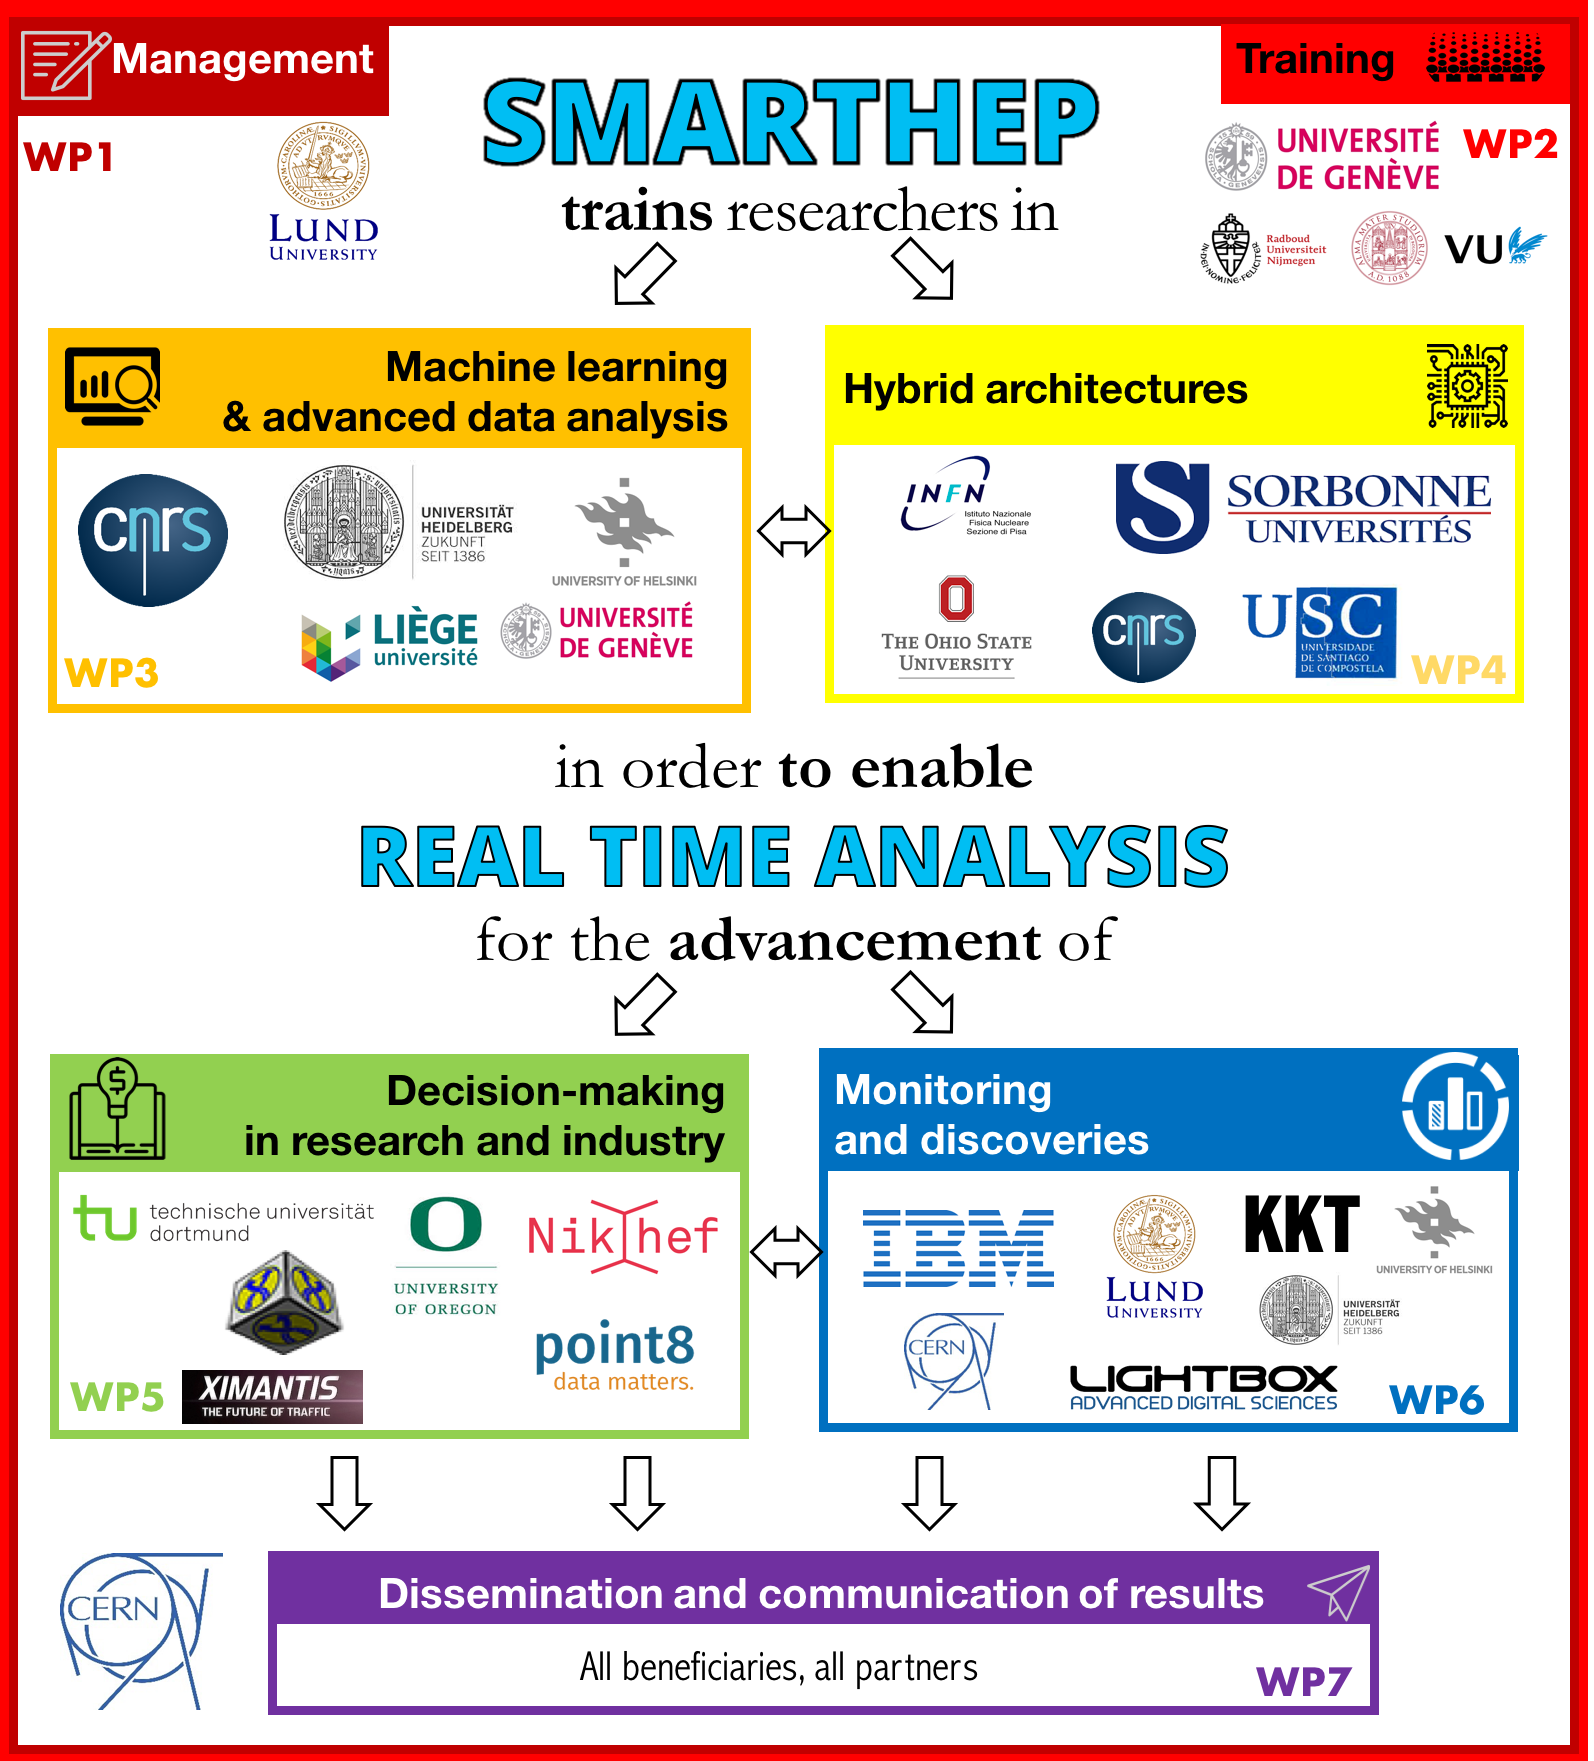
\includegraphics[width=0.9\textwidth]{figs/NetworkCompositionCombinedImplementation.png} %scienceStructure_2.pdf}
%%    \vspace{-8mm} 
%\caption{\acronym implementation strategy and main node expertise.}%\label{fig:implementation}}
%\label{fig:scienceStructure}
%%    \vspace{-3mm} 
%\end{figure}
%\clearpage

%{\color{blue}{Network topics and objectives}.}
\vskip2pt
\noindent{\color{blue}{Topics and research objectives}.} 
We define four main topics for \acronym,
focused on taking efficient decisions using RTA. 
All research topics require collaboration between industry and HEP, 
and have concrete outcomes beyond the state of the art benefiting both, only achievable with this network. 
The \acronym topics, goals and research objectives are:

%\vspace{-2mm}
%\begin{multicols}{2}[]
%%\small
\begin{enumerate}%{\leftmargin=1em}

\item\textbf{Machine learning and data analysis} Use Machine Learning as an enabling technology for real-time data analysis;
\begin{itemize}
\item Study of Machine Learning and Multivariate techniques (MVA), leading to HEP and commercial software toolkits; 
\item Implementation of efficient real-time object and event reconstruction, leading to software for the HEP experiments;
\item Benchmarking and optimization of algorithms, leading to inter-experiment toolkits. 
\end{itemize}

\item\textbf{Hybrid architectures} Design innovative solutions in hardware/software architectures for fast, efficient data analysis;
\begin{itemize}
\item Use of Field Programmable Gate Arrays, leading to a more efficient tracking for LHC experiments;%leading to a better for the ATLAS detector
\item Use of Graphic Processing Units, leading to significant speed-up for HEP RTA techniques;
\item Design of parallelized and multithreaded algorithms, leading to RTA software needed to face the increase in LHC data.
\end{itemize}

\item\textbf{Physics applications} Answer key physics questions through the analysis of LHC data with RTA;
\begin{itemize}
\item Discoveries in the Higgs and Dark Matter sectors, leading to results that probe unexplored ground;
\item Study of lepton flavor universality and violation, leading to possible confirmation of hints of physics beyond the SM;
\item High precision measurements of the Standard Model, leading to the most precise results on heavy ion physics to date;
\end{itemize}

\item\textbf{Industrial applications} Apply RTA techniques in the commercial sector.
\begin{itemize}
\item Applications towards a more efficient automotive transport, leading to software improvements for fleet control and traffic prediction;
\item Design and programming of sensors for Internet-of-Things, medical, process and computing optimization, leading to contributions to existing software and new toolkits. 
\end{itemize}

\end{enumerate} 
%\end{multicols}
%\vspace{-2mm}
%\vskip 5mm

%The connections between the consortium expertise, the different work packages
%and the overall \acronym strategy are shown in 
%Fig.~\ref{fig:scienceStructure}. 

The research objectives defined in \acronym go beyond the present state-of-the-art. 
They can only be achieved through the constitution 
of a multidisciplinary team, 
%shown in Fig.~\ref{fig:scienceStructure}
providing
the required research resources and the appropriate \textbf{training}. 
%Therefore, outstanding training will be an objective in itself.
%How the individual projects of the recruited researchers will be integrated into -- and contribute to
%-- the overall research program is described in more detail together with the research methodology in Sec.~\ref{sec:metho}.  
The concrete outcomes of \acronym will be \textbf{whitepapers, peer-reviewed publications and 
software toolkits} for the research objectives, that would not be possible without the expertise in this network. 
We also believe that the experience gained
with \acronym will lead to new interdisciplinary training models for scientists
in other data-intensive domains. With four in ten companies reporting a shortage of analytical skills\footnote{\href{http://www.forbes.com/sites/gilpress/2015/04/30/the-supply-and-demand-of-data-scientists-what-the-surveys-say/}{Supply and demand of data scientists}, Forbes 2015},
we believe that the proposed training program will increase the growth and competitiveness of 
European research, both in the academic and industrial sectors, while placing the foundations for a balanced career 
development model.

% that is becoming necessary.
% for research and industry to both contribute to European growth and competitiveness.

%Each of these topics has two aspects: first,
%the development of novel algorithms, analysis techniques and architecture designs,
%as defined in the ESR projects contributing to the research objectives; second,
%the implementation and documentation of these
%algorithms and techniques in a series of publications and software
%packages which will be accessible beyond the
%specific research projects of \acronym and will form its legacy.  


%Academic examples beyond \acronym include social sciences, astrophysics
%and cosmology, Earth sciences and climatology. 

%\acronym has two applications of IoT: 
%ESR3 will focus on a specific type of production chain with the goal
%of improving real-time data analysis and forecast by means of machine
%learning (ML) techniques. ESR7 will also, as secondment at
%WildTreeTech, use similar techniques to consult companies to exploit
%the data collected by their sensors. 
%Due to their architecture, the sensors can produce
%errors, therefore the raw data must be first corrected (filtered
%out). The real-time error correction and data analysis must be
%performed directly on the corresponding microcontrollers or
%single-board computers and due to their limited computational power
%should be highly optimized. 
% The data acquired in real-time by the connected sensors are of
% different nature, unstructured and complex, such as: parts vibration
% data, lubricant and fuel quality, wear particle data, temperature
% measurements, ultrasonic noise detection and flow, infrared
% thermorgraphy, electrical monitoring, etc. These data need to be
% collected, cleaned, aggregated and analyzed in real-time using both
% complex event processing infrastructure and statistical analysis
% techniques.

%%\paragraph{Text from Lightbox, to be reduced to a couple of sentences}
%\textbf{Internet of Things (IoT)} refers to the use of sensors and other
%Internet-connected devices to track and control physical objects
%through the industrial production chain and their subsequent end-user
%delivery steps. 
%In particular the deployment of sensors and systems that are connected
%and can exchange information allows companies to acquire real-time
%information of the operational status of each critical component in an
%industrial production chain. 
%Through IoT, companies may monitor the machine status and performance
%continuously and schedule maintenance only when necessary. 
%
%The combination of real-time and historical measurements data is used
%to infer when the production chain is getting close to a critical
%status that may require actions and to predict when a specific part of
%a machine will have to be fixed or replaced. The adoption of these
%techniques, called 

% Given the heterogeneity of the sensor data,
% ML techniques are beneficial in forecasting when machinery parts need
% intervention or should be replaced. 
%\vspace{1cm}

%\paragraph{Text from Cathi, is reduced, to be placed}
%CATHIS simulator is an interactive system based on software- and
%hardware-modules that provide realistic behaviour (visual and haptic)
%of medical instruments during the training process. 
%The core of the hardware modules is a set of sensors that generate different types of
%raw data (movement, pressure, reaction forces etc.) that must be
%analyzed in real-time and transferred to the software modules for
%further processing. The real-time error correction and data analysis must be
%performed directly on the corresponding microcontrollers or
%single-board computers and due to their limited computational power
%should be 
%highly optimized to fit the limited ressources.

\subsubsection{Research methodology and approach.}
\label{sec:metho}

\acronym defines four research WPs in the Table below and Fig.2, 
each corresponding to a research topic with its specific research objectives. 
The following table describes the motivations for each of the \acronym research topics and WPs and related ESRs. 
Additionally, WPs are defined for the management of the consortium, for training, and for outreach and dissemination.  
A description of the overall tasks for all WPs can be found in Sec.~\ref{sec:WPdescription}. 

\vskip10pt
\begin{center}
\scriptsize
\resizebox {\textwidth }{!}{%
%\begin{tabular}{@{}p{5mm}p{40mm}p{25mm}p{22mm}p{22mm}p{12mm}p{12mm}p{12mm}}
\begin{tabular}{p{7mm}p{30mm}p{35mm}p{5mm}p{5mm}p{35mm}p{17mm}p{17mm}}
%\begin{tabular}{l|l|l|l|l|l|l|l|}
\toprule
\pbox{8cm}{WP No.} &
\pbox{8cm}{WP Title} &
%This is the number of the beneficiary in the original order
\pbox{8cm}{\Tstrut No. of lead\\Beneficiary\Bstrut} &   
\pbox{8cm}{Start\\Month} &  
\pbox{8cm}{End\\Month} & 
\pbox{8cm}{Activity Type} & 
\pbox{8cm}{\Tstrut Lead Beneficiary\\Short Name\Bstrut} &  
\pbox{8cm}{ESRs\\Involvem't}\tabularnewline\toprule

\cellcolor{red!70!black} \textbf{\color{white}WP1\color{black}}  & Management & Doglioni  & 1 & 48 & Management & \lundentity & - \tabularnewline\hline\midrule

\cellcolor{red} \textbf{\color{white}WP2\color{black}}    & Training   & Sfyrla  & 5 & 42 & Recruitment and training & \unigeentity & All \tabularnewline\hline\midrule

\cellcolor{orange} \textbf{\color{black}WP3\color{black}}   & Data analysis and ML & Gligorov & 1 & 48 & Research& \cnrs & All \tabularnewline \hline%: Software and algorithms enabling RTA
\multicolumn{8}{p{\textwidth}}{\textbf{Motivation:} In order to optimize real-time analyses and selections,
it is important to employ the most powerful selection algorithms. One of the ML specialties is to find interesting features 
of data without being explicitly told what to look for. 
%This goal is achieved by minimizing some measure of error in predictions the machine learning algorithm makes. 
%In general, this is an iterative process in which the prediction is altered and the measure of error
%in prediction reevaluated in turn, lowering the total error. 
%The ability to go through a large amount of data and learn non-linear relations between the input
%variables 
This leads to remarkable performance in tasks of regression and classification.
The ability to learn from the analyzed datasets also makes ML a very attractive tool towards RTA applications.
%for fast and efficient data analysis
%, since once a decision is made then the data is lost.
Different ML algorithms are investigated by ESRs 1-3, 6, 9 for object reconstruction and feature identification, 
and for benchmarking and optimisation purposes for ESRs 4, 5, 7, 8, 10-12. 
Custom algorithms for real-time object reconstruction will be deployed by ESRs 3-5, 7, 14, 15.} \tabularnewline \hline \midrule
\cellcolor{yellow} \textbf{\color{black}WP4\color{black}}    & Hybrid architectures & Lacassagne & 1 & 48 & Research & \sorbonneentity  & 3, 4, 8, 9, 11, 15 \tabularnewline \hline % : Novel hardware for detectors and computing 
\multicolumn{8}{p{\textwidth}}{
\textbf{Motivation:} 
Innovative solution in hybrid hardware/software architectures are needed 
for faster, more efficient real-time data analysis, as the complexity and rate 
of the LHC data does not allow standard processors or data analysis techniques 
to be competitive (see J.P. Vlimant, \href{https://erez.weizmann.ac.il/pls/htmldb/f?p=101:58:::NO:RP:P58_CODE,P58_FILE:5393,Y}{Machine Learning in Charged Particle Tracking}, Hammers and Nails ML\&HEP Conference, 2017). 
The implementation of ML and detector reconstruction algorithms will be tested on GPUs by ESRs 3, 9, 10 and 11. 
Another example of a solution that ESRs 4, 8 and 15 will focus on is the ATLAS Fast TracKer (FTK)
(see ATLAS Collaboration,\href{https://inspirehep.net/record/1614024/}{The ATLAS Fast TracKer}, CERN Document Server, 2016), a unique hardware processor to reconstruct
the trajectory (track) of the charged particles that cross the inner part
of the experiment. The FTK is a complex system made by several
custom electronics boards based on FPGAs and unique computing devices.  %Associative Memory Chips
%The hardware tracking will be also a central part of the Phase-II Upgrade of ATLAS, with upgraded version of FTK called FTK+
%The tracking information is an essential tool for effective real-time event selection and has a
%central role in the whole ATLAS physics program especially in the HL-LHC phase. 
Moreover, with the end of Moore's law and the increase in parallelization and diversification of computing
architectures, it becomes increasingly complicated to design the optimal architecture for a processing task. 
Particularly for complex tasks, such as the real-time data processing of LHC experiments, there may be many
constraints involved: the I/O limitations of each architecture,
the memory limitations and compilers used, the optimal scheduling of subprocesses within each task. 
ESR10 will optimize data formats and processing techniques to enable CPUs, GPUs, FPGAs, 
and hybrids to work together to solve problems which none of these technologies could solve on their own, 
and as ESR4 and ESR8 will investigate parallelization and multithreading of current algorithms.
} \tabularnewline \hline \midrule

\cellcolor{lime} \textbf{\color{black}WP5\color{black}}   & Physics applications & Christiansen, Dunford, Voutilainen, Albrecht  & 1 & 48 & Research & \helsinkientity & 1-8, 10-15 \tabularnewline\hline %: Physics measurements and searches
\multicolumn{8}{p{\textwidth}}{
\textbf{Motivation:} 
The theory describing the Standard Model (SM) is incomplete. 
%%DM
Physics phenomena beyond the SM are needed to explain, for example, 
as observed from indirect gravitational and cosmological observations
the existence of massive "dark" matter present within our universe in amounts by far exceeding normal matter.%, or 
%%New Higgs searches
%the apparent difference between the measured mass of the recently discovered Higgs boson 
%and what theorized within the SM. %% PS I just removed the clause with Higgs mass, as it is dodgy
ESRs 1-4, 8, 13 and 15 search for new phenomena 
that could resolve these issues, and measure the properties of the Higgs boson. 
%%LFU
Precise measurements of the SM parameters can also highlight shortcomings
of the current theory. In particular, ESRs 5-7 and 10-12 probe the SM prediction 
that the weak force couplings to all lepton types are equal (Lepton Flavor
Universality, or LFU), and that the overall number of leptons of a given type
does not change in interactions (Lepton Flavor Violation, LFV). 
Recent measurements published by LHCb indicate that in 
%loop-level 
decays of beauty mesons, LFU might be
violated (see e.g. Phys. Rev. Lett. 113(2014)151601 and JHEP08(2017)055), 
%(CITE RK,RK*), 
making this one of the most interesting topics for the near-future of particle physics. 
%Two researches in this proposal are leading
%ERC research groups to further investigate this question. 
%CD this is best in the quality of the supervision
%%ALICE
The collective behavior of particles measured by ESR15 sheds light
on the state of matter present in the early universe 
a few milliseconds after the Big Bang. 
The common denominator of all those
searches and measurements is that they would not be possible without
specifically designed data taking techniques with a strong real-time component.
%as detailed in Sec.~\ref{sub:Originality}. 
%\vspace{-2mm}
} \tabularnewline \hline\midrule
%

%To split in 2 tables
%\bottomrule
%%\caption{Work-Package list.}\label{tab:WP}
%\end{tabular}
%}%end of resizebox
%\end{center}
%
%\vskip10pt
%\begin{center}
%\scriptsize
%\resizebox {\textwidth }{!}{%
%%\begin{tabular}{@{}p{5mm}p{40mm}p{25mm}p{22mm}p{22mm}p{12mm}p{12mm}p{12mm}}
%\begin{tabular}{p{7mm}p{30mm}p{35mm}p{5mm}p{5mm}p{35mm}p{17mm}p{17mm}}
%%\begin{tabular}{l|l|l|l|l|l|l|l|}
%\toprule
%\pbox{8cm}{WP No.} &
%\pbox{8cm}{WP Title} &
%%This is the number of the beneficiary in the original order
%\pbox{8cm}{\Tstrut No. of lead\\Beneficiary\Bstrut} &   
%\pbox{8cm}{Start\\Month} &  
%\pbox{8cm}{End\\Month} & 
%\pbox{8cm}{Activity Type} & 
%\pbox{8cm}{\Tstrut Lead Beneficiary\\Short Name\Bstrut} &  
%\pbox{8cm}{ESRs\\Involvem't}\tabularnewline\toprule
%
%%
\cellcolor{green} \textbf{\color{black}WP6\color{black}}   & Industrial applications & Meric, Starovoitov  & 1 & 48 & Research& \dqentity, \heidelbergentity & 1-4, 7-9, 11, 13, 15 \tabularnewline\hline %: Exploitation of RTA 
\multicolumn{8}{p{\textwidth}}{
\textbf{Motivation:} 
Real-time analysis techniques are employed in a variety of industrial contexts. \acronym
selected the cases with the best fit to the physics research program and techniques employed 
by each ESRs for their industrial secondments. Most ESRs include a project with
concrete industrial deliverables, concerning real-time traffic prediction (ESR1), in-vehicle mobile pattern recognition (ESR2), 
Internet-of-Things sensors (ESR3, ESR13, ESR15), 
task optimization and parallelization (ESR4, ESR8), 
efficient handling of computing clusters (ESR7), medical applications and insurance (ESR9, ESR11).
} \tabularnewline \hline\midrule
%

\cellcolor{cyan} \textbf{\color{black}WP7\color{black}}  & Dissemination, outreach  & Petersen & 1 & 48 & \pbox{8cm}{Dissemination and outreach} & \cern & All \tabularnewline
\bottomrule
%\caption{Work-Package list.}\label{tab:WP}
\end{tabular}
}%end of resizebox
\end{center}
%\vspace{-5mm}
%\end{table}
%\FloatBarrier
%\vspace{-5mm}
%{\color{blue}{Involvement of ESRs in WP and ROs}.}

%\textbf{\acronym answers the question: how do we build detectors which learn from their own performance
%and configure themselves to achieve an optimal understanding of the data which they collect, with as few human assumptions
%as possible, and within the constraints of real-time data processing?} 

Cutting-edge techniques in ML and hybrid architectures will be assessed and developed by the ESRs 
before their application to specific use cases, in order to enable RTA that advance HEP, industry and society, 
to follow with exploitation and dissemination (Sec.~\ref{sec:qualityExploitDissemination}), as shown in Fig.1. 
This modus operandi is at the heart of \acronym and ensures the efficiency of its implementation. 
Our research methodology seeks to apply RTA to novel problems posed by HEP;
in turn, the methods employed will evolve from exposure to these new challenges and
will be applied to novel industrial and commercial problems.
%This methodology is made explicit in Fig. 1.%~\ref{fig:scienceStructure}. 

%Each ESR develops novel methods in light of HEP problems, and applying DS methods to commercial applications. 
%This ensures that ESRs will be fully immersed in both HEP, while, at the same time, 
%advancing the state of the art in industry. 
%, 
%figure below. 
%\begin{center}
%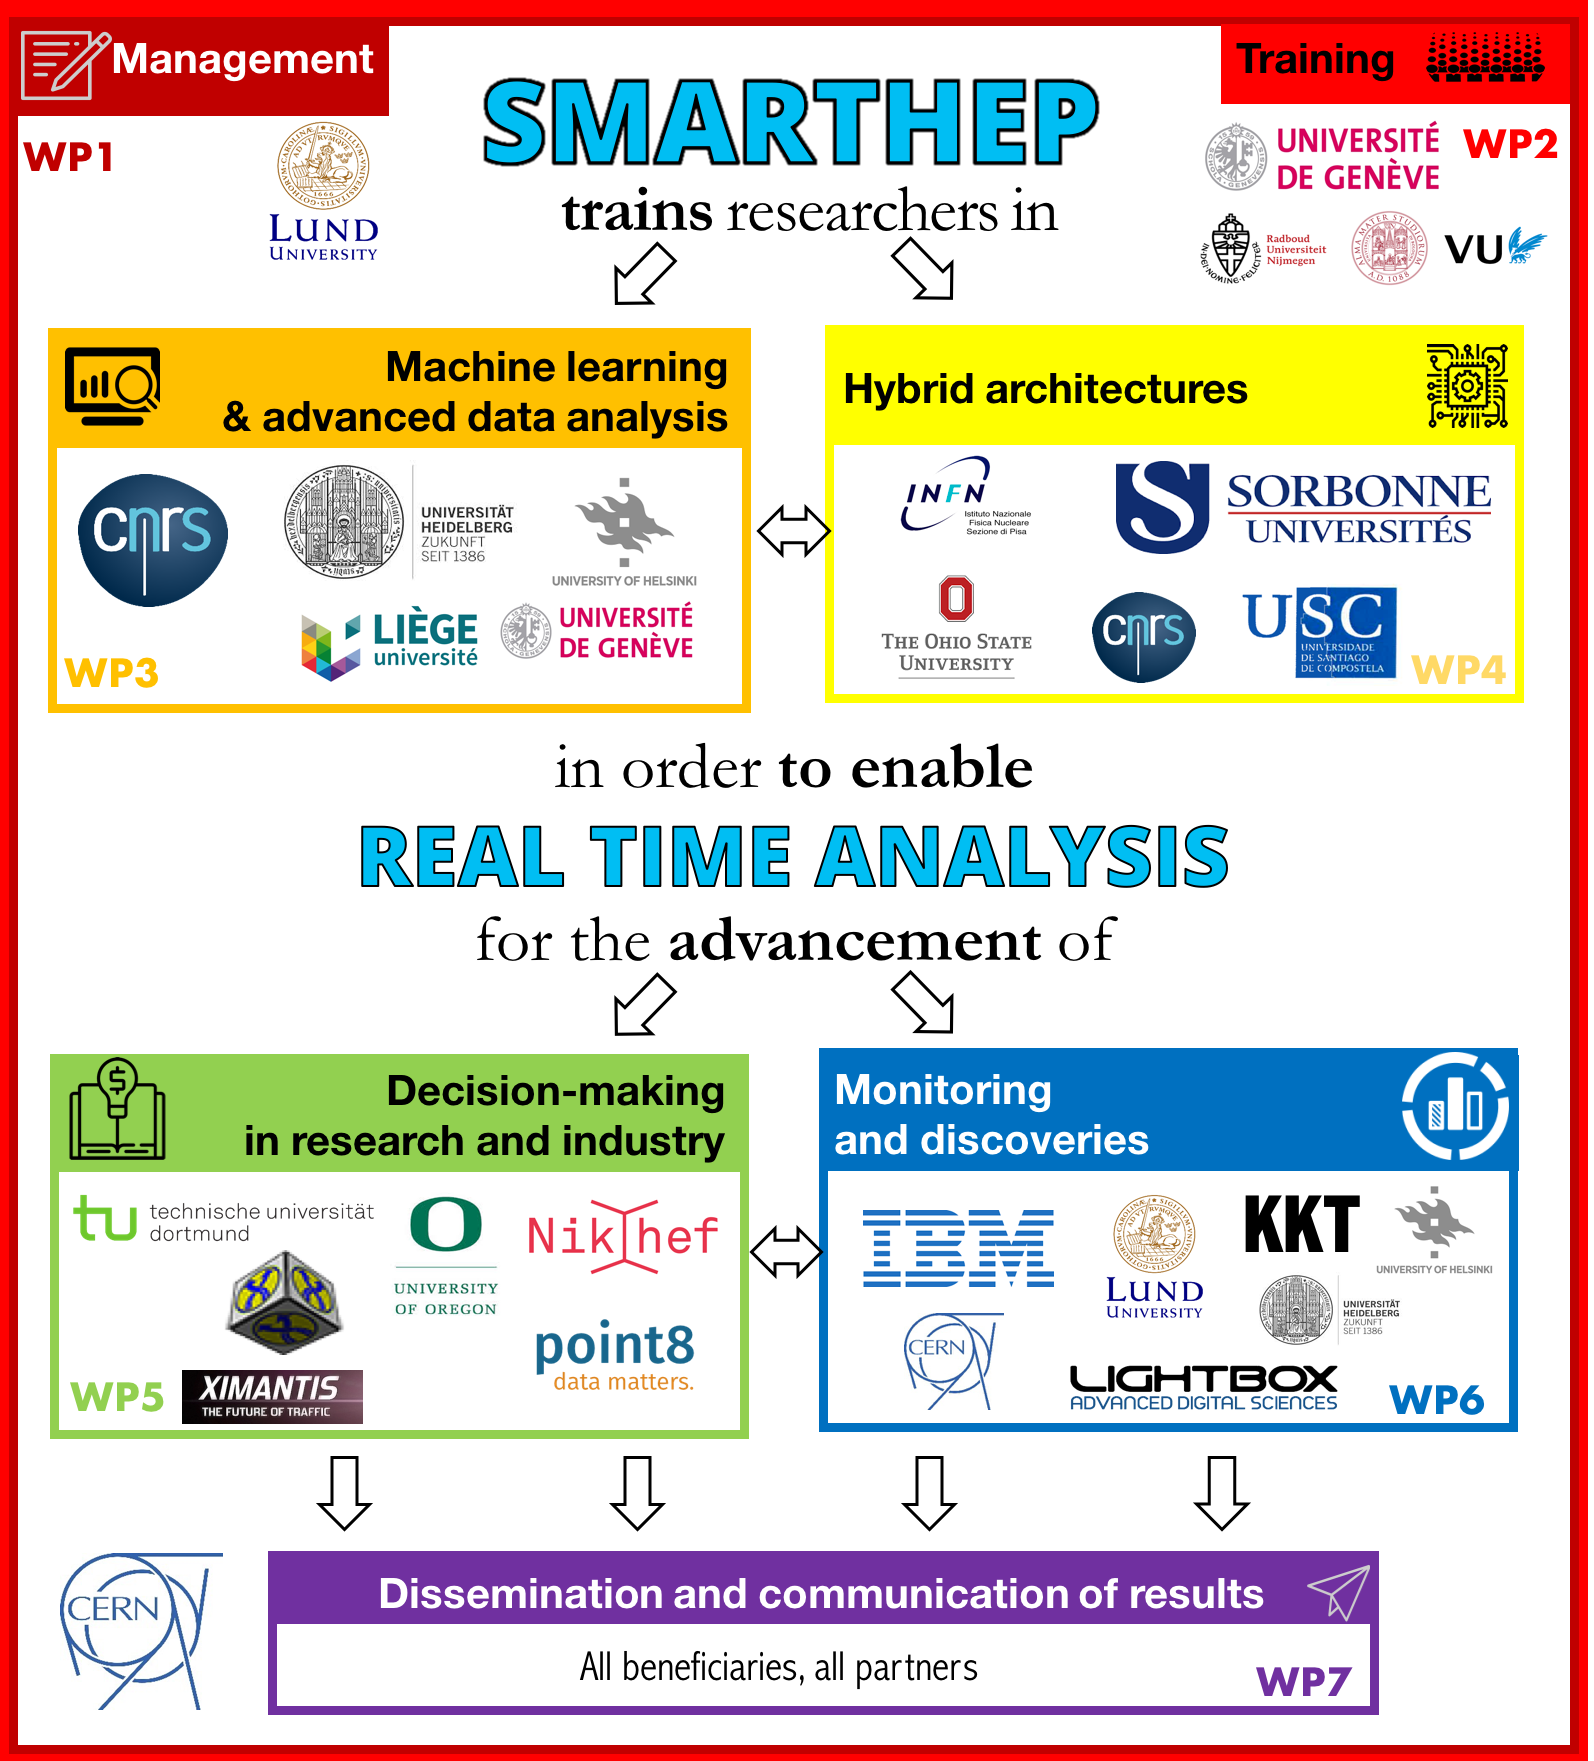
\includegraphics[width=0.75\textwidth]{figs/NetworkCompositionCombinedImplementation.png}\\ %scienceStructure_2.pdf}
%\end{center}

%This is in the figure now 
%%CD: I think a 2-column list here is unnecessary if you massage the endings of the sentences a bit, but you can change it back
%\vspace{-2mm}
%\begin{multicols}{2}[]
%\small
%\begin{enumerate}%{\leftmargin=1em}
%    \item Identify dataset to be studied, and key features/variables to be analyzed, clearly define intermediate milestones and research~path;
%    \item Research and master techniques to be applied to the dataset employed;
%    \item For commercial products, in collaboration with industrial partners: research market aspects and plan how to create value;
%    \item Implement identified techniques using appropriate computing infrastructures (local computing clusters, distributed LHC computing grid, hybrid architectures, etc.);
%    \item Present progress of each deliverable regularly within \acronym, group meetings, conferences. Actively seek feedback for improvement,
%     as described in Sec.~\ref{sub:progressMonitoring};
%    \item On completion, follow up on applications and external feedback on deliverables. 
%\end{enumerate} 
%\end{multicols}
%\vspace{-2mm}
%\vskip 5mm
%


%\vskip5pt
%and Network resources are shared to allow for their optimal completion.

%%%REPETITION ALARM: why do we have to have two tables? 

%(For ETN, it should be explained how the individual projects of the recruited researchers will be integrated into ? and contribute to 
% the overall research program. EJD and EID proposals should describe the research projects in the context of a doctoral training program)

%The action should be divided in Work Packages and described in the table below. The Work Packages should reflect the research objectives. Only brief headings and overviews of the Work Packages should be presented in Table 1.1. More details in terms of actual implementation should be provided in the tables under section 3.1.
 
%\FloatBarrier
%\begin{table}[!htb]
%\centering
\vspace{-2mm}
\subsubsection{Originality and innovative aspects of the research program} 
\label{sub:Originality}
%((in light of the current state of the art and existing programs / networks / doctoral research trainings)

HEP experiments are by their very nature built around \textbf{training}, 
as around a third of all LHC collaborations consist of PhD students.
This combination of a collaborative, training-based research culture, and a focus on the largest datasets
produced in the world using beyond state-of-the-art technology
leads to the proposal of \acronym as a training-centered research program in HEP and DS.
In the following, we cover the points that make the program of \acronym unique, 
in light of the current state of the art of research and doctoral trainings. 

%\begin{wrapfigure}{r}{0.75\textwidth}
%	\vspace{-5mm}
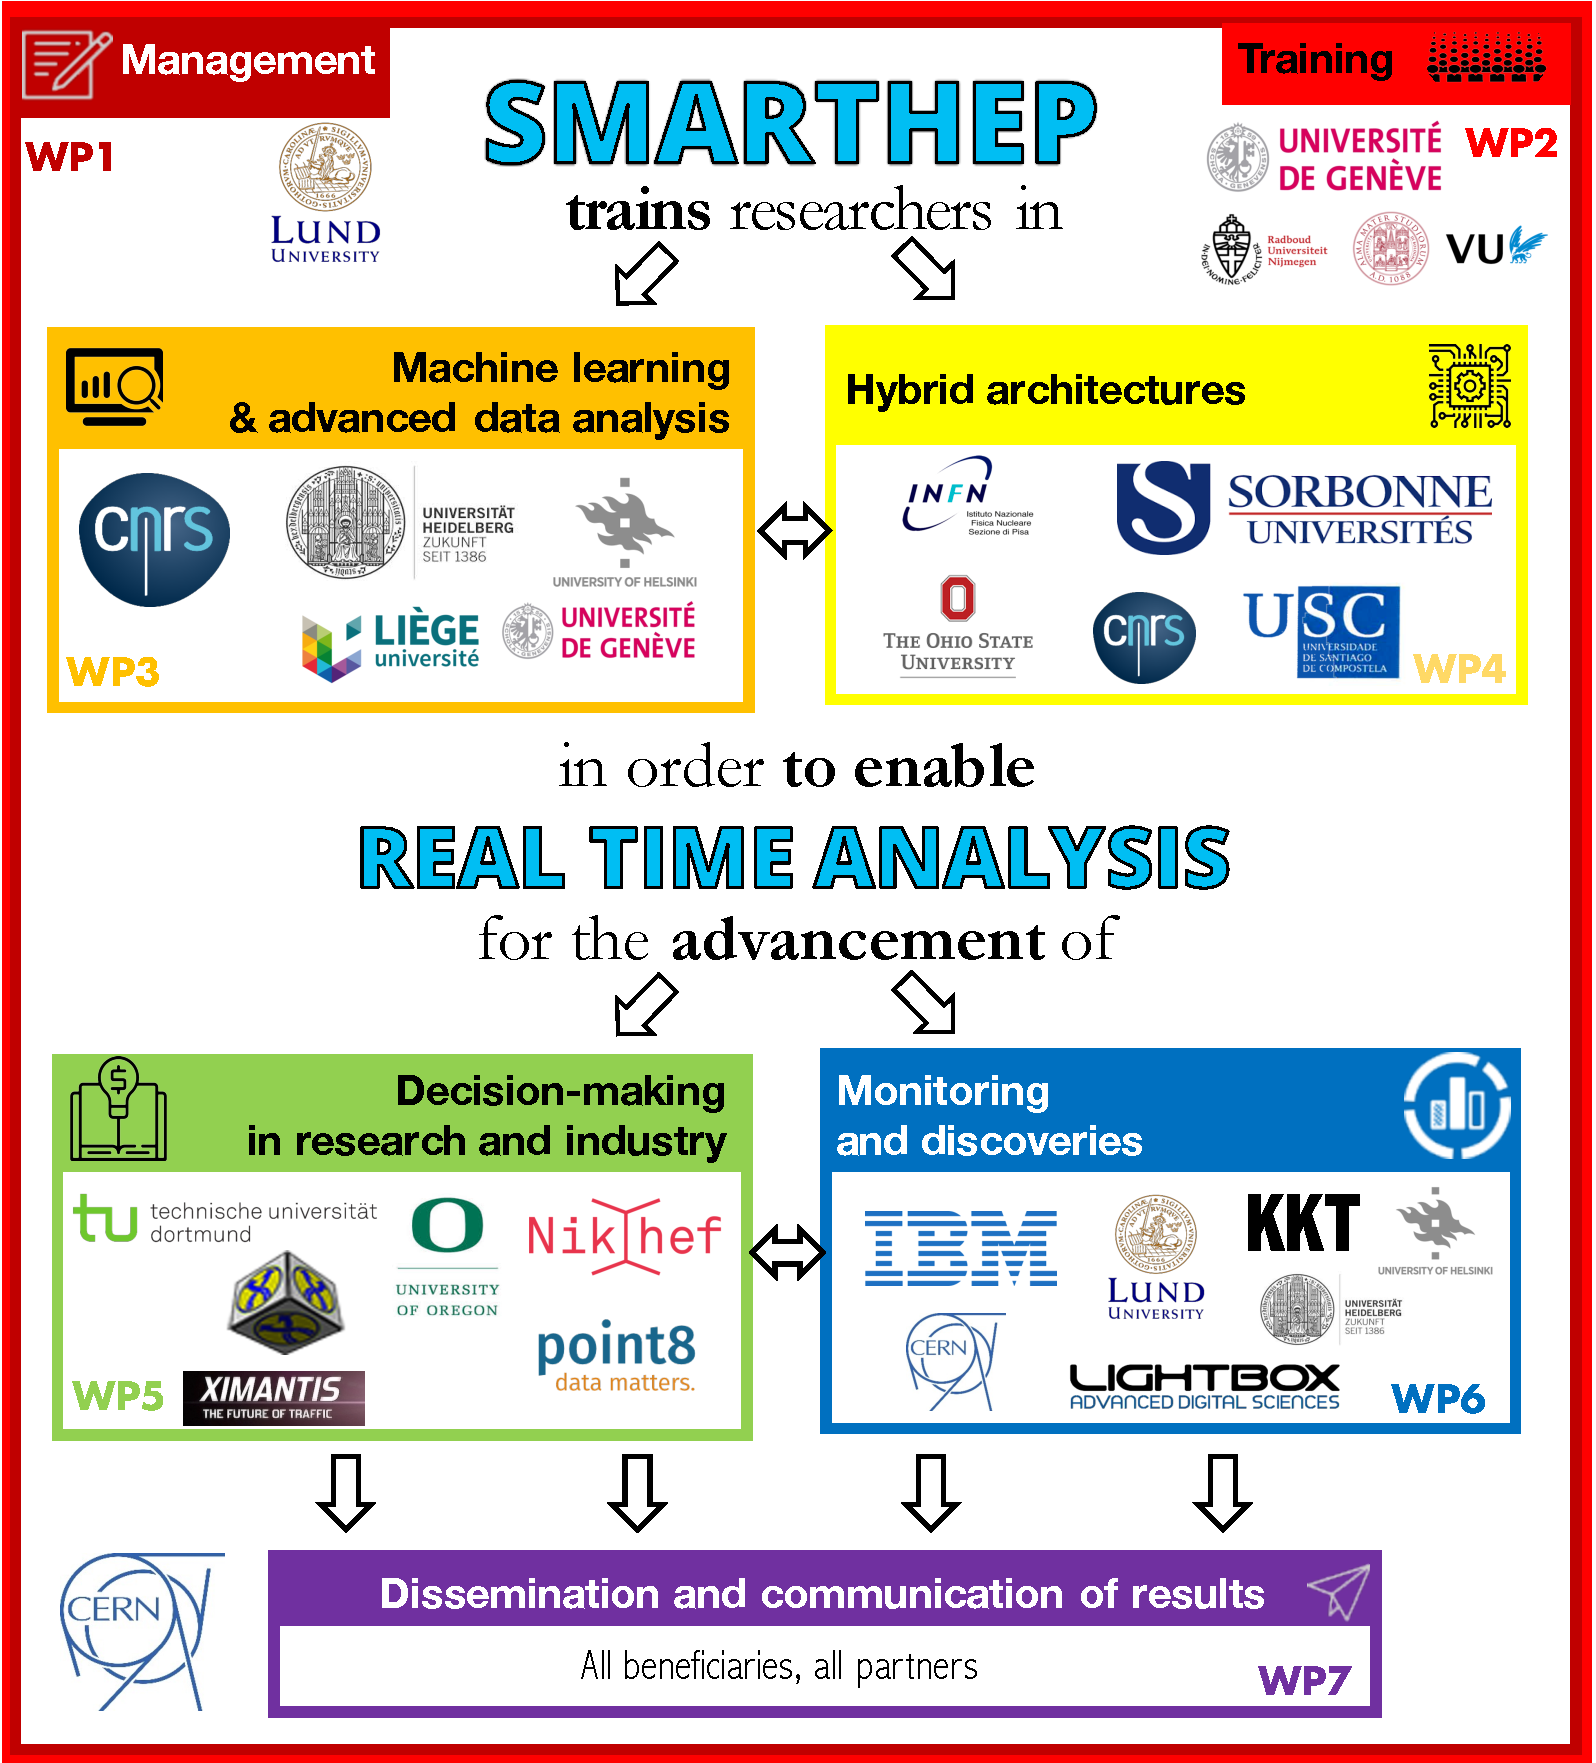
\includegraphics[width=\textwidth]{figs/NetworkCompositionCombinedImplementation} %scienceStructure_2.pdf}
    %\vspace{-8mm} 
%\label{fig:scienceStructure}
%    \vspace{-3mm} 
\begin{center}\footnotesize \label{fig:implementation}
Figure 1: \acronym implementation strategy and main node expertise.
\end{center}%\label{fig:implementation}}
\normalsize 
\vspace{-2mm}
 
\noindent {\color{blue}{1. Researchers from \acronym learn to systematically process large amounts of data with novel analysis techniques}.}
  \begin{wrapfigure}{r}{0.7\textwidth}
%%\begin{figure}{l}{\textwidth}
	%\vspace{12mm}
	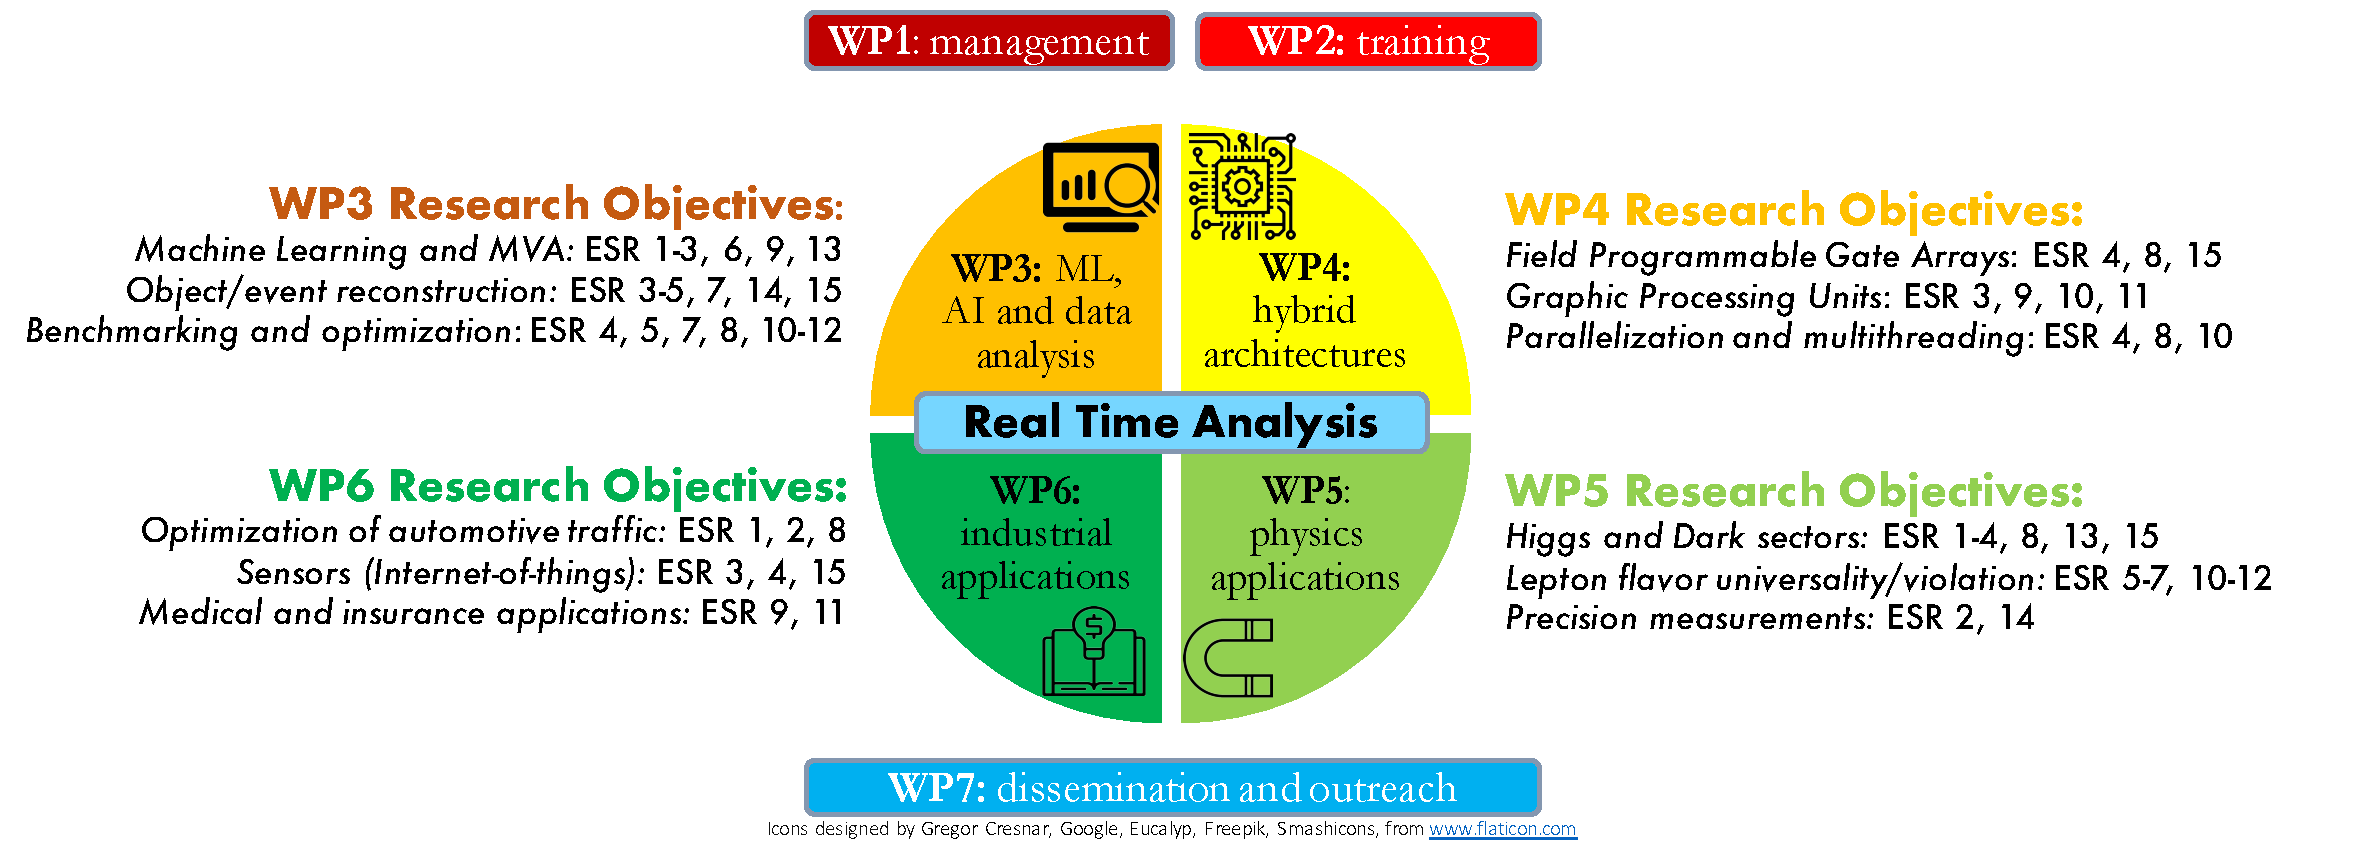
\includegraphics[width=0.7\textwidth]{figs/WPs} %scienceStructure_2.pdf}
%    \vspace{-5mm} 
	\caption*{Figure 2 : Structure and Research Objectives of the Work Packages.\label{fig:WPs}}
     %\vspace{-5mm} 
%%\begin{figure}	
\end{wrapfigure}
A large part of the novelty of this proposal is the volume of data which will
be processed, comparable to the largest commercial tasks. 
This is true across both academic and non-academic applications:
an estimated 90$\%$ of generated data is considered too expensive to store\footnote{\href{http://www.mckinsey.com/insights/business_technology/big_data_the_next_frontier_for_innovation}{2010 report on Big Data by McKinsey\&Company.}}.
One can compare Facebook and e.g. the LHCb collaboration:
the former processes hundreds of petabytes of data per year and spends half a billion
dollars a year on computing\footnote{Facebook, 
  \href{http://www.datacenterknowledge.com/the-facebook-data-center-faq-page-three/}{The Facebook Data Center FAQ}, 2010.}
while the latter processes thousands of petabytes of data per year
and spends around seven million dollars a year on computing\footnote{Private communication, \href{mailto:peter.clarke@ed.ac.uk}{Prof. Peter Clarke}, University of Edinburgh.}. The essential difference is that Facebook
stores and distributes this data to its users while LHC experiments 
largely process and then dispose of the data. An example of this are the physics searches and measurements performed
solely using trigger information. In these searches only a small fraction of each event, regardless of whether
LHC experiments are able to record it for offline reconstruction or not, is saved for further processing. 
This overcomes the storage limitations and allows to be more than an order of magnitude more sensitive
to certain new particles (e.g. associated to Dark Matter, as in Fig.3).

This requires a more systematic application of RTA, machine learning and 
hybrid architectures for HEP. 
E.g. for ML, ESR1 and ESR2 will make use of Deep Learning techniques,
which build high-level features from raw
data. ESR10 will use Recurrent Neural Networks (RNNs), which learn ordered patterns in the data and can be applicable both to tracking and to model paths taken by vehicles, and develop Generative Adversarial Networks (GAN), and ESR13 will implement anomaly detection techniques. 
This paradigm shift can be used in industry as well, 
while the research environment can benefit from a generation of
ESRs trained in industrial grade algorithms and tools. 

\begin{wrapfigure}{r}{0.4\textwidth}
	\vspace{-4mm}
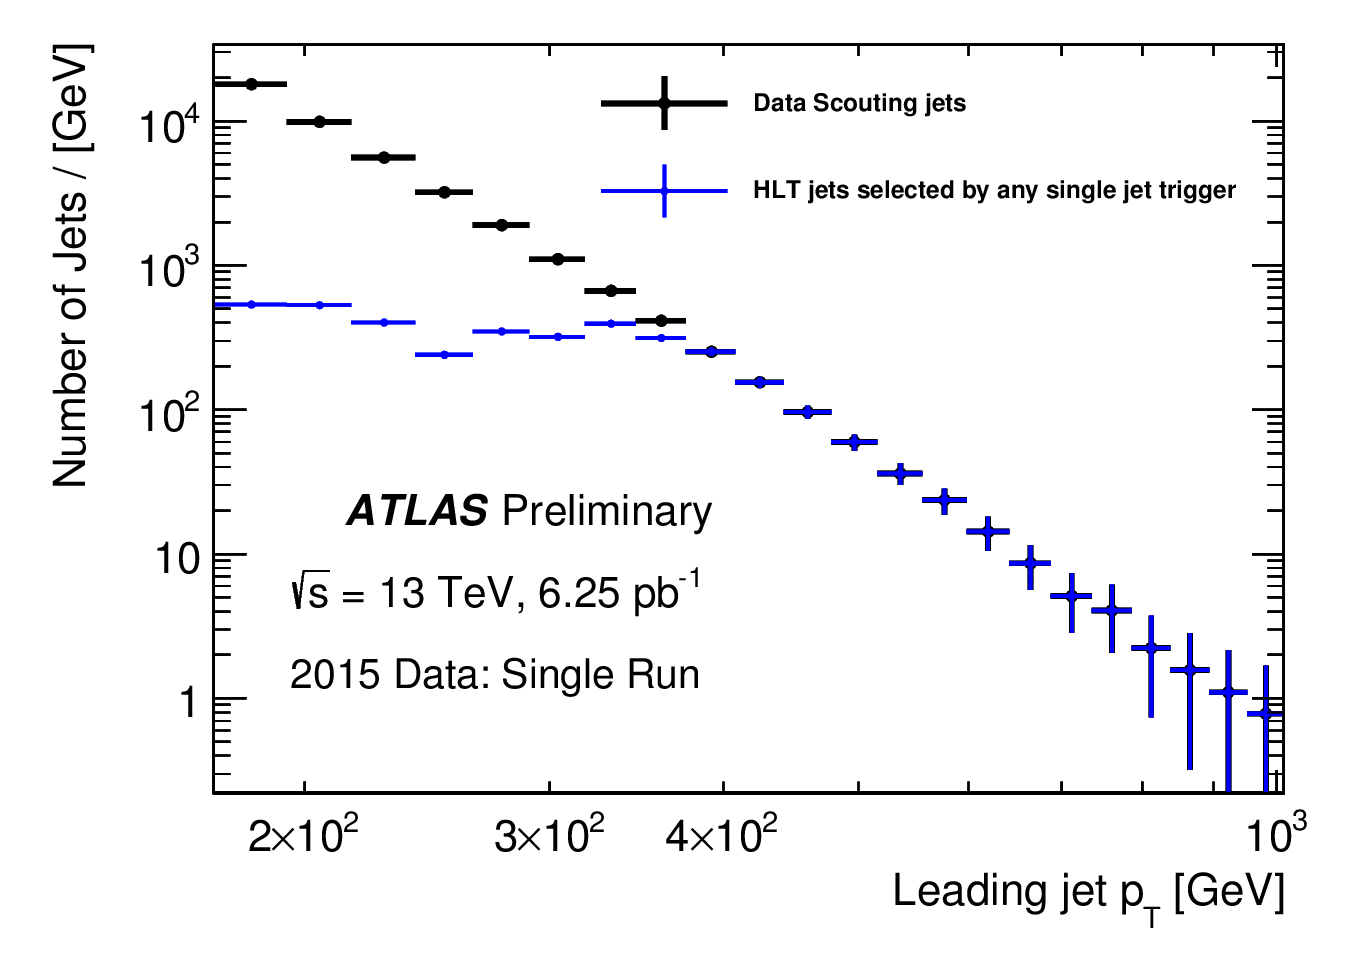
\includegraphics[width=0.4\textwidth]{figs/TLA.png} 
    \vspace{-10mm} 
    \caption*{Figure 3: Example of the number of events using traditional techniques (blue) compared to a trigger-level analysis (black)
in the search for new particles. Main analyzers: Boveia, Doglioni, Starovoitov, Dunford. \label{fig:TLA}}
\vspace{-4mm}
    \end{wrapfigure}
%    \vspace{-3mm} 
%Real-time analysis, machine learning and hybrid architectures have so far not been systematically
%applied to HEP problems. 
%Moreover, even where toolkits exist for HEP,
%notably \tmva\ or \scikit\, they are little more than a collection
%of individual algorithms applied in an ad-hoc manner.
%The research program of \acronym is developed coherently around 
%four main research questions that are at the forefront of 
%the long-term goals of all major LHC experiments. 
%which work against each other, 
%one generating examples and the other classifying them. 
%The classifying network gets a normal score, while 
%the generating network is scored when it can create an example	
%that escapes the classifier, so to make the classifier more 
%sensitive to non-standard cases as it is essential in RTA
%where rare, non-standard but interesting events risk being lost for good. 

%%CD: possible text about machine learning
%An additional driving challenge for the \acronym research program is the continuous need for improvement of background rejection
%techniques once the data has been taken. The discovery of the Higgs boson in 2012, which lead to the award of a Nobel Prize in Physics, has 
%opened the door to a whole new set of measurements of the properties of this new particle and possible discoveries 
%of deviations from the Standard Model. However, the frequency with which
%the Higgs boson particle is produced is minuscule compared to the rates of the backgrounds yielding the same detector signatures as the Higgs boson.  
%An efficient background rejection is key for both measurements involving the Higgs boson and similarly rare particles. 
%The need for novel techniques that only select the interesting events and reject the background is acute, in high energy physics and in
%commercial applications alike. The first challenge of analyzing events in real-time addressed by \acronym also has similar needs: 
%the current paradigm of triggering on simple features 
%ignores the growing importance of the analysis of raw, unstructured, data across both academia
%and industry. For both issues, a series of techniques known as machine learning, multivariate analysis, and 

\noindent {\color{blue}{2. The \acronym program of searches and measurement could
lead to breakthroughs in our understanding of nature}}
Research topics chosen to drive conceptual developments
within \acronym have potential to lead to 
the discovery of new physics beyond the standard model, but only RTA techniques enable
full exploitation of the LHC dataset. 
%the full statistical reach of the LHC data to be exploited. 
%Only RTA techniques will enable such discoveries. 
ESRs working on physics topics will target common challenges, e.g. 
when real-time algorithms and reconstruction techniques are not sufficiently 
advanced to distinguish signal from noise, 
or when the statistical power of the dataset is not fully
exploited if objects are reconstructed with traditional techniques. 
%The advanced tools under design in \acronym
%will allow the real-time systems of LHC 
%experiments to improve coherently. 

One central physics topic of \acronym is
lepton flavor physics. ESR 5-7, 9, 11-12 will work on questions concerning
the conservation and universality of lepton flavor in different final states and experiments,
as tantalizing hints of discrepancies between
measurements and SM theory have been recently reported. 
All measurements described here have the potential to be the most
sensitive by several orders of
magnitude. 
If existing hints for lepton non-universality turn out to be true, 
one would expect to see the first hints of lepton flavor violation in
some of these analyses. 
%CD: cut?
%ESR7 will work on novel real time selection strategies to extend the
%tests for LFU in semileptonically decaying decays of beauty mesons. 
%ESR5 and 11 will work on tests of LFV in tau decays,
%at the LHCb and ATLAS experiments, respectively. ESR9 will search for
%LFV in decays of mesons containing strange quarks and ESR 6 will
%examine the heavier charmonium and bottomonium systems.
Dark matter mediators and new light particles
are well-motivated new physics benchmarks\footnote{M. Chala et al,
\href{http://arxiv.org/abs/1503.05916}{Constraining Dark Sectors with Monojets and Dijets}, JHEP 1507 (2015) 089.}.
The volume of data needed to be sensitive to these rare processes is
the perfect testing ground for improved real-time techniques for ESR1 and 8.  
RTAs looking for dark matter mediators in ESR13 and 15, and the
search for new particles of ESR3 and 4 using ML
have never been performed at the LHC, 
nor have generic searches for rare new phenomena as in ESR2.
Measurements in ESR2 and 15 precisely probe the SM 
in the Higgs and heavy ions sectors. 

The choice of physics topics that all need RTA to achieve beyond-state-of-the-art results 
ensures advancement in detector development and contribution to
major advances in key analyses of LHC data.
%paving the way to understand the main questions of our universe. 

\noindent {\color{blue}{3. ESRs in \acronym deploy and disseminate their research at a unique time for particle physics}.}
As highlighted by the HEP Software Foundation Whitepaper$^{4}$,
the period 2019-2023 is ideal for this R\&D in HEP, as it
is a time of transition between LHC data taking periods that 
will be necessary to prepare for
an upgrade of the LHC accelerator where the amount of data delivered 
will make RTA techniques  the key to pursue 
the physics programs of the four main LHC experiments.
The systematic optimization of HEP experiments by \acronym
will boost the performance of the
current and planned upgrades of the CERN based accelerator
experiments. Furthermore, the developed toolkits will be advertised
at international conferences and thus the developed methods will
shape the online event selection of all future HEP experiments. 

\noindent {\color{blue}{4. \acronym researchers develop techniques and infrastructures that
can be exploited in industrial applications, as well as in HEP}.}
The close links of the research institutes of the consortium with the
industry partners means that the ESRs will directly drive the development of
novel industrial products, while also bringing professional methods
of data mining that are exercised in large
companies into the academic environment. 
Most modern methods applied in research can
in this way be transferred more easily to industry applications in automotive
traffic optimization (ESR1-2, 6, 8) 
%JA: not , 14 (??)) 
and analysis of sensor data for
Internet-of-Things and medical applications (ESR3-4, 9, 11, 13, 15).
The proposed algorithms and the use of machine learning methods on these
scales of data are novel to both HEP and industry. 
By exposing industry-grade methods to the volume and complexity of HEP data,
we will stimulate their development in a complementary way for the benefit of industry.

%\noindent {\color{blue}{5. \acronym researchers share information and write sustainable code}.}
%As the \acronym WPs intimately depend on each other,
%we will make the sharing of information, methods, and data between ESRs a centrepiece
%of our research strategy. Dedicated computing resources will
%be provided by the LHCb and ATLAS CERN groups for \acronym, and all ESRs will
%be required to 
%maintain and develop their research within this space
%accessible to the whole network. ESRs will be trained in
%maintaining digital logbooks\footnote{For example on \href{https://github.com}%{https://github.com} and using \href{https://jupyter.org}{Jupyter}.}%
%and documentation %so that other members of the network can profit from it, and 
%to ensure that
%they develop \textbf{sustainable} software, reusable both by
%other \acronym ESRs and later by others in
%the community. 
%Developing \textbf{sustainable software} is commonplace in industry but novel
%in physics, where the state of the art is usually a repository with notes about individual commits
%and a Doxygen server giving a web-based overview of the classes in the software. 
%By training the ESRs in state of the art industrial development methods, \acronym will also make a significant
%step forward in the development of physics software.
%Sustainability will encompass both the design (language, definition
%of interfaces and objects) of the software as well
%its documentation (writing individual methods a non-expert can read,
%comment cards in the source code, external documentation explaining algorithms and program flow).
%All developed methods and code will be shared; however, the data of the ALICE, CMS, LHCb and %ATLAS experiments will be treated according to the regulations of the
%respective collaborations. %The collaborative approach which is mandated by
%the described interdependency of the different aspects of our research program is at the heart of our research methodology.


%\end{document}

%flush all figs and tables up to here, but keep them at the end
\processdelayedfloats

{\scriptsize \noindent \color{red} YR SUGGESTED PAGE COUNT - KEEP TO 7-8+\numberofextrapages PAGES UP TO HERE \\
\noindent \makebox[\linewidth]{\rule{\textwidth}{0.4pt}}\normalsize }

%%%Commented out to update to 2018
%%%1.2
\vspace{-2mm}
\subsection{Quality and innovative aspects of the training programme}
\label{sec:training}
%The training program of \acronym has three main {\bf objectives}, taking the Salzburg Principles\footnote{Salzburg II recommendations, \url{http://www.eua.be/Libraries/publications-homepage-list/Salzburg_II_Recommendations}} as a guidance: 
\begin{itemize}
\item {\bf Objective A}: provide ESRs with knowledge and training to conduct original research during and beyond their PhD studies;
\item {\bf Objective B}: provide solid bases in a broad spectrum of topics related to their field of research, extending beyond their dedicated research and including soft skills; 
\item {\bf Objective C}: provide up-to-date and career-related training through interactions with multiple collaborators within academia as well as the industry, to meet the needs of a broad employment market.
\end{itemize}

%MLD what does 'career-focused aspects' supposed to mean?
Objectives A and B will be fulfilled by schools, workshops and events organized within the network; ESRs will profit from high quality lectures delivered by experts within the institutes associated to \acronym, complemented by doctoral training at local nodes. Objective C will be fulfilled by mentoring by senior scientists and special network events where the industrial collaborators will provide seminars and training on commercial applications of \acronym's objectives. All these objectives will be further addressed via the natural collaboration between the ESRs and the various institutes of the network, as well as the planned secondments in academia and industry. This is a more flexible and diverse structure compared to standard PhD studies and will allow the ESRs to develop an individual and unique research mindset within an inclusive environment, so that they can act as proactive participants in furthering HEP and industry goals through RTA techniques.

\vspace{-2mm}
\subsubsection{Overview and content structure of the training}
\label{sub:overviewTraining}
%(including network-wide training events and complementarity with those programs offered locally at the participating organisations (please include table 1.2a and table 1.2b)

%MLD be consistent with the use of names, some times the responsible is named, other times not
Training is at the heart of all activities within \acronym, with a dedicated Work Package, WP2. ESRs will have clear recruitment deliverables, a Personal Career Development Plan (PCDP), and they will be able to attend complementary network-wide and local training accounted through a credit system designed for this ETN. The recruiting deliverables, the composition of the Supervisory Committee (SC) for each ESR and the expertise and qualification of supervisors is shown in Tab. 1.2.

\begin{center}\scriptsize
\begin{tabular}{|p{0.05\textwidth}|p{0.07\textwidth}|p{0.1\textwidth}|p{0.06\textwidth}|p{0.05\textwidth}|p{0.45\textwidth}|}
\hline
\pbox{8cm}{\textbf{ESR}} & 
\pbox{8cm}{\Tstrut \textbf{Recruiting} \\ \textbf{node} \Bstrut} &  
\pbox{8cm}{\Tstrut \textbf{PhD-awarding} \\ \textbf{node} \Bstrut} &  
\pbox{8cm}{\Tstrut \textbf{Planned} \\ \textbf{start} \Bstrut} &  
\pbox{8cm}{\Tstrut \textbf{Duration}} & 
\pbox{8cm}{\Tstrut \textbf{Title}} 
\tabularnewline 
\hline
%%%
%Only PhDs now
\textbf{\ESRa} & \helsinkientity & \helsinkientity & 8 & 36 & ML and RTA for Higgs boson measurements and industry \tabularnewline \hline  
\textbf{SC} & \multicolumn{5}{p{0.9\textwidth}|}{
\textbf{Main supervisor: Voutilainen} (\helsinkientity), [2]. Assistant prof. Expertise: RTA, SM and Higgs measurements, with positions of responsibility in CMS. Grant from the Finnish Academy of Science, prizes for research during PhD and postdoc. } \tabularnewline %[8/3/2] in particle physics (HEP)
 & \multicolumn{5}{p{0.9\textwidth}|}{\textbf{Second supervisor: Pierini} (\cernentity) [6]. Staff scientist. Expertise: RTA, ML for HEP. ERC CoG for ML at the LHC.}\tabularnewline %[Al momento ho 3 undegraduate, 1 graduate e 3 fellow In piu?, ogni anno prendo 5-10 intern (summer student e similar) e co-supervisiono studenti PhD in CMS (al momento due di Caltech)]
 & \multicolumn{5}{p{0.9\textwidth}|}{\textbf{Industrial supervisor: Taccari} (\fleetmaticsentity). Data scientist. Expertise: mathematical optimization and ML. }\tabularnewline 
 & \multicolumn{5}{p{0.9\textwidth}|}{\textbf{Supervising postdoc: Kirschenmann} (\helsinkientity). Expertise: LHC jet physics and searches, with positions of responsibility in CMS. } \tabularnewline
 & \multicolumn{5}{p{0.9\textwidth}|}{\textbf{Senior mentor: Eerola} (\cernentity). Professor (HEP), Vice Rector of the University of Helsinki.}\tabularnewline %[19]
  \hline \hline
%%%
%%%
\textbf{\ESRb} & \unigeentity & \unigeentity & 8 & 36 & ML pattern recognition for exotic physics and industry \tabularnewline \hline 
\textbf{SC} & \multicolumn{5}{p{0.9\textwidth}|}{
\textbf{Main supervisor: Sfyrla} (\unigeentity), [2]. Assistant prof. (HEP). Expertise: SUSY DM and trigger expert, responsibility positions in ATLAS in trigger and HL-LHC upgrade. Grant from the Swiss National Foundation.} \tabularnewline %[3/2]
 & \multicolumn{5}{p{0.9\textwidth}|}{\textbf{Second supervisor: Martinez-Santos} (\santiagoentity) [6]. Assistant prof. (HEP). Expertise: rare decays, trigger and detectors. ERC StG for BSM searches. }\tabularnewline 
 & \multicolumn{5}{p{0.9\textwidth}|}{\textbf{Industrial supervisor: Catastini} (\lightboxentity). Quantitative Analyst. Expertise: analysis of financial markets, automated digital advertising trading.}\tabularnewline 
 & \multicolumn{5}{p{0.9\textwidth}|}{\textbf{Supervising postdoc: Schramm} (\unigeentity). Expertise: ML and new physics, convener of LHC interexperiment ML group until 2018, Banting Fellow.} \tabularnewline
 & \multicolumn{5}{p{0.9\textwidth}|}{\textbf{Senior mentor: Iacobucci} (\unigeentity). Director of the DPNC at \unigeentity. }\tabularnewline \hline \hline
%%%
%%%
\textbf{\ESRc} & \cernentity & \unigeentity & 8 & 36 &Efficient RTA in ATLAS using multi-threaded processing \tabularnewline \hline 
\textbf{SC} & \multicolumn{5}{p{0.9\textwidth}|}{
\textbf{Main supervisors: Petersen}(\cernentity), [2]. Staff scientist. SUSY DM and trigger expert, past ATLAS trigger convener, current upgrade physics convener; \textbf{Sfyrla} (\unigeentity), see \ESRb }\tabularnewline %[8/3/2]
 & \multicolumn{5}{p{0.9\textwidth}|}{\textbf{Second supervisor: Crescioli} (\cnrsentity) [2]. Research engineer. FTK and FPGA expert, technical coordinator of many R\&D projects;}\tabularnewline 
 & \multicolumn{5}{p{0.9\textwidth}|}{\textbf{Industrial supervisor: Catastini} (\lightboxentity), see \ESRb. }\tabularnewline   
 & \multicolumn{5}{p{0.9\textwidth}|}{\textbf{Senior mentor: Monica Pepe-Altarelli} (\cernentity). Staff scientist. Vice-President Elected at Large of the Executive Council of \href{http://iupap.org/}{IUPAP}}\tabularnewline \hline \hline
 %& \multicolumn{5}{p{0.9\textwidth}|}{\textbf{Supervising postdoc: E (if available)} (place). Expertise: [Text]} \tabularnewline \hline \hline
%%%
%%%
\textbf{\ESRd} & \dortmundentity & \dortmundentity & 8 & 36 &Real-time ML for LFV in unflavoured meson decays \tabularnewline \hline %Eerola [19], 
\textbf{SC} & \multicolumn{5}{p{0.9\textwidth}|}{
\textbf{Main supervisor: Albrecht}(\dortmundentity), [8]. Assistant prof. and Emmy Noether group leader. Expertise: LFV/LFU, tracking, ML and trigger expert, deputy Physics Coordinator of LHCb. ERC StG 2016 on LFV/LFU.  } \tabularnewline %8/18
 & \multicolumn{5}{p{0.9\textwidth}|}{\textbf{Second supervisor: Martinez-Santos} (\santiagoentity [6], see \ESRb.}\tabularnewline 
 & \multicolumn{5}{p{0.9\textwidth}|}{\textbf{Industrial supervisor: Sopasakis} (\ximantisentity). Mathematics and ML/AI expert, CEO and \lundentity associate professor, start-up experience.}\tabularnewline 
 & \multicolumn{5}{p{0.9\textwidth}|}{\textbf{Supervising postdoc: Matev} (\cernentity). Expertise: software and trigger design and maintenance.} \tabularnewline 
 & \multicolumn{5}{p{0.9\textwidth}|}{\textbf{Senior mentor: Spaan} (\dortmundentity). Head of experimental physics 5, team leader for the LHCb experiment, project leader of CS research area SFB876.}\tabularnewline \hline \hline
%%%
%%%
\textbf{\ESRe} & \dortmundentity & \dortmundentity & 8 & 36 & Global event triggering in LHCb \tabularnewline \hline %Eerola [19], 
\textbf{SC} & \multicolumn{5}{p{0.9\textwidth}|}{
\textbf{Main supervisor: Albrecht}(\dortmundentity), [13]. Assistant prof. See \ESRd.} \tabularnewline
 & \multicolumn{5}{p{0.9\textwidth}|}{\textbf{Second supervisor: Raven} (\nikhefentity) [14]. Professor. expert in LFV/LFU and triggering in LHCb with positions of responsibility, receiver of several national grants. }\tabularnewline 
 & \multicolumn{5}{p{0.9\textwidth}|}{\textbf{Industrial supervisor: Dungs} (\pointeightentity). Staff. Expertise: transitioned from LHCb trigger group to data science (via Google). }\tabularnewline 
% & \multicolumn{5}{p{0.9\textwidth}|}{\textbf{Additional supervision: Pearce} (\cernentity). Expertise: [Text]} \tabularnewline \hline \hline
 & \multicolumn{5}{p{0.9\textwidth}|}{\textbf{Senior mentor: Spaan} (\dortmundentity), see \ESRd. }\tabularnewline \hline \hline
%%%
%%%
\textbf{\ESRf} & \cnrsentity & \sorbonneentity & 8 & 36 & Real-time trajectory reconstruction in ATLAS \tabularnewline \hline %Eerola [19], 
\textbf{SC} & \multicolumn{5}{p{0.9\textwidth}|}{
\textbf{Main supervisors: Crescioli} (\cnrsentity and \sorbonneentity), see \ESRc \newline
\textbf{Malaescu}(\cnrsentity and \sorbonneentity), [4], Assistant prof. Expertise: jet measurements and searches, ATLAS SM group convener, past Statistics Forum convener. 
}\tabularnewline 
 & \multicolumn{5}{p{0.9\textwidth}|}{\textbf{Second supervisor: Roda} (\pisaentity) [14]. Expert in searches beyond the SM, ATLAS Pisa group leader, coordination roles in ATLAS.}\tabularnewline 
 & \multicolumn{5}{p{0.9\textwidth}|}{\textbf{Industrial supervisor: Sambo} (\fleetmaticsentity). Senior Data Scientist. Expertise: AI, ML, connected vehicles. }\tabularnewline 
 & \multicolumn{5}{p{0.9\textwidth}|}{\textbf{Additional supervision: Annovi} (\pisaentity). Expertise: tracking and track triggers for ATLAS} \tabularnewline 
 & \multicolumn{5}{p{0.9\textwidth}|}{\textbf{Senior mentor: Calderini} (\cnrsentity), Team leader, AIDA2020 management. Expertise: detectors, SM in ATLAS}\tabularnewline \hline \hline
%%%
%%%
\textbf{\ESRg} & \sorbonneentity & \sorbonneentity & 8 & 36 & Real-time trajectory reconstruction in ATLAS \tabularnewline \hline %Eerola [19], 
\textbf{SC} & \multicolumn{5}{p{0.9\textwidth}|}{
\textbf{Main supervisor: Lacassagne} (\sorbonneentity), [15], Professor. Hybrid architectures expert, leader of LIP6 Hardware and Software for Embedded Systems team. }\tabularnewline 
 & \multicolumn{5}{p{0.9\textwidth}|}{\textbf{Second supervisor: Petersen}, see \ESRc }\tabularnewline 
 & \multicolumn{5}{p{0.9\textwidth}|}{\textbf{Industrial supervisor: Borri} (\lightboxentity). Staff. Expertise in quantitative analysis and automated financial market trading expert.}\tabularnewline 
 & \multicolumn{5}{p{0.9\textwidth}|}{\textbf{Additional supervision: Couturier} (\cernentity). Expertise: software architect for various companies, now core team of LHCb software framework} \tabularnewline \hline \hline
%%%
%%%
\textbf{\ESRj} & \ibmentity & \lundentity & 8 & 36 &Novelty detection for industry and ATLAS searches \tabularnewline \hline %Eerola [19], 
\textbf{SC} & \multicolumn{5}{p{0.9\textwidth}|}{
\textbf{Main supervisors:  Julli\'{e}} (\ibmentity), Software Engineer. Expertise: modelling optimization problems, ML, anomaly detection. \newline
\textbf{Doglioni} (\lundentity), [6], Assistant prof. Expertise: jet, trigger and Dark Sectors expert in ATLAS, LHC Dark Matter WG organizer and HSF trigger and reconstruction WG convenor, ERC StG 2015 on RTA for ATLAS, national grants. }\tabularnewline 
 & \multicolumn{5}{p{0.9\textwidth}|}{\textbf{Second supervisor: Boveia} (\ohioentity). Expertise: Dark Sectors, trigger and track trigger ATLAS, responsible for first fully RTA-based search in ATLAS. } \tabularnewline 
 & \multicolumn{5}{p{0.9\textwidth}|}{\textbf{Additional supervision: Shaw} (\ibmentity). Expertise: constraint programming, optimization modelling and local search.} \tabularnewline 
 & \multicolumn{5}{p{0.9\textwidth}|}{\textbf{Senior mentor: Akesson} (\lundentity). Professor. Expert in searches at ATLAS. Member of the Nobel Committee and ex-CERN Council president. }\tabularnewline \hline \hline
 
%%%
%%%
 \multicolumn{6}{p{0.95\textwidth}}{
\footnotesize 
\vskip2pt
Table 1.2: Recruitment deliverables per beneficiary, Supervisory Committee (SC) with number of supervised PhD students and postdocs, and expertise/qualification of supervisors. 
\vskip2pt
\normalsize
}
\end{tabular}
\end{center}

\newpage


\begin{center}\scriptsize
\begin{tabular}{|p{0.05\textwidth}|p{0.07\textwidth}|p{0.1\textwidth}|p{0.06\textwidth}|p{0.05\textwidth}|p{0.45\textwidth}|}
\hline
\pbox{8cm}{\textbf{ESR}} & 
\pbox{8cm}{\Tstrut \textbf{Recruiting} \\ \textbf{node} \Bstrut} &  
\pbox{8cm}{\Tstrut \textbf{PhD-awarding} \\ \textbf{node} \Bstrut} &  
\pbox{8cm}{\Tstrut \textbf{Planned} \\ \textbf{start} \Bstrut} &  
\pbox{8cm}{\Tstrut \textbf{Duration}} & 
\pbox{8cm}{\Tstrut \textbf{Title}} 
\tabularnewline 
\hline
%\ESRx & \ibmentity  & \ & 8 & 36 & \textit{Feillet}, Lacassagne [15/21] & Gligorov [3/2]  \tabularnewline \hline
\textbf{\ESRx} & \ibmentity & \sorbonneentity & 8 & 36 & Real-time rule induction in fraud detection and HEP \tabularnewline \hline %Eerola [19], 
\textbf{SC} & \multicolumn{5}{p{0.9\textwidth}|}{
\textbf{Main supervisor:  Feillet} (\ibmentity), [N],[Position]. Expertise: [Text]. [Qualifications and grants] \newline
\textbf{Lacassagne} (\sorbonneentity), [15], See \ESRg.}\tabularnewline 
 & \multicolumn{5}{p{0.9\textwidth}|}{\textbf{Second supervisor: Gligorov} (\cnrsentity) [3]. Staff scientist. Expertise: ML, LFV/LFU, trigger, past LHCb Deputy Physics Coordinator, Real-time analysis project coordinator. ERC CoG 2016 on RTA and LFV/LFU in LHCb. }\tabularnewline 
 & \multicolumn{5}{p{0.9\textwidth}|}{\textbf{Additional supervision: Louppe} (\liegesentity) [3]. Assistant prof. Expertise: artificial intelligent and deep learning, Analysis Consultant Expert with ATLAS. }\tabularnewline \hline \hline
% & \multicolumn{5}{p{0.9\textwidth}|}{\textbf{Additional supervision: Louppe} (place) [N]. [Position]. Expertise: [Text]. [Qualifications and grants] }\tabularnewline 
%%%
%%%
\textbf{\ESRk} & \lundentity & \lundentity & 8 & 36 &Real-time calibration and analysis of the ALICE Time Projection Chambers (TPC) \tabularnewline \hline %Eerola [19], 
\textbf{SC} & \multicolumn{5}{p{0.9\textwidth}|}{
\textbf{Main supervisor: Christiansen} (\lundentity), [17], Professor. Expertise: ALICE TPC, real-time detector reconstruction and analysis in ALICE, receiver of several national grants. }\tabularnewline 
 & \multicolumn{5}{p{0.9\textwidth}|}{\textbf{Second supervisor: Shahoyan} (\cernentity) [2]. Staff scientist. Expertise: expert in calibration and data analysis in ALICE, main developer of real-time reconstruction project. }\tabularnewline 
 & \multicolumn{5}{p{0.9\textwidth}|}{\textbf{Industrial supervisor: Sopasakis} (\ximantisentity). See \ESRd. }\tabularnewline \hline \hline
 %& \multicolumn{5}{p{0.9\textwidth}|}{\textbf{Additional supervision: Shahoyan} (\cernentity). Expertise: [Text]} \tabularnewline 
\hline \hline
%%%
%%%
\textbf{\ESRh} & \nikhefentity & \radboudentity & 8 & 36 &Optimization of RTA resources and ATLAS LFV search \tabularnewline \hline %Eerola [19], 
\textbf{SC} & \multicolumn{5}{p{0.9\textwidth}|}{
\textbf{Main supervisor: Igonkina} (\nikhefentity and \radboudentity), [14], Professor. Expert in LFV/LFU and triggering in ATLAS with positions of responsibility, receiver of several national grants.}\tabularnewline 
 & \multicolumn{5}{p{0.9\textwidth}|}{\textbf{Second supervisor: Strom} (\oregonentity) [6]. Professor. Expert in trigger and data acquisition in ATLAS, responsible of all aspect of trigger and data acquisition (2017-2018) and FTK (2018-).}\tabularnewline 
 & \multicolumn{5}{p{0.9\textwidth}|}{\textbf{Industrial supervisor: Sopasakis} (\ximantisentity). See \ESRd. }\tabularnewline \hline \hline
% & \multicolumn{5}{p{0.9\textwidth}|}{\textbf{Additional supervision: } (place). Expertise: [Text]} \tabularnewline 
\hline \hline
%%%
%%%
\textbf{\ESRi} & \nikhefentity & \amsterdamentity & 8 & 36 &Optimization of RTA resources and LHCb LFV search \tabularnewline \hline %Eerola [19], 
\textbf{SC} & \multicolumn{5}{p{0.9\textwidth}|}{
\textbf{Main supervisor: Raven} (\nikhefentity and \amsterdamentity), [14]. Professor. See \ESRe. }\tabularnewline 
 & \multicolumn{5}{p{0.9\textwidth}|}{\textbf{Second supervisor: Albrecht} (\dortmundentity) [13]. Assistant prof. See \ESRd. }\tabularnewline 
 & \multicolumn{5}{p{0.9\textwidth}|}{\textbf{Industrial supervisor: Brambach} (\pointeightentity). Staff. Expertise: data science, sales and project management, PhD in LHCb. }\tabularnewline 
 & \multicolumn{5}{p{0.9\textwidth}|}{\textbf{Additional supervision: Petersen, Couturier} {\cernentity}. See \ESRc and \ESRg.} \tabularnewline \hline \hline
\hline \hline
%%%
%%%
\textbf{\ESRn} & \heidelbergentity & \heidelbergentity & 8 & 36 & RTA to search for Dark Photons in LHCb \tabularnewline \hline %Eerola [19], 
\textbf{SC} & \multicolumn{5}{p{0.9\textwidth}|}{
\textbf{Main supervisor: Hansmann-Menzemer } (\heidelbergentity), [15]. Professor. Expertise: tracking algorithms and software in LHCb. Co-spokesperson of research training "Particle Physics beyond the SM" (DFG). EPS Young Researcher award (2007), ERC StG 2010}\tabularnewline 
 & \multicolumn{5}{p{0.9\textwidth}|}{\textbf{Second supervisor: Albrecht} (\dortmundentity) [13]. Assistant prof. See \ESRd. }\tabularnewline 
 & \multicolumn{5}{p{0.9\textwidth}|}{\textbf{Industrial supervisor: Dungs} (\pointeightentity). See \ESRe. }\tabularnewline 
 & \multicolumn{5}{p{0.9\textwidth}|}{\textbf{Additional supervision: Borsato} (\heidelbergentity). Expertise: Dark sectors, trigger and software for LHCb. \textbf{Martinez-Santos} (\santiagoentity). See \ESRd. } \tabularnewline \hline \hline
%%%
%%%
\textbf{\ESRl} & \heidelbergentity & \heidelbergentity & 8 & 36 & Real-time noise reduction new physics searches \tabularnewline \hline %Eerola [19], 
\textbf{SC} & \multicolumn{5}{p{0.9\textwidth}|}{
\textbf{Main supervisors: Dunford} (\heidelbergentity), [8], Young Researcher group leader. Expertise: Dark Matter, SM measurements, detector and trigger expert in ATLAS, editor of first trigger-level analysis paper in ATLAS.\newline
\textbf{Starovoitov} (\heidelbergentity), [7], Postdoc. Expert in ATLAS detector, trigger and data analysis, SM measurements and searches, receiver of several international fellowships.}\tabularnewline 
 & \multicolumn{5}{p{0.9\textwidth}|}{\textbf{Second supervisor: Strom} (\oregonentity) [6]. Professor. See \ESRh. }\tabularnewline 
 & \multicolumn{5}{p{0.9\textwidth}|}{\textbf{Industrial supervisor: Sopasakis} (\ximantisentity). See \ESRd. }\tabularnewline 
 & \multicolumn{5}{p{0.9\textwidth}|}{\textbf{Additional supervision: Boveia} (\ohioentity). See \ESRj.} \tabularnewline 
 & \multicolumn{5}{p{0.9\textwidth}|}{\textbf{Senior mentor: Hansmann-Menzemer} (\heidelbergentity). See \ESRn. }\tabularnewline \hline \hline
\hline \hline
%%%
%%%

%& \textit{Sambo}, Di Stefano [24/NN], & Salti [0/13], Lacassagne [15/21], Doglioni [6/6]  \tabularnewline \hline
\textbf{\ESRm} & \fleetmaticsentity & \uniboentity & 8 & 36 & RTA through computer vision on dashcams \tabularnewline \hline %Eerola [19], 
\textbf{SC} & \multicolumn{5}{p{0.9\textwidth}|}{
\textbf{Main supervisors: Sambo} (\fleetmaticsentity), See \ESRf.}\tabularnewline 
 & \multicolumn{5}{p{0.9\textwidth}|}{\textbf{Di Stefano} (\uniboentity) [11]. Professor. Expertise: Computer Architecture, Computer Vision and Image Processing. }\tabularnewline 
 & \multicolumn{5}{p{0.9\textwidth}|}{\textbf{Second supervisor: Lacassagne} (\sorbonneentity) [15]. See \ESRg.}\tabularnewline
 & \multicolumn{5}{p{0.9\textwidth}|}{\textbf{Additional supervision: Salti} (\uniboentity). Expertise: computing engineering, computer vision. \textbf{Doglioni} (\lundentity). See \ESRj.\newline
} \tabularnewline 
\hline \hline
%%%
%%%
 %%%
 \multicolumn{6}{p{0.95\textwidth}}{
\footnotesize 
\vskip2pt
Table 1.2: Recruitment deliverables per beneficiary, Supervisory Committee (SC) with number of supervised PhD students and postdocs and expertise/qualification of supervisors. 
\vskip2pt
\normalsize
}
\end{tabular}
\end{center}



\noindent \color{blue}Recruitment deliverables per participant and awarding of PhD degrees. \color{black}
ESRs will be recruited by month 8, complete a total of 36 months of research and training, and be awarded a PhD degree. 
ESRs at non-academic beneficiaries and ESRs at international or national laboratories will be awarded PhDs by universities within the network and have supervisors in that university as well. 
Each ESR will have a Supervisory Committee (SC) composed of participants from the local and secondment academic and industrial nodes. 
For Finland, Netherlands and Sweden which mandate a four-year PhD, all beneficiaries will provide support for the ESRs to complete their PhD thesis.
%we include a letter of commitment from \nikhef and \lund guaranteeing funding for the final year of the ESR's studies.

%%%PCDP 
\noindent \color{blue}Personal Career Development Plan. \color{black}
Two months after the start of their projects, ESRs and their SC will present a \textbf{Personal Career Development Plan} (PCDP) so that the \textbf{core, advanced and transferrable skills} to be acquired, as well as the milestones for each of the ESR projects, can be agreed between student and supervisor and consortium, planned and monitored throughout the course of the program, taking into account the existing resources both at the ESR node and at foreseen secondments. The PCDP will be reviewed by the local node coordinator, who will bring it to the Supervisory Board (SB) for approval. The main supervisor will be available throughout the course of the PhD, and meet with the ESR on a weekly basis and with an open-door policy. 
%this is written
The local node coordinator will also review the progress described in the PCDP at least every six months (e.g. during staff appraisal meetings) and bring a short report to the consortium. 
%ESRs are expected to participate in one or two network-organized schools throughout
%their PhD, corresponding to up to 3 ECTS each, and one external summer or winter school. 
The PCDP\footnote{The \acronym PCDP will follow a common template based on that from the MSCA website to be coherent between the ESRs.} will include the requirements, milestones and goals within the schedule of the doctoral program (including secondments), the local and network-wide courses and schools to be attended, and a list of dissemination, communication and outreach activities. 
%	requirements and goals of the planned training for the ESR
%	A list of courses (local and network-wide) to be taken by the ESR during their program, including any ECTS credit requirements
%	A list of communication and dissemination activities to be undertaken by the ESR
%	A schedule for their program, including secondments

%Core Research Skills (acquired via their ESR project)
%Advanced/Additional Research Skills (delivered by the consortium)
%Transferable Skills (delivered by the consortium - particularly those useful in non-academic careers)   

%The doctoral program will have a set of compulsory modules but also some degree of freedom for the 
%ESRs' preferences. ESRs are expected to complete 1 or 2 
%secondments, considered as a part of their training. 

\noindent \color{blue}Network-wide events: schools, yearly meetings and schools. \color{black}
%\begin{wraptable}{l}{0.45\textwidth}
%	%\vspace{-2mm}
%	\caption{\acronym yearly meetings.\label{tab:YearlyMeeting}}
%    \vspace{4mm}
%	%\begin{center}%
%	\small
%	\begin{tabular}{m{75mm}}
%		\midrule 
%		\textbf{Days 1--2}\tabularnewline 
%		{\begin{itemize}%[topsep=2pt,noitemsep,listparindent=3pt,leftmargin=*]
%				\item Presentations and poster session by the ESRs.
%				\item Meeting of the Executive Board and \linebreak
%				preparation of Supervision Board meeting.
%                \vspace{-5mm}
%			\end{itemize}}
%            \tabularnewline
%            \midrule 
%			\textbf{Days 3--4/5}\tabularnewline 
%			\begin{itemize}%[topsep=2pt,noitemsep,listparindent=3pt,leftmargin=*]
%				\item Transferable/research/technical skills lectures.
%				\item Outreach activities. 
%				\item Supervisory Board meeting. \vspace{-4mm}
%			\end{itemize} \tabularnewline \midrule
%		\end{tabular}
%		%\end{center}
%		\vspace{-3mm}
%	\end{wraptable}
Network-wide schools, conferences and events shown in the table below will be organized by \acronym beneficiaries and partners as part of the training and dissemination program and its preparation. 
We expect ESRs to attend network events in person, but wherever possible will make network school, conferences and events available as Webinars using the \href{http://information-technology.web.cern.ch/services/fe/vidyo}{Vidyo technology provided by \cernentity}, to allow all \acronym ESRs and PIs to attend if family/personal commitments would otherwise prevent it. 
A permanent record of the lectures will be available as proceedings, and in some cases video recordings, as \acronym has the ambition to make the training program available beyond this Action and continue organizing successful schools. 
The table below summarizes all events included within the network, with compulsory schools marked in bold so that students attend a yearly meeting and a school each year, dedicating sufficient time to local training and research. 
The hosts and lecturers for these events schools have been identified within the network based on their expertise, see Sec. B1.4.1. 

%\FloatBarrier
%\begin{table}[!htb]
%\centering
\begin{center}
\scriptsize
%\resizebox {\textwidth }{!}{%
%\begin{tabular}{@{}p{5mm}p{40mm}p{25mm}p{22mm}p{22mm}p{12mm}p{12mm}p{12mm}}

			\begin{tabular}{@{}|c|p{45mm}|p{7mm}|p{30mm}|p{15mm}|p{45mm}|@{}}
				\hline
				\multicolumn{2}{|p{4cm}|}{\pbox{8cm}{\color{blue}{Main training events and conferences}}} & 
				\pbox{8cm}{\color{blue}{Credits}} &%http://ec.europa.eu/education/ects/users-guide/docs/ects-users-guide_en.pdf 
				\pbox{8cm}{\color{blue}{Lead (support) institution}} & 
				\pbox{8cm}{\color{blue}{Action month}} &
				\pbox{8cm}{\color{blue}{Notes}} 
				\tabularnewline 
				\hline
				\hline
				%\toprule
				%2 = october 2019
				\cellcolor{red!70!black}1. & \textbf{Kick-off meeting} & - & \lundentity & 2 & - \tabularnewline\hline
				
				\multicolumn{6}{|p{0.975\textwidth}|}{
The kick-off meeting  will be dedicated to organizing the project management, signing the consortium agreement, and monitoring the ESR recruitment.
			    } \tabularnewline \hline %\midrule

				%%%
				%10 = june 2020
				\cellcolor{red}2. & \textbf{Yearly conferences} & 2 & \lundentity (\nikhefentity, \ibmentity) & 9,23,36 & - \tabularnewline \hline
				
			 	\multicolumn{6}{|p{0.975\textwidth}|}{
				
\acronym will hold \textbf{yearly in-person network-internal conferences}, with a duration of 4 or 5 days. 
On the first two days, the ESRs will gain experience in presenting their research by giving presentations to the other \acronym members and participating in a poster session.
Days 3--5 will be dedicated to lectures on research, technical and transferable skills, open discussions of synergies between industrial participants, as well as communication and dissemination activities tailored to local circumstances (see Sec.~\ref{sec:CommPub}). 
The first yearly meeting on month 8 will serve as introductory school on HEP and RTA, as it will be hosted shortly after all ESRs have been recruited. 
All yearly meetings will include a dedicated half-day of lectures on non-academic training. 
Within the Yearly Meetings, there will be time devoted to management activities such as the Executive Board, ESR Board and Supervisory Board meetings (see Sec.~\ref{sub:networkOrganization}), 
that also train ESRs in scientific collaboration and governance. 
%Example topics that have been agreed upon are "Optimizing workspaces for productivity" (\dqentity); 
%"Writing software in collaborative environments" (\wildtreeentity), "Gender and inclusion" (\lundentity),
%"Innovation and entrepreneurship, including IPR" (\lundentity, in a one-day workshop similar to the successful
%\href{http://indico.hep.lu.se/conferenceDisplay.py?confId=697}{Innovation and Entrepreneurship for PhD Students} event).
			    } \tabularnewline \hline %\midrule
			    
			    %july 2020			   / Oslo would do this in July 2019
			    \cellcolor{green} 5. & \textbf{Non-academic training workshop} & 1.5 & \lundentity  & 10 & Network event joint with INSIGHTS ETN, compulsory for ESRs \tabularnewline \hline
				\multicolumn{6}{|p{0.975\textwidth}|}{
This workshop will follow the first yearly meeting. 
In this workshop, the ESRs will receive non-academic training by experts at \lundentity and the University of Oslo, as well as INSIGHTS' partner KPMG. 
The topics of the lectures provided by \acronym will be diversity and inclusion, team-work, research integrity and sustainable research, as an early complement to local training on transferrable and soft skills so that the ESRs can start their work in a positive environment. 
The joint organization of \lundentity and the University of Oslo, both within the INSIGHTS ETN (where C. Doglioni is a diversity and inclusion officer), will allow ESRs from two different ITNs to meet, exchange ideas and experiences, and broaden their network. 
			    } \tabularnewline \hline %\midrule	

%			    %9 =  2020
%			    \cellcolor{green} 3. & \textbf{Introductory school} & 3 & \nikhefentity & 9 & New network event, compulsory for ESRs \tabularnewline\hline%\midrule %when all recruitment is complete
%				
%			    \multicolumn{6}{|p{0.975\textwidth}|}{
%			    
%A first introduction to HEP and RTA will be provided, by experts from both HEP and industry. 
%This school will be an opportunity for all ESR members to get to know each other, as they are all recruited together. 
%They will also receive basic training in gender issues and research integrity. 
%This school will be hosted shortly after all ESRs have been recruited. 
%%We will also invite visiting scientists outside the network, and names will be agreed during the organization of each of the schools.   
%			    } \tabularnewline \hline %\midrule

				%september 2019
			    \cellcolor{orange} 4. & \textbf{Physics and machine learning school} & 3 & \unigeentity & 15 & New network event, compulsory for ESRs\tabularnewline\hline
				\multicolumn{6}{|p{0.975\textwidth}|}{
This school will provide all ESRs with more advanced courses on the physics topics tackled in the network, a few months after the ESRs have started their projects.  
It will also provide an introduction to how to design a physics analysis, as well as to machine learning concepts and their connections to HEP and industrial applications. 
			    } \tabularnewline \hline %\midrule

				%february 2021 or 2022				
				\cellcolor{orange} 5. & \textbf{International School of Trigger And Data AcQuisition (ISOTDAQ)} & 3 & \oregonentity & 18 or 30 & - \tabularnewline\hline
			    \multicolumn{6}{|p{0.975\textwidth}|}{
ISOTDAQ is a yearly school dedicated to triggering and acquiring data for physics experiments with lectures and hands-on exercises in equal proportions.
A lecture about RTA by \oregonentity members of the \acronym network will be added to the program if funded. 
ESRs will be encouraged to follow one of the two editions of the school during their PhD. 
			    } \tabularnewline \hline %\midrule			    
			    			    
				%december 2019				
				\cellcolor{orange} 5. & \textbf{Machine Learning for HEP school (MLHEP)} & 3 & \cernentity & 11 or 22& - \tabularnewline\hline
			    \multicolumn{6}{|p{0.975\textwidth}|}{
MLHEP is a school on cutting-edge machine learning techniques featuring dedicated trigger lectures, whose main organizer (Ustyuzhanin) is attached to CERN as a LHCb member. ESRs will be suggested to follow one of the two editions of the school during their PhD, and the nodes in \acronym will be encouraged to place a bid to host the school as \lundentity did in 2016. 
			    } \tabularnewline \hline %\midrule			    
			    
			    %june 2021
				\cellcolor{yellow} 6. & \textbf{Basic FPGA course, FPGA boot-camp} & 3 & \ohioentity, \cnrsentity & 26, 27 & New network event \tabularnewline\hline
				\multicolumn{6}{|p{0.975\textwidth}|}{				
This school will include lectures on technologies and architecture and hands-on exercises on triggering applications. 
This school will consist of introductory courses given at \cernentity, and a follow-up bootcamp in Paris, where practical problems are solved for ESRs specializing in this topic. 
Lectures will be given from researchers in \ohioentity, \cnrsentity with the help of \pisaentity, all leading institutes in research and development on hardware track triggers.				
			    } \tabularnewline \hline %\midrule	
			    
			    %%%%
				\cellcolor{yellow} 7. & \textbf{GPU and hybrid architectures school} & 3 & \santiagoentity (\sorbonneentity)  & 29 & New network event \tabularnewline \hline
				\multicolumn{6}{|p{0.975\textwidth}|}{								
In this school, the ESRs will learn how to compare architectures and practical solutions, and programming on different platforms (e.g. GPU programming). 
The ESRs will learn not only about what is available on the market and what is being planned, but also ways to best evaluate the chosen hardware solution for the software they are developing.
%Lectures will be given by \sorbonneentity. 
				} \tabularnewline \hline %\midrule				
				%7. & Intermediate conference & - & \dortmundentity  & 30 \tabularnewline \midrule
				
				%%%%
				
				\cellcolor{green} 8. & \textbf{Industry and career development school} & 3 & \dortmundentity (\ximantisentity)  & 38 & New network event \tabularnewline \hline
				\multicolumn{6}{|p{0.975\textwidth}|}{		
This school will include lectures and workshops in collaboration with industry, and it is optimally placed towards the end of the ESR's PhD training in month 44.
This school is dedicated to an in depth study of strategies for intellectual property rights (IPR), commercializing research output, presenting research results to policy-makers, and knowledge transfer.
One day of this school will be dedicated to group work on case studies prepared by the industrial beneficiaries and partners. 
This school will include experiences and Q\&A sessions with the CEOs and founders of the companies within \acronym. 
%This school will be organized at \dortmundentity, in collaboration with \ximantisentity. 
%An example of the lectures:
%\begin{itemize}
%\item {Description of the company;}
%\item {Experience from transitioning from physics to industry;}
%\item {The daily job within the industry (e.g. of a quant in finance or of a quant in a Big Data company) and why physicists are particularly good at that when it comes to real-life (or real-economy) applications.}
%\item {An example of the life-cycle of a basic commercial strategy: from the initial idea to real-time deployment}
%\item {Group work: analysis of a case study of big data applications to real economy}
%\end{itemize}
				} \tabularnewline \hline %\midrule				
				
				%%%%
				
				\cellcolor{cyan} 9. & \textbf{Final public conference} & 2 & \cnrsentity & 42 & Yes \tabularnewline \hline
				\multicolumn{6}{|p{0.975\textwidth}|}{					
We will hold a five-day conference which will showcase the work of the network to the wider scientific community. 
As opposed to the yearly meetings, the conference will not feature management meetings, and will be dedicated to presentations on \acronym research.
Invited topical presentations on state-of-the art developments within the HEP and industry.  
Each of the conferences will dedicate between half and one day to dissemination activities by \acronym members. 
The conference will have two additional days reserved for ESRs' presentations and public lectures showcasing the work done during their PhD program with \acronym. 
ESRs will also take active part in the organization of this conference, to add to their transferrable skillset. 
				} \tabularnewline \hline %\midrule
						
				\cellcolor{red!70!black} 10. & \textbf{Closing meeting} & - & \heidelbergentity & 48  \tabularnewline\midrule
				\multicolumn{6}{|p{0.975\textwidth}|}{					
In the closing meeting, the network will take stock of the experience of the ETN and plan the next steps. 
The closing meeting is beyond the doctoral period for most of the ESRs, but they will be invited to participate as network alumni, also to give feedback on the ETN experience. 
The PIs and the ESR alumni will give public lectures. 
				} \tabularnewline \hline %\midrule
			
				\multicolumn{6}{|p{0.975\textwidth}|}{
				Table 1.3: Network events and schools.  
				}		
	
			\end{tabular}

%}%end of resizebox
\end{center}
%\vspace{-5mm}
%\end{table}
%\FloatBarrier
%\vspace{-5mm}

%In addition to network-specific events, ESRs will be encouraged to attend the the Yandex School of Machine Learning for High Energy Physics (MLHEP)  and the International School of Trigger And Data AcQuisition, (ISOTDAQ), as part of their training plan. 
%The organizers of both schools have agreed that editions of this school from 2020 will feature a lecture on RTA taught by \acronym researchers if the network is funded. 

All network-organized schools will be also open to the local students of the beneficiary and partners organizing the school and advertised through the \href{HEP Software Foundation}{http://hepsoftwarefoundation.org} Training group, as part of enhancing the overall training program of the institutions involved in \acronym and broaden participation to the network's activities. 
The HEP Software Foundation will support training activities within \acronym, demonstrated in the Letter of Support at the end of this document. 
External students will be accepted if the optimal capacity of the school is not reached by the participating ESRs alone, and a fee will be charged to non-network participants if the node incurs external expenses due to their participation. 

%%Events of the network and yearly meetings
	
\noindent \color{blue}Local training. \color{black}
Training events organized specifically for \acronym are complemented by local training provided by beneficiary nodes. 
Students from the network will be able to participate in this training when located at the node. 
All nodes include a range of graduate level courses in languages, career management, presentational skills, diversity and inclusion, as  well as pedagogical courses in teaching and learning that the ESRs will be encouraged to follow to obtain the necessary amount of credits. 
Partners will also contribute with individual supervision and local training for employees while students are seconded at their premises. 
Links to the training courses for each node are detailed in their description, while below we list examples of graduate schools and training programs within the nodes that the ESRs will be associated to. 

%%Local training
%\vspace{-4mm}
%\begin{table}[h]
%\caption{Local, existing training across the network.\label{tab:LocalTraining}}
\begin{center}\scriptsize
\begin{tabular}{|p{0.200\textwidth}|p{0.575\textwidth}|}
\hline
\textbf{Beneficiary} & \textbf{Available graduate school or program}
\tabularnewline \hline
\lundentity & \href{http://cbbp.thep.lu.se/compute/Courses.php}{COMPUTE graduate school} in advanced computing techniques for research\\ % (Doglioni and Smirnova in steering group)\\
\cnrsentity & Add something here \\
\dortmundentity & Bi-yearly graduate schools in the special research area \textit{Providing Information by Resource-Constrained Data Analysis} (SFB876)\\
\heidelbergentity & \href{https://www.physik.uni-heidelberg.de/highrr/}{HighRR research training group} on detector development.\\
\helsinkientity & \href{https://weboodi.helsinki.fi/hy/vl_kehys.jsp?Kieli=6&MD5avain=&vl_tila=4&Opas=5703&Org=98574586&KohtTyypHierAuk=33}{HEP graduate school} (40 ECTS points, of which 10 of transferrable skills) \\
\cernentity & \href{http://hr-training.web.cern.ch/hr-training/}{Academic training program} including transferrable skills.\\
\nikhefentity & \href{https://www.nikhef.nl/en/education/onderzoekschool/}{Research school} in sub-atomic physics. \\
\unigeentity & HEP doctoral school in theory and phenomenology. \\
\sorbonneentity and \cnrsentity& [Vava]. \\
\ibmentity & Summer schools from the Association Francaise pour l'Intelligence Artificielle (AFIA).\\
\fleetmaticsentity & Dedicated courses in computer science and image processing, in association with \uniboentity \\
\tabularnewline\hline

%\textbf{\acronym :} Types of local training provided by the beneficiaries \tabularnewline\midrule 
%\textbf{\helsinkientity:} HEP graduate school including courses equivalent to one year of full time study (40 ECTS points) of which 10 ECTS are to be earned in transferable skills such as e.g. \href{https://weboodi.helsinki.fi/hy/vl_kehys.jsp?Kieli=6&MD5avain=&vl_tila=4&Opas=5703&Org=98574586&KohtTyypHierAuk=33}{scientific/grant writing and efficient communication}. Regular seminars at the Helsinki Institute of Physics and training courses at the Finnish \href{https://www.csc.fi/web/training}{"IT Center For Science"} complement the classes. \\ %
%\textbf{\unigeentity:} HEP doctoral school that provides courses ranging from theory and phenomenology to experimental aspects such as detectors and stats. These courses are given by UNIGE employees or other experts in the field that are especially invited to give lectures. \href{http://ple.unige.ch/fr/}{Dedicated center} organizes soft skills workshops and seminars.\\ %, awarding ECTS credits
%\textbf{\cernentity}: 
%%\href{https://indico.cern.ch/category/345/}{Summer students program}; 
%\href{http://hr-training.web.cern.ch/hr-training/}{wide catalogue} of transferrable skills courses available, \eg, ``Making presentations'', ``Writing of professional documents'', ``Risk Management''\\%
%\textbf{\dortmundentity:} Advanced lectures (Msc. / graduate student level)
%in the departments of physics, computer science and
%mathematics. Graduate school of the collaborative research center
%(SFB876) on Resource-aware Machine Learning. Weekly seminars in
%physics and computer science. Personal and professional development transferrable skills courses in the center for higher education. \\
%\textbf{\cnrsentity:} Sorbonne university provides a full range of \href{http://ed560.ipgp.fr/index.php/Formations_scientifiques}{academic} and \href{http://ed560.ipgp.fr/index.php/Formations_g\%C3\%A9n\%C3\%A9ralistes}{non-academic} (transferrable skills) training courses.\\ %
%\textbf{\nikhefentity}:  \href{https://www.nikhef.nl/en/education/onderzoekschool/}{Research school} in sub-atomic physics, with \href{https://www.nikhef.nl/en/education/onderzoekschool/topical-lectures/}{topical lectures} on subjects ranging from theoretical and experimental physics, to advanced statistical data analysis
%techniques;
%\href{https://www.nikhef.nl/en/education/academic-education/master/}{lectures}
%from Masters program; personal development courses on time
%management, grant writing, C++ and object oriented programming.
%\textbf{\lundentity:} Advanced lectures (Msc. / graduate student
%level) in the departments of physics, computer science and
%mathematics. Yearly course for PhD students organized by the HEP division on a variety of topics (e.g. 2016: Dark Matter). 
%Weekly seminars in physics, mathematics, astronomy and computer science. \href{http://cbbp.thep.lu.se/compute/Courses.php}{COMPUTE graduate school} with advanced courses on computing in research, awarding ECTS credits. \href{https://www.lunduniversity.lu.se/international-admissions/professional-education/professional-education-paid-by-your-employer}{Transferrable skills courses} such as "entrepreneurship and soft skills".\\
%%Lectures in statistics and reproducibility in data science, statistics and astrophysics\\
%\textbf{\heidelbergentity:} \href{https://www.physik.uni-heidelberg.de/highrr/}{HighRR graduate school}, lectures and tutorials on HEP detector development. School on physics beyond the SM, where lectures are prepared and delivered by advanced students, are also part of the training.%
%\tabularnewline
%\textbf{\ibmentity :} One of the \href{http://www.rudebaguette.com/2014/03/26/ibm-france-lab-hotbed-innovation-made-france/}{largest, top research labs in France}, IBM Research Lab France provides expert supervision and employee in algorithms, mobile app integration from design to market, interaction between large companies and startups, cloud computing and cognitive systems. \\
%\textbf{\dqentity :} Expert supervision in deep learning, real-time control, project management, software development, insurance provision and risk assessment.\\
%\midrule
\end{tabular}
%\vspace{-4mm}
\end{center}
As \acronym also intends to prepare ESRs to teach others, specific credits will also be assigned to teaching skills. 
This includes taking pedagogical courses, as well as supervising Bachelor's and Master's students at the local node. 

\vskip2pt
\noindent \color{blue}\acronym credits system: \color{black}

\begin{wraptable}{l}{0.4\textwidth}
    \vspace{-2mm}
	\caption{Example \acronym\ doctoral program\label{tab:docProg}
	}\vspace{4mm}
	%\begin{center}
	\footnotesize
	%\resizebox {\textwidth }{!}{%
	\begin{tabular}{p{45mm}r}
		\midrule
		Type of training & No. of credits \tabularnewline\midrule
		\textbf{Training through research}  & \textbf{135} \tabularnewline
		\hspace{5mm}At host & 75 \tabularnewline
		\hspace{5mm}Through secondment  & 60 \tabularnewline\midrule
		\textbf{Training through lectures, courses and dissemination} &  \textbf{45} \tabularnewline
%		\hspace{5mm}PhD courses  & \tabularnewline
		\hspace{5mm}Technical and Research Training & 30 \tabularnewline
		\hspace{5mm}Transferable Skills Training & 15 \tabularnewline
		\hspace{10mm}of which towards teaching & 5\tabularnewline
        \hspace{10mm}and dissemination & \tabularnewline
		\textbf{Total} &  180 \tabularnewline
		\bottomrule
	\end{tabular}
	%}%
	%\end{center}
    \vspace{-2mm}
\end{wraptable}
%\acronym organizing these topical schools in a three-year rotation period. 

To ensure that such a diverse training program is coherent and recognized across the network, we have designed  a \acronym credit system according to the ECTS standard. 
%The training side of the projects will be developed as a doctoral program.
Each ESR will complete 180 \acronym\ credits, as shown for an example ESR with two secondments in Table~\ref{tab:docProg}.
As PhDs in all participating institutions are awarded based on local regulations, \acronym credits also ensure that ESRs receive the appropriate training. 
Each network-wide event below includes the amount of assigned \acronym\ credits.

We have assigned 1 \acronym\ credit per each $1/2$ day of lectures. 
All students will have to explicitly include 15 credits of transferrable skills training within their PCDP. 
% - they will be able to choose among the programs of their local institute, or the institutes / industries they are seconded in. 
By attending the yearly meetings of the network and the final conference, around $1/2$ of the \acronym\ credits that they will need to complete in both ``Technical and Research'' and ``Transferable Skills'' categories, as presented at the beginning of the section, will be provided in network-wide events. 
ESRs will have freedom how to complete the rest of required credits through the local resources. 
Finally, ESRs will be required to present their work to at least one conference outside the network in their area of expertise. 
A list of conferences of interest for \acronym topics is given in Sec.~\ref{sec:dissemination}.
The amount of credits awarded will depend on the targeted conference.  
The attribution of ECTS credits will require institutes to explicitly include the network events in their course plan, but the conversion from \acronym to ECTS credits will be justified and straightforward. 

%\vspace{-5mm}

%\vspace{-5mm}
%\end{table}

%\textbf{\Tstrut Transferable skills\Bstrut} \\
%{\parbox{\textwidth}{%
%\Tstrut 
%Gender and unconscious bias (\cern); \\ \hline
%\end{tabular}
%}%
%\end{center}
%%\vspace{-5mm}
%\end{table} 
%\vspace{-2mm}
\subsubsection{Role of non-academic sector in the training program}
%MLD I think this sentence is way too hard. Not everyone will agree to this!
%Basic research is at the heart of its PhD projects in the ESRs, but 
\acronym dynamically and directly addresses the challenges of the academic, industrial, and entrepreneurial sectors. 
This enriches all sectors through the transfer of best practices, knowledge, and expertise.
For this reason \acronym includes a comprehensive program of non-academic training, with hands-on experience in solving practical problems during secondments at industrial partners, discussed further in Sec.~\ref{sec:qualityInteraction}.
The non--academic partners of \acronym will have the following roles in the training of the ESRs:
\begin{itemize}
\item \textbf{Training through research: secondments}. One of \acronym's most important objectives is to increase the exposure of the students to the private sector, solving practical problems with RTA and creating commercial value. 
Most ESRs will have secondments at private companies relevant for their tools and research topics.
These will place a particular emphasis on common methods between the commercial applications which the non--academic partners specialize in, and the academic goals of the ESR projects. 
The connections are emphasized in the ESR project descriptions (Sec.~\ref{sec:FellowProj}). 
\item \textbf{Training through mentoring and supervision:} Industrial secondment supervisors are co-supervisors for the overall PhD project, while ESRs that don't have an industrial secondment will be assigned a non--academic mentor throughout their PhD.
\item \textbf{Training through lectures: } All industrial beneficiaries and partners have also agreed to provide lectures and courses on transferrable skills and on their experience in occasion of the yearly meetings, in the non-academic training workshop and in the industry school. In particular, participants from \lightboxentity, \pointeightentity and \fleetmaticsentity have an academic background, participants from \uniboentity transitioned from industry back to academia, and participants from \ximantisentity have a start-up in parallel to their academic position. This places the consortium in the best position to prepare the ESRs for a fluid career in academia and industry. 
%Since an additional goal of \acronym is to develop sustainable software that is commonplace in industry, dedicated lectures will be given in the introductory school.
\end{itemize}

%allowing the seconded students to participate in their local training events. 
%
%We profit from the experience of the companies that take part in the project, and include secondments with them
%for most of the ESRs
%based at academic nodes. The secondments will be an essential contribution of the non--academic sector to the 
%training, also because 
%The secondments will ensure that ESRs are trained in a variety of skills throughout their participation in \acronym. 
%The industrial beneficiaries and partners in \acronym all share the challenge of high energy physics research
%of taking decisions fast and efficiently, and the secondments are naturally embedded in the research programs
%for each ESR as discussed in Sec.~\ref{sec:coherence} providing \textbf{training through research}. 
%  
%
%
%Finally, the non--academic sector is also expected to contribute intensely to the network-wide 
%events, both in the Technical/Research and Transferable Skills sides. 
%There will be several lectures on industry-related 
%Transferable Skills covered by experts from the non-academic sector.


%%%%%%%%

%\noindent \textbf{\color{blue}Importance of the secondments to the partner companies for the training purposes of the network\color{black}}
%\textbf{Text from last year's application: why the secondments to these companies are good} 
% Add drawing and explanation of the intersectoral secondments,but also take the broader look of all  intersectoral exposure and link to the solutions as for example mentorship by industry. 
% Consider the consequences for the Individual Research Projects. 
% Consider the consequences for the Gantt chart


%ESRs will be trained during the network-wide events
%and in addition receive one-to-one mentoring and supervision specific to their projects,
%as described in Tab.~\ref{tab:LocalTraining}. 
%All ESRs will work on an industrial project relevant
%to their research and deliverables during these secondments. 
%The precise topics will be defined in the PCDPs,
%to give the ESRs some freedom to follow their interests. %Some example topics are
%\vspace{-3mm}
%\begin{multicols}{2}[]
%\begin{enumerate}{\leftmargin=1em}
%    \item{Time analysis of a sequence of speech signals %(\dq);}%\vspace{-2mm}
%    \item{Combined speech/image signals analysis %(\dq);}%\vspace{-2mm}
%\end{enumerate} 
%\end{multicols}
%\vspace{-3mm}


%Below: TBC, but it looks like it's in
%\technopolis will play a key role in this area because
%of their unparalleled experience with training scientists to address policy makers and commercialize
%the results of their research.
%We are particularly aware of the very different ways that job applications work inside
%and outside academia, and this will be addressed directly, both in the lectures and as part of the
%final industry school which all ESRs will attend.

%Examples are: preparation for recruitment and interviews, management, and transitioning
%from academia to industry. 


%% HEADER PLEASE READ!!!!!!!!
%% HEADER PLEASE READ!!!!!!!!
%% HEADER PLEASE READ!!!!!!!!
%% HEADER PLEASE READ!!!!!!!!
%% HEADER PLEASE READ!!!!!!!!
%% ALL NODES TO FILL IN THE TWO TABLES AT THE BOTTOM OF THIS TEX FILE DEFINING THE TRAINING
%% HEADER PLEASE READ!!!!!!!!
%% HEADER PLEASE READ!!!!!!!!
%% HEADER PLEASE READ!!!!!!!!
%% HEADER PLEASE READ!!!!!!!!
%% HEADER PLEASE READ!!!!!!!!
%
%%%From instructions
%%4.1 Research and Training Activities
%%Applicants will primarily propose a dedicated and high-level joint research training program that focuses on promoting scientific excellence and exploiting the specific research expertise and infrastructure of the beneficiaries and of the collective expertise of the network as a whole. These training programs will address in particular the development and broadening of the research competences of the ESRs. Such training activities might include:
%% Training through research by means of individual, personalised projects, including meaningful exposure to different sectors;
%% Development of network-wide training activities (e.g. workshops, summer schools) that exploit the inter/multi-disciplinary and intersectoral aspects of the project and expose the researchers to different schools of thought. Such events could also be open to external researchers. For doctoral programs (i.e. EID and EJD), the broad structure of the curriculum should be outlined and preferably quantifiable by ECTS points;
%% Provision of structured training courses (e.g. tutorials, lectures) that are available either locally or at another participant. Training programs between the participants are expected to be coordinated to maximise added value (e.g. joint syllabus development, opening up of local training to other network teams, joint PhD programs, etc.);
%% Exchanging knowledge with the members of the network through undertaking intersectoral visits and secondments. A strong networking component is expected in each proposal;
%% Invitation of visiting researchers originating from the academic or non- academic sector. This would be aimed at improving the skills and know-how of the researchers and should be duly justified in the context of the training program. The network can cover costs of visiting researchers under the Research, Training and Networking cost category.
%%Further training activities with a particular view to widening the career prospects of the researchers would include transferable skills training both within and outside the network. Topics of interest could include:
%%Marie Skłodowska-Curie Actions, Guide for Applicants Innovative Training Networks 2016
%%Page 15 of 48
%% Training related to research and innovation: management of IPR, take up and exploitation of research results, communication, standardisation, ethics, scientific writing, personal development, team skills, multicultural awareness, gender issues, research integrity, etc.
%% Training related to management or grant searching: involvement in the organisation of network activities, entrepreneurship, management, proposal writing, enterprise start-up, task co-ordination, etc.
%%Each researcher recruited for a period of more than 6 months will establish, together with her/his personal supervisor(s) in the host organisation/s, a personal Career Development Plan. This plan shall aid in the provision of the research training program that best suits the researcher's needs. Attention should be paid to the quality of the joint research training program, with provision for supervision and mentoring arrangements and career guidance. Furthermore, the meaningful exposure of each researcher to other disciplines and sectors represented in the network through visits, secondments and other training events shall also be ensured.
%%Although mutual recognition is mandatory only for EJD, it is expected that both beneficiaries and partner organisations will mutually recognise the quality of the research and training and, if possible, of diplomas and other certificates awarded. The size of the joint research training program and of the network will depend on the nature and scope of the training activities to be undertaken by the network, as well as on considerations regarding management and effective interaction among the partners.
%


%\label{sub:trainingOverview}
%\processdelayedfloats
%
%{\scriptsize \noindent \color{red} YR SUGGESTED PAGE COUNT - KEEP TO 9+\numberofextrapages PAGES UP TO HERE \\
%\noindent \makebox[\linewidth]{\rule{\textwidth}{0.4pt}}\normalsize}
%
%%%1.3
%\vspace{-2mm}
%\subsection{Quality of the supervision}
%\label{sec:supervision}
%% HEADER PLEASE READ!!!!!!!!
% HEADER PLEASE READ!!!!!!!!
% HEADER PLEASE READ!!!!!!!!
% HEADER PLEASE READ!!!!!!!!
% HEADER PLEASE READ!!!!!!!!
% ALL NODES TO FILL IN THE FIRST TABLE IN THIS TEX FILE DEFINING THE SUPERVISION
% HEADER PLEASE READ!!!!!!!!
% HEADER PLEASE READ!!!!!!!!
% HEADER PLEASE READ!!!!!!!!
% HEADER PLEASE READ!!!!!!!!
% HEADER PLEASE READ!!!!!!!!

%CD: Table will be added? Bullet points seem more efficient. 

%The following section of the European Charter for Researchers refers specifically to supervision:
%
%Employers and/or funders should ensure that a person is clearly identified to
%whom Early-Stage Researchers can refer for the performance of their
%professional duties, and should inform the researchers accordingly.
%Such arrangements should clearly define that the proposed supervisors are
%sufficiently expert in supervising research, have the time, knowledge,
%experience, expertise and commitment to be able to offer the research trainee
%appropriate support and provide for the necessary progress and review
%procedures, as well as the necessary feedback mechanisms.

%The network structure including the strong DS nodes at CNRS/LRI as
%well as the forefront of HEP research institutes (CERN, Lund, RHUL, 
%NIKHEF, Dortmund, CNRS/LAL) ensures that \acronym will be a truly 
%strategic partnership of experts in DS and HEP. 

%This partnership will be
%further strengthened by the strength of the DS experience at
%the chosen partners \nyu and \yandex. 
%The physics students will all be seconded by data
%scientists, allowing them a more stringent theoretical training on
%methods like deep learning. On the other hand, all DS 
%students will be seconded by particle physicists giving them access to
%the the data of the LHC and to actual problems physicists are working
%to solve with DS methods.


%Required sub-headings:
\subsubsection{Qualifications and supervision experience of supervisors}
\label{subsub:qual_supervisors}

%To avoid duplication, the role and profile of the supervisors should only be listed
%in the "Capacity of the Participating Organisations" tables (see section 5 below)

The ESRs at \acronym\ will be supervised by a group of competent
researchers with proven experience in supervising PhD and Master's theses. 
The consortium gathers the main experts in in RTA, machine learning and hybrid architectures from
all LHC collaborations, with a demonstrated track record. 
More than half of the ESRs will have a female supervisor, 
which is more than the norm in the field and should set an example of gender balance to follow
throughout the ESR's career. 

The names of the supervisors for each ESR, together with the number of
theses supervised to date in square brackets,
are provided in Table~\cite{tab:recruitmentDeliverables}.
The main supervisor is listed in boldface. 
The academic and industrial partners play a key role in 
supervision of \acronym, 
with the secondment responsibles acting as secondary supervisors. 
In the cases where an industrial secondment is not present, the ESRs have a supervisor from an industrial partner
for mentoring and career advice purposes. 
Supervisors / tutors from industrial partners
are listed in italics. 

%In all cases, the supervisors chosen for each ESR are those with the most relevant experience and expertise to
%enhance both the research and training potential of the ESR project. The same logic has guided the selection
%of secondments for each ESR. 

%\begin{wraptable}{l}{0.5\textwidth}
%%\vspace{-1mm}
%%%\vskip-10pt
%	\caption{Caption}
%	\begin{center}\scriptsize	
%\begin{tabular}{lm{0.2\textwidth}m{0.3\textwidth}}
%\toprule
%ESR & Host and main \phd supervisor & Second supervisors/tutors \tabularnewline
%\toprule
%\bottomrule
%\end{tabular}
%%}%
%\end{center}
%%\vspace{-6mm}
%%%\vskip-30pt
%\end{wraptable}

%%WP3
All ESRs will have a component of HEP real-time data analysis. 
Gligorov and Albrecht hold ERC grants on real-time physics analysis on the LHCb collaboration and have served in
multiple senior coordinating roles on the experiment. 
%and on the first triggerless detector readout. 
Their expertise is complemented by Raven from \nikhefentity, former LHCb HLT project leader and one of
the main authors of LHCb trigger software over the last decade, by further software experience from Matev from \cernentity
and by the expertise in ML training
by LHCb researcher Ustyuzhanin from the Yandex School of Computing and \cernentity.   
Doglioni from (\lundentity, ERC StG), Boveia (\ohioentity),  Starovoitov and
Dunford in (\heidelbergentity) are the pioneers of the first trigger-level search for new physics in the
ATLAS collaboration. Together with the trigger and physics experts Strom and Majewski (\oregonentity), 
Petersen (\cern), Sfyrla (\unigeentity), Igonkina (\nikhefentity), with the computing grid and data analysis expert 
Smirnova (\lundentity) and with the machine learning expert Schramm (\unigeentity), 
they represent a team that can guide the ESRs to design analyses targeting discoveries and
advance high energy physics with novel techniques. 
The same can be said of the CMS researchers, M. Voutilainen, P. Eerola and H. Kirschenmann (\helsinkientity)
and M. Pierini (\cernentity, ERC CoG on Machine Learning at the LHC), who have designed and 
published the first search for new particles in CMS using trigger objects. P. Christiansen at \lundentity
and R. Shahoyan from \cernentity complement the data analysis in real-time from the ALICE collaboration,
attempting the first physics measurement with readout at the LHC collision rate for their Time Projection Chamber. 
%
%%WP4
For ESRs on hybrid architectures (3, 4, 8-11, 15), the help of
Lacassagne from \sorbonneentity, leader of the Hardware and Software for Embedded Systems team at LIP6 and
coordinator of WP6, will be crucial for a coherent program of studies. 
The know-how of Annovi and Roda from \pisaentity, Boveia of \ohioentity, and Crescioli of \cnrsentity in FPGA design
and commissioning from their experience on the ATLAS FTK, provide training and research 
using one of the first hybrid supercomputers in HEP as testing ground. 
GPU expertise is provided by Santos of \santiagoentity,
also holding an ERC StG on applications of GPUs for HEP. 
%
%%WP5
All ESRs except the most architecture-oriented ESR10 will perform a search or a measurement. Those
working on Dark Sectors and physics beyond the SM will benefit from the knowledge of the LHC Dark Matter Working Group organizers, 
Boveia and Doglioni, as well as from the expertise of in supersymmetric dark matter and new physics searches of Petersen, Sfyrla, 
Majewski, Voutilainen and Dunford. The network expertise in LFV/LFU is given by Albrecht, Gligorov, Teubert (\cernentity), Raven and Igonkina. 
Eerola of \helsinkientity is an expert of b-physics measurements,
and Malaescu of \cnrsentity is currently the ATLAS Standard Model convener, while Christiansen holds
several national grants for measurements in ALICE. 
%
%%WP6
Supervision towards commercial problems and solutions that complement the HEP component of the ESRs research projects 
are provided by all industrial nodes, with Sambo (\fleetmaticsentity), Catastini (\lightboxentity), Sopasakis (\ximantisentity), Head (\wildtreeentity),
Hindlzich (\cathientity) and Kaplan (\heidelberginstrumentsentity), Meric (\dqentity) and Julli\'{e} (\ibmentity). Head, Meric, Sambo and Catastini transitioned to
industry after a successful research experience in HEP, while Sopasakis is the CEO of a start-up alongside his
assistant professorship at \lundentity, so they are well placed to supervise and mentor students with intersector projects and career perspectives. 
%

%The expertise and the most relevant qualifications of the supervisors are in the table, with full 
%details in Sec.~\ref{sec:capacities}. 

% and will be the main
%mentor for the ESR on career and intellectual development. The main supervisor will also be responsible
%for helping the ESR compile their PCDP, discussed in the previous section.


%\begin{table}[bt]
%\caption{Specific supervisors and tutors per ESR. The number of
%  Diploma/MSc/PhD students supervised to date is given in square
%  brackets. \checkme{PS: not sure if these numbers are indicative} \label{tab:supervisors}}
%\vspace{-5mm}
%\end{table}
%\vspace{-2mm} 

%\begin{center}\scriptsize
%\resizebox {\textwidth }{!}{%
%\begin{tabular}{lm{80mm}m{100mm}}
%\toprule
%ESR & Host and main \phd supervisor & Second supervisors and tutors \tabularnewline
%\toprule
%%Here we have: physics, responsibility, award
%1 & \textbf{\underline{Voitulainen} \helsinkientity [7]}, jet reconstruction and top expert, convener of CMS Standard Model (SM) and Jets group, Wu-Ki Tung postdoc award in QCD. & 
%\underline{Doglioni} \lundentity [11], jet, trigger and Dark Sectors expert in ATLAS, LHC Dark Matter (DM) Working Group organizer, ERC StG 2015; 
%\textit{\underline{Sopasakis} [14]. Mathematics and AI expert, \ximantisentity CEO and \lundentity associate professor, start-up experience}.
%\tabularnewline\midrule	
%
%2 & \textbf{\underline{Eerola} \helsinkientity [19]}, B-physics and data taking expert in CMS, Director of Helsinki Institute of Physics, Responsibility positions in multiple scientific societies. &
%\underline{Pierini} \cernentity [0], ML and RTA expert in CMS, CERN Staff and Fermilab Fellow, ERC CoG 2017; 
%\textit{\underline{Sambo}, ML expert and Senior Data Scientist at \fleetmaticsentity, transitioned from HEP to industry}. 
%\tabularnewline\midrule	
%
%3 & \textbf{\underline{Sfyrla} \unigeentity [4]}, SUSY DM and trigger expert, various convenership positions at ATLAS in trigger, searches for new physics, HL-LHC upgrade & 
%\underline{Schramm} \unigeentity [1], ML, jet and new physics expert, convener of the Interexperiment Machine Learning group, Banting Fellow 2017; 
%\textit{\underline{Catastini}, data analysis expert, Quantitative Analyst at \lightboxentity coordinating a team of 10, transitioned from HEP to industry}. 
%\tabularnewline\midrule	
%
%4 & \textbf{\underline{Petersen} \cernentity [6]}, SUSY DM and trigger expert, past ATLAS trigger convener, current upgrade physics convener; \textbf{\underline{Sfyrla} \unigeentity [4]}. &
%\underline{Crescioli} \cnrs [2], FTK and FPGA expert, technical coordinator of various national and international R\&D projects; 
%\underline{Lacassagne} \sorbonneentity [13], Hybrid architectures expert, leader of the Hardware and Software for Embedded Systems team at LIP6; 
%\textit{\underline{Catastini} \lightboxentity}. 
%\tabularnewline\midrule	
%
%5 & \textbf{\underline{Teubert} \cernentity [35]}, LFV/LFU and trigger expert, CERN LHCb deputy leader, has convened numerous working groups across experiments; 
%    \textbf{\underline{Albrecht} \dortmundentity [13]}, LFV/LFU, tracking, ML and trigger expert, ERC StG 2016. &
%\textit{\underline{Head}, ML and data analysis expert, mentor, lecturer and consultant at \wildtreeentity, transitioned from HEP to industry}. 
%\tabularnewline\midrule
%
%6 & \textbf{\underline{Albrecht} \dortmundentity [13]}. &
%{\underline{Teubert} \cernentity [35]}, 
%\textit{\underline{Sopasakis \ximantisentity [14]}}. 
%\tabularnewline\midrule
%
%7 & \textbf{\underline{Albrecht} \dortmundentity [13]}. &
%{\underline{Smirnova} \lundentity [13]}, expert in distributed computing and data analysis in ATLAS, LHC Computing Grid Architect;
%\textit{\underline{Head} \wildtreeentity}. 
%\tabularnewline\midrule
%
%8 & \textbf{\underline{Crescioli} \cnrsentity [2]}, \textbf{\underline{Malaescu} \cnrsentity, \sorbonneentity [4]}, jet measurements and searches expert, ATLAS SM group convener, past Statistics Forum convener. &
%\underline{Annovi} \pisaentity [2], ATLAS FTK, tracking and trigger expert, FTK upgrade coordinator;
%\underline{Roda} \pisaentity [14], expert in searches beyond the SM, ATLAS Pisa group leader, coordination roles in ATLAS detector and analysis;
%\textit{Sambo \fleetmaticsentity}. %,  
%\tabularnewline\midrule
% 
%9 & \textit{\textbf{\underline{Meric}, CEO of \dqentity}, expert in ML and big data techniques, transitioned from HEP to industry};  
%\textbf{\underline{Gligorov} \cnrsentity [4]}, expert in ML, LFV/LFU, trigger, past LHCb Deputy Physics Coordinator, ERC CoG 2016. & 
%\underline{Santos} \santiagoentity [0], expert in rare decays, trigger and detector performance in LHCb, LHCb Particle ID Convenor; 
%\underline{Teubert} \cernentity [35].
%\tabularnewline\midrule
%
%10 & \textbf{\underline{Lacassagne} \sorbonneentity [13]}. &
%{\underline{Petersen} \cernentity [6]}, 
%\textit{\underline{Head} \wildtreeentity}.
%\tabularnewline\midrule
%
%11 & \textbf{\underline{Igonkina} \nikhefentity, \radboudentity [14]}, expert in LFV/LFU and triggering in LHCb, LHCb time-dependent CP-violation physics group convener, receiver of several Dutch grants &
%\underline{Strom} \oregonentity [6], expert in trigger and data acquisition in ATLAS, convenor of all aspect of trigger and data acquisition including upgrade in 2017-2018, 
%\textit{\underline{Hlindzich}, expert in medical simulations and computing, software engineer at \cathientity} 
%\tabularnewline\midrule
%
%12 & \textbf{\underline{Raven} \nikhefentity, \amsterdamentity [14]}, expert in LFV/LFU and triggering in LHCb, convened trigger and new physics working groups, receiver of several Dutch grants.&
%\underline{Albrecht} \dortmundentity [13], 
%\textit{\underline{Head} \wildtreeentity}.
%\tabularnewline\midrule
%
%13 & \textit{\textbf{\underline{Julli\'{e}}, \ibmentity}, software engineer, expertise in modelling optimization problems, ML, anomaly detection.} 
%\textbf{\underline{Doglioni} \lundentity [11]}& 
%\underline{Boveia} \ohioentity [1], expert in Dark Sectors, trigger and FTK in ATLAS, responsible for first trigger-level analysis in ATLAS. 
%\tabularnewline\midrule
%
%14 & \textbf{\underline{Christiansen} \lundentity [17]}, expert in real-time detector reconstruction and analysis in ALICE, receiver of several Swedish grants.&
%\underline{Shahoyan} \cernentity [4], expert in calibration and data analysis in ALICE, main developer of real-time O2 reconstruction project, 
%\textit{\underline{Sopasakis \ximantisentity [14]}}. 
%\tabularnewline\midrule
%
%15 & \textbf{\underline{Starovoitov} \heidelbergentity [7]}, expert in ATLAS detector, trigger and data analysis, receiver of several international fellowships. &
%\underline{Dunford} \heidelbergentity [8], Dark Matter, SM measurement, detector and trigger expert in ATLAS, editor of first trigger-level analysis paper in ATLAS, Young Researcher group leader; \textit{\underline{Kaplan}, expert in software for litography at \heidelberginstrumentsentity}. 
% \tabularnewline\midrule
%
%\end{tabular}
%}%
%\end{center}

All supervisors will direct the research and training of the ESRs and work together on the topic
of RTA. They will also assist the ESRs during the course of \acronym:
this includes providing help with travel, installation, accommodation, integration, etc., 
with the help of the dedicated secondment officer, Dr. O. Smirnova. The supervisors 
will also provide mentoring and support towards the ESR's future career. 
The ESRs will also receive informal mentoring by the high profile experienced scientists
located at the various nodes that have agreed to participate in the Supervisory Board
(see Sec.~\ref{sub:jointGoverningStructure}). 

\vskip-10pt

\subsubsection{Quality of the joint supervision arrangements}
\label{sec:jointsuperqual}

%To do if there is more room: explain better why a given supervisor is the best co-supervisor for a given project. 

%Justification for these choices can be found in the individual ESR descriptions. 
As shown in Table in Sec.~\ref{tab:recruitmentDeliverables},
each ESR will be assigned one or two \textbf{main supervisors}\footnote{Two main supervisors
are foreseen when the student is receiving their PhD by a university different from the beneficiary.},
alongside one or more \textbf{second supervisors}. 
%In  case the node granting the PhD title is not the same as the host,
%one or two of the supervisors will be from the host and another one or two from the second institution.
During the secondments, all the ESRs will have a responsible \textbf{tutor} in
the institution in which the secondment is taking place. These tutors
will ensure that the internship is fruitful for the research project
of the student and for their training, and will provide all the necessary
resources. 
%All members of the node to which the ESR is seconded will participate in training. and be available to the ESRs throughout their secondments.
We have also taken care to place the secondment in 
the same location or country wherever possible, to ensure an effective joint supervision 
with maximal cross-talk, and that the overhead of ESRs moving countries (especially those with family) is reduced. 
%In this way the benefit of the secondment to the ESRs will be maximized.

As described in the previous section (Sec.~\ref{sec:training}), the ESRs and the supervisors
will create a PCDP. Supervisors and ESRs will meet at least weekly, to review the work done and agree on next steps. 
Whenever the students are on a secondment, this meeting will be with the tutors, and the supervisors
will have the chance to join via Skype. 
%Supervisors 
%who are not in the same physical location of the ESR (either because they are from a different 
%institution or because the student is on a secondment) will join these meetings via 
%teleconference. 
A "virtual corridor" for efficient communication between
students and remote supervisors will be created in the form of 
instant messaging channels on the Mattermost platform for those who wish to use it,
as described in Sec.~\ref{sub:networkOrganization}. 
The supervisors will report on the progress to the WP responsibles
at the Executive Board meetings (see Sec.~\ref{sub:jointGoverningStructure}). 

As research organizations, neither \cernentity, nor \nikhefentity award
Doctoral degrees, and neither do the private
sector beneficiaries, \dqentity and \ibmentity. ESRs are enrolled in partner
universities of the network, mainly where the beneficiary members 
hold positions, are assigned co-supervisors from the partner university,
and obtain their PhD degree there. 

%In the case of \cnrsentity, node members also
%hold positions at \sorboneeentity, and
%the ESRs will be enrolled in this university to obtain
%their Doctoral degrees. Similar arrangements exist between 
%\nikhefentity 
%and its partner universities, \amsterdamentity and \radboudentity.
%In the case of \cernentity, the ESRs
%are assigned co-supervisors from \unigeentity and \dortmundentity, 
%and will be awarded PhD degrees in the same manner as ESRs based at these institutions. 



%Because \dqentity is based in Paris, no specific secondments to the academic
%supervisors between \dqentity and \parisUentity are foreseen, and the 
%$students will be able to alternate working between the nodes as best fits the research and training goals.

%Each ESR will, together with their supervisor, create a PCDP. 
%This will include the scientific contents 
%of the research project that the ESR will carry out and the
%list of their secondments and foreseen work. 
%The PCDP will contain a list of objectives for the 
%student. The PCDP will be presented by the ESR six months after
%the starting of their project to 
%be approved first by the local node coordinator, then by the
%relevant WP coordinator, and finally by 
%the Consortium Supervision Board. Updates to the PCDP,
%depending upon the outcome of some of the WP 
%milestones, will be allowed provided they are agreed
%with the specific WP coordinator. By the end of 
%their project, the ESR will be asked to present a report in
%which they compare the final 
%result of their work to the initial objectives. 
%This report will also have to be approved by the 
%relevant WP coordinators.


%\processdelayedfloats
%
%{\scriptsize \noindent \color{red} SUGGESTED PAGE COUNT - KEEP TO 14+\numberofextrapages PAGES UP TO HERE \\
%\noindent \makebox[\linewidth]{\rule{\textwidth}{0.4pt}}\normalsize}
%
%%\clearpage 
%
%%%1.4
\vspace{-2mm}
\subsection{Quality of the proposed interaction between the participating organisations}
\subsubsection{Contribution of all participants to the research and training program}
\label{sec:trainingcontrib}

%Contribution of the all participants to the Research & Training program:
%- Name key contributors responsible for specific local training and network-wide training
%- Make sure that partner organizations are involved e.g. contribute to network-wide training, local training, secondments, other...
%- Role of external contributors, e.g. Visiting Scientists
%- Role of non-academic sector

The training program and assignment of the network events has been designed according to the 
the research and industrial expertise of the various nodes, as discussed in Sec.~\ref{sec:introRO}.
%shown in Fig.~\ref{fig:scienceStructure}. 
The training component of the network is led by \unigeentity in WP2, with contributions
from all beneficiaries and partners outlined in Sec.~\ref{sub:overviewTraining}.  
All nodes contribute to the training program with local courses (see Sec.~\ref{sub:overviewTraining}), 
secondments, and specifically designed courses according to their expertise. 
%Make a figure for the secondments? 

%training through research/secondments
Training through research in RTA techniques is the focal point of the network. 
ESRs will learn to use cutting-edge tools and techniques on Machine Learning and data analysis
(WP3) and hybrid computing architectures (WP4), and use them to apply RTA to
problems in physics (WP4) and industry (WP5) during their secondments and thesis work.
Interconnections and complementarities on these topics within \acronym
are detailed further in Sec.~\ref{ss:competence_44}. All industrial partners 
and most of the academic institutions in \acronym will host secondments, 
as detailed in~\ref{sec:FellowProj}. 
 
%training events
The main network training events are the four schools,
% listed in Tab.~\ref{Tab:schools}, 
each focused on one of the WPs. 
Scientific lecturers for the \textbf{introductory school} have been identified as follows:
\begin{itemize}
\item Machine Learning: Gligorov (\cnrsentity), Pierini (\cernentity), Schramm (\unigeentity);
\item Trigger, detector reconstruction and RTA: Raven (\nikhefentity), Strom (\ohioentity), Christiansen (\lundentity);
\item LFU/LFV, Higgs and Dark Matter Physics: Albrecht (\dortmundentity), Gori, Zupan (\cincinnatientity), Carpenter (\ohioentity), Voutilainen (\helsinkientity);
\item Hybrid architectures: Lacassagne (\sorbonneentity), Crescioli (\cnrsentity). 
\end{itemize}
For the \textbf{Machine Learning school}, advanced lectures and tutorials will be given by Ustyuzhanin (\yandex, head of Yandex-CERN joint projects), 
Louppe (\liegesentity, a leading expert and professor in ML) and Sopasakis (\ximantisentity, working on AI as his main app). 
The \textbf{FPGA school} lectures and bootcamp will be taught by Annovi (\pisaentity) and Boveia (\cernentity). 
The \textbf{GPU school} lectures and tutorials will be given by Santos, Borsato (\santiagoentity), Catastini (\lightboxentity) and . 
All industrial beneficiaries and partners have agreed to contribute to the \textbf{Industry and commercial applications} school.
Students will have the choice to participate in half-day lectures given by each of the partners including: experience from transitioning from physics to industry, examples of the life-cycle of a basic commercial strategy, and group work in analyzing case studies. 
All schools will include transferrable skills lectures organized by the node hosting the school. 

[TO BE UPDATED: Talk about the connection between the industrial partners]

%
%\begin{description}%[topsep=1pt,itemsep=2pt,leftmargin=7pt]
%\item[\cern] hosts the ALICE, CMS, LHCb and ATLAS detectors and will lead WPX on [thing]. 
%The expertise of the \cern LHCb group in real-time data analysis will play a key role in WP1 secondments.
%\cern will lead the delivery of training lectures in experimental HEP, as well as providing a computing cluster
%for the network and other technical support. \cern will also take the lead on providing language training
%to the ESRs as required.
%\item[\saclay] will lead WPX on hybrid architectures.
%Secondments to these nodes will be critical
%in exposing ESRs to DS, and they will lead the delivery of DS training lectures. 
%%The \textbf{\nyu} and \textbf{\yandex} partners will play a critical role in the DS training of the ESRs through
%secondments and training courses. 
%\item[\lund and \dortmund] will lead WPX on [topic]. Secondments to these nodes will strengthen the exposure of ESRs to data analysis
%in HEP, and they will lead this aspect of training.
%\item[\lund, \cern, and \nikhef] will provide supervision on the topics of searches for new physics,
%as well as expertise in real-time and trigger-level data analysis. 
%\item[\dq] will lead WP6 on outreach and dissemination, and together with all other partners will
%play a key role in exposing researchers to the private sector. These nodes will lead the training
%in commercial applications of academic research.
%%\item[\technopolis] will provide crucial training in knowledge transfer and interaction with policy makers,
%%which will ideally prepare the ESRs for their later careers. TBC
%\end{description}
%\vspace{-2mm}

%Talk about interconnections of the various ESRS with each other: learning from each other

%The companies participating to the network are outlined in what follows. 
%
%\paragraph{Dreamquark}
%
%As a company founded by a physicist to apply machine learning techniques to real-time commercial data analysis, Dreamquark is an ideal place for ESRs to be trained in both the techniques of fundamental research and in applying those techniques to real world problems. Apart from the explicit training which will be provided, ESRs based or seconded at Dreamquark will also benefit from the atmosphere and culture of a company founded by former scientists, which will benefit them whether they pursue a career in academia or industry later on. 
%
%\paragraph{Lightbox} 
%
%\lightbox is a family office that manages proprietary money by investing in three main areas: 1) financial markets, 2) private equity and 3) real estate. Since inception the company has invested heavily in technology infrastructure and quantitative research to guarantee State-of-the-Art Multi-Asset research development and executions platforms. With respect to financial markets, the investment decisions and processes are fully automated in real-time with minimal human intervention and with ultra-low latency processing and execution capabilities.
%More recently, a sister company called \lightbox was created to apply similar technological infrastructure and quantitative analysis knowhow to companies. \lightbox offers advanced digital consulting services to real-economy businesses such as: big and smart data analytics, data enrichment of structured and unstructured sources, data protection and encryption, predictive and prescriptive data analysis, risk management, real-time complex event processing.
%
%\paragraph{Ximantis} 
%
%\ximantis is a Swedish traffic forecasting company founded in 2014. \ximantis is able to produce forecasts of upcoming traffic congestion in real time thus allowing users to avoid them. Being able to therefore produce detailed traffic evolution at a specific road location and specific future time allows for significant savings in time and energy resources. Given the huge impact of traffic in CO2 emissions and other pollutants the overall environmental benefits provide clear incentives for any city to implement the Ximantis forecasting technology.
%The forecast ability of Ximantis relies on the extensive traffic experience behind the team as well as advanced mathematical innovations. Specifically \ximantis holds a patent on an innovative stochastic process which it couples against a machine learning algorithm in order to produce real time forecasts using a Monte Carlo simulation. The computation takes place on the Amazon Web Servers using both historic as well as real time driver information and can be transmitted to drivers in real time via the \ximantis app as well as to traffic authorities. 
%
%\paragraph{CATHI}
%
%\cathi GmbH is a German company, founded in 2003 with headquarters in Mannheim. From its foundation, \cathi has worked closely with universities and clinics to develop medical simulation products and services. The \cathiSimulator Simulator, which emerged from research, is highly competitive and ranks among the international leaders in this product category. The company is thus consistently taking into account the growing need for simulation of complex medical interventions.
%
%
%\paragraph{HIMT}
%\heidelberginstrumentslongline is a German company founded in 1984 by researchers from the \heidelberglong   and other institutes with focus on integrated patterning tools for the semiconductor industry. 
%Low-cost chips contain hundreds of millions of transistors. These are made using a  lithography technology. The  semiconductor industry uses optical projection lithography, where a pattern is first created on a  mask at four times the desired final size, and the image of the mask is projected onto a  wafer by a large and very expensive reduction lens.
%In maskless lithography, the radiation that is used to expose a photosensitive emulsion is not projected from, or transmitted through, a photomask. Instead the radiation is focused to a narrow beam. The beam is then used to directly write the image into the photoresist, one or more pixels at a time.
%The direct laser writing is a growing form of optical maskless lithography which offers flexibility, ease of use, and cost effectiveness in wafer processing when working with feature sizes of approximately 500 nm or greater.
%\heidelberginstruments is today a global leader in design, development and manufacturing of complex laser based maskless lithography systems. These systems are critical to fabrication of advanced photomasks and direct write solutions.



%\begin{description}%[topsep=1pt,itemsep=2pt,leftmargin=7pt]
%\item[\cern] hosts the ALICE, CMS, LHCb and ATLAS detectors and will lead WPX on [thing]. 
%The expertise of the \cern LHCb group in real-time data analysis will play a key role in WP1 secondments.
%\cern will lead the delivery of training lectures in experimental HEP, as well as providing a computing cluster
%for the network and other technical support. \cern will also take the lead on providing language training
%to the ESRs as required.
%\item[\saclay] will lead WPX on hybrid architectures.
%Secondments to these nodes will be critical
%in exposing ESRs to DS, and they will lead the delivery of DS training lectures. 
%%The \textbf{\nyu} and \textbf{\yandex} partners will play a critical role in the DS training of the ESRs through
%secondments and training courses. 
%\item[\lund and \dortmund] will lead WPX on [topic]. Secondments to these nodes will strengthen the exposure of ESRs to data analysis
%in HEP, and they will lead this aspect of training.
%\item[\lund, \cern, and \nikhef] will provide supervision on the topics of searches for new physics,
%as well as expertise in real-time and trigger-level data analysis. 
%\item[\dq] will lead WP6 on outreach and dissemination, and together with all other partners will
%play a key role in exposing researchers to the private sector. These nodes will lead the training
%in commercial applications of academic research.
%%\item[\technopolis] will provide crucial training in knowledge transfer and interaction with policy makers,
%%which will ideally prepare the ESRs for their later careers. TBC
%\end{description}
%\vspace{-2mm}
\vspace{-2mm}
\subsubsection{Synergies between participating organisations}
\label{sec:synergy}

The skills, research and commercial goals of the network participants are
complementary and enhance each other. The \acronym network includes a core of HEP researchers who have proven their ability to work
and deliver large scale projects together. 
The \cnrsentity, \dortmundentity, \santiagoentity and \cincinnatientity participants play a key role in the trigger
and RTA of the LHCb collaboration, 
\ohioentity, \pisaentity, \oregonentity in ATLAS, \nikhef and \heidelbergentity in ATLAS and LHCb, 
\lundentity in ATLAS and ALICE, \helsinkientity in CMS.
\cernentity hosts all experimental collaborations and the detectors themselves,
providing an ideal ground for common training and events, as well as hands-on
experience for the ESRs in physics analysis. 
The participation of the RTA pioneers and experts from all LHC collaborations on 
common analysis topics is a key feature of this network, and allows to gain
the necessary momentum and critical mass to make paradigm-shifting changes in HEP. 
This wealth of expertise in HEP real-time data processing
is complemented by the computing expertise of LIP6 in \cnrsentity, \cincinnatientity
and of the industrial partners.  
Experience in applications of machine learning for RTA
is provided by \ibmentity, \fleetmaticsentity,
\ximantisentity and \dqentity, while real-time sensors and hybrid architectures
are a specialty of \lightboxentity. 
The non-academic partners have been chosen so that they share the need to analyze data
in real-time in the broad topics of transport optimization and sensors.
They provide complementary expertise to the academic partners in terms of skills taught and
transferred to the ESRs, and receive experience and test cases that would not otherwise
obtain if they remained in their field. 
The non-academic beneficiaries and partners
offer ESRs and researchers the perfect opportunities to exploit
ideas and algorithms created for fundamental research in a commercial context, promoting the ESR 
advancement in both fields and solving challenges that are crucial for both academia and industry. 

Real-time analysis is the glue of \acronym, but the individual nodes have multiple synergies through their research
interests and expertise which bind them closer together. The breadth
of the physics and industrial problems which the ESRs will address using novel tools will
stimulate innovation, %thanks to the exposure of academic and industrial research topics to advances in different areas.
%This cross-pollination of expertises, industrial and research excellence will 
and ensure that \acronym will
be more than just a sum of its parts. More information on the complementarity of the expertise of the
individual researchers can be found in Sec.~\ref{sub:composition}. 

\vspace{-2mm}
\subsubsection{Exposure of recruited researchers to different (research) environments, and the complementarity thereof}
\label{sec:exposureComplementarity}

\acronym will expose all ESRs to environments and challenges of HEP and industry. ESRs with 
a computing or hardware background will conduct a physics analysis within one 
of the LHC collaborations, and ESRs with a HEP background will be exposed to 
the techniques and methodologies of data science, software and hardware programming.
This is the key complementarity which will create a generation of interdisciplinary problem-solving researchers.
All ESRs will be exposed to the commercial application of academic research, by conducting their PhD research in an industry beneficiary, 
through a secondment to the industry partners, or via mentoring and network-wide events. 
This will broaden their viewpoints and stimulate their creativity through exposure to
the different problems and constraints inherent in commercial RTA applications.

%Sure but cut on space
%This should be compared to the current academic state of the art for a physics or DS student: exposure to a supervisor and
%handful of postdocs within their own field, and the possibility to attend one or two international conferences in their own field
%during the course of the doctorate. This is true even for students in large international collaborations at the LHC. 
%We expect that \acronym ESRs will be better equipped to solve
%problems across a wider range of disciplines than most of their peers,
%and that this flexibility will enable them to lead
%the next generation of both research and commercial development.

%In addition we stress that all the members of \acronym will have the possibility to discuss and present their work at world leading 
%research laboratories and be trained at Universities among the highest ranked in the world.

\label{sec:qualityInteraction}
\processdelayedfloats
%
%
%{\scriptsize \noindent \color{red} SUGGESTED PAGE COUNT - KEEP TO 15+\numberofextrapages PAGES UP TO HERE \\
%\noindent \makebox[\linewidth]{\rule{\textwidth}{0.4pt}}\normalsize }
%
%%%CD commented out for debugging
%\vspace{-2mm}
%\section{IMPACT}
%
%%%
%%%B2.1
%\subsection{Enhancing the career perspectives and employability of researchers, contribution to their skills development} 
%%In this section, please explain the impact of the research and training on the fellows' careers. 

ESRs will gain a skillset that spans from research to industry,
in an European context, as the proposed network builds on the foundation of
\textbf{interdisciplinary, public-private} exchanges
and \textbf{international scientific collaborations}
To describe the impact of the research and training on the ESR careers, we follow the template of the European Doctoral Training Principles\footnote{ERA Steering Group Human Resources and Mobility, \href{https://euraxess.ec.europa.eu/belgium/jobs-funding/doctoral-training-principles}{European Doctoral Training Principles}, 2011}. 

\noindent\color{blue}{Research excellence, attractive institutional environment. }\color{black}
The research and peer-reviewed publications on topics that are crucial
for the advancement of HEP, stemming from the RTA centered research program of \acronym,
as well as a \phd degree from renowned European universities, 
will provide the ESRs with the best possible ground towards a career in academia. 
All institutes in \acronym have long
experience in supervising and bringing students to graduation of master and \phd degrees, 
and employ world-renowned scientists that are leaders in RTA and 
can serve as supervisors as well as role models. 

\noindent\color{blue}{Interdisciplinary Research Options, Exposure to Industry and other relevant employment sectors. }\color{black}
Training in large-scale Data analysis from HEP experiments, especially those trained in ML and data science, already provides a good ground for employability\footnote{
\href{https://www.wired.com/2017/01/move-coders-physicists-will-soon-rule-silicon-valley/}{Wired Jan 2017: Move Over, Coders? Physicists Will Soon Rule Silicon Valley}}.
Bridging the gap between academia and industry therefore remains essential for most 
physics graduates\footnote{P. Heron, Preparing physics students for
21st-century careers, Physics Today 70, 11, 38 (2017);}. 
ESRs will not only be exposed to their
own topic of research at their local institute, but they will 
also be seconded at other institutes and industrial partners with practical
applications that are sufficiently diverse but still match
their research topic, leading to a consistent thesis project as well
as a broader expertise for the ESRs at the end of their studies.

\noindent\color{blue}{Big data}\color{black}
The LHC is at the forefront of big data in the scientific domain: Computing sites that are part of the Worldwide LHC Computing Grid need around 1 exabyte to store data from the LHC experiments after the trigger selection\footnote{The HEP Software Foundation, \href{https://arxiv.org/pdf/1712.06982.pdf}{A Roadmap for HEP Software and Computing R\&D for the 2020s}, ArXiv Document Server}. While LHC data may not be as big as for large companies, cost-effectiveness is crucial for research due to the more limited budget allocated. 
The codebase of the LHC experiments, more than 50 million lines long\footnote{Information Is Beautiful, \href{http://www.informationisbeautiful.net/visualizations/million-lines-of-code/}{Codebase infographics}, accessed online 01/2019} is larger than all but the biggest commercial projects.  
For these reasons, the LHC research ecosystem provides an ideal opportunity to develop new methods of analyzing big data in real-time, and to train ESRs in topics matching the emerging trend of \textbf{real-time big data analytics}\footnote{\href{https://www.scnsoft.com/blog/real-time-big-data-analytics-comprehensive-guide}{A comprehensive guide to real-time big data analytics.}} 

%That is why the doctoral programs proposed at \acronym institutes
%will be complemented by the training 
%offered by the Network activities described in Sec.~\ref{sec:training}. 

\noindent\color{blue}{International networking. }\color{black}
The complexity and cost of HEP research has pushed scientists to form large, 
international collaborations. Scientists have an ideal ground to do so at CERN: 
the idea of trans-national scientific collaboration promoting a unified Europe
is at its heart.
All \acronym ESRs research focused on developing RTA within the 
CERN experiments, and CERN will host PhD students and secondments. 
By virtue of this, the ESRs will be immersed in an
international environment that trains them to work in teams and present their work regularly.
It also encourages the ESRs to consider Europe as a single, open labour market,
so that they can either continue their research quest towards a deeper understanding or nature
or convert their ideas into products and services for a thriving knowledge-based European
economy and society. 

\noindent\color{blue}{Transferable skills training. }\color{black}
The academic and industry training foreseen for the 
ESRs in one of the most data intense fields
prepares them for careers in academia, industry, or both, 
following the example of their supervisors. The training program of \acronym
is crucial for this purpose, and includes a significant portion of transferrable skills training
described in Sec.~\ref{sec:training}.

\noindent\color{blue}{Quality Assurance. }\color{black}
Both ESRs, and the \acronym research program, will be continuously reviewed 
through feedback of their local supervisors and peers. Further internal quality assurance is
provided by the other members of the network, before coming to the peer-review
and selection of papers and conference talks, as well as the exploitation of the research
of products developed together with the industrial partners. 
This combination will allow \acronym ESRs to complete an excellent PhD degree 
that will be recognized by future employers. The secondments to the industrial partners will
allow the ERSs to gain valuable, documented work experience that will boost
their employability and recruitment possibilities, 
both within and outside the the companies of the network
and prepare them for joining the European work force towards successful careers. 

%Thanks to the balanced composition of the \acronym network, the
%trained ESRs can expect to be employable in research, development,
%consultancy and management in sectors as diverse as information
%technology, medical engineering, the Internet Of Things or traffic control.
%
%%CERN Courier Viewpoint: Birth of the high-energy network~\url{http://cerncourier.com/cws/article/cern/68436}}. 
%

%The ESRs will be exposed to the whole range of 
%RTA research topics and applications throughout the network,
%thanks to the participation in \acronym events and to the close communication foreseen
%between all PIs and students. 


%\processdelayedfloats
%%%B2.2
%\subsection{Contribution to structuring doctoral/early-stage research training at the European level and to strengthening European innovation capacity}
%\label{subsec:ContribToEcon}
%%\textbf{Instructions: Contribution to structuring
%doctoral/early-stage research training at the European level and to
%strengthening European innovation capacity, including the potential
%for Meaningful contribution of the non-academic sector to the
%doctoral / research training (as appropriate to the implementation
%mode and research field)}  

\subsubsection*{Contribution to structuring doctoral training at the European level}

%%Structuring

The academic and industrial training offered by \acronym greatly benefits ESRs by widening their career choices beyond the academic model of student-postdoc-professor.
%normally portrayed in academia. 
%As discussed in Sec.~\ref{sub:trainingOverview}, 
%\acronym structures its training following the Salzburg Principles, 
%\acronym provides a supportive environment for the development of each ESR.
Both \acronym recruitment and \textbf{training} proceeds in a diverse, inclusive, and supportive environment with the help of mentors and specific officers, complementing
taught courses at the beneficiary institutes with academic research and non-academic industrial secondments. 
Such a diverse training program mandates an attentive SC and the use of a credit system linked to the ECTS system, to quantify and evaluate ESR training progress (Sec.~\ref{sub:trainingOverview}). 
Both serve as example for the structuring of early-stage research training within \acronym. 
% of the ESR training as ,
%agreed upon by student and supervisor in the PCDP
%and then approved by the Supervisory Board. 
%Although the \acronym credit system is voluntary, 
%and its adoption is left to the PhD-awarding organizations, 
%Its direct link to the ECTS credit system serves as example 

\acronym training happens within and outside the consortium, blending with existing training programs hosted by beneficiaries and partners, as well as with ongoing ITN networks (e.g. organizing joint training with INSIGHTS).
As well as providing complementary training for ESRs, these collaborations in training offer an excellent platform to share best practices and seek complementary funding sources beyond this ITN, increasing the internationalization of the participating organizations. 
Discussions have already started among the network participants on how to share training and find funding beyond this ITN to attract and retain more talented students from abroad. The participation of the network to ISOTDAQ and MLHEP, the most important school of HEP data acquisition and ML, goes in this direction, by disseminating network results and techniques and at the same time allowing ESRs to learn the state of the art. 

%%Meaningful contribution of non-academic sector to the training
\acronym links training in HEP with commercial applications within the common ground of RTA, so that the non-academic sector strongly contributes to the increased societal
and economic relevance of the outcome of the ESR research and training path. 
The majority of ESRs will spend a minimum of three months seconded to an industrial beneficiary or partner, and will explicitly use their academic training to further the development of industrial products; in turn, the industrial training they receive will boost their academic research. 
Within \acronym, the non-academic sector is placed at the heart of the training program in a concrete and practical way, so that ESRs employ techniques developed for research
in industry and vice versa. 
This is not yet the norm in  physics graduate courses, even though studies show a need for this kind of interdisciplinary and intersectoral mobility
experience\footnote{Roach M, Sauermann H (2017) The declining interest in an academic career. PLOS ONE 12(9): e0184130, \url{http://journals.plos.org/plosone/article?id=10.1371/journal.pone.0184130}}. 
Moreover, history shows that such interdisciplinary cross-pollination of methods and problem-solving skills strengthens innovation (e.g. Bell Labs in the USA). 
We hope the success of \acronym, if funded, and of H2020 ITN programs across Europe will encourage embedding non-academic training in PhD degrees. 
\vspace{-2mm}

\subsubsection*{Contribution to strenghtening the European innovation capacity}

The research and industry goals in \acronym be met using innovative techniques that are the focal point of a European-wide ESR education, benefitting both the European higher education system and Europe's innovation and growth potential. 

The economic importance of physics in European industries overall has been detailed by the CEBR\footnote{\href{http://www.eps.org/resource/resmgr/policy/EPS_economyReport2013.pdf}{The importance of physics to the economies of Europe}, Centre for Economics and Business Research Ltd, London, 2013} in a report commissioned by the European Physical Society.  
Industries for which the use of physics in terms of technologies and expertise is critical to their existence generated a turnover of \euro3.8 trillion in 2010, 15\% of the total turnover Europe's economy.  
Moreover, the productivity per employee in the physics-based industries largely outperforms that of other industries. 

%Data Science is one of the fastest
%growing sectors in the world. 
As noted by a recent report by the EU's High Level Expert Group on the European Open Science Cloud\footnote{"500,000 data scientists needed in European open research data",
A. Offermann, \url{https://joinup.ec.europa.eu/news/500000-data-scientists-need}}, expertise in Data Science is a skill needed to strenghten innovation in Europe, 
and one that \acronym ESRs will gain. 
\acronym will prepare a well-trained addition to the European workforce that will give a competitive edge to the academic institutes and industries where the ESRs will undertake their training, as well as those where they will be employed after their PhD.  
This will be increased by the strength of the network as a whole, acting coherently to improve the deployment of RTA techniques. 
In the data-rich environment that will dominate both HEP and industry, making decisions fast and efficiently becomes a priority to make an impact and
be at the forefront of innovation and developments.  

The LHC is at the forefront of big data in the scientific domain: Computing sites that are part of the Worldwide LHC Computing Grid need around 1 exabyte to store data from the LHC experiments after the trigger selection\footnote{The HEP Software Foundation, \href{https://arxiv.org/pdf/1712.06982.pdf}{A Roadmap for HEP Software and Computing R\&D for the 2020s}, ArXiv Document Server}. 
While LHC data may not be as big as for large companies, cost-effectiveness is crucial for research due to the more limited budget allocated. 
The codebase of the LHC experiments, more than 50 million lines long\footnote{Information Is Beautiful, \href{http://www.informationisbeautiful.net/visualizations/million-lines-of-code/}{Codebase infographics}, accessed online 01/2019} is larger than all but the biggest commercial projects.  
For these reasons, the LHC research ecosystem provides an ideal opportunity to develop new methods of analyzing big data in real-time, and to train ESRs in topics matching the emerging trend of \textbf{real-time big data analytics}\footnote{\href{https://www.scnsoft.com/blog/real-time-big-data-analytics-comprehensive-guide}{A comprehensive guide to real-time big data analytics.}} 

%The impact of physics is underestimated in this study, as the
%contributions of physics-trained people to the booming field of DS
%are not considered. The skill set of physicists are particularly
%appreciated in this sector, and it represents one of the main
%employers for physicists who leave academia. This can only increase
%the figures from the Cebr, establishing the impact of fundamental
%research in physics as  impactful on the European economy.


 

%\processdelayedfloats
%
%%%2.3
%\vspace{-2mm}
%\subsection{Quality of the proposed measures to exploit and disseminate the project results}
%\label{sec:qualityExploitDissemination}
%
%%%2.3.1
%\subsubsection{Dissemination of the research results}
%\label{sec:dissemination}
%%In addition to publications and patents, communication of the Marie Sk?lodowska-Curie actions should aim to demonstrate the ways in which research is contributing to a European "Innovation Union."9 It should also account for public spending by providing tangible evidence that the funded research adds value by:
%??? showing how European collaboration in the ITN has achieved more than would have otherwise been possible, notably in achieving scientific excellence, contributing to competitiveness and, where relevant, solving societal challenges;
%??? showing how the outcomes are relevant to our everyday lives, by creating jobs, training skilled researchers, introducing novel technologies, or making our lives more comfortable in other ways;
%??? promoting results, which may possibly influence policy-making or ensure follow-up by industry and the scientific community.

%YR advice:
%In 2015 and previous calls, this section was referring to effectiveness to proposed measures. As of 2016 the quality of the proposed measure seems to get more attention, we advise to be specific about the targeted journals and conferences (in case of dissemination) and about the quality of the local Tech Transfer offices of the participating universities.

%All researchers should ensure, in compliance with their contractual arrangements, that the results of their research are disseminated and exploited, e.g. communicated, transferred into other research settings or, if appropriate, commercialised. Senior researchers, in particular, are expected to take a lead in ensuring that research is fruitful and that results are either exploited commercially or made accessible to the public (or both) whenever the opportunity arises.

%which are the target audiences for dissemination:
In order for \acronym results to make an effective impact within and beyond the consortium, and to ensure a high visibility for ESRs, we identify three distinct audiences for the dissemination strategy. 
%Sentence before, removed. 
%This will ensure a high visibility to ESRs as well as contributing to the dissemination
%of the novel techniques developed to an  audience much larger
%than \acronym's.
The first is composed of the \textbf{scientists members of the LHC collaborations} that the ESRs are connected to. 
In this context, intermediate work can be shown by the ESRs, normally after discussion and preview by the supervisor. 
In addition, the ESRs will present their work regularly within \acronym at the occasion of the yearly meetings, as all four LHC collaborations allow the presentations of intermediate results within the context of regional or training network meetings after a brief review process. 

When the results are mature, they will be made public to \textbf{the wider HEP and Data Science communities}. 
This step will happen after internal peer-review from the collaborations for physics results, and after the necessary exploitation measures have been taken in case of algorithms with a commercial value. 
\acronym results will be published in high-impact Open Access journals of the most closely corresponding research field, 
whether physics or Data Science. 
The physics publications produced within the ALICE, ATLAS, CMS and LHCb collaborations fall under the CERN regulations on intellectual
property. CERN publishes following the Open Access conditions, as defined by the SCOAP3\footnote{SCOAP3, \href{http://scoap3.org/}{SCOAP3 Sponsoring Consortium for Open Access Publishing in Particle Physics.}} initiative, adopting the Creative Commons Attribution. 
%Papers with experimental results based on LHC data will mention "Copyright CERN, for the benefit of the  Collaboration".
The CERN publication policy aims to exercise the copyrights to permit the widest possible dissemination and use of the obtained results, and all \acronym publications will follow the same publication philosophy.
Examples in which \acronym members have regularly published are \href{http://journals.aps.org/prl/}{PRL}\footnote{We are aware that PRL is not Open Access or SCOAP3  compliant, but CERN articles are treated as a special case by PRL and \textbf{are} Open Access, and all \acronym publications sent to PRL will be in this category.},  
\href{http://www.journals.elsevier.com/physics-letters-b/}{PLB}, 
\href{http://jhep.sissa.it}{JHEP}, 
\href{http://jmlr.csail.mit.edu}{JMLR}, 
\href{http://www.springer.com/computer/ai/journal/10994}{ML}, 
\href{http://www.computer.org/web/tpami}{IEEE PAMI}.
All publications will also be made available on the CDS and arXiv preprint servers. 
Each ESR will be responsible for the publication of 1-2 journal papers and 1-2 conference reports during their PhD. 
\acronym members have extensive experience preparing publications in the most qualified peer-reviewed journals of their respective fields and will consequently supervise and train
ESRs to disseminate their results.  
One of the priorities of \acronym is to train ESRs in reproducible and sustainable research. 
Software toolkits will be published on \href{www.zenodo.org}{Zenodo}, so that they can be cited. 
Wherever appropriate, Jupyter notebooks and Docker images to run data analysis will be published together with research papers. 
\acronym results will also be presented in international conferences, e.g.
\href{https://indico.cern.ch/event/577856/}{EPS},
\href{http://www.ichep2018.org}{ICHEP},
\href{http://moriond.in2p3.fr}{Moriond  EW\&QCD},
\href{http://nips.cc}{NIPS}, \href{http://icml.cc}{ICML}, \href{http://www.aaai.org/Conferences/IAAI/iaai15.php}{AAAI}, \href{http://www.ecmlpkdd2014.org}{ECML},
\href{https://sites.google.com/site/representationlearning2014/}{ICLR}, \href{http://www.aistats.org}{AISTATS}, \href{http://chep2018.org}{CHEP}, \href{http://cdsr.net/papers/}{CDSR}, 
\href{https://indico.cern.ch/event/543031/}{IEEE Real Time Conference}, etc. 

Finally, reports and whitepapers delivered within the research WPs, will summarize the overall WP results with respect to the initial Network objectives, and the recommendations
made towards adopting RTA and the computing resources needed to do so. 
The target audiences here are the \textbf{EU Commission, the European researchers subscribed to the EURAXESS community}, who may find interesting links and connections between
their research and the research undertaken in \acronym and want to collaborate, as well as policymakers and research councils who can be pointed to whitepapers and recommendations, in the same fashion as for the HEP Software Foundation Whitepaper\footnote{http://hepsoftwarefoundation.org/activities/cwp.html} that encouraged DOE to fund the IRIS-HEP institute for computing in HEP in the US.  
Members of \acronym (Sokoloff, Gligorov, Boveia, Albrecht and Doglioni) are active members of the HSF and hold positions of responsibility.  
%Prof. M. Sokoloff from \cincinnatientity is one of the leaders of this important effort that joins HEP and Data Science, and V. Gligorov, A. Boveia,
%F. Winklmeier, J. Albrecht and C. Doglioni contributed to the sub-chapter on Software Trigger and Event Reconstruction. 
Boveia and Doglioni also have experience being the main organizers and editors of the Dark Matter Forum and Dark Matter Working Group whitepapers, with recommendations on Dark Matter benchmark models for the entire LHC theory and experimental community. 
Together, \acronym is equipped with  key people to achieve this dissemination goal. 

The responsible for the dedicated Dissemination and Outreach Work Package (Petersen, \cernentity) will assist the network members (ESRs and supervisors) on publication matters. 
He will also ensure that all results of \acronym and their online links are highlighted on the \acronym web page, social media and local institute press releases. 

%
%%%2.3.2
%\subsubsection{Exploitation of results and intellectual property}
%\label{sec:exploit}
%The main academic results of \acronym are the toolkits and review
papers. Open-access versions of the toolkits will be released 
as described in Sec.~\ref{sec:ipr}, 
and furthermore exploited in the ALICE, ATLAS, CMS and LHCb collaborations.% as
%described in deliverables XX and YY.
We will actively encourage the wider exploitation of these toolkits
through our dissemination strategy.% facilitated 
%by the commitment to \textbf{sustainable software} at the core of our
%research methodology. 

As mentioned in the previous section, the physics publications produced within
the ALICE, ATLAS, CMS and LHCb collaborations fall under the CERN regulations on intellectual
property. Similar terms apply to the data and software tools generated within
the academic institutions and the CERN laboratory. \acronym will
conform to the open access policies of the four LHC collaborations
when it comes to the data collected by these detectors. 
This software will be distributed under Open Source licenses, such
as BSD or GPL, ensuring free usage and distribution. An exception
applies to results produced by ESRs working in the private
companies. In this case the internal rules of the  companies
concerning the Intellectual Property of the work need to be respected
to guarantee its potential commercial  exploitation.
Preliminary arrangements with the concerned companies have been made,
so that the obtained development are published in journal papers,
while their actual implementation remains the Intellectual Property of
the company. More details of IPR can be found in Sec.~\ref{sec:ipr}.

The main commercial results of \acronym are the 
improved \ximantis traffic prediction application,
implementation of \tensorflow on mobile platforms,
toolkit for generation of adversarial neural network examples,
software for real-time anomaly detection through automated inference, and
Internet-of-Things sensors for industrial production processes. 
Beneficiary institutes and secondment hosts will both benefit from
the exploitations in joint intellectual property agreements. 

Some industrial beneficiaries and partners have carried
out preliminary benefit analyses of these results,
based on their revenues and margins from current products.
%For the toolkit developed by ESRZ, 
%the overall life insurance market is worth
%around \euro1.7 trillion while the deep learning products are
%estimated to be worth billions of Euro.  
\dq estimates that
the successful completion of deliverable 2.3 will lead to better
prediction of risk and hence reduced insurance costs. \dq estimates 
this will lead to generated economic value of O(2)~MEuro per year. 
%\dq will retain the right to commercially exploit the results, other
%consortium members will retain fair-use rights, and simplified
%proof-of-principle products will be made available
%under Open Access in order to facilitate further innovation and
%development stemming from those. 
The adoption of predictive maintenance in industrial production processes
thanks to the  Internet-of-Things sensors development during the \lightbox secondment, 
is estimated to on average reduce maintenance costs by more than 25\%, reduce breakdowns by more
than 70\%, reduce downtime by more than 35\% and increase productivity
by more than 20\%. 
Finally, while we cannot quantify all industrial products in the same way,
we are convinced that the other secondment projects which the
ESRs will perform with their industrial partners, and the innovation of methods which
\acronym will more generally foster, will lead to significant additional economic value.

We have preliminarily reserved 15000 EUR 
from the management budget~\footnote{Quote as per discussion
with LU Innovation, for filing first a national and then an 
international patent} for filing a possible patent on one of these
commercial deliverables, to boost the exploitation of the most promising algorithms
and toolkits in \acronym. The use of this fund for patent filing
will have to be approved unanimously by the Supervisory Board. 

%
%%2.4
%\vspace{-2mm}
%\subsection{Quality of the proposed measures to communicate the project activities to different target audiences}
%\subsubsection{Communication and public engagement strategy}
%\label{sec:CommPub}
%%Concrete plans for these sections must be included in the corresponding implementation tables!
%Note that the following sections of the European Charter for Researchers refer specifically to  public engagement and dissemination:

%Dissemination, Exploitation of Results
%All researchers should ensure, in compliance with their contractual arrangements, that the results of their research are disseminated and exploited, 
%e.g. communicated, transferred into other research settings or, if appropriate, commercialised. Senior researchers, in particular, are expected to take 
%a lead in ensuring that research is fruitful and that results are either exploited commercially or made accessible to the public (or both) whenever the opportunity arises.

%Public Engagement
%Researchers should ensure that their research activities are made known to society at large in such a way that they can be understood by non-specialists, 
%thereby improving the public's understanding of science. Direct engagement with the public will help researchers to better understand public interest in 
%priorities for science and technology and also the public's concerns.
%You can also refer to the Communicating EU research and innovation guidance for project participants as well as to the "communication" section of the H2020 Online Manual.

%http://ec.europa.eu/research/participants/data/ref/h2020/other/gm/h2020-guide-comm_en.pdf
%http://ec.europa.eu/research/participants/docs/h2020-funding-guide/grants/grant-management/communication_en.htm



%Communicating to the tax-payers the activities of a publically funded activity Moreover, the information
%management is not a minor point in the success of any endavour. Conveying that a relevant activity is in progress, that partial and
%final results are achieved, and that the involved people are strongly committed to the effort is of the highest relevance.

Reaching audiences with a direct interest in \acronym research is covered in Section~\ref{sec:dissemination}. 
It is equally important to inspire the general public, young generations of students and their educators, the entrepreneur and industry community as well as stakeholders and politicians with \acronym's basic research and novel techniques whose commercial applications impact everyday life. 
%Since HEP is mainly publicly funded, \acronym will profit from the familiarity of many of the proponents with communication and outreach activities. 

%From MSCA guidelines
%Outreach activities are meant to engage a large audience and to bring knowledge and expertise on a particular topic to the general public. Outreach activities can take several forms, such as school presentations, workshops, public talks and lab visits, etc. The objective of outreach is to explain the benefits of research to a larger public (the tax payers who fund your research). Outreach implies an interaction between the sender and the receiver of the message, there is an engagement and a two-way communication between the researcher and the public.
%Communication, on the other hand, only goes in one direction from the sender to the receiver. Communication refers to articles in mainstream newspapers and magazines, or on TV and radio channels. Successful communication requires a clear language and attractive scientific subject with outstanding results that can catch the media's attention.

%Already written above
%The audiences that will be reached through the \acronym communication and outreach program are 
%the general public reached mostly by the communication tools and local events, primary and secondary school students and teachers reached via the Masterclasses and the visits at CERN, entrepreneurs/industrial parties outside the network reached through local innovation events and career fairs.as listed below. 

\color{blue}Communication: \color{black} 
The ALICE, ATLAS, CMS and LHCb experiments, CERN, and academic institutions involved in \acronym have \textbf{public web pages} where the experiments main results are presented to large audiences. 
\acronym already has a webpage (\url{www.smarthep.org}), describing its members and their activities. 
If the network is successful, the page will be expanded with the ongoing activities, goals, achieved results and latest news with dedicated general public target. 
It will also continue being updated as the members engage in further collaborations beyond this ITN. 
The webpage will contain a link to a blog  curated by ESRs who would like to discuss their research activity in the style of \href{http://www.quantumdiaries.org}{http://www.quantumdiaries.org}, to allow the general public to have an insight into the life and work of young researchers. 
Here the ESRs can benefit from the experience of the INSIGHTS ESR seconded at \lundentity who is already curating such a blog. 
\textbf{Social media} are an important part of \acronym communication strategy: many of the network researchers are already active on Twitter (see e.g. @CatDogLund for the PC's account) and the network will have its own Twitter handle. 
We plan to run a scheme where an ESR curates the account for a period of time in the same fashion as @CMSVoices or @Sweden, with tweets approved by the PC and the WP7 responsible. 
Highlights and milestones of \acronym will be posted from this account. 
\acronym researchers will provide regular information to their institutions's press offices, and be proactive in seeking contact with \textbf{local newspapers and TV channels}, through press releases and articles in accessible language (e.g. we foresee an upcoming article on RTA in {The Conversation website\footnote{The Conversation is an independent research-oriented news source, \url{https://theconversation.com/}.}). 
The \textbf{logo} designed for \acronym and the H2020 logo will provide visibility to the network by being included on presentations in conferences.
Stakeholders and politicians will be reached through work with the Embassies of the network partners, in a similar fashion as what done in the RAPID2018 workshop supported by the French embassy and that was attended by the embassy responsibles. Examples of platforms for this activity are strategic partnerships between countries member of \acronym that are related to the network's deliverable, e.g. between France and Sweden on \href{https://www.government.se/press-releases/2018/06/french-swedish-strategic-partnership-for-innovation-and-green-solutions-in-the-transport-sector/}{innovative and green solutions in the transport sector}.  

%\footnote{We consciously do not say ``required'' as we recognize that the ESRs must consent to participating in public engagement, that some people
%have medical and particularly psychological conditions which make such activity hazardous to them,
%and that our equal opportunities policy mandates we do not discriminate against such applicants
%in our recruitment process.} 

\color{blue}Outreach: \color{black} 
Outreach activities are an integral part of \acronym training.% as they allow researchers to rediscover their own work from the fresh perspective of the non-specialist. 
The main innovative outreach element in \acronym is a \textbf{RTA data challenge} organized by Ustyuzhanin (\cernentity). 
This is a citizen science project\footnote{Citizen science engages the public in the creation of scientific results, reducing the gap between the scientific community and the general public.}, where open problems about RTA designed by the ESRs and their supervisors are published on an online platform, and prizes are offered to those solving them in the most efficient way. \cernentity and other \acronym participants have experience in citizen science and data challenges with e.g. the HiggsHunters project (Oxford U. and \lundentity) and the RTA-tailored RAPID2018 workshop (\dortmundentity and \cnrsentity). 
Since HEP is mainly publicly funded, \acronym members are already involved in outreach and educational activities such as \textbf{talks in high schools, conferences on popular science, summer schools, mentoring} and similar programs. 
They are also active in the EU-organized and funded events such as the \textbf{European Researchers Night}. 
These activities will be used as a platform for giving visibility to \acronym's multidisciplinary activities. 
\textbf{Open lectures} to, as well as Q\&A sessions with, the general public and local schools will be included as a part of \acronym-wide events. 
At the yearly meetings, we will organize \textbf{"Science on tap"} events following the successful example of the University of Hamburg and DESY (with 
which \lundentity has a strategic collaboration)\footnote{Science on tap 2017 edition, \url{http://www.cui.uni-hamburg.de/en/events/science-on-tap-2017/}}, where the ESRs present will organize short talks in local venues in an informal setting, and get to know each other and the attendants.  
In addition, \acronym members have extensive experience with the \textbf{International Masterclass} program and \textbf{World Wide Data Day}, which exposes tens of thousands of high-school students worldwide to HEP concepts and techniques. 
As part of WP7, we will create two new RTA-based Masterclass and WWDD exercises that can be chosen by any institute, moderated by \acronym members.   
In the same vein, it is vital to convey to undergraduate students in multiple disciplines (physics, mathematics/statistics and economy) the relevance of the network activities and the opportunities that the job market has for people that have completed a \phd in the multidisciplinary context created by \acronym. 
For this reason, ESRs will be encouraged to help with CERN visits from local schools when seconded or on field trips there. 
All ESRs will be expected to include at least one regular local outreach activity (e.g. chool and university visits; mentoring of younger students with a special eye on minority communities) within their PCDPs. 
All public engagement activities undertaken by ESRs will count as credits towards their training.  
To reach an audience with an interest beyond academia and inspire further collaboration, we foresee that the ESRs and the industrial supervisors will participate to local innovation events \footnote{e.g. Ideon Science Park Innovation Challenge, ~\url{https://ideon.se/event/lund-innovation-challenge/}} and career fairs, presenting the results of \acronym on RTA applications and the model of academic and non-academic training for PhD students. This will also be beneficial for the exposure and recruiting strategies of the industrial partners.

% such as
%\href{http://press.web.cern.ch}{press.web.cern.ch},
%\href{http://www.tu-dortmund.de/uni/Medien/index.html}{www.tu-dortmund.de/uni/Medien/index.html},
%\href{http://tuebingen.mpg.de/en/news-press.html}{tuebingen.mpg.de/en/news-press.html},
%\href{https://www.nikhef.nl/nieuws-events/}{www.nikhef.nl/nieuws-events/}.
%Twitter, Facebook, and Google$^{+}$ accounts under the control of the
%WP7 coordinator \textcolor{red}{Dr. xxx}
%will also be set up and used to disseminate information about network activities, events,
%and research progress. In addition, separate Twitter accounts will be created for each research WP,
%used by the WP coordinator to disseminate information about that WP.


%This could be achieved in talks for
%final year undergraduate students within the academic institutions involved and by proposing \phd thesis topics for final year undergraduates
%related to \acronym activities. These students would be encouraged to apply for the job offers with the other participants to \acronym.
%These job openings within \acronym will also be widely publicised on \acronym web page and on dedicated portals such as
%inspirehep.net etc. The job hiring procedures would follow a merit selection and ensure a transparent and fair recruitment processes.

%
%
%
%%%Note that the subsection: \subsection{Quality of the proposed measures to communicate the project activities to different target audiences} is in here
%\processdelayedfloats
%%
%{\scriptsize \noindent \color{red} SUGGESTION OF PAGE COUNT - KEEP TO 20+\numberofextrapages PAGES \\
%\noindent \makebox[\linewidth]{\rule{\textwidth}{0.4pt}}\normalsize}
%
%%\clearpage
%\vspace{-2mm}
%\section{QUALITY AND EFFICIENCY OF THE IMPLEMENTATION}
%
%%
%\subsection{Coherence and effectiveness of the work plan}
%\label{sec:coherence}
%%Movedopen
%\begin{wrapfigure}{r}{0.5\textwidth}
%	\vspace{-5mm}
%	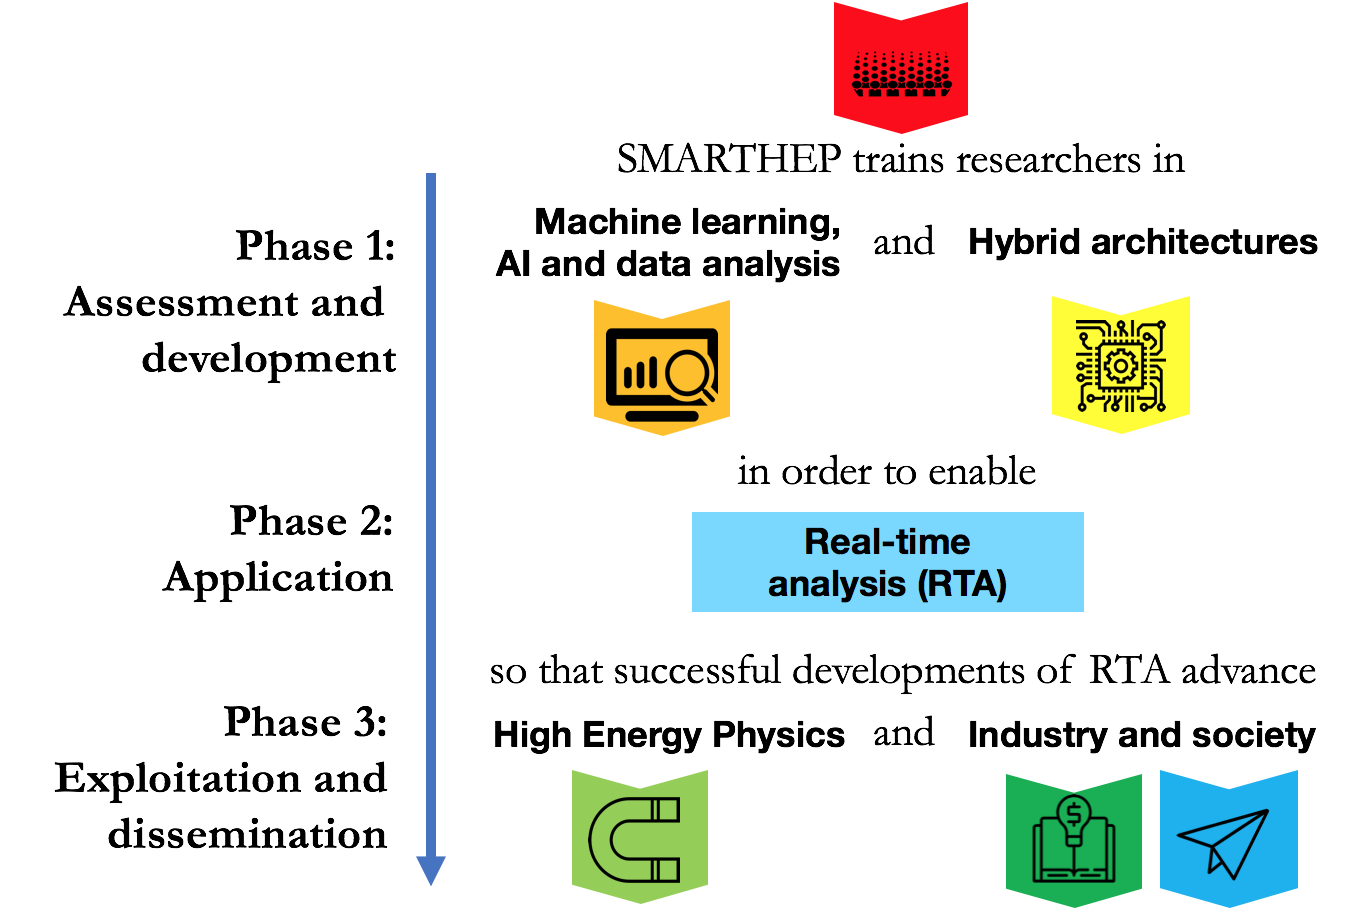
\includegraphics[width=0.49\textwidth]{figs/Implementation.png} %scienceStructure_2.pdf}
%    \vspace{-2mm} 
%	\caption{\acronym implementation strategy.\label{fig:implementation}}
%	\label{fig:scienceStructure.pdf}
%    \vspace{-10mm} 
%\end{wrapfigure}
%
%The connections between the different work packages and the overall \acronym strategy are shown in Fig.~\ref{fig:implementation}.
%Cutting-edge techniques in ML and hybrid architectures will be assessed and developed by the ESRs 
%before their application to specific use cases, in order to enable RTA that advance high energy physics, industry and society, 
%to follow with exploitation and dissemination as described in Sec.~\ref{sec:qualityExploitDissemination}. 
%This modus operandi is at the heart of \acronym and ensures the efficiency of its implementation. 

\subsubsection{Work Packages description}\label{sec:WPdescription}

%Earlier text
\acronym WPs have been introduced in Sec.~\ref{sec:metho}. 
Most ESRs will work on projects which fall within different research WPs, strengthening
\acronym into a coherent whole.
As is clear from our research methodology %and represented in Fig.~\ref{fig:implementation}, 
Real-Time Analysis is the conceptual and technical challenge which permeates all research work packages 
and motivates the network.
\vspace{-5mm}
%\newpage\clearpage
%Table 3.1.a

%WP1
%Description of Work and Role of Specific Beneficiaries / Partner Organisations
%(possibly broken down into tasks), indicating lead participant and role of other participants
\begin{center}\scriptsize
%\resizebox {\textwidth }{!}{%
\begin{tabular}{|p{0.05\textwidth}|p{0.15\textwidth}|p{0.23\textwidth}|p{0.15\textwidth}|p{0.12\textwidth}|}
\hline
\cellcolor{red!70!black} \textbf{\color{white}WP1\color{black}} & \textbf{Management} &  \textbf{Lead Beneficiary}: \lundentity & \textbf{Duration}: 1-48 & 
 ESR: 1 elected
\tabularnewline\hline
\multicolumn{5}{|p{0.975\textwidth}|}{%
\textbf{\Tstrut Objectives:} Create and  maintain a high level of collaboration between the \acronym consortium members to ensure the optimal functioning of the network, and report to the EU on network activities and progress.}\tabularnewline\hline
\multicolumn{5}{|p{0.975\textwidth}|}{\textbf{\Tstrut Description of Work and Role of Partners:}
Doglioni as Project Coordinator (PC) will oversee the smooth running of the planned research and training activities for the network.
\lund has been chosen to coordinate \acronym as a large institution with dedicated support and experience with projects of this kind, and due to Doglioni's experience in coordinating HEP communities and groups within and beyond ATLAS  (e.g. LHC Dark Matter Working Group, more than 300 participants and HEP Software Foundation trigger and reconstruction WG). 
Doglioni is an alumna of the \href{http://www.collegiocavalieri.it/en}{Collegio Universitario Lamaro Pozzani}, funded by the Italian National Federation of Holders of the Order of Merit for Labour and hosting up to 15 selected Italian students per year, complementing their regular university education with courses and lectures in entrepreneurship, law, IT and languages.
This gives her an unique perspective on cross-talk between academia and industry that started developing as early as her undergraduate education. 
Administrative support to the PC will be hired, at the level of at least 50\% FTE. %(\task{1.1}). 
The PC will keep close contact with other WP coordinators to monitor the execution of tasks, and  compliance to the defined milestones.
The PC's first task will be to convene discussions leading to the signature of the Consortium Agreement (CA). %(\task{1.2}).
Management will coordinate the hiring of all ESRs together with a dedicated recruitment officer.% (\task{1.3}, \task{1.4}).
The PC is responsible for preparing and chairing the consortium administrative meetings in the EB and SB, for the preparation of reports for the EU together with the project manager, and for overseeing the election of ESR representatives to the EB and SB. %(\task{1.5}), 
The PC and the relevant WP coordinators oversee the organization of the planned workshops and conferences % (\task{1.6}). 
The PC is responsible for facilitating communication between the nodes, building lasting collaborations between the nodes, enabling knowledge transfer and forming a legacy of future research collaborations.
\Bstrut}\tabularnewline\hline
\multicolumn{5}{|p{0.975\textwidth}|}{
	\pbox{202mm}{\textbf{\Tstrut Deliverables}: \deli{1.1} (month 2) Hiring of a dedicated project manager (month 1); \deli{1.2} Signature of the CA by all parties; }
	}\tabularnewline
\multicolumn{5}{|p{0.975\textwidth}|}{
\deli{1.3} (month 3) Launch of the website and social media accounts as outward-facing communication and organization tools;
}\tabularnewline
\multicolumn{5}{|p{0.975\textwidth}|}{
\deli{1.4} (month 3, 8) Advertisement of the recruitment and recruitment completion, including ESR declarations; 
}\tabularnewline
\multicolumn{5}{|p{0.975\textwidth}|}{
\deli{1.5}  (month 3, 13, 25, 37, 48)  Prepare reports for each SB meeting, incl. mandatory annual and mid-term progress report to EU ; 
}\tabularnewline
\multicolumn{5}{|p{0.975\textwidth}|}{
\deli{1.6}  (month 3, 13, 19, 25, 37, 43, 48)  Collect documentation, reports and feedback following all Network events and schools.
}%%	\pbox{202mm}{}
%%}
\tabularnewline\hline
\end{tabular}
%}%
%\vspace{-8mm}
\end{center}
%Table 3.1.a

%WP2
\begin{center}\scriptsize
\begin{tabular}{|p{0.05\textwidth}|p{0.15\textwidth}|p{0.23\textwidth}|p{0.15\textwidth}|p{0.12\textwidth}|}
\hline

\cellcolor{red} \textbf{\color{white}WP2\color{black}} & \textbf{Training} & \textbf{Lead Beneficiary}: \unige & \textbf{Duration: 1-48} & ESR: All\tabularnewline\hline

\multicolumn{5}{|p{0.975\textwidth}|}{%

\textbf{\Tstrut Objectives:} Organisation of the Network-wide training events, overview of the personal training for each ESR, see Sec.~\ref{sec:training}.}

\tabularnewline\hline
\multicolumn{5}{|p{0.975\textwidth}|}{\textbf{\Tstrut Description of Work and Role of Partners:}
The WP2 coordinator is Sfyrla from \unige, with experience in student supervision, public lectures and course organization. 
The WP2 coordinator oversees the preparation of the Personal Career Development Plans and follows up with the supervisors for the intermediate and final reports %(\task{2.1}). 
Prof. Sfyrla oversees the organization of the lectures for the development of technical, research and transferable skills (see Sec.~\ref{sec:trainingcontrib}) taking place at the Network-wide events. %(\task{2.2})..
The WP2 coordinator makes sure the lecturers give training of excellent quality and that adequate documentation is provided to the ESRs, and provides advertisement and follow-up material together with the PC.  
Short lecture proceedings will be prepared in advance of the lectures by the speakers so that they can be disseminated without delay following the events (as for example with the CHEP conference series). % (\task{2.3}), 
All nodes and partners will benefit and contribute to the training of the ESRs, by playing an active role through supervision of PhD programs, research and industry projects that will train excellent scientists with a wide range of skills and experiences. 
Together with the responsibles for WP7, Sfyrla will ensure the quality and feedback of the presentation of ESRs to \acronym events.% (\task{2.4})
\Bstrut}\tabularnewline\hline
\multicolumn{5}{|p{0.975\textwidth}|}{
	\pbox{202mm}{\textbf{\Tstrut Deliverables}: \deli{2.1}  (month 12, 24, 36, 42)  PCDPs for each ESR, intermediate and final monitoring;}
	}\tabularnewline
\multicolumn{5}{|p{0.975\textwidth}|}{
\deli{2.2}  (month 10, 15, 27-29, 38)  Design and organization of network-wide schools together with responsible beneficiaries;
}\tabularnewline
\multicolumn{5}{|p{0.975\textwidth}|}{
\deli{2.3}  (month 11, 16, 30, 39)  Proceedings of lectures given at the \acronym events; 
}\tabularnewline
\multicolumn{5}{|p{0.975\textwidth}|}{
\deli{2.4}  (month 12, 24, 36, 42)  Presentations from all ESR to the \acronym events and at the final conference;
}
\tabularnewline\hline
\multicolumn{5}{|p{0.975\textwidth}|}{
\deli{2.5} (month 44) ESRs with three-year PhD duration receive a degree.
}
\tabularnewline\hline
\end{tabular}
%\vspace{-9mm}
\end{center}

%%WP3
\begin{center}\scriptsize
\begin{tabular}{|p{0.04\textwidth}|p{0.24\textwidth}|p{0.21\textwidth}|p{0.12\textwidth}|p{0.07\textwidth}|}
\hline

\cellcolor{orange} \textbf{\color{black}WP3\color{black}} & \textbf{ML \& advanced data analysis} & \textbf{Lead Beneficiary}: \cnrs & \textbf{Duration: 8-48} & ESR: All \tabularnewline\hline

\multicolumn{5}{|p{0.975\textwidth}|}{%

\textbf{\Tstrut Objectives:} Deployment of advanced Machine Learning (ML) and data analysis techniques to enable real-time analysis.}

\tabularnewline\hline
\multicolumn{5}{|p{0.975\textwidth}|}{\textbf{\Tstrut Description of Work and Role of Partners:}
The WP3 coordinator is Gligorov from \cnrs, who led the first large-scale implementation of real-time ML at an LHC experiment in 2011, led LHCb's HLT during 2014 and 2015, oversaw LHCb's physics programme as deputy physics coordinator during 2016 and 2017 and is currently leader of the Real Time Analysis Project in LHCb.  
The WP3 coordinator is responsible for the coherence and interaction of the ESRs investigating ML techniques in RTA throughout \acronym, for their development and their application to HEP and commercial use cases according to the network-wide strategy described in Fig.~\ref{fig:implementation}. 
He will also ensure that code is written alongside documentation that makes the software useful and usable, and that frameworks and toolkits are made public in a timely manner and respecting IP clauses in case of commercial exploitation. 
WP3 will produce novel algorithms to reconstruct objects and events in real-time (with the know-how of \nikhefentity and \cernentity), and develop ML techniques for event reconstruction, fast data analysis and outlier detection (exploiting the expertise of \liegesentity, \ibmentity, \fleetmaticsentity and \unigeentity). 
The algorithms for both reconstruction and ML will also be benchmarked and optimized in the projects hosted at \nikhefentity and \cernentity. 
\Bstrut}\tabularnewline\hline
\multicolumn{5}{|p{0.975\textwidth}|}{
\textbf{\Tstrut Deliverables}: \textit{For this and other research WP deliverables, we follow the implementation plan in ~\ref{sec:introRO}, where the ESRs first gain an overview of the state of the art, then developing new techniques, and finally disseminating them as legacy of \acronym.}} 
\tabularnewline
\multicolumn{5}{|p{0.975\textwidth}|}{
\deli{2.2} (joint with WP1, WP2) design, organization and documentation of the contributions to the network ML and MLHEP schools
}\tabularnewline
\multicolumn{5}{|p{0.975\textwidth}|}{
\deli{\deliverableWhitepaperStateOfTheArtWPThree}  (month \deliverableWhitepaperStateOfTheArtWPThreeMonth) 
Whitepaper on the state of the art on ML for real-time analysis, detailing implementation and deployment, capitalizing on the attendance of the MLHEP school in month  24;
}\tabularnewline
\multicolumn{5}{|p{0.975\textwidth}|}{
\deli{\deliverableTriggerExperimentalSoftwareWPThree}  (month \deliverableTriggerExperimentalSoftwareWPThreeMonth) 
Collection of ML algorithms and software toolkits to be exploited for the research objectives in WP5 and WP6; 
}\tabularnewline
\multicolumn{5}{|p{0.975\textwidth}|}{
\deli{\deliverableFinalWhitepaperWPThree}  (month \deliverableFinalWhitepaperWPThreeMonth) .
Review paper collecting description and documentation of techniques for ML in RTA. 
}
\tabularnewline\hline
\end{tabular}
%\vspace{-9mm}
\end{center}


%%WP4
\begin{center}\scriptsize
\begin{tabular}{|p{0.04\textwidth}|p{0.18\textwidth}|p{0.17\textwidth}|p{0.12\textwidth}|p{0.20\textwidth}|}
\hline

\cellcolor{yellow} \textbf{\color{black}WP4\color{black}}  & \textbf{Hybrid architectures} & \textbf{Lead Beneficiary}: \sorbonneentity & \textbf{Duration: 8-48}  & ESR: \ESRsForWPFourText \tabularnewline\hline

\multicolumn{5}{|p{0.975\textwidth}|}{%

\textbf{\Tstrut Objectives:} Study and adoption of hybrid computing architectures to enable RTA.}

\tabularnewline\hline
\multicolumn{5}{|p{0.975\textwidth}|}{\textbf{\Tstrut Description of Work and Role of Partners:}
The WP4 coordinator is Lacassagne from \sorbonneentity. 
He is a system architect with extensive experience in the benchmarking and use of hybrid architectures. 
The WP4 coordinator is responsible for the coherence and interaction of the ESRs developing and testing code for hybrid architectures. 
He is responsible for the  publication and exploitation of successful deliverables related to hybrid architectures, as well as many studies that demonstrated that standard architectures could be improved for the purpose of RTA (see e.g. Lemaitre, Lacassagne, \href{https://hal.archives-ouvertes.fr/hal-01361204/document}{Batched Cholesky Factorization for tiny matrices}, DASIP 2016).
The work is divided in three tasks corresponding to the research objectives: the use of FPGAs (e.g. track triggering for ATLAS, expertise of \ohioentity, \oregonentity, \pisaentity), the use of GPUs for speeding up parallel algorithms in industry and HEP (\santiagoentity), and employing parallel and multithreaded algorithms (\lightboxentity).
Together with the partners, the WP4 coordinator also oversees the training program on each specific architecture, and ensures the quality of lectures and their proceedings with the coordinator of WP2. 
He also makes sure that code written for non-standard architectures satisfies high documentation standards.
\Bstrut}\tabularnewline\hline
\multicolumn{5}{|p{0.975\textwidth}|}{
\textbf{\Tstrut Deliverables}: \deli{2.2} (joint with WP1, WP2) design, organization and documentation of the FPGA and GPU schools.} 
\tabularnewline
\multicolumn{5}{|p{0.975\textwidth}|}{
\deli{\deliverableWhitepaperStateOfTheArtWPFour}  (month \deliverableWhitepaperStateOfTheArtWPFourMonth)  
Whitepaper on the state of the art on hybrid architectures in real-time analysis, capitalizing on attendance of network FPGA/GPU schools;
}\tabularnewline
\multicolumn{5}{|p{0.975\textwidth}|}{
\deli{\deliverableParallelizationOptimizationWPFour}  (month \deliverableParallelizationOptimizationWPFourMonth) 
Software toolkits and hardware improvements in HEP (e.g. FTK for ATLAS, GPU for LHCb reconstruction); 
}\tabularnewline
\multicolumn{5}{|p{0.975\textwidth}|}{
\deli{\deliverableParallelization}  (month \deliverableParallelizationMonth) 
\lightbox software to optimize parallelization of financial transactions and associated publications; 
}\tabularnewline
\multicolumn{5}{|p{0.975\textwidth}|}{
\deli{\deliverableWhitepaperDevelopmentWPFour}  (month \deliverableWhitepaperDevelopmentWPFourMonth)  
Review paper collecting advancements in optimization of hybrid architectures for the LHC trigger systems.
}
\tabularnewline\hline
\end{tabular}
%\vspace{-9mm}
\end{center}

%%WP5
\begin{center}\scriptsize
\begin{tabular}{|p{0.04\textwidth}|p{0.23\textwidth}|p{0.20\textwidth}|p{0.12\textwidth}|p{0.12\textwidth}|}
\hline

\cellcolor{green} \textbf{\color{black}WP5\color{black}} & \textbf{Real-time decision making} & \textbf{Lead Beneficiary}: \dortmundentity & \textbf{Duration: 8-48} 
&   ESR: \ESRsForWPFiveText \tabularnewline\hline

\multicolumn{5}{|p{0.975\textwidth}|}{%

\textbf{\Tstrut Objectives:}  Applying real-time analysis to decision making in physics and society.}

\tabularnewline\hline
\multicolumn{5}{|p{0.975\textwidth}|}{\textbf{\Tstrut Description of Work and Role of Partners:}
WP5's goal is to enable fast and efficient decision making with RTA, in physics through the use of the trigger systems, and in society to improve safety and efficiency of transport in ways that would not be possible without RTA. 
WP5 is coordinated by Albrecht (\dortmundentity as main beneficiary node) with Sopasakis as co-coordinator (\ximantis). 
They have been chosen to fill this role for their complementary expertise in decision-making in HEP and industry that are crucial for \acronym. 
%trigger strategies crucial for the physics analyses in \acronym, and for their expertise on RTA decision-making in transport. 
They will ensure that the RTA techniques enabled by WP3 and WP4 are applied to advance both HEP and industry by the various ESRs working on the experiment trigger systems, that the exchange between academia and industry is fruitful in both directions through cross-pollination of techniques, and that the results are documented in peer-reviewed papers. 
%Together with the WP2 and WP3 coordinators, they oversee the trigger lectures in the introductory event at \lund and the physics and ML school at \unigeshort, and coordinate the preparation of the ISOTDAQ and MLHEP lectures and ESR contributions.
\Bstrut}\tabularnewline\hline
\multicolumn{5}{|p{0.975\textwidth}|}{
\textbf{\Tstrut Deliverables}: \deli{2.2} (joint with WP1, WP2) organization of trigger contributions to network events and ISOTDAQ schools.} 
\tabularnewline
\multicolumn{5}{|p{0.975\textwidth}|}{
\deli{\deliverableWhitepaperStateOfTheArtWPFive}  (month \deliverableWhitepaperStateOfTheArtWPFiveMonth) 
Review of the state of the art of the triggers of LHC collaborations, compiled by ESRs will prior to their physics analyses capitalizing on attendance of ISOTDAQ school and network events; 
}\tabularnewline
\multicolumn{5}{|p{0.975\textwidth}|}{
\deli{\deliverableXimantisHybrid}  (month \deliverableXimantisHybridMonth) 
Improved \ximantisentity app using novel ML techniques (e.g. hybrid networks) and associated publications;
}\tabularnewline
\multicolumn{5}{|p{0.975\textwidth}|}{
\deli{\deliverableTriggerExperimentalSoftwareWPFive}  (month \deliverableTriggerExperimentalSoftwareWPFiveMonth) 
Software for LHC trigger upgrades for Run-3 data taking; 
}\tabularnewline
\multicolumn{5}{|p{0.975\textwidth}|}{
\deli{\deliverableLogisticsOptimisation}  (month \deliverableLogisticsOptimisationMonth) 
Client software for optimization of transport and logistics with \pointeightentity and associated publications;
}
\tabularnewline
\multicolumn{5}{|p{0.975\textwidth}|}{
\deli{\deliverableWhitepaperCollectionPapersWPFive}  (month \deliverableWhitepaperCollectionPapersWPFiveMonth)  
Review paper collecting physics results using trigger selection improvements, including summary of publications on dark sectors, LFV/LFU and precision measurements.}
\tabularnewline\hline

\end{tabular}
%\vspace{-9mm}
\end{center}

%%WP6
\begin{center}\scriptsize
\begin{tabular}{|p{0.04\textwidth}|p{0.3\textwidth}|p{0.18\textwidth}|p{0.12\textwidth}|p{0.2\textwidth}|}
\hline

\cellcolor{cyan} \textbf{\color{black}WP6\color{black}} & \textbf{Real-time monitoring and discoveries} & \textbf{Lead Beneficiary}: \ibm & \textbf{Duration: 8-48} &
ESR: \ESRsForWPSixText \tabularnewline\hline

\multicolumn{5}{|p{0.975\textwidth}|}{%

\textbf{\Tstrut Objectives:}   Applying real-time analysis to monitor complex systems and discover anomalies, in physics and society.}

\tabularnewline\hline
\multicolumn{5}{|p{0.975\textwidth}|}{\textbf{\Tstrut Description of Work and Role of Partners:}
The goal of WP6 is to employ real-time analysis to detect novelty or anomalies while monitoring complex systems and streams of data. 
These data streams range from LHC collision events (\lundentity), to financial transactions (\ibmentity), to data from vehicle dashboard cameras (\fleetmaticsentity), to sensor data from industrial processes (\lightboxentity). 
A sub-goal that is novel to \acronym and essential to introduce such techniques in HEP trigger systems is the accountability and reproducibility of the algorithms employed, developed in \ESRx. 
For this reason, \ibmentity is chosen as the lead beneficiary of WP6 with De Sainte Marie as main coordinator, given his extensive experience in supervision of student projects and his expertise on symbolic knowledge systems. 
WP6's academic co-coordinator is Pierini (\cern), one of the pioneers of anomaly detection in LHC experiments. 
WP6 will work in close collaboration with WP3 to design new algorithms and combine the best of both symbolic knowledge and numerical algorithms towards application to HEP triggers and society. 
The deliverables of WP6 match the research objectives and include applications both in HEP and in the commercial sector, as the algorithms developed can be ported to the different kinds of data. 
Aided by the WP7 coordinator, by LU Innovation from the PC side and by the H2020 IPR helpdesk, WP6 coordinators ensure that these commercial deliverables are disseminated and documented after their exploitation, and correctly handled in terms of IP and \href{http://ec.europa.eu/justice/data-protection/index_en.htm}{EU GDPR}.
\Bstrut}\tabularnewline\hline
\multicolumn{5}{|p{0.975\textwidth}|}{
\textbf{\Tstrut Deliverables}: \deli{2.2} (joint with WP1, WP2) organization of the non-academic training and Industry and career development schools. } 
\tabularnewline
\multicolumn{5}{|p{0.975\textwidth}|}{
\deli{\deliverableWhitepaperStateOfTheArtWPSix} 
Review of the state of the art of fully RTA searches in HEP and recommendations for improvements (companion of \deli{\deliverableWhitepaperStateOfTheArtWPFive})
 (month \deliverableWhitepaperStateOfTheArtWPSixMonth) ; 
}\tabularnewline

\multicolumn{5}{|p{0.975\textwidth}|}{
\deli{\deliverableSoftwareWPSix}  (month \deliverableSoftwareWPSixMonth) 
Software enabling advanced fully RTA-based searches at LHC; 
}\tabularnewline

\multicolumn{5}{|p{0.975\textwidth}|}{
\deli{\deliverableRule}  (month ~\deliverableRuleMonth) 
Algorithms for fraud detection and HEP triggers in \ibmentity and associated publications;
}\tabularnewline

\multicolumn{5}{|p{0.975\textwidth}|}{
\deli{\deliverableFleetmaticsMLMobile}  (month \deliverableFleetmaticsMLMobileMonth) 
Toolkits using ML and AI for real-time in-fleet monitoring within \fleetmaticsentity and associated publications;
}

\tabularnewline
\multicolumn{5}{|p{0.975\textwidth}|}{
\deli{\deliverablePredictiveMaintenance}  (month \deliverablePredictiveMaintenanceMonth) 
Software for sensors for Internet-of-things and industrial process optimization in \lightboxentity 
}
\tabularnewline
\multicolumn{5}{|p{0.975\textwidth}|}{
\deli{\deliverableWhitepaperCollectionPapersWPSix}  (month \deliverableWhitepaperCollectionPapersWPSixMonth)  
Review paper collecting physics results using fully RTA-based analyses, including summary of publications on dark matter mediators, Higgs boson, heavy ion physics. 
%%Companion paper on summary of technical work, and implications outside HEP. 
}
\tabularnewline\hline
\end{tabular}
%\vspace{-9mm}
\end{center}

%%WP7
\begin{center}\scriptsize
\begin{tabular}{|p{0.04\textwidth}|p{0.23\textwidth}|p{0.20\textwidth}|p{0.12\textwidth}|p{0.12\textwidth}|}
\hline

\cellcolor{violet} \textbf{\color{black}WP7\color{black}} & \textbf{Outreach and dissemination} & \textbf{Lead Beneficiary}: \cern & \textbf{Duration: 1-48} & ESR: All ESRs.\tabularnewline\hline

\multicolumn{5}{|p{0.975\textwidth}|}{%


\textbf{\Tstrut Objectives:} Relay \acronym scientific activities to the general public, monitor delivery of results as journal papers, ensure ESR visibility in conferences.}
\tabularnewline\hline

\multicolumn{5}{|p{0.975\textwidth}|}{\textbf{\Tstrut Description of Work and Role of Partners:}
WP7 is detailed further in Sec.~\ref{sec:CommPub}.  
\cern is chosen as the lead beneficiary of WP7 given its extensive experience in communicating with the public, with Petersen as responsible. 
Ustyuzhanin from \yandexentity will co-coordinate the effort benefitting from his extensive expertise with data challenges. 
The WP7 coordinator organise the communication of \acronym to both the general public and the scientific community and ensure that all ESRs and supervisors take part in the effort. 
Together with the PC they run the dedicated communication portal \url{www.smarthep.org}, supported by ESR blogging and social media activities. 
Communication to the scientific communities is achieved by poster and talk contributions to conferences. 
The WP7 coordinator will delegate members of the network to support the ESR supervisors and monitor the quality of the material presented by the ESRs and ensure they benefit from an outstanding international visibility. 
The coordinators will ensure a consistent top quality of papers produced within the Network. 
The main innovation of \acronym's outreach program is the ESR data challenge, organized by \cernentity. 
Further outreach to the general public will take the form of visits to schools, guided visits to CERN facilities, public lectures and "science on tap" at Network events. 
\acronym dissemination activities will be completed by delivery of the specific \acronym Masterclass exercise.
These tasks will ensure the general public grasps the impact of \acronym on academia and HEP, industry and everyday life and actively participates in it through the data challenge.
All academic and industrial partners will take an active part in the WP7 activities, and will simultaneously host online the International Masterclass exercises and World Wide Data Day (WWDD) activities, including on the International Day of Women in Science day.
}\tabularnewline\hline
\multicolumn{5}{|p{0.975\textwidth}|}{
\textbf{\Tstrut Deliverables}: 
\deli{1.3}  (joint with WP1)  Launch of \url{www.smarthep.org} and social media as platform for dissemination, communication and outreach;
}\tabularnewline
\multicolumn{5}{|p{0.975\textwidth}|}{
\deli{7.1}  (month 14)  Data challenge website online and open to the public; 
}\tabularnewline
\multicolumn{5}{|p{0.975\textwidth}|}{
\deli{7.2}  (month 24, 36, 48)  Report on presentation of results at international conferences; 
}\tabularnewline
\multicolumn{5}{|p{0.975\textwidth}|}{
\deli{7.3}  (month 24, 36, 48)  Report on publication of results in peer-reviewed journals; 
}\tabularnewline
\multicolumn{5}{|p{0.975\textwidth}|}{
\deli{7.4}  (month 12, 24, 36, 48)  Reports on outreach to the general public and on \acronym Masterclass/WWDD exercise.
}

\tabularnewline\hline
\multicolumn{5}{p{0.975\textwidth}}{\textbf{Table 3.1a} Work package description for each work package.}
\end{tabular}
%%\vspace{-9mm}
\end{center}

%%Table 3.1.a


%WP0
%Description of Work and Role of Specific Beneficiaries / Partner Organisations
%(possibly broken down into tasks), indicating lead participant and role of other participants
\begin{center}\small
\resizebox {\textwidth }{!}{%
\begin{tabular}{|p{75mm}|p{50mm}|p{25mm}|p{30mm}|}
\hline
\textbf{\Tstrut WP0} & \multicolumn{2}{p{50mm}|}{\textbf{Lead Beneficiary}: \lundentity} & \textbf{Duration: 1-48}\tabularnewline\hline
\textbf{\Tstrut Title: Management} &  Activity type: MGT& \multicolumn{2}{p{45mm}|}{ESR: ---}\tabularnewline\hline
\multicolumn{4}{|p{170mm}|}{%
\pbox{179mm}{\textbf{\Tstrut Objectives:} Create and  maintain a high level of collaboration between the \acronym consortium members to ensure the optimal functioning of the network, as well as report to the EU. }}\tabularnewline\hline
\multicolumn{4}{|p{170mm}|}{
	\pbox{179mm}{\textbf{\Tstrut Description of Work and Role of Partners:}
Dr. C. Doglioni as PC will oversee the smooth running of the planned research and training activities for the network.
\lund has been chosen for the coordination of \acronym and as lead beneficiary of WP0 as it is a large institution with dedicated support and experience
with projects of this kind. 
Administrative support to the PC, at the level of 30\% FTE, will be hired (\task{1.1}). 
She will keep close contact with the coordinators of the other WP to monitor the execution of the tasks, and the compliance to the defined milestones.
The PC will convene the discussions leading to the signature of the Consortium Agreement and the Grant Agreement (\task{1.2}).
Management will coordinate the hiring of all ESRs together with a dedicated recruitment officer (\task{1.3}, \task{1.4}).
The PC will prepare and chair the consortium administrative meetings in the Executive Board and Supervisory Board, 
and will prepare reports to the EU (\task{1.5}). 
%The first of those, the Kick-off meeting is of prime importance to oversee the recruitment of the ESRs.
The PC and the relevant WPCs oversee the organization of planned workshops and conferences  (\task{1.6}). 
Management will ensure optimal communication among the nodes, to 
build lasting collaborations in-between the Network nodes, enabling knowledge transfer and
forming a legacy of future research collaborations.
\Bstrut}}\tabularnewline\hline
\multicolumn{4}{|p{170mm}|}{
	\pbox{179mm}{\textbf{\Tstrut Deliverables:}
\deli{1.1} Hiring of a dedicated project manager (month 1); 
\deli{1.2} Signature of the Consortium Agreement by all parties (month 2); 
\deli{1.3} Launch of the website and Twitter accounts as outward-facing communication and organisation tools (month 3); 
\deli{1.4} Advertisement of the recruitment and recruitment completion (month 3, 6); 
\deli{1.5} Prepare reports for each Supervisory Board meetings, including mandatory annual progress report to EU (months 3, 13, 25, 37, 48); 
\deli{1.6} Collect documentation and reports following all Network events: workshops, conferences, outreach events (months 3, 13, 19, 25, 37,43, 48).\Bstrut}}\tabularnewline\hline
\end{tabular}
}%
\end{center}
%%\clearpage
%%WP5
\begin{center}\small
\resizebox {\textwidth }{!}{%
\begin{tabular}{|p{75mm}|p{50mm}|p{25mm}|p{30mm}|}
\hline
\textbf{\Tstrut WP2} & \multicolumn{2}{p{50mm}|}{\textbf{Lead Beneficiary}: \unige} & \textbf{Duration: 1-48}\tabularnewline\hline
\textbf{\Tstrut Title: Training } &  Activity type: training & \multicolumn{2}{p{45mm}|}{ESR: ALL}\tabularnewline\hline
\multicolumn{4}{|p{170mm}|}{%
\pbox{179mm}{\textbf{\Tstrut Objectives:} Organisation of the Network-wide training events, overview of the personal training for each ESR.
}}\tabularnewline\hline
\multicolumn{4}{|p{160mm}|}{%
\pbox{179mm}{\textbf{\Tstrut Description of Work and Role of Partners:} The main objectives of WP2 are detailed in Sec.~\ref{sec:training}.
As \task{5.1}, the WP2 coordinator is Prof. A. Sfyrla from \unige, with experience in student supervision, public lectures and course organization,
The coordinator oversees the preparation of the Personal Career Development 
Plans and follows up with the supervisors for the intermediate and final reports (\task{2.1}). 
Prof. Sfyrla oversees the organization of the lectures for the development of technical, research and transferable skills
(see Sec.~\ref{sec:trainingcontrib}) taking place at the Network-wide events (\task{2.2}).
The WP2 coordinator makes sure the lecturers give training of excellent quality and that adequate documentation is provided to the ESRs, 
and provides advertisement and follow-up material together with the PC.  
Note that short lecture proceedings will be prepared
in advance of the lectures by the speakers (\task{2.3}), so that they can be disseminated without delay following 
he events (as for example with the CHEP conference series). All nodes and partners will
benefit and contribute to the training of the ESRs, by playing an active role through supervision of
PhD programs, research and industry projects that will train excellent 
scientists with a wide range of skills and experiences. Together with the responsible for WP7, 
Prof. Sfyrla will ensure the quality and feedback of the presentation of ESRs to \acronym events (\task{2.4})
\Bstrut}}\tabularnewline\hline
\multicolumn{4}{|p{160mm}|}{%
\pbox{179mm}{\textbf{\Tstrut Deliverables:} 
%half-time and end
\deli{2.1} Personal Career Development Plans for each ESR, intermediate and final monitoring (month 12, 24, 42)\Bstrut}}\tabularnewline\hline
\deli{2.2} Design and organization of network-wide schools together with beneficiaries responsible \acronym events (months XX, YY);
\deli{2.3} Proceedings of lectures given at the \acronym events (months XX, YY); 
\deli{2.4} Presentations from all ESR to the \acronym events (months 12, 18, 24, 36, 42, 48);
\end{tabular}
}%
\end{center}


%%\clearpage
%%WP3

%Table 3.1.a


%WP0
%Description of Work and Role of Specific Beneficiaries / Partner Organisations
%(possibly broken down into tasks), indicating lead participant and role of other participants
\begin{center}\small
\resizebox {\textwidth }{!}{%
\begin{tabular}{|p{75mm}|p{50mm}|p{25mm}|p{30mm}|}
\hline
\textbf{\Tstrut WP3} & \multicolumn{2}{p{50mm}|}{\textbf{Lead Beneficiary}: \cnrs} & \textbf{Duration: 6-48}\tabularnewline\hline
\textbf{\Tstrut Title: Machine Learning and data analysis } &  Activity type: research & \multicolumn{2}{p{45mm}|}{ESR: ALL}\tabularnewline\hline
\multicolumn{4}{|p{170mm}|}{%
\pbox{179mm}{\textbf{\Tstrut Objectives:} Deployment of advanced Machine Learning techniques to enable Real-Time Analysis.}}\tabularnewline\hline
\multicolumn{4}{|p{170mm}|}{
	\pbox{179mm}{\textbf{\Tstrut Description of Work and Role of Partners:}
The WP3 coordinator is Dr. V. Gligorov from \cnrs, an institute whose members have wide experience in advanced
data analysis and ML techniques. The WP3 coordinator is responsible for the coherence and interaction of the ESRs investigating 
Machine Learning techniques throughout \acronym, for their development and their application to HEP and commercial use cases according to
the network-wide strategy described in Fig.~\ref{fig:implementation}. 
He will also ensure that sustainable code is written alongside documentation that makes the software useful and usable, and  
that frameworks and toolkits are made public in a timely manner and respecting IP clauses in case of commercial exploitation. 
\Bstrut}}\tabularnewline\hline
\end{tabular}
}%
\end{center}
\newpage
\begin{center}\small
\resizebox {\textwidth }{!}{%
\begin{tabular}{|p{75mm}|p{50mm}|p{25mm}|p{30mm}|}
\hline
\multicolumn{4}{|p{160mm}|}{%
%\pbox{179mm}
{\textbf{\Tstrut Deliverables:} 
Deliverables of WP3 include ML software for the improvement of jet reconstruction and tagging in CMS and
related technical publications (\deli{\deliverableCMSHLTDNNJEC}, \deli{\deliverableHEPPubCMSHLTDNNJEC}, \deli{\deliverableCMSHLTGeneralPurposeScouting}), 
the creation of toolkits for trigger optimization (\deli{\deliverableTechPubMLForOptimisation}, \deli{\deliverableTriggerOptToolkit})
and publications related to the commercial software for the creation of 
adversarial networks examples and combination of
time-ordered and non-time-ordered sources in industry and HEP in collaboration with WP6 (\deli{\deliverableTechPubAdversarialFramework}, \deli{\deliverableTechPubTimeOrderedSourcesFramework})
%and relative peer-reviewed publications on physics applications in collaboration with WP5. 
}}\tabularnewline\hline
\end{tabular}
}%
\end{center}
%%\clearpage
%%Table 3.1.a
%WP4
%Description of Work and Role of Specific Beneficiaries / Partner Organisations
%(possibly broken down into tasks), indicating lead participant and role of other participants
\begin{center}\small
\resizebox {\textwidth }{!}{%
\begin{tabular}{|p{75mm}|p{50mm}|p{25mm}|p{30mm}|}
\hline
\textbf{\Tstrut WP4} & \multicolumn{2}{p{50mm}|}{\textbf{Lead Beneficiary}: \cnrs} & \textbf{Duration: 6-48}\tabularnewline\hline
\textbf{\Tstrut Title: Hybrid Architectures} &  Activity type: research & \multicolumn{2}{p{45mm}|}{ESR: ALL}\tabularnewline\hline
\multicolumn{4}{|p{170mm}|}{%
\pbox{179mm}{\textbf{\Tstrut Objectives:} Study of hybrid computing architectures to enable Real-Time Analysis.}}\tabularnewline\hline
\multicolumn{4}{|p{170mm}|}{
	\pbox{179mm}{\textbf{\Tstrut Description of Work and Role of Partners:}
	%Split into tasks
The WP4 coordinator is Dr. L. Lacassagne from \cnrs. He is a system architect with extensive experience in
the benchmarking and use of hybrid architectures. 
The WP4 coordinator is responsible for the coherence and interaction of the ESRs developing code and testing it on systems that are 
not only composed of ordinary CPUs, following the strategy described in Fig.~\ref{fig:implementation}. 
He is responsible for the  publication and exploitation of successful deliverables related to hybrid architectures, 
as well as many studies that demonstrated that standard architectures are not as well suited for the purpose of real-time analysis. 
Together with the \ohio, \santiago and \pisa partners oversees the training programme on 
each specific architecture (FPGA), and ensures the quality of lectures and their proceedings with the coordinator of WP2. 
He also makes sure that code written for non-standard architectures satisfies sustainability and documentation standards.  
\Bstrut}}\tabularnewline\hline
\end{tabular}
}%
\end{center}
\newpage
\begin{center}\small
\resizebox {\textwidth }{!}{%
\begin{tabular}{|p{75mm}|p{50mm}|p{25mm}|p{30mm}|}
\hline
\multicolumn{4}{|p{160mm}|}{%
%\pbox{179mm}
{\textbf{\Tstrut Deliverables:} 
Deliverables of WP4 include the creation of toolkits for the optimization of specific hybrid architectures in HEP like the ATLAS FTK (\deli{\deliverableToolkitTrainingFTK}),
and for more general benchmarking (\deli{\deliverableTechPubHybrid}). Publications concerning multithreading (\deli{\deliverableTechPubMultithreaded}) and 
applications of hybrid architectures in the ATLAS and LHCb triggers are also under the purview of WP4 (\deli{\deliverableTechPubLLPGPU)}, \deli{\deliverableHEPPubATLASFTK}, \deli{\deliverableHEPPubHybrid}). 
The related HEP publications are deliverables in collaboration with WP5. A joint deliverable of WP2 and WP4 is the design, organization and documentation of the FPGA and GPU schools (\deli{2.2}). 
}}\tabularnewline\hline
\end{tabular}
}%
\end{center}

%%\clearpage
%%WP3

%Table 3.1.a


%WP0
%Description of Work and Role of Specific Beneficiaries / Partner Organisations
%(possibly broken down into tasks), indicating lead participant and role of other participants
\begin{center}\small
\resizebox {\textwidth }{!}{%
\begin{tabular}{|p{75mm}|p{50mm}|p{25mm}|p{30mm}|}
\hline
\textbf{\Tstrut WP5} & \multicolumn{2}{p{50mm}|}{\textbf{Lead Beneficiary}: \helsinki} & \textbf{Duration: 6-48}\tabularnewline\hline
\textbf{\Tstrut Title: Physics Applications} &  Activity type: research & \multicolumn{2}{p{45mm}|}{ESR: ALL}\tabularnewline\hline
\multicolumn{4}{|p{170mm}|}{%
\pbox{179mm}{\textbf{\Tstrut Objectives:} Physics applications of Real-Time Analysis.}}\tabularnewline\hline
\multicolumn{4}{|p{170mm}|}{
	\pbox{179mm}{\textbf{\Tstrut Description of Work and Role of Partners:}
	%Split into tasks
WP5's first task is to form a coherent inter-experiment strategy for tackling crucial questions in HEP that uses complementary information from all LHC experiments. The WP5 coordinators are one per LHC experiment, namely Dr. M. Dunford (ATLAS), M. Voutilainen (CMS) (main coordinator), J. Albrecht (LHCb), P. Christiansen (ALICE). They have been chosen to fill this role for their expertise in real-time analysis and in the physics analyses that are focus of \acronym. Their task is to ensure that LHC data is fully exploited in HEP searches and measurements thanks to RTA techniques enabled by WP3 and WP4, and the results documented in peer-reviewed papers. Together with WP2, they oversee the physics lectures in the introductory school at \lund and the physics and ML school at \unigeshort. 
\Bstrut}}\tabularnewline\hline
\end{tabular}
}%
\end{center}
\newpage
\begin{center}\small
\resizebox {\textwidth }{!}{%
\begin{tabular}{|p{75mm}|p{50mm}|p{25mm}|p{30mm}|}
\hline
\multicolumn{4}{|p{160mm}|}{%
%\pbox{179mm}
{\textbf{\Tstrut Deliverables:} 
Deliverables of WP4 include publications on detector and reconstruction developments with RTA,
(\deli{\deliverableHEPPubALICETPC}, \deli{\deliverableHEPPubLFVReco}),
dark sectors and Higgs boson searches
(\deli{\deliverableHEPPubATLASTLAFTK}, \deli{\deliverableHEPPubATLASTLAMultijet}, \deli{\deliverableHEPPubLLP}),
Lepton Flavor Violation  
(\deli{\deliverableHEPPubLFVFlavored}, \deli{\deliverableHEPPubLFVUnflavored}, \deli{\deliverableHEPPubLFV}, \deli{\deliverableHEPPubLFVATLAS}),
and precision measurements
(\deli{\deliverableHEPPubALICEPhysics}) 
A joint deliverable of WP2 and WP5 is the design, organization and documentation of the physics lectures in the introductory and Physics/ML schools (\deli{2.2}). 
}}\tabularnewline\hline
\end{tabular}
}%
\end{center}


%%WP0
%%Description of Work and Role of Specific Beneficiaries / Partner Organisations
%%(possibly broken down into tasks), indicating lead participant and role of other participants
%\begin{center}\small
%\resizebox {\textwidth }{!}{%
%\begin{tabular}{|p{75mm}|p{50mm}|p{25mm}|p{30mm}|}
%\hline
%\textbf{\Tstrut WP5} & \multicolumn{2}{p{50mm}|}{\textbf{Lead Beneficiary}: \helsinki} & \textbf{Duration: 6-48}\tabularnewline\hline
%\textbf{\Tstrut Title: Physics Applications} &  Activity type: research & \multicolumn{2}{p{45mm}|}{ESR: ALL}\tabularnewline\hline
%\multicolumn{4}{|p{170mm}|}{%
%\pbox{179mm}{\textbf{\Tstrut Objectives:} {Physics applications of Real-Time Analysis.}}\tabularnewline\hline
%\multicolumn{4}{|p{170mm}|}{
%	\pbox{179mm}{\textbf{\Tstrut Description of Work and Role of Partners:}
%	%Split into tasks
%\Bstrut}}\tabularnewline\hline
%\end{tabular}
%}%
%\end{center}
%\newpage
%\begin{center}\small
%\resizebox {\textwidth }{!}{%
%\begin{tabular}{|p{75mm}|p{50mm}|p{25mm}|p{30mm}|}
%\hline
%\multicolumn{4}{|p{160mm}|}{%
%%\pbox{179mm}
%{\textbf{\Tstrut Deliverables:} 
%MISSING HELSINKI AND LUND 
%Deliverables of WP4 include publications on detector and reconstruction developments with RTA,
%(\deli{\deliverableHEPPubALICETPC}, \deli{\deliverableHEPPubLFVReco}),
%dark sectors and Higgs boson searches
%(\deli{\deliverableHEPPubATLASTLAFTK}, \deli{\deliverableHEPPubATLASTLAMultijet}, \deli{\deliverableHEPPubLLP}),
%Lepton Flavor Violation  
%(\deli{\deliverableHEPPubLFVFlavored}, \deli{\deliverableHEPPubLFVUnflavored}, \deli{\deliverableHEPPubLFV}, \deli{\deliverableHEPPubLFVATLAS}),
%and precision measurements
%(\deli{\deliverableHEPPubALICEPhysics}) 
%A joint deliverable of WP2 and WP5 is the design, organization and documentation of the physics lectures in the introductory and Physics/ML schools (\deli{2.2}). 
%}}\tabularnewline\hline
%\end{tabular}
%}%
%\end{center}
%%\clearpage
%%WP6
\begin{center}\small
\resizebox {\textwidth }{!}{%
\begin{tabular}{|p{75mm}|p{50mm}|p{25mm}|p{30mm}|}
\hline
\textbf{\Tstrut WP6} & \multicolumn{2}{p{50mm}|}{\textbf{Lead Beneficiary}: \dq} & \textbf{Duration: 6-48}\tabularnewline\hline
\textbf{\Tstrut Title: Industrial applications of RTA} &  Activity type: OUT & \multicolumn{2}{p{45mm}|}{ESR: ALL}\tabularnewline\hline
\multicolumn{4}{|p{170mm}|}{%
\pbox{179mm}{\textbf{\Tstrut Objectives:} Exploit advancements of RTA from HEP to industrial applications and vice versa.\Bstrut}}\tabularnewline\hline
\multicolumn{4}{|p{160mm}|}{%
%	\multicolumn{8}{l}{\pbox{21cm}{\small R: Report, ADM: Administrative; PDE: dissemin.; PU: Public; CO: Confidential, restricted to consortium and Commission services}}\tabularnewline
\pbox{179mm}{\textbf{\Tstrut Description of Work and Role of Partners:} 
\dq is chosen as the lead beneficiary of WP6 with N. Meric as contact,
following the Prix AirFrance awards at the 2015 Web Summit, 
given their experience in technology transfer, 
and the extensive past and present experience of their members in both industry and HEP. 
They receive the support of a second coordinator, P. Starovoitov from \heidelberg
with complementary expertise, ensuring that the exchange between academia and industry is fruitful 
in both directions. The WP6 coordinators follow the industrial secondments and 
have a coherent view of the deliverables so that they fit within the overall network programme. 
The deliverables of WP6 match the research objectives and include all commercial applications of RTA: 
they consist of toolkits within ML and AI for mobile platform, 
RTA for medical and financial application and for process optimization (\task{6.1}-\task{6.4}). 
The WP6 coordinators ensure that these commercial deliverables are disseminated and documented after 
their exploitation, as well as correctly handled in terms of IP. The WP6 coordinators maintain the communications with the European IPR Helpdesk. 
They organize the \acronym school focused on industrial and commercials topics (\task{6.5}). 
}}\tabularnewline\hline
\end{tabular}
}%
\end{center}
\newpage
\begin{center}\small
\resizebox {\textwidth }{!}{%
\begin{tabular}{|p{75mm}|p{50mm}|p{25mm}|p{30mm}|}
\hline
\multicolumn{4}{|p{160mm}|}{%
%\pbox{179mm}
{\textbf{\Tstrut Deliverables:} 
To be completed...
Commercial 
software for the creation of adversarial networks examples and combination of
time-ordered and non-time-ordered sources in industry and HEP (\deli{\deliverableAdversarialFramework}, \deli{\deliverableTimeOrderedSourcesFramework})
\Bstrut}}\tabularnewline\hline
\end{tabular}
}%
\end{center}



%%\clearpage
%%WP6
\begin{center}\small
\resizebox {\textwidth }{!}{%
\begin{tabular}{|p{75mm}|p{50mm}|p{25mm}|p{30mm}|}
\hline
\textbf{\Tstrut WP7} & \multicolumn{2}{p{50mm}|}{\textbf{Lead Beneficiary}: \cern} & \textbf{Duration: 1-48}\tabularnewline\hline
\textbf{\Tstrut Title: Outreach and dissemination} &  Activity type: OUT & \multicolumn{2}{p{45mm}|}{ESR: ALL}\tabularnewline\hline
\multicolumn{4}{|p{170mm}|}{%
\pbox{179mm}{\textbf{\Tstrut Objectives:} Relay the scientific activities of \acronym to the general public, monitor the delivery of the results as journal papers, ensure the visibility of the ESR in conferences.\Bstrut}}\tabularnewline\hline
\multicolumn{4}{|p{160mm}|}{%
%	6.1 & Website completion and creation of Facebook and Twitter accounts & ADM & PU & 3 & 6 & \dq & The web page becomes public and is reinforced by accounts in the Social Networks \tabularnewline\midrule
%	6.2 & Talks and posters in conferences & PDE & PU & 12-48 & 6 & \dq & The ESRs will present \acronym\ research in Excellence conferences \tabularnewline\midrule
%	6.3 & Publications in journals & PDE & PU & 12-48 & 6 & \dq & The results of our research will produce scientific papers to be published in reference journals \tabularnewline\midrule
%	6.4 & Outreach: open talks during Network-wide events and visits to schools & PDE & PU & 6-48 & 6 & \dq & \acronym\ will prioritise making the general public aware of our activities \tabularnewline\midrule
%	6.5 & Outreach: \acronym Masterclass exercise & PDE & PU & 42 & 6 & \cern & design and implement a Masterclass exercise highlighting \acronym methods \tabularnewline\midrule
%	\multicolumn{8}{l}{\pbox{21cm}{\small R: Report, ADM: Administrative; PDE: dissemin.; PU: Public; CO: Confidential, restricted to consortium and Commission services}}\tabularnewline
\pbox{179mm}{\textbf{\Tstrut Description of Work and Role of
    Partners:}  
WP7 is detailed further in Sec.~\ref{sec:CommPub}. 
\cern is chosen as the lead beneficiary of WP7
%following the Prix AirFrance awards at the 2015 Web Summit and 
given their extensive experience in communicating with the public. 
The WP6 coordinator organises the communication of \acronym to two main audiences: the general public and the scientific community.  
%The \url{www.smarthep.org} is instrumental in both cases, hence 
\task{6.1} consists in setting up a dedicated outreach portal together with the PC for 
the communication platform \url{www.smarthep.org}, which is supported by social media activities.
The communication to the scientific communities is achieved by poster and talk contributions to conferences. The coordinator will monitor the quality of the material presented by the ESRs and make sure they benefit from a outstanding international visibility (\task{6.2}). 
A crucial scientific deliverable will be the articles reporting on the activities of the Network. As \task{6.3}, the coordinator will ensure a consistent top quality of the paper produced within the Network. The outreach to the general public will take the form of visits to schools, guided visits to the CERN facilities, and the public lectures and "science on tap" at the network events (\task{6.4}). The dissemination activities of \acronym will completed by the delivery of the \acronym Masterclass exercise (\task{6.5}). These tasks will ensure that the general public will grasp the impact of \acronym on academia and HEP, industry and everyday life. All academic and industrial partners will take an active part in the WP7 activities, and in particular they will simultaneously host 
%provide the material and local connection for 
the International Masterclass exercise. 
}}\tabularnewline\hline
\end{tabular}
}%
\end{center}
\newpage
\begin{center}\small
\resizebox {\textwidth }{!}{%
\begin{tabular}{|p{75mm}|p{50mm}|p{25mm}|p{30mm}|}
\hline
\multicolumn{4}{|p{160mm}|}{%
%\pbox{179mm}
{\textbf{\Tstrut Deliverables:} 
\deli{6.1} \url{www.smarthep.org} and Facebook and Twitter accounts as a platform for outreach (month 3);
\deli{6.2} Talks and Posters in conferences (month 12-48); 
\deli{6.3} Publication of scientific results in peer-reviewed journals (month 12-48); 
\deli{6.4} Outreach to the general public (month 6-48).
\deli{6.5} Deliver \acronym Masterclass exercise (month 42).
\Bstrut}}\tabularnewline\hline
\end{tabular}
}%
\end{center}




\FloatBarrier
%\clearpage

\subsubsection{List of major deliverables}

%A deliverable is a distinct output of the action, meaningful in terms of the action?s overall objectives and constituted by a report, a document, a technical diagram, a software, training, conference, etc. These should be divided into scientific deliverables and management, training, recruitment and dissemination deliverables. Scientific deliverables have technical/scientific content specific to the action. The number of deliverables in a given Work Package must be reasonable and commensurate with the Work Package content. Note that during implementation, the submission of these deliverables to the REA will be a contractual obligation.
%Table 3.1.b, Including the awarding of doctoral degrees!
\vspace{-1mm}
The following tables lists the major deliverables of the project. 

\color{blue}\noindent Scientific Deliverables\color{black}\addtocounter{table}{1}\vspace{-11mm}\\
\begin{center}
\resizebox {\textwidth }{!}{%
\begin{tabular}{@{}p{5mm}@{~~}p{60mm}p{6mm}p{18mm}p{6mm}cp{8mm}p{90mm}@{}}
\toprule
\multicolumn{2}{l}{\pbox{8cm}{Deliverable\\Number \& Title}} &
%Deliverable numbers in order of delivery dates. Please use the numbering convention <WP number>.<number of deliverable within that WP>. For example, deliverable 4.2 would be the second deliverable from Work Package 4.
WP &
\pbox{8cm}{\Tstrut Lead Benef.\\Short Name\Bstrut}& %\\Short\\Name
\multicolumn{2}{c}{\pbox{8cm}{Type \& Dissemin.\\Level}}&
%Type: Please indicate the nature of the deliverable using one of the following codes:
%R = Report; ADM = Administrative (website completion, recruitment completion, etc.); PDE = dissemination and/or exploitation of results; OTHER = Other, including coordination 

%Dissemination level:
%Please indicate the dissemination level using one of the following codes:	
%PU = Public: fully open, e.g. web; CO = Confidential: restricted to consortium, other designated entities (as appropriate) and Commission %services; Please consider that deliverables marked as "PU" will automatically be published on CORDIS once approved: the applicants should %therefore consider the relevance of marking a deliverable as "PU";
%CI = Classified: classified information as intended in Commission Decision 2001/844/EC. 
\pbox{8cm}{Due\\Date} & 
Description\tabularnewline 
\toprule

%WP3

\deliverableWhitepaperStateOfTheArtWPThree & Whitepaper on the state of the art of Machine Learning (ML) and data analysis & 3 & \cnrs & R & PU & \deliverableWhitepaperStateOfTheArtWPThreeMonth & Publication of whitepaper summarizing the state of the art in ML techniques for RTA \tabularnewline\midrule 
\deliverableTriggerExperimentalSoftwareWPThree & Software for experiment real-time systems & 3 & \cnrs & OTHER & CO & \deliverableTriggerExperimentalSoftwareWPThreeMonth & Deployment of software enabling RTA at LHC before data taking \tabularnewline\midrule 
\deliverableWhitepaperDevelopmentWPThree & Whitepaper with results from ML application to real-time systems & 3 & \cnrs & PDE & PU & \deliverableWhitepaperDevelopmentWPThreeMonth & Publication of whitepaper collecting ML and reconstruction advancements from ESR projects \tabularnewline\midrule 

%\deliverableCMSHLTDNNJEC  & Software for DNN in CMS object reconstruction & 3 & \cnrs, \helsinki & R & PU & 24 & Release of CMS software for improvement of jet calibration \tabularnewline\midrule 
%\deliverableCMSHLTGeneralPurposeScouting  & Software for CMS trigger & 3 & \cnrs, \helsinki & R & PU & 32 & Release of CMS software for general purpose scouting dataset, supplemented with heavy object/flavor tagging information \tabularnewline\midrule 
%\deliverableLLPTrackingToolkit & Software for tracking in ATLAS trigger & 3 & \cnrs, \unige & R & PU & 24 & Release of ATLAS software for tracking in trigger, including long-lived particles\tabularnewline\midrule
%\deliverableTriggerOptToolkit & Toolkit for trigger optimization & 3 & \cnrs, \nikhef & R & PU & 30 & Release of toolkit for automatic coptimization of trigger systems\tabularnewline\midrule
%\deliverableTechPubMLForOptimisation & Publication related to \deliverableTriggerOptToolkit & 3 & \cnrs, \nikhef & R & PU & 34 & Publication documenting the automatic optimization of trigger systems\tabularnewline\midrule
%\deliverableTechPubAdversarialFramework & Publication related to \deliverableAdversarialFramework & 3 & \cnrs & R & PU & 32 & Publication documenting intersector toolkit for creation of adversarial network examples\tabularnewline\midrule
%\deliverableTechPubTimeOrderedSourcesFramework & Publication related to \deliverableTimeOrderedSourcesFramework & 3 & \cnrs & R & PU & 32 & Release of intersector toolkit for combination of time-ordered and non-time-ordered sources in industry and HEP\tabularnewline\midrule

%WP4

\deliverableWhitepaperStateOfTheArtWPFour & Whitepaper on the state of the art of Machine Learning (ML) and data analysis & 3 & \sorbonneentity & R & PU & \deliverableWhitepaperStateOfTheArtWPFourMonth & Publication of whitepaper summarizing the state of the art in ML techniques for RTA \tabularnewline\midrule 
\deliverableWhitepaperDevelopmentWPFour & Whitepaper with results from application of hybrid architectures to real-time systems & 3 & \sorbonneentity & PDE & PU & \deliverableWhitepaperDevelopmentWPFourMonth & Publication of whitepaper collecting advancements in hybrid architectures from ESR projects \tabularnewline\midrule 
\deliverableParallelizationOptimizationWPFour & Toolkit for hybrid architectures & 3 & \sorbonneentity & OTHER & PU & \deliverableParallelizationOptimizationWPFourMonth & Release of intersector toolkit for benchmarking and optimization of hybrid architectures \tabularnewline\midrule 

%\deliverableTechPubLLPGPU & Publication on ATLAS trigger tracking & 4 & \cnrs, \unige & R & PU & 30 & Documentation of testing of ATLAS tracking algorithms on GPU \tabularnewline\midrule
%\deliverableTechPubMultithreaded & Software for multithreading in ATLAS trigger system & 4 & \cnrs, \cern & R & PU & 30 & Release of toolkit for optimization of creation of FTK pattern banks\tabularnewline\midrule
%\deliverableToolkitTrainingFTK & Software for optimization of FTK & 4 & \cnrs & R & PU & 28 & Release of software for optimization of creation of FTK pattern banks in ATLAS\tabularnewline\midrule
%\deliverableHEPPubATLASFTK & Documentation of \deliverableToolkitTrainingFTK & 4 & \cnrs & R & PU & 34 & Publication on generation of FTK pattern banks using industrial-grade parallelization frameworks\tabularnewline\midrule
%\deliverableToolkitHybrid & Toolkit for hybrid architectures & 4 & \cnrs & R & PU & 28 & Intersector toolkit for benchmarking and optimization of hybrid architectures\tabularnewline\midrule
%\deliverableTechPubHybrid & Publication related to \deliverableTimeOrderedSourcesFramework & 4 & \cnrs & R & PU & 28 & Publication documenting intersector toolkit for benchmarking and optimization of hybrid architectures\tabularnewline\midrule
%\deliverableHEPPubHybrid & Publication related to \deliverableTimeOrderedSourcesFramework in HEP & 4 & \cnrs & R & PU & 40 & Publication documenting technical HEP use cases of toolkit for benchmarking and optimization of hybrid architectures\tabularnewline\midrule

%WP5

\deliverableWhitepaperStateOfTheArtWPFive & Whitepaper on the state of the art physics analysis with real-time objects & 3 & \helsinki & R & PU & \deliverableWhitepaperStateOfTheArtWPFiveMonth & Publication of whitepaper summarizing the state of the art in LHC searches and measurements using RTA \tabularnewline\midrule 
\deliverableWhitepaperCollectionPapersWPFive &  Whitepaper with \acronym results of RTA to physics problems & 3 & \helsinki & PDE & PU & \deliverableWhitepaperCollectionPapersWPFiveMonth & Publication of whitepaper collecting summaries of peer-reviewed results from physics analysis within \acronym  \tabularnewline\midrule 

%WP6
\deliverableLogisticsOptimisation & Study of use of RTA in logistics and transport  & 6 & \pointeightentity & OTHER & PU & \deliverableLogisticsOptimisationMonth & Software and publication of optimisation of logistics and transport using ML and RTA. \tabularnewline\midrule
\deliverablePredictiveMaintenance & \lightbox IoT-based industrial maintenance software & 6 & \dqentity & OTHER & CO & \deliverablePredictiveMaintenanceMonth & Release of \lightboxentity software for predictive maintenance of industrial processes \tabularnewline\midrule
\deliverableFleetmaticsMLMobile  & \fleetmatics Contribution to ML in-vehicle image processing and website & 6 & \dqentity & OTHER & CO & \deliverableFleetmaticsMLMobileMonth & Contribution to \fleetmaticsentity app using ML toolkits for in-vehicle image processing and online learning website\tabularnewline\midrule
\deliverableParallelization & \lightboxentity software for real-time task parallelization & 6 & \dqentity & OTHER & CO & \deliverableParallelizationMonth & Release of \lightboxentity toolkit to improve the efficiency of a simulated task in real-time \tabularnewline\midrule
\deliverableXimantisML & \ximantis app with re-trained AI & 6 & \dqentity & OTHER & CO & \deliverableXimantisMLMonth & Contribution to \ximantisentity app using Convolutional NNs \tabularnewline\midrule
\deliverableXimantisHybrid & \ximantis app using hybrid network & 6 & \dqentity & OTHER & CO & \deliverableXimantisHybridMonth & Contribution to \ximantisentity app using Hybrid networks\tabularnewline\midrule
\deliverableDashboardCam & \fleetmatics software & 6 & \dqentity & OTHER & CO & \deliverableDashboardCamMonth & Contribution to software for dashboard cameras for in-fleet monitoring \tabularnewline\midrule
\deliverableRule & Implementation of algorithms that combine of symbolic knowledge and analytics models & 6, 3 & \ibmentity & OTHER & PU & \deliverableNNMonth & Release implementation of algorithms (commercial and demo) combining symbolic knowledge and analytics models\tabularnewline\midrule

%\deliverableTimeOrderedSourcesFramework & Toolkit for combination of sources in ML & 6, 3 & \dqentity & R & PU & XX & Release of \dq intersector toolkit for combination\tabularnewline\midrule

%\deliverableHEPPubALICETPC & Publication on ALICE TPC & 5 & \helsinkientity, \lundentity & R & PU & 24 & Publication on real-time calibration of ALICE TPC \tabularnewline\midrule
%\deliverableHEPPubLFVReco & Publication on LHCb reconstruction in trigger & 5 & \helsinkientity, \cern & R & PU & 24 & Documentation of LHCb trigger tracking algorithms for low energy particles \tabularnewline\midrule
%\deliverableHEPPubCMSHLTDNNJEC  & Publication on DNN in CMS object reconstruction & 3, 5 & \cnrs, \helsinki & R & PU & 26 & Publication related to CMS software for improvement of jet calibration \tabularnewline\midrule 
%
%\deliverableHEPPubLLP & Publication on Dark Sector long-lived particle search & 5 & \helsinkientity, \unige & R & PU & 40 & Publication of ATLAS Dark Sector search with RTA long-lived particle algorithms in trigger\tabularnewline\midrule
%\deliverableHEPPubATLASTLAFTK & Publication on dijet Dark Matter search & 5 & \helsinkientity, \cnrs & R & PU & 40 & Publication of ATLAS Dark Matter search exploiting FTK in dijet final states \tabularnewline\midrule
%\deliverableHEPPubATLASTLAMultijet & Publication on multijet Dark Matter search & 5 & \helsinkientity, \heidelberg & R & PU & 30 & Publication of ATLAS Dark Matter search in multijet final states at the trigger level \tabularnewline\midrule
\label{tab:DeliverList}
\end{tabular}
}%
\vspace{-8mm}
\end{center}
%
%\noindent Scientific Deliverables (contd) \addtocounter{table}{1}\vspace{-6mm}\\
%\begin{center}
%\resizebox {\textwidth }{!}{%
%\begin{tabular}{@{}p{5mm}@{~~}p{60mm}p{6mm}p{12mm}p{16mm}cp{15mm}p{80mm}@{}}
%\toprule
%\multicolumn{2}{l}{\pbox{8cm}{Deliverable\\Number \& Title}} &
%%Deliverable numbers in order of delivery dates. Please use the numbering convention <WP number>.<number of deliverable within that WP>. For example, deliverable 4.2 would be the second deliverable from Work Package 4.
%WP &
%\pbox{8cm}{\Tstrut Lead\\Benef.\\Short\\Name\Bstrut}&
%\multicolumn{2}{c}{\pbox{8cm}{Type \&\\Dissemin.\\Level}}&
%%Type: Please indicate the nature of the deliverable using one of the following codes:
%%R = Report; ADM = Administrative (website completion, recruitment completion, etc.); PDE = dissemination and/or exploitation of results; OTHER = Other, including coordination 
%%Dissemination level:
%%Please indicate the dissemination level using one of the following codes:	
%%PU = Public: fully open, e.g. web; CO = Confidential: restricted to consortium, other designated entities (as appropriate) and Commission %services; Please consider that deliverables marked as "PU" will automatically be published on CORDIS once approved: the applicants should %therefore consider the relevance of marking a deliverable as "PU";
%%CI = Classified: classified information as intended in Commission Decision 2001/844/EC. 
%\pbox{8cm}{Due\\Date} & 
%Description\tabularnewline 
%\toprule
%
%\deliverableHEPPubCMSDijet & Publication on dijet Dark Matter search & 5 & \helsinkientity & R & PU & 30 & Publication of CMS Dark Matter search in dijet final states at the trigger level \tabularnewline\midrule
%\deliverableHEPPubCMSBoosted & Publication on Higgs boson and Z measurements & 5 & \helsinkientity & R & PU & 30 & Publication of CMS Higgs and Z boson trigger-level measurements, decaying in heavy flavor quarks \tabularnewline\midrule
%
%\deliverableHEPPubLFVFlavored & Publication on Lepton Flavor Violation in flavored mesons  & 5 & \helsinkientity, \cern & R & PU & 40 & Publication on Lepton Flavor Violation using flavored meson decays in LHCb \tabularnewline\midrule
%\deliverableHEPPubLFVUnflavored & Publication on Lepton Flavor Violation in unflavored mesons & 5 & \helsinkientity, \dortmund & R & PU & 40 & Publication on Lepton Flavor Violation using unflavored meson decays in LHCb \tabularnewline\midrule
%\deliverableHEPPubLFV & Publication on Lepton Flavor Violation in tau to muon+photon & 5 & \helsinkientity, \nikhef & R & PU & 40 & Publication on Lepton Flavor Violation in tau to muon+photon in LHCb \tabularnewline\midrule
%\deliverableHEPPubLFV & Publication on Lepton Flavor Violation in tau to three muons & 5 & \helsinkientity, \nikhef & R & PU & 40 & Publication on Lepton Flavor Violation in ATLAS \tabularnewline\midrule
%
%\deliverableHEPPubALICEPhysics & ALICE Publication on nuclear modification factor & 5 & \helsinkientity, \lundentity & R & PU & 40 & ALICE Publication on nuclear modification factor with RTA in Run-3 data \tabularnewline\midrule
%
%%WP6
%
%\multicolumn{8}{l}{\pbox{21cm}{\small R: Report, ADM: Administrative; PDE: dissemin.; PU: Public; CO: Confidential, restricted to consortium and Commission services}}\tabularnewline
%\end{tabular}
%}%
%\end{center}


%Note: this needs to match the deliverables in the WPs and in the ESRs.
%\end{table}
%\vfill

\noindent \color{blue} Management, Training, Recruitment and Dissemination Deliverables\color{black}\addtocounter{table}{1}\vspace{-10mm}\\
% 	Including overall recruitment (e.g. advertising vacancies), Researcher Declarations on Conformity, Career development Plan, training deliverable x, etc. The individual recruitments should only be listed in Table 1.2a 
\begin{center}
\resizebox {\textwidth }{!}{%
\begin{tabular}{@{}p{5mm}@{~~}p{60mm}p{6mm}p{18mm}p{10mm}cp{20mm}p{80mm}@{}}
\toprule
\multicolumn{2}{l}{\pbox{8cm}{Deliverable\\Number \& Title}} &
WP &
\pbox{8cm}{\Tstrut Lead Benef.\\Short Name\Bstrut}&
\multicolumn{2}{c}{\pbox{8cm}{Type \& Dissemin.\\Level}}&
\pbox{8cm}{Due\\Date} & 
Description\tabularnewline 
\toprule
1.1 & Project manager hired & 1 & \lundentity & ADM & CO & 1  & Project manager is hired at the PC's institute \tabularnewline\midrule
1.2 & Consortium Agreement & 1 & \lundentity & ADM & CO & 2 & Signature of Consortium Agreement by all parties \tabularnewline\midrule
1.3 & Website\&Social Media & 1 & \lundentity & PDE & PU & 3  & Creation of Network website \& social media accounts\tabularnewline\midrule
1.4 & Recruitment & 1 & \lundentity & ADM & CO & 3, 6  & All the ESRs have been advertised and recruited \tabularnewline\midrule
1.5 & Network meeting minutes, EU reports & 1 & \lundentity & R & CO & 3,13,25,37,48  & Prepare EB/SB meeting minutes and EU reports \tabularnewline\midrule
1.6 & Documentation of the Network events & 1 & \lundentity & R & PU/PDE & 3,13,19,25,37,48  & Advertise and document network events \tabularnewline\midrule
2.1 & PCDP for each ESR & 2 & \unigeentity & OTHER & CO & 12, 24, 36, 42 & Preparation, approval and monitoring of PCDP \tabularnewline\midrule
2.2 & Design and organization of network-wide schools & 2-6 & \unigeentity & OTHER & CO & 10, 18, 27-29, 38 & Design and organization of network-wide schools (ML and physics, Hybrid architectures and industry) together with WP and beneficiaries responsible \tabularnewline\midrule
2.3 & \acronym school \& event proceedings & 2 & \unigeentity & PDE & PU & 11, 19, 30, 39 & Gathering of lecture proceedings for students and website \tabularnewline\midrule
2.4 & Presentation from fellows at Network schools and conferences & 2,7 & \unigeentity & PDE & PU/CO & 12, 18, 24, 36, 42  & Presentation of the latest status of ESR work \tabularnewline\midrule
\multicolumn{8}{l}{\pbox{21cm}{\small R: Report, ADM: Administrative; PDE: dissemin.; PU: Public; CO: Confidential, restricted to consortium and Commission services}}\tabularnewline
\end{tabular}
}%
\end{center}
%\end{table}
%\vfill
\newpage
\begin{center}
\resizebox {\textwidth }{!}{%
\begin{tabular}{@{}p{5mm}@{~~}p{60mm}p{6mm}p{18mm}p{10mm}cp{20mm}p{80mm}@{}}
\toprule
%\multicolumn{2}{l}{\pbox{8cm}{Deliverable\\Number \& Title}} &
%WP &
%\pbox{8cm}{\Tstrut Lead\\Benef.\\Short\\Name\Bstrut}&
%\multicolumn{2}{c}{\pbox{8cm}{Type \&\\Dissemin.\\Level}}&
%\pbox{8cm}{Due\\Date} & 
%Description\tabularnewline 
%\toprule
%%%
7.1 & Outreach on website, social media & 7 &  \cernentity & PDE & PU & 3-48 &\url{www.smarthep.org}, Facebook, Twitter accounts\tabularnewline\midrule% as a platform for outreach 
7.2 & Talks and Posters in conferences & 7 & \cernentity & PDE  & PU & 12-48 & \tabularnewline\midrule
7.3 & Publication of results and list of \acronym papers & 7  & \cernentity & PDE  & PU & 12-48 & Publication of scientific results in peer-reviewed journals, keeping list on website \tabularnewline\midrule
7.4 & Outreach to the general public & 7 & \cernentity & PDE & PU & 12, 18, 24, 36, 42, 48  & Outreach to general public at \acronym schools and events \tabularnewline\midrule
7.5 & Deliver \acronym Masterclass exercise & 7 & \cernentity & PDE & PU & 18, 31, 42  & Masterclass exercise specific to \acronym \tabularnewline\midrule
7.6 & Organize \acronym data challenges on RTA & 7 & PDE & PU & 12-48 & Organization of various data challenges on ESR-specific problems \tabularnewline\midrule 

\multicolumn{8}{l}{\pbox{21cm}{\small R: Report, ADM: Administrative; PDE: dissemin.; PU: Public; CO: Confidential, restricted to consortium and Commission services}}\tabularnewline
\end{tabular}
}%
\end{center}

%
%
\FloatBarrier
\vspace{-6mm}
\subsubsection{List of major milestones}
\label{sub:milestones}
The following table lists the major milestones of \acronym.
% (please include table 4.1c),
%
%
%Milestones are control points in the project that help to chart progress. Milestones may
%correspond to the completion of a key deliverable, allowing the next phase of the work to
%begin. They may also be needed at intermediary points so that, if problems have arisen,
%corrective measures can be taken. A milestone may be a critical decision point in the
%project where, for example, the consortium must decide which of several technologies to
%adopt for further development.
%
%Show how you will confirm that the milestone has been attained. Refer to indicators if
%appropriate. For example: a laboratory prototype completed and running flawlessly;
%software released and validated by a user group; field survey complete and data quality
%validated.
%\begin{table}[h]
%\label{tab:MilesList}
%\caption{Milestones list\label{tab:MilesList}}
\begin{center}\scriptsize
\vspace{-6mm}
\resizebox {\textwidth }{!}{%
\begin{tabular}{p{5mm}p{50mm}p{10mm}p{20mm}p{20mm}p{90mm}}
\toprule
No.&
Title&
\pbox{8mm}{Related\\WP(s)}&
\pbox{8mm}{Lead\\Beneficiary}&
Due Date (mo.) &
{Means of verification}\tabularnewline 
\toprule
1 & Grant agreement signed & 1 & \lundentity & 1 & All beneficiaries have signed the grant agreement on the portal \tabularnewline\midrule %ok
2 & Kick-off meeting & 1 & \lundentity & 2 & The Kick-off meeting is held to launch the project \tabularnewline\midrule %ok
3 & School completion & 2 & \unigeentity & 12,20,31,40 & Proceedings of schools available \tabularnewline\midrule %ok
4 & Approval of all the PCDPs & 1,2 & \lundentity & 12 & The PCDPs are approved by the Supervisory Board \tabularnewline\midrule %ok
5 & SB meetings & 1 & \lundentity & 12,24,36,48 & Minutes of each SB meeting written and approved \tabularnewline\midrule %ok
6 & Drafts of \acronym whitepapers on physics & 5 & \cnrsentity & \deliverableWhitepaperDevelopmentWPFourMonth & Whitepaper distributed to consortium and discussed in EB before expected publication \tabularnewline\midrule 
7 & Drafts of \acronym whitepapers on ML techniques & 3 & \cnrsentity & \deliverableWhitepaperDevelopmentWPThreeMonth & Whitepaper distributed to consortium and discussed in EB \tabularnewline\midrule %ok
8 & ISOTDAQ schools & 7 & \cernentity & 18,30,42 & Lectures from SMARTHEP researchers at ISOTDAQ school, ESRs can attend \tabularnewline\midrule %ok
9 & Drafts of \acronym whitepapers on hybrid architectures & 4 & \cnrsentity & \deliverableWhitepaperDevelopmentWPFourMonth & Whitepaper distributed to consortium and discussed in EB\tabularnewline\midrule %ok

10 & Conclusion of LHC Run-2 data analysis  & 5,7 & \cnrsentity & 32 & Papers on Run-2 LHC datasets submitted to journal prior to Run-3 LHC data taking \tabularnewline\midrule
11 & Deployment of trigger algorithms for Run-3 & 3 & \cnrsentity & 33 & Inclusion of algorithms developed by ESRs in experiment software frameworks\tabularnewline\midrule %ok
%These are needed to find out whether we are on track
12 & End of work on commercial applications & 2 & All & 37 & All ESRs have concluded work hands-on on commercial application \tabularnewline\midrule
13 & End of secondments & 2 & All & 37 & Fellows have concluded their secondments \tabularnewline\midrule
14 & Results presented at final conference & 7 & \cnrsentity & 42 & Public results of \acronym presented in posters and talks by ESRs \tabularnewline\midrule
15 & Conclusion of LHC early Run-3 data analysis & 5,7 & \cnrsentity & 44 & Papers on 2021 LHC data taking submitted to journal by the start of 2022 data taking \tabularnewline\midrule
16 & All summary whitepapers published & 7 & All & 47 & Whitepapers available on the arXiv and on the website \tabularnewline\midrule
17 & Outreach activities concluded & 7 & All & 48 & Final public lectures and outreach on last Network-wide event \tabularnewline
18 & Conclusion meeting & 1 & All & 48 & Activities end with the celebration of the last Network-wide event \tabularnewline
\bottomrule
\label{tab:MilesList} 
\end{tabular}
}%
\end{center}
%\end{table}



\FloatBarrier
%\newpage
%\vspace{-1cm}
\vspace{-8mm}
\subsubsection{Individual Research Projects}\label{sec:FellowProj}
%The individual projects for all 15 ESRs are listed in this section.
%  for secondments (template: Planned secondment(s): Host, timing, length and purpose}
%CD: redo the page spacing around here at the end
\setlength{\textfloatsep}{8pt plus 4.0pt minus 5.0pt}
\setlength{\floatsep}    {5pt plus 4.0pt minus 5.0pt}
\setlength{\intextsep}   {8pt plus 4.0pt minus 5.0pt}
%\vskip-30pt
%\vspace{-0.25cm}
%%\begin{table}[h]

%\begin{table}[h]
\begin{center}\small
\resizebox {\textwidth }{!}{%
\begin{tabular}{|p{19mm}|p{26mm}|p{25mm}|p{21mm}|p{23mm}|p{66mm}|}
\hline
\textbf{\Tstrut Fellow} \,\,ESR1 &
\textbf{Host} \,\,\helsinki&
\textbf{\phd} \,\,Yes&
\textbf{Start} \,\,Month 8&
\textbf{Duration} \,\,36&
\textbf{Deliverables}\,\,\deliverableWhitepaperStateOfTheArtWPThree, \deliverableWhitepaperDevelopmentWPThree, \deliverableTriggerExperimentalSoftwareWPThree, \deliverableWhitepaperStateOfTheArtWPFive, \deliverableWhitepaperCollectionPapersWPFive, \deliverableXimantisML \tabularnewline 
%ESR1 &  \helsinki & Yes & Month 6& 36 & \deliverableCMSHLTDNNJEC, \deliverableHEPPubCMSDijet \tabularnewline
\hline
\multicolumn{2}{|l|}{\textbf{\Tstrut Work Package:}
WP3,5,6} &
\multicolumn{2}{l|}{\textbf{Doctoral programme:} \helsinki } &%\tabularnewline\hline
\multicolumn{2}{l|}{\textbf{\Tstrut Title: Discovery of NP with jets in CMS with RTA
%Improving jet reconstruction and performing an inclusive low dijet mass search at the trigger level  
}}\tabularnewline\hline
\multicolumn{6}{|p{20.2cm}|}{\textbf{\Tstrut Objectives:}
%%CD: removed PF details to save space
%Hadronic jets are traditionally reconstructed at the trigger level
%only using detector information from the calorimeters. 
%The jet reconstruction technique called particle flow (PF)  
%has proven to greatly improve the performance of hadronic jets at CMS, and  
%is used in CMS for both real-time and offline analysis. PF jets attempt to reconstruct 
%the individual particles composing a jet, and therefore contain an enormous amount of information
%that could be exploited for a very precise knowledge of the energy of the jet. 
%The first objective of ESR1 is to compare the performance of PF jets to calorimeter
%jets in CMS, and resources needed for their reconstruction at the trigger level. 
ESR1 will study real-time calibration in HEP and industry, be trained in
state-of-the art ML and AI methods, and use these to improve traffic forecasting and search for BSM dijet mass resonances.
%Reconstructing and calibrating jets precisely is crucial for new physics searches. 
%ATLAS and CMS employs two different techniques, the former only using limited
%detector information and the latter called "particle flow" (PF) that
%attempts to reconstruct every single particles composing a jet. 
ESR1's first objective will be to understand resource costs and 
performance of 
%CMS jet calibrations : one that
%uses limited detector information and 
CMS jet calibrations based on "particle flow" (PF) that
attempts to reconstruct every particle in a jet.
Current PF calibrations%, 
%both at the trigger level and for fully reconstructed events, 
are only parameterised for a limited number of features,
thus do not exploit all PF information.
A Deep Neural Network (DNN) regressed on the individual PF jet constituents
can learn powerful new calibration features.
ESR1 will train in DNN methods, obtain a DNN calibration that can work on both real-time and offline analysis, evaluate its performance,
%Since offline jets have access to more refined features than real-time jets,
%ESR1 will also 
and develop transformation DNNs to align the real-time and offline performance. 
%ESR1 will second to \ximantis.
%be trained in their AI modeling algorithms, and work to improve them. 
Forecasting dynamic traffic conditions with \ximantis's AI model requires continuous calibration of the model parameters. 
During the secondment ESR1 will be trained in both the \ximantis models and theory and application of modern ML and AI methods in general.
%neural networks, as well as 
%theoretical knowledge about the field of ML, AI and best current practices in general
%Using a Convolutional Neural Network (CNN) to automatically analyze and calibrate these parameters in real time is a novel and essential ingredient for the success of the predictions. 
ESR1's second objective will be to test different kinds of Convolutional Neural Networks (CNNs) to automatically analyze and calibrate these parameters in real time, and produce more predictive models.
%Since the use of CNNs to resolve serious mathematical modeling problems is rather recent, the theory is not yet fully developed for this purpose. The ESR's third objective will be to explore a number of ideas within the field in order to produce models with better predicting capabilities.
%, in particular redesigning the CNN by changing the number of the parameters it is allowed to change on its own. (WHAT DOES THIS MEAN???)
This work and training will also be crucial to adapt and test CNNs for jet calibration.
At \lund ESR1 will be trained in inter-experimental tools for real-time jet calibration, and ESR1's third objective will be to evaluate the resources needed
for the real-time calibration of low-energy PF jets.
%calibrated with MC techniques 
%at the trigger level will be evaluated as the fourth objective of ESR1.  
%Too much detail
% and the procedures on 
%how to correlate systematic uncertainties on the jet energy scale will be defined.
%both online and offline are only parametrised as a function of \pT, $\eta$, jet area A, and underlying event density $\rho$. However, the jet-energy response is known to be correlated with a number of jet shape observables such as those used for quark-gluon discrimination and differences in the quark/gluon flavor response are among the leading systematic uncertainties on the jet energy scale. 
ESR1's fourth objective will be to use their improved jet algorithms to search for dijet mass resonances from very low masses (using only
real-time jets) up to very high masses (using both real-time and offline jets).
%, using the improved real-time jet reconstruction.
% and it 
%is intended to show that online and offline reconstructions are equivalent.
}\tabularnewline\hline
\multicolumn{6}{|p{20.2cm}|}{\textbf{\Tstrut Expected Results:}
ESR1 will deploying the improvement of CMS trigger jet reconstruction, 
%developing on Run2 data and deploying 
on Run3 data. %(D~\deliverableTriggerExperimentalSoftwareWPThree), 
documented in a peer-reviewed technical paper. 
The work at Ximantis will improve the predictive power of their app.% (Deliverable~\deliverableXimantisML). 
The physics analysis will lead to a peer-reviewed publication. 
%The ESR's progress
%and publications will be part of the Whitepapers of WP3 and WP5. 
The ESR will receive a PhD in experimental HEP at \helsinkilong.
}\tabularnewline\hline
\multicolumn{6}{|p{20.2cm}|}{\textbf{\Tstrut Secondments:}
\lund, 5 months, Doglioni, improving performance of real-time physics objects using inter-experiment tools. 
\ximantis, 4 months, Sopasakis. Enhancement of AI modelling algorithms
for traffic prediction, using CNNs. 
%The ESR will gain hands-on experience within the training of those neural networks, as well as 
%theoretical knowledge about the field of ML, AI and best current practices in general.
}\tabularnewline
\hline
\end{tabular}
}%
\end{center}
%\end{table}
%

%\clearpage
\vspace{-0.75cm}
%\begin{table}[h]
\begin{center}\small
\resizebox {\textwidth }{!}{%
\begin{tabular}{|p{19mm}|p{23mm}|p{25mm}|p{21mm}|p{23mm}|p{69mm}|}
\hline
\textbf{\Tstrut Fellow} \,\,\ESRa&
\textbf{Host} \,\,\helsinki&
\textbf{\phd} \,\,Yes&
\textbf{Start} \,\,Month 8&
\textbf{Duration} \,\,36&
\textbf{Deliverables}\,\,\deliverableWhitepaperStateOfTheArtWPThree, \deliverableWhitepaperDevelopmentWPThree, \deliverableTriggerExperimentalSoftwareWPThree, \deliverableWhitepaperStateOfTheArtWPFive, \deliverableWhitepaperCollectionPapersWPFive, \deliverableFleetmaticsMLMobile \tabularnewline 
%2.1 & First \acronym conference proceedings & R & PU & 19 & 2 & \saclay & Write and publish proceedings of the first \acronym conference\tabularnewline\midrule 
%2.2 & Toolkit for deep learning & R & PU & 44 & 2 & \saclay & Implementation and release of toolkit for deep learning within HEP\tabularnewline\midrule
%2.3 & Medical insurance provision & R & PU & 44 & 2 & \dq & Application of developed methods to medical insurance provision\tabularnewline\midrule
%2.4 & Deep learning documentation & R & PU & 12,24,36,48 & 2 & \saclay & Publication of research in peer-reviewed journals\tabularnewline\midrule 
%3.1 & Second \acronym conference proceedings & R & PU & 43 & 3 & \dortmund & Proceedings of the second \acronym conference\tabularnewline\midrule
%3.2 & Novel MVA triggers& R & PU & 44 & 3 & \dortmund & Implement novel MVA strategies in LHCb trigger\tabularnewline\midrule
%3.3 & Review of DS methods & R & PU & 44 & 3 & \saclay & Review paper on relationship between DS methods and datasets\tabularnewline\midrule
%3.4 & New figures of merit documentation & R & PU & 12, 24, 36, 48 & 3 & \dortmund & Publication of research in peer-reviewed journals\tabularnewline\midrule
%\ESRa &  \helsinki & Yes & Month 6& 36 & \deliverableCMSHLTGeneralPurposeScouting, \deliverableHEPPubCMSBoosted \tabularnewline
\hline
\multicolumn{2}{|l|}{\textbf{\Tstrut Work Package:}
WP3,5,6} &
\multicolumn{2}{l|}{\textbf{Doctoral programme:} \helsinki }&%\tabularnewline\hline
\multicolumn{2}{l|}{\textbf{\Tstrut Title: ML and RTA for object identification in HEP and industry
%Improvement of jet flavor and heavy object identification techniques and measurement of production of boosted Z and H to bottom jet pairs at the trigger level. 
}
}\tabularnewline\hline
\multicolumn{6}{|p{20.2cm}|}{\textbf{\Tstrut Objectives:}
\ESRa will study real-time object identification in HEP and industry, be trained in state-of-the art ML and AI methods, and use these to improve mobile image processing and measure Higgs and $Z$ boson decays to b-quark pairs.
Deep learning (DL) based algorithms which identify heavy objects (e.g. $b$ quarks) in 
jets, e.g. DNNs, have been tested offline. 
%First steps towards this have been taken in offline reconstruction during Run 2. 
Adopting these to the trigger will significantly improve
trigger performance, allow to record more
interesting data for offline analysis, and 
%enhance the performance of analyses with
%trigger jets, as they will be able 
allow RTA analyses to exploit discriminating features previously only accessible offline. \ESRa's first objective is to understand the
resource cost of DL algorithms, and, if feasible, implement them in the trigger. 
The industrial secondment to Fleetmatics will have the second objective of
adapting DL frameworks, e.g. Tensor Flow and Keras,
in a smartphone environment, for real-time processing of images captured by mobile devices. 
%The ESR will gain hands-on experience within the training of those neural networks, as well as 
%theoretical knowledge about the field of ML, AI and best current practices in general.
%will allow Fleetmatics to explore potential business developments
%in the mobile domain and would be an 
This is an instrumental step towards mobile-phone in-vehicle edge computing
applications for Fleetmatics.
At Fleetmatics \ESRa will be trained in both theory and best practice of DL, and will return with expertise in RTA DL frameworks, which will be key to address the physics challenges.
%After the secondment, the student will have stronger 
% in real-time environment, 
%in improving flavor identification at the trigger level.
\ESRa's third objective is to use their trigger DL algorithms 
to implement a full RTA in which no "safety net" of offline processed events
is needed. By requiring around 1\% of full event storage, this generic "scouting" dataset will allow a much higher event rate and enable a wide range of novel analyses of events with hadronic activity.
%remove the "safety net" of the events that only 
%are processed at a later date in case of discovery. If less 
%storage is needed for these events (e.g. if only 1\% of them is recorded), 
%then the trigger level events can have an increased rate. 
%This can only be done only once the performance of the objects reconstructed in
%real-time is equivalent to offline, and includes the variables in the first objective.
%This generic trigger level dataset will enable a wide range of analyses
%to be performed that rely on datasets with hadronic activity. During 
During the 5-month secondment to CERN \ESRa will be trained in both ML and RTA in the context of HEP, and work on the implementation 
%to collaborate closely with the world experts in ML and real-time analysis
%on the implementation of the flavor identification techniques at the trigger level
and deployment of this general purpose scouting stream.  
%such
%as the scalar sum of jet \pT $H_\textrm{T}$ or the leading jet \pT itself, with much lower thresholds than before. 
\ESRa will validate this stream by measuring the frequent and well understood 
$Z\rightarrow\bar{b}b$ process, before applying it to study 
%A testcase for the general purpose trigger level dataset is the analysis of
modestly boosted $H\rightarrow\bar{b}b$,
complementing the inclusive CMS search for highly boosted $H\rightarrow\bar{b}b$.
%performed on 2016 data by CMS. The measurement of $Z\rightarrow\bar{b}b$ events
%validates the application of these techniques at the trigger level
%on a more frequent and better understood signature. This will lead to
%a peer-reviewed publication. 
%Measurements of direct $H\rightarrow\bar{b}b$ decays
%may resolve the loop induced and tree-level contributions to the gluon fusion production mode
%and provide an alternative approach to study the top quark Yukawa coupling in addition to
%the $ttH$ process, while measuring $Z\rightarrow\bar{b}b$ validates the techniques for trigger analysis.
}\tabularnewline\hline
\multicolumn{6}{|p{20.2cm}|}{\textbf{\Tstrut Expected Results:}
Improve flavor/heavy object tagging at HLT benefiting multiple CMS analyses/triggers, establish high-rate general purpose scouting for Run3.
Validate by measuring $Z\rightarrow\bar{b}b$ cross section, publish technique and measurement. Measure and publish boosted $H\rightarrow\bar{b}b$ production.
%and publish a peer-reviewed paper.
% (Deliverable~\deliverableCMSHLTGeneralPurposeScouting).
Implement mobile ML frameworks for in-vehicle image processing at \fleetmatics.
%(Deliverable~\deliverableFleetmaticsMLMobile) 
%to resolve the long- and short-distance contributions to the gluon fusion process.
%The physics analysis will lead to a peer-reviewed publication on $Z\rightarrow\bar{b}b$ cross section and establishing boosted $H\rightarrow\bar{b}b$ production. 
%(Deliverable~\deliverableHEPPubCMSBoosted). 
%The ESR's progress
%and publications will be part of the Whitepapers of WP3 and WP5. 
\ESRa will receive a PhD in experimental HEP at \helsinkilong.
}\tabularnewline\hline
%\multicolumn{6}{|p{20.2cm}|}{\textbf{Doctoral program:} Cambridge}\tabularnewline\hline
\multicolumn{6}{|p{20.2cm}|}{\textbf{\Tstrut Secondments:}
\cern, 5 months, Pierini, implementing generic data scouting analysis for Run 3; 
\fleetmatics, 4 months, Sambo, In-vehicle image processsing in a smartphone environment. 
%The ESR will gain hands-on experience within the training of those neural networks, as well as 
%theoretical knowledge about the field of ML, AI and best current practices in general.
}\tabularnewline
\hline
\end{tabular}
}%
\end{center}
%\end{table}
%

%\clearpage
\vspace{-0.75cm}
%\begin{table}[h]

\begin{center}\small
\resizebox {\textwidth }{!}{%
\begin{tabular}{|p{19mm}|p{37mm}|p{16mm}|p{21mm}|p{23mm}|p{64mm}|}
\hline
\textbf{\Tstrut Fellow} \,\,\ESRb&
\textbf{Host} \,\,\unigelong&
\textbf{\phd} \,\,Yes&
\textbf{Start} \,\,Month 8&
\textbf{Duration} \,\,36&
\textbf{Deliverables} \,\,\deliverableWhitepaperStateOfTheArtWPThree, \deliverableWhitepaperDevelopmentWPThree, \deliverableTriggerExperimentalSoftwareWPThree, \deliverableWhitepaperStateOfTheArtWPFour, \deliverableWhitepaperDevelopmentWPFour, \deliverableWhitepaperStateOfTheArtWPFive, \deliverableWhitepaperCollectionPapersWPFive, \deliverablePredictiveMaintenance \tabularnewline 
%Add list of deliverables here
%2.1 & First \acronym conference proceedings & R & PU & 19 & 2 & \saclay & Write and publish proceedings of the first \acronym conference\tabularnewline\midrule 
%2.2 & Toolkit for deep learning & R & PU & 44 & 2 & \saclay & Implementation and release of toolkit for deep learning within HEP\tabularnewline\midrule
%2.3 & Medical insurance provision & R & PU & 44 & 2 & \dq & Application of developed methods to medical insurance provision\tabularnewline\midrule
%2.4 & Deep learning documentation & R & PU & 12,24,36,48 & 2 & \saclay & Publication of research in peer-reviewed journals\tabularnewline\midrule 
%3.1 & Second \acronym conference proceedings & R & PU & 43 & 3 & \dortmund & Proceedings of the second \acronym conference\tabularnewline\midrule
%3.2 & Novel MVA triggers& R & PU & 44 & 3 & \dortmund & Implement novel MVA strategies in LHCb trigger\tabularnewline\midrule
%3.3 & Review of DS methods & R & PU & 44 & 3 & \saclay & Review paper on relationship between DS methods and datasets\tabularnewline\midrule
%3.4 & New figures of merit documentation & R & PU & 12, 24, 36, 48 & 3 & \dortmund & Publication of research in peer-reviewed journals\tabularnewline\midrule
%\ESRb &  \unigelong & Yes & Month 6& 36 &\deliverableLLPTrackingToolkit, \deliverableTechPubLLPGPU, \deliverableHEPPubLLP, \deliverablePredictiveMaintenance \tabularnewline
\hline
\multicolumn{2}{|l|}{\textbf{\Tstrut Work Package:}
WP3,4,5,6} &
\multicolumn{2}{l|}{\textbf{Doctoral programme:} \unige }&%\tabularnewline\hline
\multicolumn{2}{l|}{\textbf{\Tstrut Title: 
ML pattern recognition for exotic physics and industry}
}\tabularnewline\hline
\multicolumn{6}{|p{20.2cm}|}{\textbf{\Tstrut Objectives:}
\ESRb will study RTA in both HEP and industry, be trained in state-of-the art ML and AI methods, and use these to improve ATLAS track reconstruction and monitoring of industrial machinery.
RTA track reconstruction in ATLAS is particularly difficult because of extremely busy detector images created by the multiple proton interactions (pile-up) in each bunch collision. 
This challenge will only increase in the future LHC upgrade.
\ESRb's first objective is to develop ML-based track reconstruction as a replacement to algorithms too slow to be used in real time.
\ESRb will be trained in track reconstruction, modern ML techniques, and general pattern recognition tools. 
The acquired ML expertise will be crucial for \ESRb's second objective and secondment, in which \ESRb will be trained in industrial production chains, sensors used in IoT-ready plants, collecting and aggregating sensor data in real-time, and forecasting analysis techniques. 
\ESRb will then utilise ML techniques to collect and analyze data from Internet-Of-Things-ready industrial production chains in order to forecast in real-time when the machinery needs intervention.  
\ESRb's third objective will be to evaluate GPUs for track reconstruction, especially at higher pile-up conditions of the LHC upgrades.
\ESRb will compare GPU-optimized ML reconstruction to both CPU-based reconstruction and dedicated hardware (e.g. FPGA) solutions proposed for ATLAS. 
Through this the ESR will be trained in optimizing algorithms for modern computing architectures.
\ESRb's will then apply their reconstruction to a novel real-time  displaced vertex selection in ATLAS, one of the most promising and experimentally challenging NP signatures. 
\ESRb's  search for exotic long-lived signatures with this selection will be a significant step beyond ATLAS's current capabilities, answer crucial questions for the future of ATLAS and open new avenues in the searches for NP. 
}\tabularnewline\hline
\multicolumn{6}{|p{20.2cm}|}{\textbf{\Tstrut Expected Results:}
Trigger-level tracking reconstruction software, including long-lived particles, for ATLAS.
Two original research papers: a technical publication of the ML-based track reconstruction and its evaluation on GPUs, and a physics publication documenting the results of the search for NP using this technique. 
\ESRb will receive a PhD in experimental HEP at \unigelong. 
%TODO: link this with other GPU-related things
}\tabularnewline\hline
\multicolumn{6}{|p{20.2cm}|}{\textbf{\Tstrut Secondments:}
\lightboxlong, 6 months, Catastini, ML for real-time industrial sensor data acquisition and analysis. 
}\tabularnewline
\hline
\end{tabular}
}%
\end{center}




%\clearpage
\vspace{-0.75cm}

%\begin{table}[h]

%\begin{table}[h]
\begin{center}\small
\resizebox {\textwidth }{!}{%
\begin{tabular}{|p{25mm}|p{23mm}|p{18mm}|p{28mm}|p{34mm}|p{60mm}|}
\hline
\textbf{\Tstrut Fellow} \,\,\ESRc&
\textbf{Host} \,\,\cernentity&
\textbf{\phd} \,\,Yes&
\textbf{Start (mo.)} \,\,8&
\textbf{Duration (mo.)} \,\,36&
\textbf{Deliverables} \,\, \deliverableWhitepaperDevelopmentWPThree,\deliverableTriggerExperimentalSoftwareWPThree,\deliverableWhitepaperStateOfTheArtWPFour,\deliverableWhitepaperDevelopmentWPFour,\deliverableWhitepaperStateOfTheArtWPFive, \deliverableWhitepaperCollectionPapersWPFive,\deliverableParallelization \tabularnewline 
%\ESRc &  \cern & Yes & Month 6& 36 & \deliverableTechPubMultithreaded, \deliverableHEPPubLLP \tabularnewline
\hline
\multicolumn{2}{|l|}{\textbf{\Tstrut Work Package:}
\WPESRc} &
\multicolumn{2}{l|}{\textbf{Doctoral programme:} \unigeentity } &%\tabularnewline\hline
\multicolumn{2}{l|}{\textbf{\Tstrut Title: Efficient RTA in ATLAS using multi-threaded processing }
}\tabularnewline\hline
\multicolumn{6}{|p{21.2cm}|}{\textbf{\Tstrut Objectives:}
Multithreaded (MT) programming is crucial to make best use of today's parallel computing architectures, but until recently most HEP code was unable to run MT.
Because of associated overheads, MT is particularly challenging for RTA. 
\ESRc's first objective will be to implement new monitoring within the ATLAS real-time code, measure algorithm scheduling and performance as well as the overhead of MT, and identify improvements that maximize MT performance.
This will be done in synergy with \ESRh and \ESRi's benchmarking work, and integrated in the ATLAS real-time software. 
Working on this objective will result in \ESRc becoming trained in advanced techniques of developing and evaluating code for highly parallel architectures. 
This will be crucial for their secondment to \lightbox, where they will devise an optimal parallelization of algorithms for investment strategies, trading infrastructures and integrated business processes.
\ESRc's second objective will be to be trained in these commercial tasks and then produce a commercial framework with figures of merit for their real-time optimization.
\ESRc's will also be seconded to \cnrs and \parisU, whose physical proximity enables \ESRc to benefit from the expertise in MT and parallelization more generally of both. 
\ESRc will receive further MT and parallelization training and apply their knowledge on MT optimization to the creation of pattern banks for track triggers, working closely with \ESRf.
\ESRc's third objective is to use the gained insights and knowledge to implement new RTA capabilities in the ATLAS trigger for LLP signatures, including dedicated pattern recognition algorithms for charged particles decaying in the middle of the detector. 
This will increase the trigger acceptance for such particles in ATLAS Run~3 data, so that \ESRc can lead a search with the first data, in collaboration with \ESRb and benefiting from the supervision of Sfyrla, as a fourth objective. 
}\tabularnewline\hline
\multicolumn{6}{|p{21.2cm}|}{\textbf{\Tstrut Expected Results:}
1. Implementation and monitoring of MT algorithms in ATLAS trigger (peer-reviewed papers). 
2. Commercial toolkit for the real-time optimization of parallel/sequential complex tasks in \lightboxentity. 
3. Use of MT in FTK pattern bank creation (\cnrs, \parisU). 
4. New trigger algorithms for LLP and search (peer-reviewed papers). 
\ESRc will receive a PhD in experimental HEP at \unige.
}\tabularnewline\hline
\multicolumn{6}{|p{21.2cm}|}{\textbf{\Tstrut Secondments:}
\lightbox 4 months, Catastini, improved efficiency for complex tasks by real-time decision of sequential/parallel processing. 
\cnrs and \parisU, 5 months, Crescioli and Lacassagne, optimization of parallel code for FTK pattern bank creation. 
}\tabularnewline
\hline
\end{tabular}
}%
\end{center}
%\end{table}
%

%\clearpage
\vspace{-0.75cm}
%\begin{table}[h]

%\begin{table}[h]
\begin{center}\small
\resizebox {\textwidth }{!}{%
\begin{tabular}{|p{19mm}|p{26mm}|p{25mm}|p{21mm}|p{23mm}|p{66mm}|}
\hline
\textbf{\Tstrut Fellow} \,\,ESR6&
\textbf{Host} \,\,Dortmund &
\textbf{\phd} \,\,Yes &
\textbf{Start} \,\,Month 8&
\textbf{Duration} \,\,36&
\textbf{Deliverables} \,\,\deliverableWhitepaperStateOfTheArtWPThree, \deliverableWhitepaperDevelopmentWPThree, \deliverableTriggerExperimentalSoftwareWPThree, \deliverableWhitepaperStateOfTheArtWPFive, \deliverableWhitepaperCollectionPapersWPFive, \deliverableXimantisML \tabularnewline 
\hline
\multicolumn{2}{|l|}{\textbf{\Tstrut Work Package:}
\WPESRd} &
\multicolumn{2}{l|}{\textbf{Doctoral programme:} \dortmund } & %\tabularnewline\hline
\multicolumn{2}{l|}{\textbf{\Tstrut Title: Real-time
     MVA for LFV in unflavoured meson decays}
}\tabularnewline\hline
\multicolumn{6}{|p{20.2cm}|}{\textbf{\Tstrut Objectives:}
%The objective of this ESR is to advance the level of studies of Lepton
%Flavour Violation (LFV) to the next level. 
\ESRd will develop unified real-time selections and models in HEP and industry, and be trained in state of the art AI and ML methods and algorithms for real-time applications.
\ESRd will work closely together with ESR5, and search for LFV in neutral meson decays. 
Tests by older experiments reach a precision of about one in a million for decays of $\phi$, $J/\psi$ and $Y(1S)$ mesons, while the LHCb upgrade could improve this precision by orders of magnitude. 
The difficult separation between these decays and the overwhelming background means the analysis must be done in real-time. \ESRd's first objective will develop fast ML-based real time selections for the unflavoured $\phi$, $J/\psi$ and $Y(1S)$ mesons decaying into the different lepton species. 
\ESRd will be trained in optimizing ML selection algorithms for RTA applications, and implementing them within the LHCb trigger, benefiting from the existing expertise of the ERC StG group of J. Albrecht which the ESR will be attached to. 
\ESRd will be seconded to Ximantis, where they will gain hands-on experience optimizing neural networks for traffic prediction applications, and receive training in current best practice in ML and AI. This additional industrial experience and training will allow \ESRd to gain vital perspective on what kinds of ML and AI methods are best suited to different types of real-time problems.
\ESRd's second objective will be to use this training to enhance existing AI-based traffic modelling at \ximantisentity.
The CERN secondment will allow \ESRd to be trained in trigger and RTA development by leading members of the LHCb CERN group.
\ESRd's third objective will be the development of unified RTA selections for LFV decays of light and unflavoured particles in LHCb's trigger, aided by Martinez Santos's expertise during the secondment at \santiagoentity.
\ESRd's fourth objective will be to search for LFV in the decays of unflavoured mesons using the first Run~3 LHCb data. 
}\tabularnewline\hline
\multicolumn{6}{|p{20.2cm}|}{\textbf{\Tstrut Expected Results:}
Two peer-reviewed papers. The first one on the improved trigger selection and the second on the results of the search for LFV in decays of unflavoured mesons. 
\ESRd will receive a PhD in experimental HEP at \dortmund.
}\tabularnewline\hline
%\multicolumn{6}{|p{20.2cm}|}{\textbf{Doctoral program:} Cambridge}\tabularnewline\hline
\multicolumn{6}{|p{20.2cm}|}{\textbf{\Tstrut Secondments:}
\santiagoentity, 2 months, Martinez Santos, physics of LFV. 
\cernentity, 2 months, Matev, development and implementation of LFV trigger selections. 
\ximantisentity, 4 months, Sopasakis, enhancement of AI modelling algorithms for traffic prediction, using Convolutional Neural Networks (CNNs).  
}\tabularnewline
\hline
\end{tabular}
}%
\end{center}
%\end{table}
%

%\clearpage
\vspace{-0.75cm}
%\begin{table}[h]

%\begin{table}[h]
\begin{center}\small
\resizebox {\textwidth }{!}{%
\begin{tabular}{|p{19mm}|p{26mm}|p{25mm}|p{21mm}|p{23mm}|p{66mm}|}
\hline
\textbf{\Tstrut Fellow} \,\,\ESRe &
\textbf{Host} \,\,Dortmund&
\textbf{\phd} \,\,Yes&
\textbf{Start} \,\,Month 8&
\textbf{Duration} \,\,36 &
\textbf{Deliverables} \,\,\deliverableWhitepaperStateOfTheArtWPThree, \deliverableWhitepaperDevelopmentWPThree, \deliverableTriggerExperimentalSoftwareWPThree, \deliverableWhitepaperStateOfTheArtWPFive, \deliverableWhitepaperCollectionPapersWPFive, \deliverableLogisticsOptimisation \tabularnewline 
\hline
\multicolumn{2}{|l|}{\textbf{\Tstrut Work Package:}
\WPESRe} &
\multicolumn{2}{l|}{\textbf{Doctoral programme:} \dortmund } &
\multicolumn{2}{l|}{\textbf{\Tstrut Title: Event Triggering in LHCb}
}\tabularnewline\hline
\multicolumn{6}{|p{20.2cm}|}{\textbf{\Tstrut Objectives:}
\ESRe will study deep learning (DL) RTAs of complex systems, in both HEP and industry. 
\ESRe will receive training in DL, as well as other modern ML and AI methods, and apply these methods to global analyses of HEP collisions.
As part of this \ESRe will be trained in modern AI methods such as DL using recurrent NNs, which have shown great success in speech recognition or translation, and use them to further improve their global analysis tools.
HEP triggers first reconstruct objects (e.g. jets or tracks), and then perform a selection on these objects. 
Event triggers select based on global event properties, avoiding time-intensive reconstruction, and may allow to search for BSM physics in areas where traditional object-based selections are be too slow.
\ESRe's first objective will be to analyze the direct pattern of detector hits to identify events enhanced in interesting physical processes, building on promising initial studies in the ERC StG of Albrecht.
\ESRe will design a global trigger selection and benchmark its performance against a traditional object-based approach.  
The experience in global event trigger selections will be used to collaborate with \ibmentity's \ESRx, comparing a symbolic approach with a purely stochastic ML one. 
With the secondment at \pointeight, \ESRe will work on a real-time data-analysis project in German industry. 
The ESR's task will be analysing client-provided data, applying similar techniques as in HEP to real-time traffic predictions for logistics and transport companies. 
This secondment will train \ESRe to apply the developed methods to real-world problems.
Once back in Dortmund, \ESRe's third objective will be to apply the developed event triggers to the analysis of LFUV in semileptonically decaying beauty decays. 
These are abundant enough to allow the event trigger to be benchmarked against more traditional approaches, providing more real-world experience.
}\tabularnewline\hline
\multicolumn{6}{|p{20.2cm}|}{\textbf{\Tstrut Expected Results:}
Conference paper on RTA for complex systems and its implementation in logistics. 
Peer-reviewed paper on the search for LFU in semileptonic beauty decays. 
\ESRe will receive a PhD in experimental HEP at \dortmund.
}\tabularnewline\hline
\multicolumn{6}{|p{20.2cm}|}{\textbf{\Tstrut Secondments:}
4 months at \nikhefentity, Raven. Optimization of global event triggers. 
4 months at \pointeightentity, Dungs. Analysis of logistics data with RTA methods. 
}\tabularnewline
\hline
\end{tabular}
}%
\end{center}
%\end{table}
%

%\clearpage
\vspace{-0.75cm}
\begin{center}\small
\resizebox {\textwidth }{!}{%
\begin{tabular}{|p{25mm}|p{26mm}|p{18mm}|p{28mm}|p{34mm}|p{50mm}|}
\hline
\textbf{\Tstrut Fellow} \,\,\ESRf&
\textbf{Host} \,\, \cnrs&
\textbf{\phd} \,\, Yes&
\textbf{Start (mo.)} \,\,8&
\textbf{Duration (mo.)} \,\,36&
\textbf{Deliverables} \,\,\deliverableWhitepaperStateOfTheArtWPThree, 
%\deliverableWhitepaperDevelopmentWPThree, \deliverableTriggerExperimentalSoftwareWPThree, \deliverableWhitepaperStateOfTheArtWPFour, \deliverableWhitepaperDevelopmentWPFour, \deliverableWhitepaperStateOfTheArtWPFive, \deliverableWhitepaperCollectionPapersWPFive, \deliverableFleetmaticsMLWebLearning 
\tabularnewline 
\hline
\multicolumn{2}{|l|}{\textbf{\Tstrut Work Package:}
\WPESRf} &
\multicolumn{2}{l|}{\textbf{Doctoral programme:} \parisU }& %\tabularnewline\hline
\multicolumn{2}{l|}{\textbf{\Tstrut Title: Real-time trajectory reconstruction in ATLAS} 
}\tabularnewline\hline
\multicolumn{6}{|p{21.2cm}|}{\textbf{\Tstrut Objectives:} The hardware tracking processors FTK (Run-3) and HTT (Run-4) allow ATLAS to find particle trajectories in real time. 
Their performances such as efficiency and resolution are not determined just by the hardware, but also by a learned database of patterns (pattern banks) and geometrical constants.
\ESRf's first objective will be to deploy statistical and computing techniques, e.g. Principal Component Analysis and Graph Clustering, in order to produce new pattern banks for FTK and evaluate their impact on raw performances and physics analyses.
\ESRf's second objective will be to extend the application of FTK-like algorithms outside of HEP, by providing flexible and powerful tools to train datasets.
These inter-sector toolkits will be developed during the secondment at \fleetmaticsentity, and tested at \pisaentity, whose geographical proximity allows for a seamless integration of the work.
At \fleetmaticsentity, \ESRf will be trained in the continuous online learning of ML models based on streams of labelled data, and in both the \apachespark\enspace and the Amazon Web Services infrastructures for massively parallel computations.
\ESRf will develop an online learning tool to continuously process real-time GPS data from Fleetmatics customers, providing customers with smart insights, improving customer experience, and thus increasing engagement with \fleetmaticsentity products. 
The acquired skills will feed back into the main research project and be applied to the FTK working dataset production. 
\ESRf's third objective will be to investigate in detail the impact of new training on selected physics cases.
In particular FTK tracks will be used to improve jet reconstruction and calibration, namely for the suppression of pile-up jets and the track-based components of the global sequential calibration, in collaboration with \ESRl. 
This will enhance the sensitivity of fully RTA-based searches for dark matter mediators in the dijet mass distribution in Run 3 data.
}\tabularnewline\hline
\multicolumn{6}{|p{21.2cm}|}{\textbf{\Tstrut Expected Results:} 
1. Deploy new statistical and computing techniques for FTK/HTT pattern banks (peer-reviewed paper). 
2. Use of algorithms and implementation in \apachespark\enspace / Amazon Web Services for online learning tool of GPS data, cross-talk with HEP (\fleetmaticsentity / \pisaentity). 
3. Use of FTK tracks in improved RTA-based search for dark matter mediators. 
\ESRf will receive a PhD in experimental HEP at \sorbonneentity. 
}\tabularnewline\hline
%\multicolumn{6}{|p{20.2cm}|}{\textbf{Doctoral program:} Cambridge}\tabularnewline\hline
\multicolumn{6}{|p{21.2cm}|}{\textbf{\Tstrut Secondments:}
\fleetmaticsentity, 4 months, Sambo, development of an online learning tool for GPS data processing.
\pisaentity, 3 months, Roda and Annovi, use of toolkits for creation of FTK pattern banks. 
}\tabularnewline
\hline
\end{tabular}
}%
\end{center}


%\clearpage
\vspace{-0.75cm}
%\begin{table}[h]

%\begin{table}[h]
\begin{center}\small
\resizebox {\textwidth }{!}{%
\begin{tabular}{|p{21mm}|p{36mm}|p{24mm}|p{23mm}|p{18mm}|p{58mm}|}
\hline
\textbf{\Tstrut Fellow} \,\,\ESRg&
\textbf{Host} \,\,\parisU&
\textbf{\phd} \,\,Yes&
\textbf{Start} \,\,Month 8&
\textbf{Duration} 36&
\textbf{Deliverables} \,\, \deliverableWhitepaperStateOfTheArtWPThree,\deliverableWhitepaperDevelopmentWPThree,\deliverableWhitepaperStateOfTheArtWPFour,\deliverableWhitepaperDevelopmentWPFour,\deliverableParallelizationOptimizationWPFour \tabularnewline 
%\ESRg &  \sorbonnelong & Yes & Month 6& 36 &  \tabularnewline
\hline
\multicolumn{2}{|l|}{\textbf{\Tstrut Work Package:}
WP3,4} &
\multicolumn{2}{l|}{\textbf{Doctoral programme:} \parisU } & %\tabularnewline\hline
\multicolumn{2}{l|}{\textbf{\Tstrut Title: RTA on heterogeneous computing architectures}
}\tabularnewline\hline
\multicolumn{6}{|p{20.2cm}|}{\textbf{\Tstrut Objectives:}
The goal of this project is to, in partnership with a number of computing hardware companies, train \ESRg in programming for heterogeneous computing architectures, 
and in particular simultaneously optimizing data formats and processing techniques to enable CPUs, GPUs, FPGAs, 
and hybrids to work together to solve problems which none of these technologies could solve on their own. 
The first objective of \ESRg will be to  design a novel ML method for optimizing heterogeneous computing architectures, and deploy it in the context of the specific requirements of real-time data processing in the LHC collaborations, with ATLAS and LHCb as main examples to exploit synergies with \ESRf and \ESRx based in the Paris area.
This method takes as input the cost of the various computing architectures under consideration, builds and emulates test processing systems, tests them using the task being optimized for and finds the most cost-effective one.
The second objective will be to apply this optimization code to the specific problems of the LHCb and ATLAS real-time data-processing architectures. 
This work will be done in collaboration with \ESRh and \ESRi, as they will prepare a software toolkit that can be used to benchmark these processes. 
}\tabularnewline\hline
\multicolumn{6}{|p{20.2cm}|}{\textbf{\Tstrut Expected Results:}
This ESR project will lead to the release of a software package to optimize heterogeneous computing architectures and two peer-reviewed papers, one documenting the novel machine learning based optimization, and one documenting the possible applications of this method to the optimization of the LHCb and ATLAS real-time data processing. 
\ESRg will receive a PhD in experimental HEP at \sorbonneentity. 
}\tabularnewline\hline
%\multicolumn{6}{|p{20.2cm}|}{\textbf{Doctoral program:} Cambridge}\tabularnewline\hline
\multicolumn{6}{|p{20.2cm}|}{\textbf{\Tstrut Secondments:}
A five-month secondment at \cernentity will allow for training in machine learning methods and interaction with the LHCb and ATLAS collaborators involved in the optimization of their respective real-time analysis systems, under the supervision of Petersen and Couturier. 
%A four month secondment at NVIDIA will provide ESRXXX with valuable training on the optimization of heterogeneous architectures, under the supervisionof (insert commercial link here).
}\tabularnewline
\hline
\end{tabular}
}%
\end{center}



%\clearpage
\vspace{-0.75cm}
%\begin{table}[h]

%\begin{table}[h]
\begin{center}\small
\resizebox {\textwidth }{!}{%
\begin{tabular}{|p{21mm}|p{19mm}|p{15mm}|p{8mm}p{12mm}|p{19mm}|p{39mm}|p{38mm}|}
\hline
\textbf{\Tstrut Fellow} \,\,\ESRh&
\textbf{Host} \,\,\nikhef&
\textbf{\phd} \,\,Yes&
\textbf{Start} & Month 8&
\textbf{Duration} \,\,36&
\textbf{Deliverables} \deliverableWhitepaperStateOfTheArtWPThree,\deliverableWhitepaperDevelopmentWPThree,\deliverableTriggerExperimentalSoftwareWPThree,\deliverableWhitepaperDevelopmentWPFour,\deliverableWhitepaperStateOfTheArtWPFive,\deliverableWhitepaperCollectionPapersWPFive, \deliverableXimantisHybrid &
\textbf{Work Package:} WP3,4,5,6\tabularnewline 
%\ESRh &  \nikhef & Yes & Month 6& 36 & \deliverableTechPubMLForOptimisation \deliverableTriggerOptToolkit \deliverableUltrasoundSimulation \deliverableHEPPubLFVATLAS \tabularnewline
\hline
%\multicolumn{2}{|l|}{\textbf{\Tstrut Work Package:}
%WP3,4,5,6,7} &
\multicolumn{4}{|l|}{\textbf{Doctoral programme:} \radboudlong }& %\tabularnewline\hline
\multicolumn{4}{l|}{\textbf{\Tstrut Title: Optimization of RTA resources and LFV search with ATLAS}
}\tabularnewline\hline
\multicolumn{8}{|p{20.2cm}|}{\textbf{\Tstrut Objectives:}
\ESRh will study and be trained in advanced ML methods for RTA in both HEP and industry, and apply these methods to the optimization of resources for RTA, searches for LFV, and the optimization of ultrasound image simulation.
Instead of focusing on specific physics processes and separation of signal versus background based on their characteristics, \ESRh investigate a more generic approach - what are the bottlenecks in our trigger algorithms, what prevents us to record events we want and how to do more exciting physics with the same or even less resources we have. 
\ESRh's first objective will be to simplify, streamline and optimize the process of testing and benchmarking ATLAS triggers, by creating software tools that will analyze the performance of each trigger line, 
the resources used by each line, and their commonalities. \ESRh will also study how to reduce the consumption of resources by trigger lines using ML algorithms. 
A secondment at CERN under the supervision of  physicists from the \oregonentity will prove that these tools are useful within the ATLAS trigger, testing the performance of the algorithms developed by \ESRh on the upcoming chains using the FTK.
As the tools developed by \ESRh will not use any physics characteristics they will be portable and useful for applications independently of the experiment. 
Specifically, we will design the tools together with LHCb trigger colleagues (\ESRi), and for different computing architectures (ESR10).
\ESRh's second objective will be to search for LFV in the $\tau\to 3\mu$ process with ATLAS data, where the optimization of the analysis chain resource consumption is critical and will use the tools developed by \ESRh.
\ESRh will be seconded with Ximantis and work on hybrid networks (e.g. Convolutional Neural Network followed by Long Short-Term Memory recurrent networks) which can capture features in different dimensionalities (e.g. space and time for traffic monitoring and forecasting). 
\ESRh will monitor the performance of these algorithms compared to the existing ones in the app, in an effort to make the developed tools fully environment independent. 
\ESRh will then test whether this kind of networks can help monitoring trigger lines and making them more efficient. 


}\tabularnewline\hline
\multicolumn{8}{|p{20.2cm}|}{\textbf{\Tstrut Expected Results:}
Inter-experiment toolkit for trigger benchmarking and optimization (with \ESRi), a related peer-reviewed publication, a technical publication on used ML methods. 
The toolkit will be released for use in industry, and contribute to the optimization of the \ximantisentity app using hybrid networks. 
The physics research will lead to a peer-reviewed publication on LFV.
\ESRh will receive a PhD in experimental HEP at \radboudentity.
}\tabularnewline\hline

\multicolumn{8}{|p{20.2cm}|}{\textbf{\Tstrut Secondments:}
\ximantisentity, 4 months, Sopasakis. Optimization of the app and testing of hybrid networks. 
\oregonentity (at CERN), 5 months, Strom. Benchmarking of algorithms for FTK in the ATLAS trigger. 
}\tabularnewline
\hline
\end{tabular}
}%
\end{center}
%\end{table}
%

%\clearpage
\vspace{-0.75cm}
%\begin{table}[h]

%\begin{table}[h]
\begin{center}\small
\resizebox {\textwidth }{!}{%
\begin{tabular}{|p{21mm}|p{19mm}|p{15mm}|p{8mm}p{12mm}|p{19mm}|p{39mm}|p{37mm}|}
\hline
\textbf{\Tstrut Fellow} \,\,ESR12&
\textbf{Host} \,\,\nikhef&
\textbf{\phd} \,\,Yes&
\textbf{Start} &Month 8&
\textbf{Duration} \,\,36&
\textbf{Deliverables} \deliverableWhitepaperStateOfTheArtWPThree,\deliverableWhitepaperDevelopmentWPThree,\deliverableTriggerExperimentalSoftwareWPThree,\deliverableWhitepaperStateOfTheArtWPFive,\deliverableWhitepaperCollectionPapersWPFive &
\textbf{Work Package:} WP3,5,6\tabularnewline 
%ESR12 &  \nikhef & Yes & Month 6& 36 & \deliverableTechPubMLForOptimisation \deliverableTriggerOptToolkit \deliverableUltrasoundSimulation \deliverableHEPPubLFV \tabularnewline
\hline
%\multicolumn{4}{|l|}{\textbf{\Tstrut Work Package:}
%WP3, WP5, WP6, WP7} &
\multicolumn{4}{|l|}{\textbf{Doctoral programme:} VU University Amsterdam}&%\tabularnewline\hline
\multicolumn{4}{l|}{\textbf{\Tstrut Title:  Optimization of RTA resources and LFV search with LHCb}
}\tabularnewline\hline
\multicolumn{8}{|p{20.2cm}|}{\textbf{\Tstrut Objectives:}
ESR12 will collaborate closely with ESR11 on developing the toolkit for the optimization of the real-time trigger system of the main HEP experiments, and receive training in the same basic methods and techniques. ESR12 will focus on LHCb. Compared to ATLAS, LHCb generates an order of magnitude less data per collision at an order of magnitude larger rate. The requirement that the toolkit must work optimally for both experiments implies that it must be sufficiently generic and adaptable. As a result, it will also have applications beyond these two experiments.
The workload for the creation of this toolkit 
will be split between ESR11 and ESR12, as both students will be working in synergy
on the same topics, and will benefit from the supervision of both O. Igonkina and G. Raven.  In addition both ESRs will adapt and optimizing the toolkit for their respective experiments.
The work of ESR12 will be applied to the search for LFV in the $\tau\to\mu\gamma$ decay in LHCb, which currently does not have a dedicated trigger chain at LHCb. The high data rate of the upgraded LHCb experiment, in combination with the optimization of the trigger algorithms will allow to collect this kind of events
and study a process that was previously thought to require dedicated experiments. A six-month secondment to Dortmund will allow ESR12 to receive expert training in the design of LFV analyses from Albrecht, and benefit from synergy between that of their work and Albrecht's ESRs and StG team.
}\tabularnewline\hline
\multicolumn{8}{|p{20.2cm}|}{\textbf{\Tstrut Expected Results:}
Inter-experiment toolkit for benchmarking
and optimization of trigger systems (with ESR11), 
a related peer-reviewed publication, a related publication on used ML methods.
The physics research will lead to a peer-reviewed publication on Lepton Flavor Violation
ESR11 will receive a PhD in experimental HEP at VU University Amsterdam.
}\tabularnewline\hline

\multicolumn{8}{|p{20.2cm}|}{\textbf{\Tstrut Secondments:} 6 months, Dortmund, Albrecht, training in analysis techniques for LFV searches.
}\tabularnewline
\hline
\end{tabular}
}%
\end{center}
%\end{table}
%

%\clearpage
\vspace{-0.75cm}
%\begin{table}[h]
\begin{center}\small
\resizebox {\textwidth }{!}{%
\begin{tabular}{|p{21mm}|p{32mm}|p{15mm}|p{7mm}p{12mm}|p{19mm}|p{30mm}|p{34mm}|}
\hline
\textbf{\Tstrut Fellow} ESR13&
\textbf{Host} \ibmentity &
\textbf{\phd} \,\,Yes&
\textbf{Start} &Month 8&
\textbf{Duration} 36&
\textbf{Deliverables} \deliverableWhitepaperStateOfTheArtWPThree,\deliverableWhitepaperDevelopmentWPThree,\deliverableTriggerExperimentalSoftwareWPThree,\deliverableWhitepaperStateOfTheArtWPFive,\deliverableWhitepaperCollectionPapersWPFive &
\textbf{Work Package:} WP3,5,6\tabularnewline 
\hline
%\multicolumn{2}{|l|}{\textbf{\Tstrut Work Package:}
%WP3,5,7} &
\multicolumn{4}{|l|}{\textbf{Doctoral programme:} \lundentity } &%\tabularnewline\hline
\multicolumn{4}{l|}{\textbf{\Tstrut Title: Novelty detection for industry and ATLAS NP searches}
}\tabularnewline\hline
\multicolumn{8}{|p{20.2cm}|}{\textbf{\Tstrut Objectives:}
ESR13 will be trained in the most advanced industrial ML and AI methods, including development for supercomputer systems, and use these in RTA to search for dark matter particles with ATLAS.
Unlike SM particles, dark matter can have a longer lifetime than known particles and for example decay in the ATLAS calorimeter without leaving a trace in previous detector volumes.
In this case, calorimeter "noise bursts" have a very similar signature and while relatively infrequent occur in 0.015\% of the events, far more frequent than dark matter. 
ATLAS cannot currently distinguish the two in real-time. 
Anomaly detection is an ML technique concerned with the detection of ultra-rare "anomalous" events which do not follow part of the "normal" pattern of input samples and where little is known about the distribution of these anomalies. 
A wealth of different techniques exist, and this project will use existing ML methods to detect novelties, while extending and/or specializing the methods where appropriate to enable their use in RTA.
Of particular interest to IBM is the possibility to combine ML with powerful general mathematical programming solvers, such as the IBM CPLEX commercial product.
The first objective of ESR13 is to develop an algorithm that runs on existing ATLAS data and datasets provided by IBM, and discriminates between signal and background, CPLEX. 
Subsequently, this algorithm will be compared to the open source version, and the latter implemented as an anomaly detection system running in the ATLAS trigger, to be implemented in Run-3.
The physics side of the project will be co-supervised by Doglioni (\lundentity).
While benefiting from her expertise in searches for new physics, this work will represent a significant step beyond the ATLAS physics program, since it targets final states never explored before. 
The 6-months \cern secondment under the supervision of Boveia (\ohioentity) will ensure that this work is well integrated in the trigger system of the ATLAS experiment, and extend it to different detector signatures.}
\tabularnewline\hline
\multicolumn{8}{|p{20.2cm}|}{\textbf{\Tstrut Expected Results:}
Toolkit for novelty detection to be implemented in the ATLAS trigger, and relative peer-reviewed publications on a proof-of-principle physics analysis.  
ESR13 will receive a PhD in experimental HEP at \lundentity.
}\tabularnewline\hline
\multicolumn{8}{|p{20.2cm}|}{\textbf{\Tstrut Secondments:}
\ohioentity (at CERN), 6 months, Boveia. Application of anomaly detection techniques to ATLAS data. 
}\tabularnewline
\hline
\end{tabular}
}%
\end{center}
%\end{table}
%
%\clearpage
\vspace{-0.75cm}
%\begin{table}[h]
\begin{center}\small
\resizebox {\textwidth }{!}{%
\begin{tabular}{|p{25mm}|p{23mm}|p{18mm}|p{28mm}|p{34mm}|p{60mm}|}
\hline
\textbf{\Tstrut Fellow} \,\,\ESRk&
\textbf{Host} \,\,\lundentity&
\textbf{\phd} \,\,Yes&
\textbf{Start (mo.)} \,\,8&
\textbf{Duration (mo.)} \,\,36&
\textbf{Deliverables}\,\,\deliverableWhitepaperStateOfTheArtWPSix,\deliverableSoftwareWPSix,\deliverableWhitepaperCollectionPapersWPSix \tabularnewline 
\hline
\multicolumn{2}{|l|}{\textbf{\Tstrut Work Package:}
\WPESRk} &
\multicolumn{2}{l|}{\textbf{Doctoral programme:} \lundentity }&%\tabularnewline\hline
\multicolumn{2}{l|}{\textbf{\Tstrut Title: Real-time calibration and analysis of the ALICE TPC}
}\tabularnewline\hline
\multicolumn{6}{|p{21.2cm}|}{\textbf{\Tstrut Objectives:}
\ESRk will study and commission the ALICE Time Projection Chamber (TPC) detector.
In 2019-2020 the LHC will be shut down to upgrade and prepare the experiments for Run 3. 
The goal of the ALICE upgrade is to be able to analyze the full rate of 50000 events per second, increasing the sensitivity for most measurements by between one and two orders of magnitude.
The main goal on the detector side is the upgrade of the TPC with a Gas Electron Multiplier (GEM) readout that will allow continuous operation. This continuous readout requires a whole new software framework denoted O2 (online-offline), whose goal is to do full calibration and reconstruction in real time.  
\ESRk's first objective will be to contribute to the development of the  ALICEO2 framework and use this expertise in the analysis of the first data from Run 3, which will start in 2021. 
Particularly, due to the space charge build up fluctuations, the upgraded TPC will have to be calibrated every 5 milliseconds over a space volume of 90 cubic meters. 
This demands fast, effective and robust algorithms that \ESRk will have to develop, tune and benchmark.
A 6-months secondment at \cern will allow the implementation of the real-time calibration algorithms in the ALICE software, as well as training and interaction with the core of the ALICE O2 development team. 
The second objective of \ESRk is the analysis of heavy-ion data, which will first be available at the end of 2021.  
This analysis will be a measurement of the nuclear modification factor, since this measurement will be very sensitive to the corrections and a perfect testing ground for the algorithms developed. 
Even though \ESRk will not have an industrial secondment, they will receive local mentoring by Sopasakis from \ximantisentity (also a lecturer in mathematics at \lundentity) on matters of industry/academia interaction. 
}\tabularnewline\hline
\multicolumn{6}{|p{21.2cm}|}{\textbf{\Tstrut Expected Results:}
1. Contribute to development of the O2 algorithms for ALICE TPC reconstruction (peer-reviewed paper). 
2. Apply algorithms to the measurement of the nuclear modification factor (peer-reviewed paper).
\ESRk will receive a PhD in experimental HEP at \lundlong.
}\tabularnewline\hline
\multicolumn{6}{|p{21.2cm}|}{\textbf{\Tstrut Secondments:}
\cern, 5 months, Shahoyan, implementation of algorithms in ALICE trigger software. 
}\tabularnewline
\hline
\end{tabular}
}%
\end{center}

%%%%
%%%%
%%%%

%In 2019-2020 LHC will be shut down to upgrade and prepare the experiments for Run 3. The goal of the ALICE upgrade is to be able to analyse the full rate of events, 50kHz, online thereby increasing the sensitivity for most measurements by between an order and two orders of magnitude.
%PC is involved in both detector upgrades and data analysis. The main goal on the detector side is the upgrade of the TPC with a Gas Electron Multiplier (GEM) readout that will allow continuous operation. The continuous readout requires a whole new software framework denoted O2 (online-offline). The goal of the framework is to do full calibration and reconstruction in real time (RTA).  
%The Lund heavy-ion group is since long time active in the ALICE TPC project. Sweden has contributed with around 21MSEK (~2M¤) to the TPC detector. PC is one of two coordinators of ALICE TPC GEM upgrade simulation activities responsible for the implementation of the GEM TPC simulations in the O2 framework.

%Ruben Shahoyan is an expert on software and one of the main developers
%for the ALICE O2 project. He coordinates the ALICE upgrade activity on
%calibration and reconstruction, and has played a critical role in
%calibrating the space point distortions of the existing TPC.


%In 2019-2020, LHC will be shut down to upgrade and prepare the
%experiments for Run 3. The goal of the ALICE upgrade is to be able to
%analyze the full rate of events, 50kHz, thereby increasing the
%sensitivity for most measurements by between an order and two orders of
%magnitude. To achieve this leap in sensitivity, the experiment is
%implementing continuous readout. On the software side a new Online-
%Offline (O2) framework will be implemented. The goal of this framework
%is to achieve the massive required reduction of data volume while still
%preserving the excellent precision of Run 1 and Run 2. Real Time
%Analysis and Machine Learning offers important tools for both
%reduction, calibration and quality control that will be explored in
%this project.
%
%
%The Lund heavy-ion group is since long time active in the ALICE Time
%Projection Chamber (TPC) project, which, with its 90 cubic meter gas
%volume and 500,000 readout channels, is the largest TPC in the world.
%Sweden has contributed with around 21MSEK (~2M¤) to the TPC detector
%(~1/3 of the total cost). The Lund group has been heavily involved both
%in the research and development as well as the construction,
%installation and commissioning of the TPC. This has led to a detector
%working well, from the start of data taking in 2009. 
%To enable 50 kHz running, the ALICE TPC will be upgraded with a
%completely new GEM readout for LHC Run 3. The Lund group will develop
%and fabricate the front-end-readout electronics with the main
%collaborator Oak Ridge National Laboratory (ORNL). Lund has taken on
%the charge to lead the characterization of the front-end chip, SAMPA,
%which is a new development for readout of GEM based TPCs. Lund will
%also contribute to the installation and commissioning on the TPC in
%2019-20.
%At the same time, Peter Christiansen as one of two coordinators of
%ALICE TPC GEM upgrade simulation activities will be responsible for the
%implementation of the GEM TPC simulations in the new O2 software
%framework. This development is coupled to the major challenge on the
%TPC calibration and reconstruction side of the upgrade, where the large
%rates in Run 3 and on will lead to space charge build up in the gas
%volume. The resulting space charge distortions will be of order
%centimeters and have to be calibrated to better than 200 microns to not
%affect the precision of the reconstruction. 
%\clearpage
\vspace{-0.75cm}
%\begin{table}[h]
\begin{center}\small
\resizebox {\textwidth }{!}{%
\begin{tabular}{|p{25mm}|p{23mm}|p{18mm}|p{28mm}|p{34mm}|p{60mm}|}
\hline
\textbf{\Tstrut Fellow} \,\,\ESRm&
\textbf{Host} \,\,\fleetmaticsentity&
\textbf{\phd} \,\,Yes&
\textbf{Start (mo.)} \,\,8&
\textbf{Duration (mo.)} \,\,36&
\textbf{Deliverables}\,\,\deliverableWhitepaperStateOfTheArtWPThree,\deliverableWhitepaperDevelopmentWPThree, \deliverableDashboardCam \tabularnewline 
\hline
\multicolumn{2}{|l|}{\textbf{\Tstrut Work Package:}
\WPESRa} &
\multicolumn{2}{l|}{\textbf{Doctoral programme:} \uniboentity }&%\tabularnewline\hline
\multicolumn{2}{l|}{\textbf{\Tstrut Title: RTA through computer vision on dashcams}
}\tabularnewline\hline
\multicolumn{6}{|p{21.2cm}|}{\textbf{\Tstrut Objectives:}
\ESRm will be trained in state-of-the-art computer vision algorithms based on deep learning and will study how to adapt and specialize them for RTA of videos collected by dashcams (camera on vehicle) installed on \fleetmatics customers.
In particular, two classical problems in modern computer vision are depth from monocular images and semantic segmentation. 
Depth from monocular images is concerned with creating algorithms that can estimate the metric distance of objects from the camera using only one image, a problem traditionally solved with two cameras (stereo setup). Semantic segmentation algorithms assign a label among a predefined set of classes to every pixel of an input image (e.g. road, grass, pavement, pedestrian, etc...). 
The state-of-the-art approaches in both problems are nowadays based on highly-specialized deep learning pipelines, which require powerful GPUs to achieve real-time performance. 
Therefore, they are not suitable for deployment in smart dashcams to analyze video streams according to an edge-computing paradigm. 
The first objective of \ESRm will be the development and field testing of algorithms to compute depth from monocular images and semantic segmentation suitable for resource-constrained platforms, like the nVidia Jetson TX2, Ambarella CV2AQ, or Raspberry Pi 3 by using frameworks like Tensorflow Lite. 
\ESRm will propose simplifications of existing models to make them meet the real-time constraint on embedded devices and will test their accuracy on publicly available datasets as well as internal real customer data. 
The second objective of the project will be to investigate if and how hybrid platforms, like boards equipped with GPUs and FPGAs, can offer a different, more cost-effective solution to the problem of RTA of video streams in embedded platforms. 
A secondment in LIP6 in \sorbonneentity will train \ESRm with the background needed in heterogeneous computing architectures and the optimal resource allocation, which will then be applied to the domain of this project. 
During the 2-months secondment at \lundentity, \ESRm will use simulated datasets within the Open Data Project to deliver a starting point for deep learning techniques in HEP triggers, where the initial testing ground will be using energy deposits left in the detector by hadronic jets as images. This work will also have connections with \ESRa's project for identification of jets from heavy quarks.
}\tabularnewline\hline
\multicolumn{6}{|p{21.2cm}|}{\textbf{\Tstrut Expected Results:}
1. Development and testing of algorithms for resource-constrained platforms (conference paper). 
2. Investigation of hybrid platforms, together with LIP6 (peer-reviewed paper).
3. Proof-of-concept of computer vision algorithms on jet images (peer-reviewed paper)
\ESRm will receive a PhD in Computer Science and Engineering from \unibo.
}\tabularnewline\hline
\multicolumn{6}{|p{21.2cm}|}{\textbf{\Tstrut Secondments:}
\sorbonneentity, 3 months, Lacassagne. Heterogeneous computing for video streams in embedded platforms. 
\lundentity, 2 months, Doglioni. Sample toolkit for classification of hadronic jets. 
}\tabularnewline
\hline
\end{tabular}
}%
\end{center}
%\clearpage
\vspace{-0.75cm}
%\begin{table}[h]
\begin{center}\small
\resizebox {\textwidth }{!}{%
\begin{tabular}{|p{21mm}|p{19mm}|p{15mm}|p{8mm}p{12mm}|p{19mm}|p{39mm}|p{38mm}|}
\hline
\textbf{\Tstrut Fellow} \ESRm&
\textbf{Host} \hdshort&
\textbf{\phd} Yes&
\textbf{Start} & Month 8&
\textbf{Duration} 36&
\textbf{Deliverables} TBC & 
\textbf{Work Package:} TBC \tabularnewline 
%\ESRm &  \hdshort & Yes & Month 6& 36 & \deliverableHEPPubATLASTLAMultijet, \deliverableHEPPubPileupNoiseCaloFTK \tabularnewline
\hline
%\multicolumn{2}{|l|}{\textbf{\Tstrut Work Package:}
%WP4,5,6} &
\multicolumn{4}{|l|}{\textbf{Doctoral programme:} \IBM and \sorbonne }&%\tabularnewline\hline
\multicolumn{4}{l|}{\textbf{\Tstrut Project Title: Real time decision making in fraud detection and high energy physics}
}\tabularnewline\hline
\multicolumn{8}{|p{20.2cm}|}{\textbf{\Tstrut Objectives:} 


\ESRx will contribute to the next generation of AI that bridges a data driven automated learning with human-readable rules in real-time decision making. 

An example of real time decision making that combines analytics and knowledge based models is fraud detection, notably in banking. Payment platforms detect in real time fraudulent transactions. Such a detection of billions of events per day combines recognition of human created patterns articulated on their banking symbolic knowledge model, defined using concepts like merchant and debit card, plus relations between them. In addition predictive models are run to discover emerging fraud patterns by detecting new trends and anomalies. 
Organizations usually manually inject or transform their machine learnt patterns into symbolic models for interpretability, reproducibility and transparency. The goal of this PhD thesis is instead to automate the learning of a symbolic model. 

In this thesis the student will work on new combinations of statistical and knowledge based models for a better decision automation in fraud detection and in high energy physics, for the recognition of human-created (fraud) and non-human-created (particle collision) patterns. While machine learning has been highly popular during the last years, their black box approach raises interpretability and explainability challenges. On the other hand, symbolic models, including rules, have been successful in making decisions more interpretable. Nevertheless they require to capture an existing knowledge or theory. 

In the context of real time decision automation \ESRx will test the proposed numeric to symbolic model inferences to detect anomalies, patterns and anti-patterns, combining the efficiency of the numerical machine learning and the explainability of the symbolic approach. They will inject theory (knowledge from the Standard Model in physics, fraud detection patterns in financial transactions) and combine it with predictive models to classify observations and add an interpretability layer.

\ESRx will explore different angles in how we intend to combine numerical and knowledge models. They will first induce a symbolic decision logic from numeric data, leveraging best breed predictive algorithms on data and infer symbolic rules from the predictive models, and based on this \ESRx will propose new algorithms to learn from the data and induce rules. The goal is to better capture and abstract the rules, while minimizing resource consumption.

These techniques will then be applied to the real-time analysis of LHCb data, as the co-supervisor will be Gligorov from CNRS/Sorbonne adding expertise. The aim is to prototype a trigger that is able to distinguish new physics processes from known physics. The rules according to which this trigger selects or discards an event are not defined a priori as it is normally done, but rather inferred starting from large samples of events that do not contain any new processes. The trigger would ?learn? the characteristics of the known Standard Model events from this dataset, and select events that do not fall into this category for further inspection. 

[TO BE UPDATED: link to the rest] The primary objective of the secondment project will be to explore advances in autoregressive generative models for the purpose of searching for new physics or detecting anomalies. This family of neural networks has recently demonstrated its capability of learning highly structured data, such as images or sound, at a high level of fidelity. In addition, autoregressive models offer access to the evaluation of the likelihood, which directly enables the detection of unlikely events.

}
\tabularnewline\hline
\multicolumn{8}{|p{20.2cm}|}{\textbf{\Tstrut Expected Results:}
Two peer reviewed papers: 
Prototype for LHCb trigger based on rule inference and relative peer-reviewed-publication. 
\ESRx will receive a PhD in Computer Science and Engineering from \sorbonneentity.
}
\tabularnewline\hline
\multicolumn{8}{|p{20.2cm}|}{\textbf{\Tstrut Secondments:}
\liegesentity, 4 months, Louppe. Implementation of autoregressive generative models. 
}\tabularnewline
\hline
\end{tabular}
}%
\end{center}
%\end{table}
%

%\clearpage
\vspace{-0.75cm}
%\begin{table}[h]
\begin{center}\small
\resizebox {\textwidth }{!}{%
\begin{tabular}{|p{25mm}|p{23mm}|p{18mm}|p{28mm}|p{34mm}|p{60mm}|}
\hline
\textbf{\Tstrut Fellow} \,\,\ESRl&
\textbf{Host} \,\,\heidelbergentity&
\textbf{\phd} \,\,Yes&
\textbf{Start (mo.)} \,\,8&
\textbf{Duration (mo.)} \,\,36&
\textbf{Deliverables}\,\,\deliverableWhitepaperStateOfTheArtWPThree, \deliverableWhitepaperDevelopmentWPThree, \deliverableTriggerExperimentalSoftwareWPThree, \deliverableWhitepaperStateOfTheArtWPFive, \deliverableWhitepaperCollectionPapersWPFive, \deliverableFleetmaticsMLMobile \tabularnewline 
\hline
\multicolumn{2}{|l|}{\textbf{\Tstrut Work Package:}
\WPESRl} &
\multicolumn{2}{l|}{\textbf{Doctoral programme:} \heidelbergentity }&%\tabularnewline\hline
\multicolumn{2}{l|}{\textbf{\Tstrut Title: Real-time noise reduction new physics searches}
}\tabularnewline\hline
\multicolumn{6}{|p{21.2cm}|}{\textbf{\Tstrut Objectives:}
\ESRl will be trained in real-time methods for noise reduction which they will apply to the analysis of ATLAS data.
This project will provide \ESRl with an expert-level understanding of the installation, calibration  and operation of the large-scale high-energy physics experiments trigger systems, knowledge in the statistical analysis of experimental data in searches for new physics phenomena. 
\ESRl will learn how to code the programmable hardware for the high-speed real-time data processing of the detectors measuring particle energy in ATLAS (calorimeters). 
The first objective of \ESRl is the development and validation of the pileup noise reduction algorithms in the ATLAS calorimeter trigger system. This information will be used in real-time and cross-calibrated using the tracking information from the FTK, as a second objective. This will be aided by a secondment at CERN, supervised by FTK experts. 
The third objective of the project is the suppression of the known SM backgrounds in a search for Dark Matter particles using an angular analysis that depends critically on the noise reduction and calibration \ESRl developed.
The use of a RTA will allow the subtraction of noise and identification of interesting events at the earliest possible stage.
This will benefit from a secondment at \lundentity under Doglioni's supervision, given her and her institute's expertise on this kind of searches, and from a secondment at \ximantisentity for the investigation of Attention networks to focus the traffic prediction algorithms and the search selection on a limited number of features. 
}\tabularnewline\hline
\multicolumn{6}{|p{21.2cm}|}{\textbf{\Tstrut Expected Results:}
1. Develop algorithms for better noise suppression in calorimeter hardware (peer-reviewed paper). 
2. Deploy in ATLAS trigger with the aid of tracker information from FTK (software, conference paper).
3. Apply technique to angular searches (peer-reviewed paper).
\ESRl will receive a PhD degree in HEP at \heidelberglong. 
}\tabularnewline\hline
\multicolumn{6}{|p{21.2cm}|}{\textbf{\Tstrut Secondments:}
\oregonentity, \pisaentity (at CERN), 3 months, Strom, Annovi. Operations of FTK for trigger-level pileup suppression algorithm. 
\lundentity, 2 months, Doglioni, application of noise reduction techniques to angular searches.
\ximantisentity, 3 months, Sopasakis. Enhancement of AI modelling algorithms for traffic prediction, using Attention networks.} 
\tabularnewline
\hline
\end{tabular}
}%
\end{center}

%%%
%%%
%%%%\end{table}
%

%\clearpage
\vspace{-0.75cm}
%\begin{table}[h]
\begin{center}\small
\resizebox {\textwidth }{!}{%
\begin{tabular}{|p{25mm}|p{23mm}|p{18mm}|p{28mm}|p{34mm}|p{50mm}|}
\hline
\textbf{\Tstrut Fellow} \,\,\ESRm&
\textbf{Host} \,\,\fleetmaticsentity&
\textbf{\phd} \,\,Yes&
\textbf{Start (mo.)} \,\,8&
\textbf{Duration (mo.)} \,\,36&
\textbf{Deliverables}\,\,\deliverableWhitepaperStateOfTheArtWPThree,\deliverableWhitepaperDevelopmentWPThree, \deliverableTriggerExperimentalSoftwareWPThree,\deliverableWhitepaperStateOfTheArtWPFive,\deliverableWhitepaperCollectionPapersWPFive \tabularnewline 
\hline
\multicolumn{2}{|l|}{\textbf{\Tstrut Work Package:}
\WPESRn} &
\multicolumn{2}{l|}{\textbf{Doctoral programme:} \uniboentity }&%\tabularnewline\hline
\multicolumn{2}{l|}{\textbf{\Tstrut Title: RTA to search for Dark Photons in LHCb}
}\tabularnewline\hline
\multicolumn{6}{|p{21.2cm}|}{\textbf{\Tstrut Objectives:}
\ESRn will develop an advanced fully RTA-based analysis to efficiently select decays involving displaced di-electron vertices with low invariant mass. 
\ESRn will use these advances to search for light dark photons with the LHCb detector focusing in a range of extremely low coupling so far unexplored by other experiments. 
If dark matter was produced thermally in the big bang and it is light, a light mediator such as a dark photon is necessary to explain its observed relic density. %CD: not sure this is the case
The upgraded LHCb detector, which is planned to start data-taking in 2021, will allow for the first time to search for this kind of signature. 
It is the novel real-time detector readout in Run-3 that gives the possibility to use RTA to separate dark photon candidates from the overwhelming background online. 
The reconstruction of tracks and displaced vertices has to be carried out online even for low-momentum tracks. 
This challenging task will depend critically on the performance that can be achieved on modern computing architectures. 
\ESRn will be trained in the usage of highly parallel architectures for the LHCb online reconstruction and will profit from a secondment in \santiago on use of GPUs. 
%The online information from the RICH detectors will be used to efficiently identify the two tracks as electrons and to suppress the fake-track background. %CD: too much detail?
\ESRn will develop advanced ML algorithms to optimise the electron classification and make it fast enough to be run in real time. 
These developments will also allow \ESRn to efficiently retrieve online low momentum photons through their conversion in di-electron pairs. 
Conversion photons have a much better momentum resolution than calorimeter ones and can be used to form vertices with other tracks. 
Finally, \ESRn will design a RTA-based search for LFV decays of the tau lepton by identifying a signature consisting of a muon and a conversion photon forming a displaced vertex, and use it in physics analysis. 
This work will benefit from a secondment in \dortmund under Albrecht's supervision, who will host both \ESRn and \ESRi and train them how to design a LFV physics analysis with the help of his StG team. 
Even though \ESRn will not have an industrial secondment, they will receive mentoring by Dungs from \pointeightentity (who was previously working in LHCb HEP and worked at Google) while in Dortmund, on matters of careers in industry starting from academia. 
}\tabularnewline\hline
\multicolumn{6}{|p{21.2cm}|}{\textbf{\Tstrut Expected Results:}
1. Development and testing of algorithms for RTA of electrons (conference paper). 
2. Application to dark photon search with Run 3 data (peer-reviewed paper).
3. RTA-based search for LFV decays of tau lepton (peer-reviewed paper)
\ESRn will receive a PhD in Experimental HEP from \heidelberglong.
}\tabularnewline\hline
\multicolumn{6}{|p{21.2cm}|}{\textbf{\Tstrut Secondments:}
\santiagoentity, 3 months, Martinez Santos. Use of GPU in LHCb online reconstruction. 
\dortmundentity, 2 months, Albrecht. Design of LFV physics analysis. 
}\tabularnewline
\hline
\end{tabular}
}%
\end{center}
%\clearpage
%\subsubsection{GANTT chart}
%TODO: this is not just a GANTT subsection? Why is the chart afterwards?
%The project GANTT chart is given in Sec.~4.

%
%\processdelayedfloats
%\FloatBarrier
%
%\subsection{Appropriateness of the management structure and procedures}
%%including quality management and risk management (with a mandatory joint
%governing structure for EID and EJD projects)


%Required sub-headings:
\subsubsection{Network organization and management structure}
\label{sub:networkOrganization}
%including financial management strategy, strategy for dealing with scientific misconduct

%This table seems not needed...
%\begin{wraptable}{r}{0.36\textwidth}
%\vspace{-5mm}
%\small
%\caption{\small WP coordinators\label{tab:WPC}}
%\begin{center}
%\begin{tabular}{cl}
%\toprule
%WP1 & Caterina Doglioni \\
%WP2 & Anna Sfyrla \\
%WP3 & Vladimir Gligorov \\
%WP4 & Lionel Lacassagne \\
%WP5 & Johannes Albrecht (LHCb), Peter Christiansen (ALICE), Monica Dunford (ATLAS), Mikko Voutilainen (CMS)\\
%WP6 & Pavel Starovoitov, Nicolas Meric \\
%WP7 & Brian Petersen \\
%\bottomrule
%\end{tabular}
%\end{center}
%\vspace{-5mm}
%\end{wraptable} 
WP1 is dedicated to the management of \acronym. As specified in the WP description, the Project Coordinator (PC) will be Doglioni from \lundentity. 
She will benefit from the experience gained coordinating working groups in her collaboration, in the LHC-wide LHC Physics Center, as HEP Software Foundation convenor, as well as from her education that connected academia and industry.
The PC will act as the bridge between the Network and the EU and will be in charge of the management structure of \acronym, as well as of keeping an up-to-date overview of the network progress for the governing bodies of the network using the OmniPlan software and creating the infrastructure for network-wide communication as described in Sec.~\ref{sec:CommPub}. 
The PC will also drive the signature of the \textbf{Grant Agreement} (GA) and \textbf{Consortium Agreement} (CA) between all the nodes. 
The process leading to this will define the final structure of the Network, the employment status of the ESRs, Intellectual Property Right aspects and training structure, and it
will be steered by the PC and by the Work Package coordinators presented in Sec.~\ref{sec:WPdescription}.%table ~\ref{tab:WP}.  
%\footnote{In the case of WP5 (Physics applications), there is one responsible per LHC experiment represented in \acronym}. 
The WP coordinators will be responsible for the overall coherence and deliverables of their respective WP, the management of risks concerning their WP, and the reports of the progress in the WP they coordinate through the PCDPs. 
All WP coordinators including the PC and the Project Manager hired to support the PC will form the \acronym management board and meet bi-monthly to discuss the network progress. 

Alongside the management board, the Network will have two main discussion and decision-making bodies: an Executive Board (EB) and the Supervisory Board (SB).
These are pictured in the following figures and described in detail in Sec.~\ref{sub:jointGoverningStructure}. 

%%\begin{figure}[!htpb]
%%	\vspace{-5mm}
%	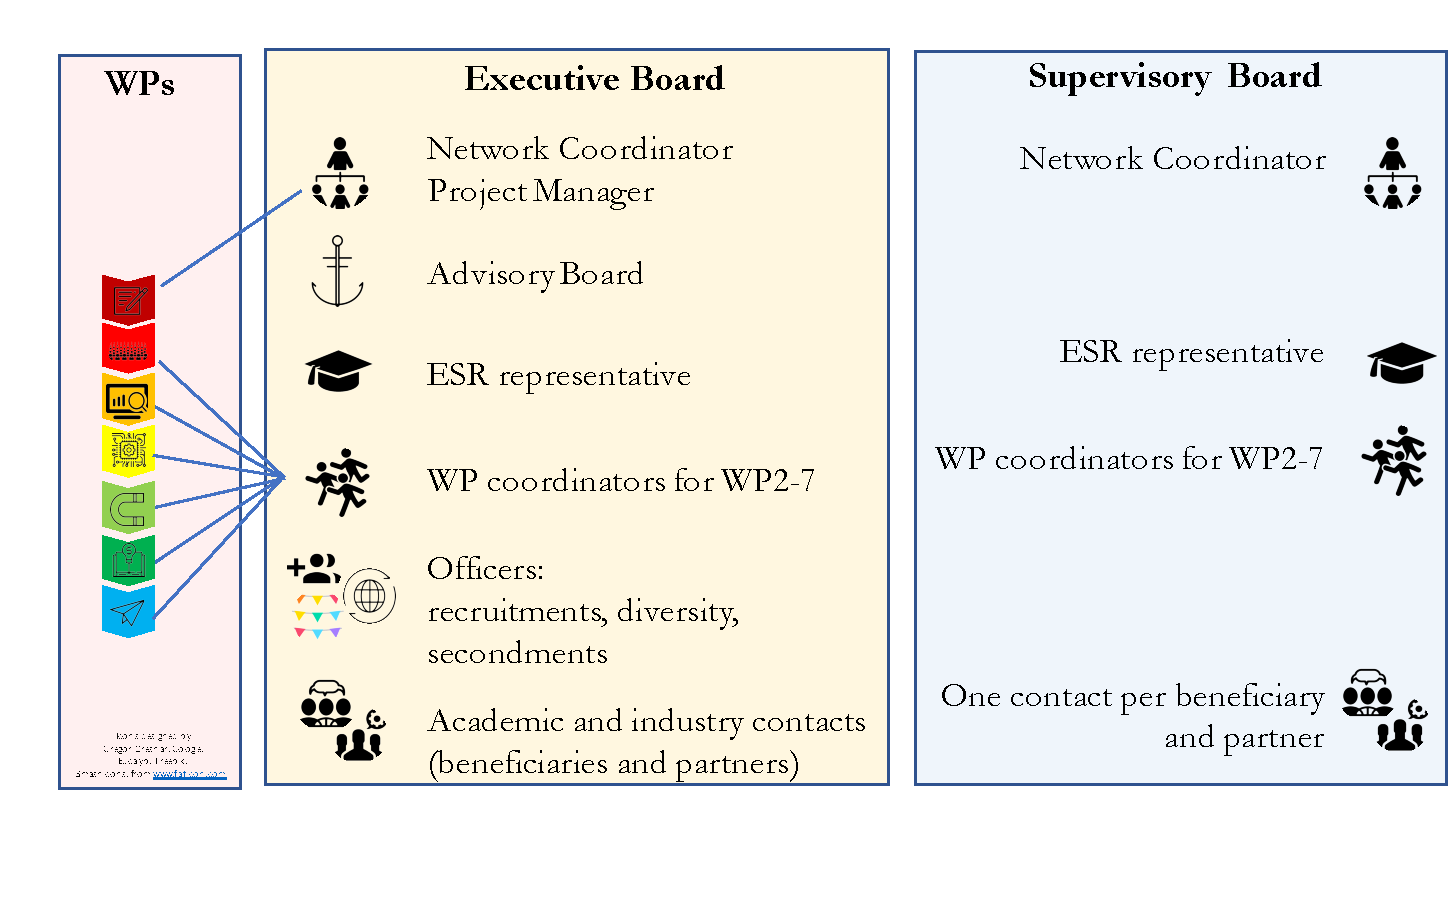
\includegraphics[width=0.7\textwidth]{figs/ManagementStructure.png} %scienceStructure_2.pdf}
%    \vspace{-5mm} 
%%	\caption{Management structure of \acronym.}
%	\label{fig:scienceStructure.pdf}
%%    \vspace{-2mm} 
%%\end{figure}

Official network communication, including decisions taken in EB and SC meetings, will be transmitted on the
existing network e-mail list \texttt{smarthep-participants@cern.ch}. The archives of this mailing list will be available, except in matters requiring non-disclosure. 
In those cases, communication will happen between %by phone and via e-mail involving 
the interested parties according to the regulations of each of the participants involved. 
A "virtual corridor" for the network has already been created at \cern using Mattermost software for rapid, non-official communication and collaboration,
allowing network members to create channels for discussion and effectively share documents, software, and announcements.
%Mattermost allows users to create channels for discussion of given topics through instant messaging, and is integrated with a number of other software package for effectively sharing documents, software and announcements.
%Mattermost effectively builds a virtual corridor in a software system. Mattermost promotes a flat hierarchy between the members of a team or a channel, but it also allows for channels that can only be joined by invitation. The typical use cases here are e.g. the communication among ESRs working on similar projects in geographically different locations, as well as the rapid discussion of network matters among the partners and beneficiaries.  The use of Mattermost to build a virtual corridor is an integral part of this proposal,
%and one that will strenghten collaboration across \acronym researchers for years to come. 

%CD: this is left for the figure
%\vspace{-4mm}
%\begin{wrapfigure}{l}{10cm}
%\begin{center}
%\includegraphics[width=0.75\textwidth]{figs/management2.pdf}
%\caption{\acronym management structure}
%\label{fig:management}
%\end{center}
%\vspace{-5mm}
%\end{wrapfigure}
%\vspace{-4mm}
%
\vspace{-2mm}
\subsubsection{Joint governing structure}% (mandatory for EID and EJD projects)}
\label{sub:jointGoverningStructure}

The EB is the extended project management body of \acronym. 
It is composed of the PC, coordinators of all WPs, a \textbf{student representative} elected from a board that the ESRs will be encouraged to form for their own discussion, three officers responsible for \textbf{recruitment, diversity and secondment} matters, and representatives from each \textbf{academic and industrial beneficiary and partner}. 
The EB is expected to meet via teleconference regularly (e.g. every quarter), as well as on demand.
It is a forum where all WP coordinators and contact persons report on their progress, results or other issues relevant for the Network. 
Action items arising from these reports might be: a communication strategy for a particular publication, the formation of a task force to deal with an identified risk or failure, a new avenue of research or a new product to be developed. 
These meetings will be chaired by the PC and minuted with listed action items. 
Draft minutes will be released shortly after the meeting, and final minutes within a week. 
Each EB meeting will follow up on outstanding action items.
The EB will meet physically during the first days of Network-wide events, and prepare the agenda for the SB meetings. 
The EB will also serve as a point of contact with all \acronym stakeholders, and provides support to the nodes organizing Network-wide events.
Finally, the EB will be able to propose changes to the plans presented in this proposal to the SB.

%CD: this is left for the figure
%\vspace{-4mm}
\begin{wrapfigure}{l}{1.1\textwidth}
%\begin{figure}[!htb]
\begin{center}
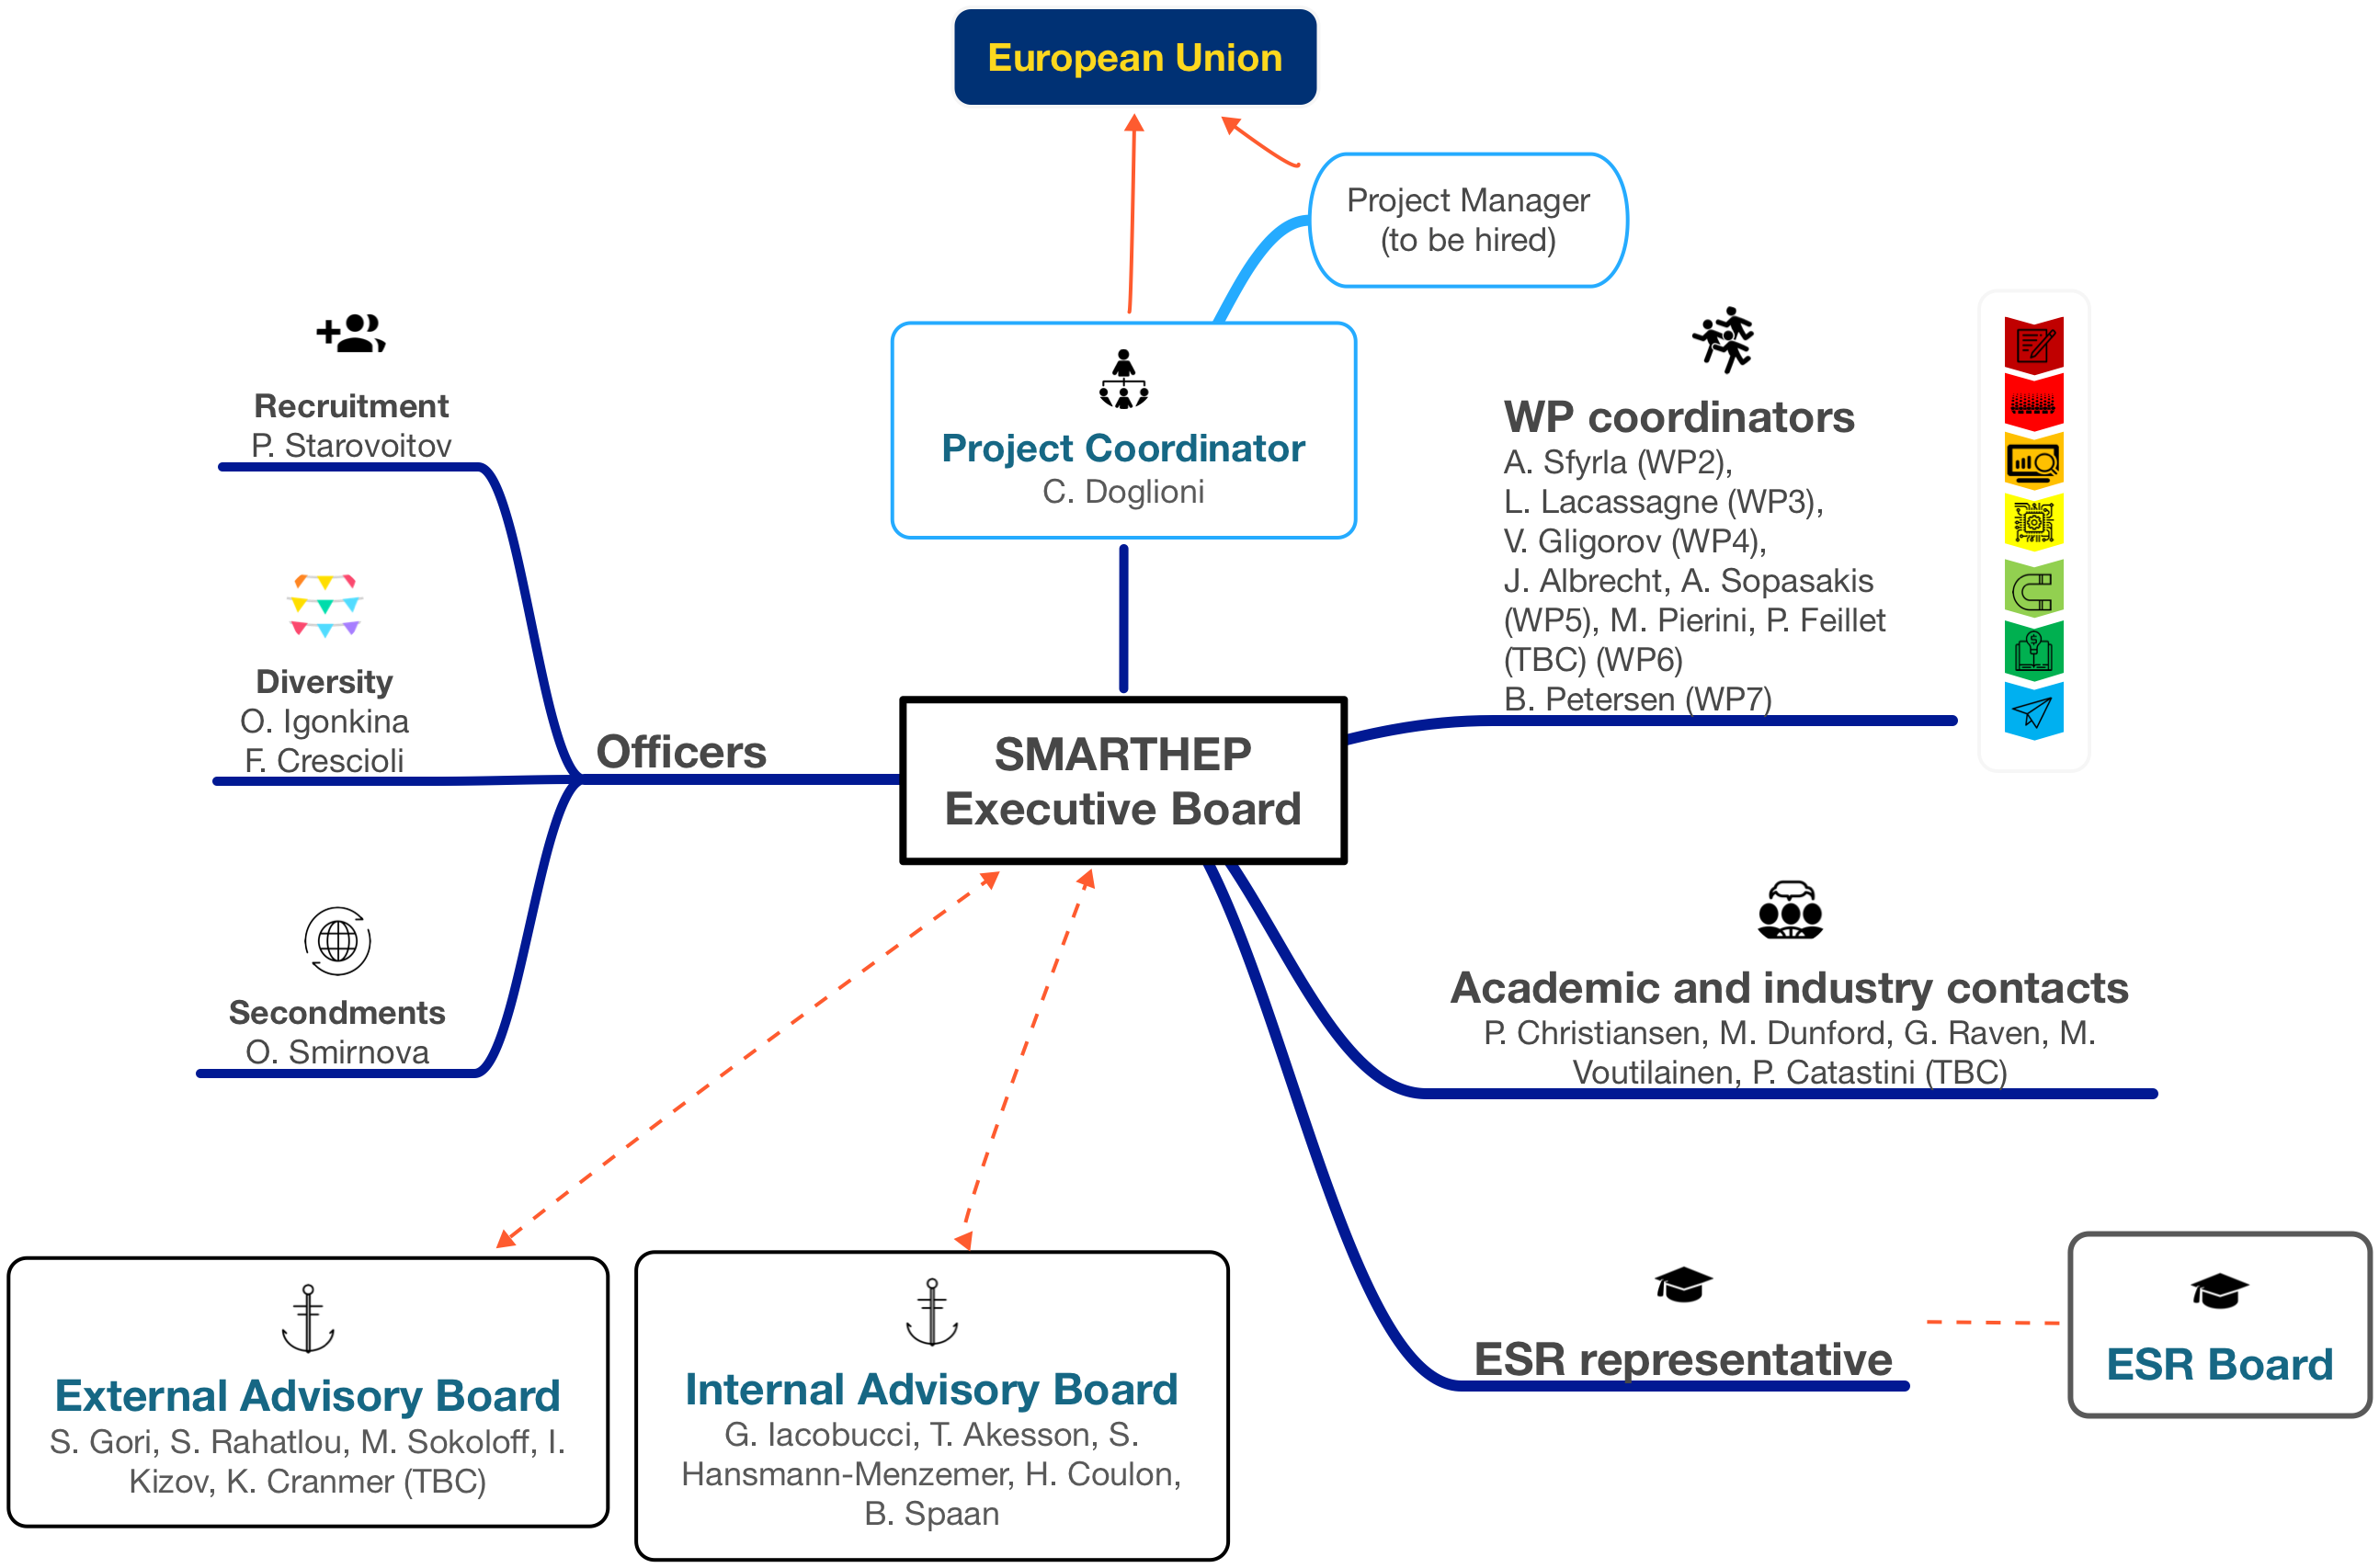
\includegraphics[width=0.7\textwidth]{figs/SMARTHEP_Boards.png} %scienceStructure_2.pdf}
\caption*{Figure 3: \acronym Executive Board (EB)}
\label{fig:management}
\end{center}
\vspace{-5mm}
%\end{figure}
\end{wrapfigure}
%\vspace{-4mm}

The EB will receive advice from the \textbf{Internal and External Advisory Boards}, two groups of senior physicists that will help consolidating the managerial experience of the junior researchers in the network. 
The Internal Advisory Board is composed of senior professors from the beneficiary institutes mentioned in Sec.~\ref{subsub:qual_supervisors}, who have extensive experience in project management and coordination. 
The External Advisory Board is composed of experienced professors that are not employed in beneficiary or partner institutes, who will also participate in the training events. 
It includes Prof. Stefania Gori from UCSC, an expert in theoretical physics phenomenology, Prof. Mike Sokoloff from U. Cincinnati, one of the founding member of the HEP Software Foundation, Prof. Ivan Kisel from FIAS, who is one of the pioneers of many reconstruction methods for particle tracks in high energy physics, Prof. Shahram Rahatlou from University of Rome Sapienza, who has been the CMS Physics Coordinator and Prof. Kyle Cranmer from NYU's center for Data Science, an expert in statistics, machine learning and data preservation. 
The members of this board will act as external observers to the network and offer advice on the impact and dissemination activities as seen from the broader community. 
They will also help resolve conflicts between participants that may arise within the network.
The External and Internal Advisory Board members will be invited to the \acronym yearly meetings. 

\vspace{-2mm}
\subsubsection{Supervisory board}

%\begin{wrapfigure}{l}{1.1\textwidth}
%%\begin{figure}[!htb]
%\begin{center}
%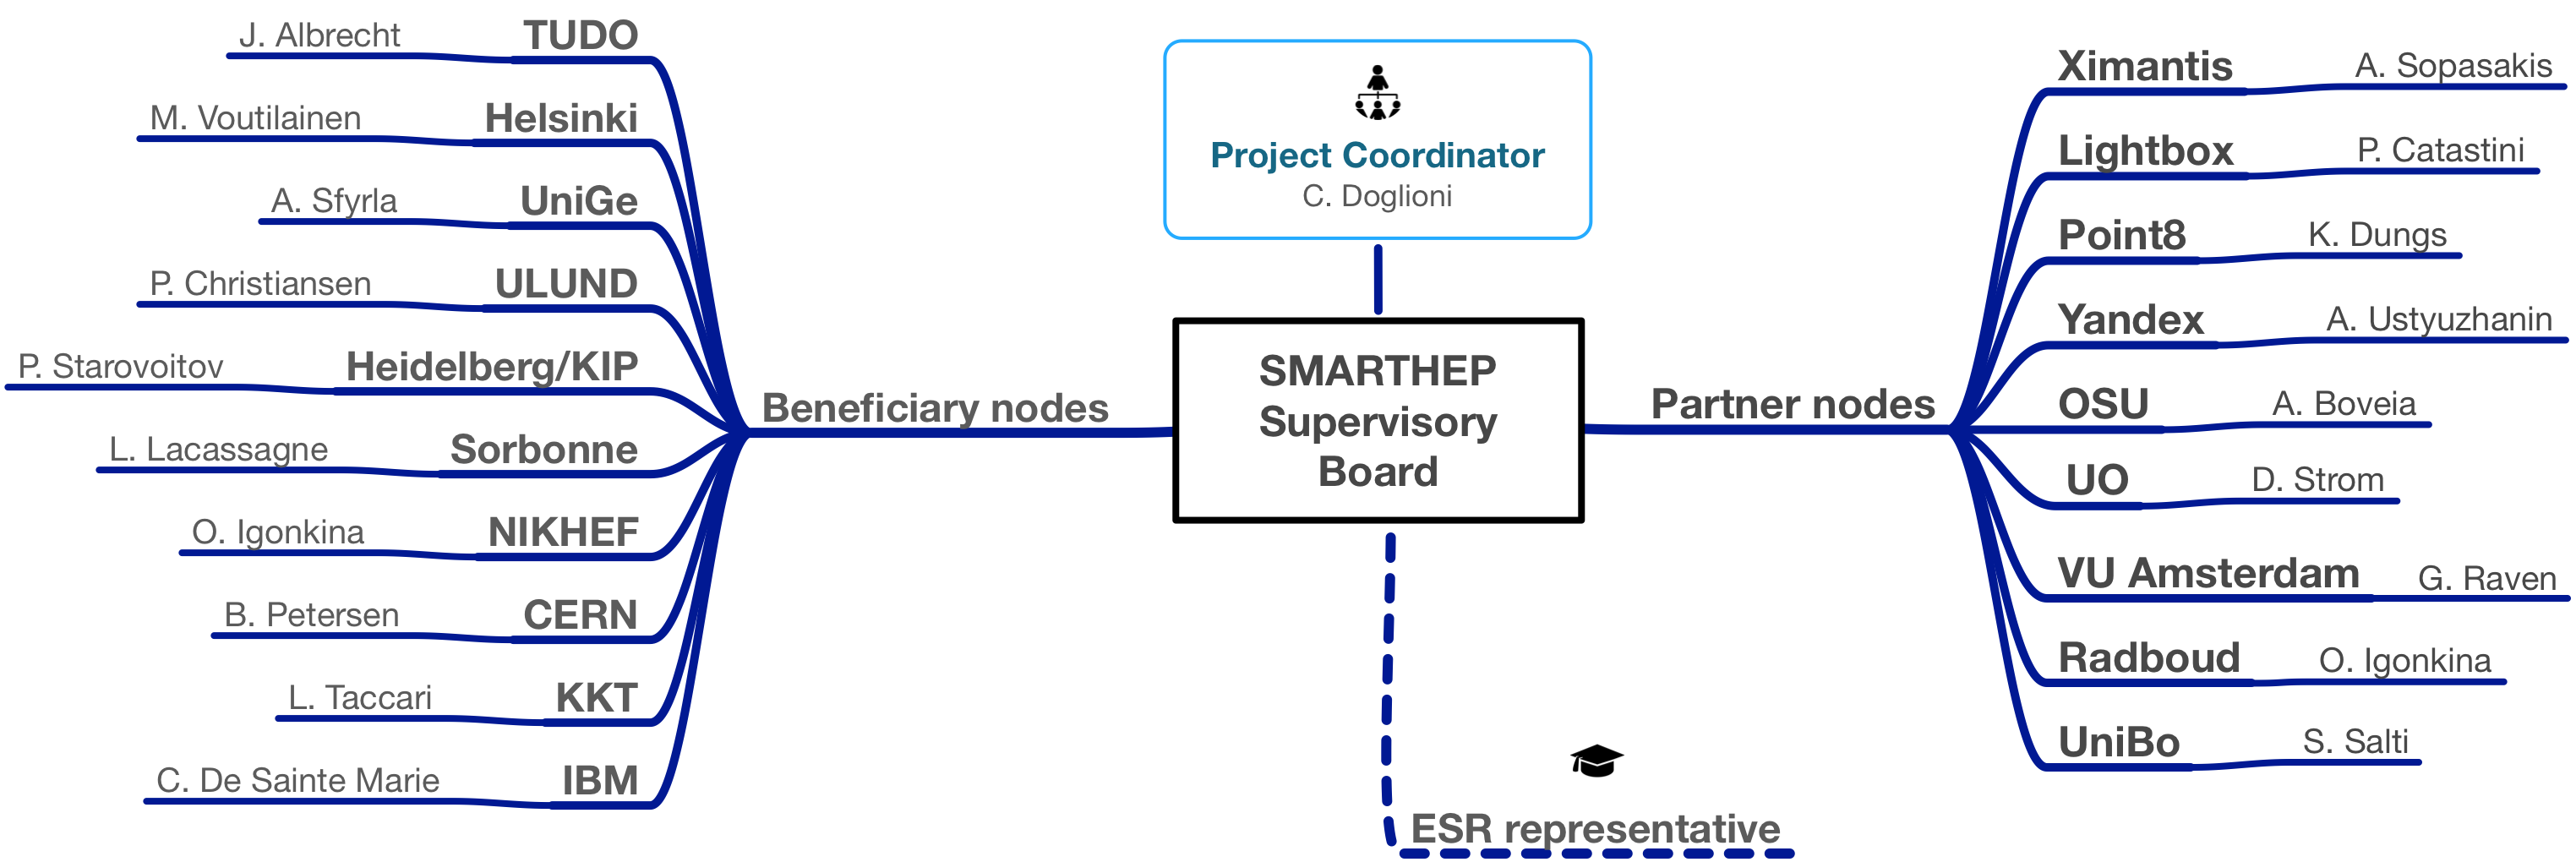
\includegraphics[width=\textwidth]{figs/SMARTHEP_SupervisoryBoard.png} %scienceStructure_2.pdf}
%\caption{\acronym Supervisory Board (SB)}
%\label{fig:management}
%\end{center}
%\vspace{-5mm}
%%\end{figure}
%\end{wrapfigure}
%%\vspace{-4mm}

The SB drafts the CA and is the decision-making body of \acronym in matter of training and project, by majority vote. 
It receives advice and action items from the EB. 
Each \acronym node has a single vote in the SB. They are usually represented through their main contact person as specified in the List of Beneficiaries and List of Partner Organizations Tables.
The student representative will be allowed to participate and vote in the SB, but the SB reserves the right to hold closed meetings in case of items that are critical for one or more ESR (e.g. failed progress, crisis management, scientific misconduct). 
The approval of the PCDPs will not include the ESR vote.
The work plan presented in this proposal will have to be approved by the SB at the Kick-off meeting, to be held during month 2 of the project. 
The SB will also have to approve any measurement proposed by the EB and the PCDP of all the ESRs.
The SB will monitor the progress of the Network, including the quality of training and supervision, and will monitor and take action on scientific misconduct as per the the The European Code of Conduct for Research Integrity\footnote{\url{https://ec.europa.eu/research/participants/data/ref/h2020/other/hi/h2020-ethics_code-of-conduct_en.pdf}}. 
Apart from the Kick-off meeting, the SB will meet yearly in the special Network-Wide events organised by \acronym. 
These meetings will be chaired by the PC.

\vspace{-2mm}
\subsubsection{Recruitment strategy}

%Recruitment
%The following sections of the European Code of Conduct for the Recruitment of Researchers refer specifically to recruitment and selection:
%Employers and/or funders should establish recruitment procedures which are open, efficient, transparent, supportive and internationally 
%comparable, as well as tailored to the type of positions advertised.
%Advertisements should give a broad description of knowledge and competencies required, and should not be so specialised as to discourage 
%suitable applicants. Employers should include a description of the working conditions and entitlements, including career development prospects. 
%Moreover, the time allowed between the advertisement of the vacancy or the call for applications and the deadline for reply should be realistic.
%Selection
%Selection committees should bring together diverse expertise and competences and should have an adequate gender balance and, where appropriate
%and feasible, include members from different sectors (academic and non-academic) and disciplines, including from other countries and with relevant
%experience to assess the candidate. Whenever possible, a wide range of selection practices should be used, such as external expert assessment and
%face-to-face interviews. Members of selection panels should be adequately trained.

\acronym will recruit in compliance with the ``European Code of Conduct for the Recruitment of Researchers''. 
\acronym is committed to appointing the ESRs in a gender unbiased way and candidates will be selected regardless of their race, religion, sexual orientation or disability. 
We are aware that marginalized groups are significantly underrepresented among job applicants and will take proactive steps to advertise \acronym ESR positions among them and highlight their inclusiveness, as discussed in a dedicated section (Sec.~\ref{sub:genderEO}).
\acronym will have a common job advertisement template and a dedicated information webinar for prospective ESRs at the kick-off meeting. Work on the recruitment will start in advance of the CA signature so that all ESRs are recruited by month 8.
Positions will be announced and described in detail on appropriate portals at the national, European, and international level, e.g.
on the Euraxess portal, our web page and social media.

Once recruitment for each node is completed, the corresponding beneficiary main contact will inform the recruitment officer and the relevant WP coordinator(s) and bring the proposal to the EB meeting for approval. 
As part of this approval, the two best-ranked runners-up will be reviewed by the recruitment and diversity officers, as EB members not involved in the original recruitment. 
The goal is to verify that the selection process was unbiased with respect to gender, race, religion, sexual orientation or disability. 
In particular, the review will establish whether there was any unconscious bias on the part of the recruiting panel. 
Starovoitov (\heidelbergshort) will serve as~\textbf{recruitment officer} with a seat in the EB overseeing the recruitment procedure. 

\vspace{-2mm}

\subsubsection{Progress monitoring and evaluation of individual projects}
\label{sub:progressMonitoring}
 
Several progress monitoring and evaluation plans are foreseen:
\begin{itemize}%[topsep=0pt,nosep]
\item A PCDP will be created for each ESR, and approved first by the supervisors and then by the WP coordinator and SB.
\item Supervisors will report on ESR progress to the WP coordinator where the ESR is working, as well as in EB and SB meetings. 
Supervisors will also communicate back the feedback coming from the ESR to the SB.  
\item Each secondment responsible (partner or beneficiary) will write a short progress report of the ESR's work and achievements at the end of the secondment, monitored by the dedicated \textbf{secondment officer} Smirnova (\lundentity). 
Secondments are the basis of lasting relationships between the ESR and the network partners maintained beyond \acronym. 
\item ESRs will present their work in talks and/or posters in the yearly network events, as well as in international conferences when major milestones are reached. 
The ESR presentations and posters will be collected by the \textbf{WP7 responsible} Petersen (\cernentity) on the \acronym website. 
\item Yearly appraisal meetings will be held by beneficiaries, and chaired by the senior members of the institute or university.
\item Each ESR will write half-time and final reports, which will be approved by supervisors and relevant WP coordinators, comparing projects outcomes to the PCDP. 
\end{itemize}
%Apart from these, ESRs will be supported in their work by
Each WP will organise teleconference meetings whose frequency will depend on the size and activities of the group, and will have joint meetings as appropriate.
ESRs will also be encouraged to participate in relevant meetings held by the experimental collaborations and industrial partners.
 
\vspace{-2mm}
\subsubsection{Risk management at consortium level}

Upon its creation and regularly during its meetings, the SB is tasked with creating a detailed Risk Management Plan and bringing it to the attention and approval of the EB. 
A preliminary list of identified risks and proposed mitigation measures relating to the deliverables and milestones defined in Tab.~\ref{tab:DeliverList}~and~\ref{tab:MilesList} are listed the table below.

%\begin{table}
%\small
%\caption{\small Implementation risks\label{tab:RiskManagement}}
\begin{center}\scriptsize
%\begin{center}
%\resizebox {\textwidth }{!}{%
\begin{tabular}{p{10mm}p{65mm}p{5mm}p{85mm}}
\toprule
Risk No. & Description of Risk & WP & Proposed mitigation measures \\
\midrule
R1 (low) & Delays in recruitment & 1 & Announcement of vacancies earlier or soon after signature of grant agreement, awareness of visa issues in consortium, eight month contingency. \\
R2 (medium) & Biases in recruitment & 1 & Targeted advertisements to minority groups, "blind" application process up to interview (only research interests visible up to shortlisting process), cross-check of recruitment approval in EB\\
R3 (low) & Problems in training or outreach event organization & 2, 7 & Two beneficiaries will be assigned to organize a given training or outreach event, 
with the help of the WP responsibles, to have sufficient support and overlap between scientists.\\
R3 (low) & Underperforming ESR & 2-7 & Excellence-based recruitment, continuous monitoring, discussions and feedback, possibility of awarding intermediate degree with one of the beneficiaries (e.g. Licentiate degree) \\
R4 (medium) & Practical difficulties in ESR mobility & 3-6 & Design of academic and industrial secondments requiring maximum 2 long-term stays away from home node, dedicated secondment officer \\
R5 (medium) & Impossible to perform research/secondment (e.g. supervisor changes position or career) & 3-6 & Extra backup projects from each of the partners related to ESR ready during proposal writing stage, more than one PI per beneficiary institute.\\
R6 (low) & Delays in LHC schedule & 5 & Preparation of algorithms and physics searches using simulated data, prototyping research objectives on data already taken.\\
R7 (medium) & Poor performance of planned algorithm/infrastructure & 3,4 & Since some of the techniques used are of a high-risk high-gain nature, this is the most relevant risk for the ESR progress. We will review and downgrade specifications as necessary, with focus on retaining most useful and exploitable characteristics, document work done and reevaluate ESR PCDP by reassigning tasks within the network objectives.\\
\bottomrule
\end{tabular}
%}
\end{center}
%\vspace{-5mm}
%\end{table} 

Risk management will be monitored by each WP coordinator as well as by the diversity, recruitment and secondment officers, following guidelines defined by the SB at the Kick-off meeting and included in the CA.
The WP and research projects are designed such that any potential issue in a single WP or deliverable will not affect the remaining deliverables.
In the case that any major failure in the development of a project is detected, the relevant WP coordinators will inform the EB. 
Together with the ESR, the supervisor(s) and the WP coordinators, the EB will design the best follow-up strategy and will monitor its implementation and outcome.

\subsubsection{Intellectual Property Rights (IPR)}
\label{sec:ipr}

%All ESRs will have access to the background needed to perform their research tasks, but
%the parties will retain IP rights. 
%Preliminary arrangements have been made with \dq and industrial partners to
%respect the commercial exploitation
%of \acronym research, and in general non-HEP algorithms or toolkits will be
%published only following their commercial exploitation. 

\noindent \color{blue}IPR Management during the project.\color{black}
For the success of the project it is essential that all parties agree on explicit rules concerning IP ownership, access rights to any Background and Results for the execution of the project and the protection of intellectual property rights (IPRs) and confidential information before the project starts. 
Therefore, such issues will be addressed in detail within the CA between all project parties. 
Additional industrial partners have granted \acronym access to machines with architectures beyond the state-of-the-art for testing their algorithms, under the agreement that the publication will follow the public release of the machine and that the company producing a given machine is not named until then. 
These machines are hosted at CERN and will be accessible to \acronym researchers. 

\noindent \color{blue}Consortium Agreement. \color{black}
The purpose of the CA is to establish a legal framework for the project in order to provide clear regulations for issues within the consortium related to the work, IP-Ownership, Access Rights to Background and Results and any other matters of the consortium's interest.

\noindent \color{blue}Access Rights to Background and Results. \color{black}
For smooth execution of the project, in the CA the beneficiaries will grant each other and their affiliated companies, royalty-free Access Rights to Background and Results necessary for the execution of the project. 
This will allow the researchers the ability to execute the project to the best of their ability, without being hindered by administrative issues. 
The CA will define further details concerning the Access Rights for Exploitation to Background and Results.

\noindent \color{blue}IP Ownership. \color{black}
Results shall be owned by the project beneficiary carrying out the work leading to such Results. 
It will be agreed among all parties in the Consortium Agreement that the ownership on IP rights will be solely retained at the host beneficiary of the corresponding ESR, when this knowledge is generated during the execution of the project at the host beneficiary. 
For Results created during secondments, specific one-to-one IP rights agreements will be signed on a case-by-case basis.
If any Results are created jointly by at least two parties and it is not possible to distinguish between the contributions of each of the parties, such Results, including inventions and all related patents/patent applications, will be jointly owned by the contributing parties. 
In order to further the competitiveness of the EU market, and to enhance exploitation of the Consortium Results, each contributing party shall have full own freedom of action to exploit the joint IP as it wishes, to further the goals of the consortium. 
To promote this effort the contributing party will have full own consideration regarding their use of such joint Results and will be able to exploit the joint IP without need to account in any way to the other joint contributor(s). 
Further details concerning jointly owned Results, joint inventions and joint patent applications will be addressed in the CA.

\noindent \color{blue}Transfer of Results. \color{black}
As Results are owned by the project parties carrying out the work leading to such Results, each project party shall have the right to transfer Results to their affiliated companies without prior notification to the other project parties, while always protecting and assuring the Access Rights of the other project parties. 
Such use of Results will encourage competitiveness of the EU market by creating broader uses of the Results.

\noindent \color{blue}Open Source. \color{black} 
A central aim of this consortium is to provide benefit to the European community. Some of the project parties may be either using Open Source code in their deliverables or contributing their deliverables to the Open Source communities. 
Details concerning open source code use will be addressed in the CA.

\noindent \color{blue}Website and legacy. \color{black} 
As coordinator node, \lund will maintain the \acronym website and access to the software beyond the end of the project, ensuring that GA signatories retain fair-use access to the deliverables.

%\acronym will release all HEP source code and algorithms developed on the website, on
%\href{http://www.github.com}{github} and similar platforms, and integrate
%them into commonly used DS toolkits such as \tmva\ or \scikit\ where appropriate.
%In the case of ESRs based or seconded at industrial partners, the full
%software toolkits will only be available as part of the developed commercial products,
%while proof-of-concept versions will be released openly.

%These arrangements, together with rest of IPR related aspects,
%will be included in detail in the CA. The CA will also make
%explicit the application of the H2020 IPR rules within the Network.

\vspace{-2mm}
\subsubsection{Gender and equal opportunities aspects}
\label{sub:genderEO}

All members of \acronym believe in fostering a research culture where everyone including marginalized groups feel encouraged to collaborate, and hold this particularly important when training new scientists. 
\acronym will appoint two dedicated~\textbf{equal opportunity officers}, Prof. O. Igonkina and Dr. F. Crescioli, to ensure that during the recruitment and throughout the duration of the action \acronym remains a welcoming research environment and trains both ESRs and its more senior members in matters of inclusion. 

The coordinator of \acronym, as well as more than $30\%$ of the beneficiary contacts, are female scientists\footnote{This is significantly more than the average percentage of women in physics, see \href{https://doi.org/10.1371/journal.pbio.2004956}{The gender gap in science: How long until women are equally represented?}, PLoS Biol 16(4) e2004956}, close to the Commission's goal of 40\% for decision-making panels. 
To mention only examples of the involvements of the \acronym members in increasing diversity in science, Gligorov plays a leading role in promoting diversity and equality within the LHCb collaboration, and authored a statistical analysis of the gender evolution of the LHCb collaboration since its formation, \unigeentity, \cnrsentity, \nikhefentity have been members of the \href{H2020 GENERA network}{https://genera-project.com/index.php/consortium} and \lundentity is an active member of the NORNDIP network financed by Nordforsk. These networks will be a source of support and local training for the ESRs. 

%This directly
%led to the formation of an Early Career, Gender, and Diversity task
%force within the LHCb collaboration,
%with the aim of proactively improving the collaboration's gender balance.

As equal opportunities are a priority for \acronym, we will
actively promote diversity when recruiting the ESRs, while still keeping high scientific
standards throughout the process, according to the European Charter for the Recruitment of Researchers\footnote{
\url{https://cdn2.euraxess.org/sites/default/files/brochures/am509774cee_en_e4.pdf}}. 
In addition to having members of selection panels with
different expertise, gender and personality, \acronym will seek to avoid
biases in our recruitment process through a two-step recruitment policy, with
an explicit focus on the avoidance of unconscious bias.
The \acronym recruitment process will clearly state
the equal opportunities policies in all our recruitment documents,
and our recruitment advertising will prominently
showcase e.g. the female supervisors and SB members of the consortium. 
\acronym are aware of research indicating that minority job applicants
self-select to great extent. \acronym will therefore explicitly (in the job advert)
and proactively encourage applications from female 
and minority candidates by targeting the recruitment advertisement
to specific groups and clubs (e.g. associations of women in physics, 
LGBT at CERN, outreach groups targeting developing countries),
and by highlighting the local diversity and inclusion committees and measures
at the recruiting node in the advert itself. 
The recruitment progress will be reviewed at the
Kick-off meeting of \acronym, and if \acronym find that fewer
than 30\% of applicants at that stage have been women
and/or from minority groups, the SB will be tasked with developing
immediate and explicit corrective measures in order
to encourage more applications from female and minority students.  

All the nodes of the Consortium have a clear commitment to
inclusion and equal opportunities. \acronym will make explicit the
important roles that women and minority groups play in the Network through a section of its web page. 
Female ESRs and ESRs from minority groups will be active in dedicated outreach
activities to show the importance of diversity in science, to act as role models and to demonstrate
in practice the equality of conditions in a welcoming environment in science. 
All \acronym members will be expected to use gender neutral language
in network activities, pay particular attention to desired gender pronouns when referring to ESRs, 
and all \acronym publications will use gender neutral language throughout.
Lectures to avoid unconscious bias will be offered in our Transferable Skills program,
so that our new generation of scientists is educated in the respect, inclusion and
Equal Opportunities policy for all genders.

%\subsubsection{Data Management Plan}

%http://ec.europa.eu/research/participants/data/ref/h2020/grants_manual/hi/oa_pilot/h2020-hi-oa-data-mgt_en.pdf

%\processdelayedfloats
%
%\subsection{Appropriateness of the infrastructure of the participating organizations}
%%%Explain the appropriateness of the infrastructure of each participating organisation, as outlined in Section 5 (Participating Organisations), in light of the tasks allocated to them in the action.
%
All nodes in the consortium have infrastructure appropriate to the tasks
they are responsible for. \lundentity's management is supported by its Research Services, 
which are appropriate for a large university. 
All ESRs will have access to the complete range of \acronym
expertise (Sec.~\ref{ss:competence_44}) and infrastructure (part B2),
and be provided with office space and a laptop for use during \acronym. 
Beneficiaries and the secondment officer will also help with accommodation,
visas and practical issues, making use of the EURAXESS Services for Relocation Assistance. 
Academic support granted to ESRs includes close supervision, mentoring by senior scientists and 
institutional academic literature subscriptions, as well all the facilities supporting research at the nodes. 
All institutes and research laboratories have software divisions with excellent computing
capabilities and infrastructure, including rack-mounted
servers and large data storage systems, locally and on the Worldwide Computing Grid. 

As detailed for each node in part B2, \acronym participants
contribute with the specific facilities and equipment required for the successful completion of the WPs.
In particular, partners hosting secondments involving GPUs and hybrid architectures host those on their premises
and ESRs will be able to use them during the secondment and remotely on demand. 
Moreover, a number of industrial entities have agreed with Prof. Lacassagne that \ESRg
will be able to make use of beyond-state-of-the-art machines to test algorithms developed
throughout the duration of \acronym, and that \ESRg will
be able to disseminate results in open access journals as soon as
the machines become public, within the course of their PhD project. 

\subsection{Competences, experience and complementarity of the participating organisations and their commitment to the program}
\label{ss:competence_44}

\subsubsection{Consortium composition and exploitation of participating organisations' complementarities}
\label{sub:composition}

The academic beneficiaries and partners of \acronym are the pioneers and experts of RTA in each of the LHC experiments. 
They have a strong background in the physics topics that are the focus of the network, as the network includes 5 ERC grantees and scientists who have covered and are covering positions of responsibilities within large international collaborations as detailed in Secs.~\ref{subsub:qual_supervisors} and part B2.
%Even though the network is mostly composed and led by early-career, emergent researchers, they all have extensive experience in student supervision and research. 
Researchers in \acronym have already been successfully collaborating within their experiments on complementary topics. 
Scientists in \nikhefentity, \cnrsentity, \dortmundentity (LHCb), \oregonentity, \ohioentity, \lundentity, \heidelbergentity (ATLAS), \helsinkientity (ATLAS)  and \lundentity (ALICE) lead the trigger and RTA techniques developments for each of the collaborations. 
Expertise in ML is given by \pointeightentity, \unigeentity, by LHCb researcher Ustyuzhanin from the Yandex School of Computing and \yandexentity.  

The synergy in the RTA physics program of \acronym is cross-collaboration, with researchers from \nikhefentity, \cnrsentity and \dortmundentity researching LFV/LFU in ATLAS and LHCb, researchers from \unigeentity, \cernentity, \helsinkientity, \heidelbergentity, \ seek new physics through Higgs and dark sector particles in ATLAS and CMS, while \lundentity and \helsinkientity precisely measure the Standard Model of particle physics in CMS and ALICE. 
%The network also benefits from theory expertise with the affiliated theorists of Dark Matter and LFV/LFU from \ohioentity and \cincinnatientity. 
%The combination of WP4, led by one researcher per collaboration, and WP7 led by \cernentity
%will ensure that the results of physics research are disseminated and communicated effectively. 
%Hybrid architectures (WP5, led by L. Lacassagne of \cnrsentity) are another necessary ingredient of RTA,
%as software-only solutions on standard CPUs are not sufficiently fast for the purposes of HEP and industry alike. 

Software and machine-learning experts from \pointeightentity, \ximantisentity, \heidelberginstrumentsentity, \cernentity and \ibmentity as well as experts in hybrid infrastructures in \pisaentity, \cnrsentity, \fleetmaticsentity and \lightboxentity provide the complementary tools to develop efficient solutions to both industry and research problems, and in the case of the industrial partners, practical implementations with a commercial value. 
%The combination of Machine Learning, novel data analysis techniques and hybrid architectures are applied to commercial examples of real-time data analysis. 
%All commercial partners have a concrete interest in these techniques. 

The status of \cernentity as an international collaboration that hosts all HEP experiments provides the ideal framework in which to exploit the research complementarity within the network and support its 
advancements beyond the state of the art. An example is the recently Internet-of-Things Openlab effort at CERN\footnote{First workshop of Internet-of-Things at CERN, \url{https://indico.cern.ch/event/669690/overview}, Nov 2017} whose organizers informally agreed to support this network through a half-day training and presentation day. 
The participation of all LHC collaborations to \acronym and the explicit support of the HEP Software Foundation (see letter of support) offers a unique chance to form lasting collaborations and shape the future data taking strategies of LHC experiments and beyond, building from the  results obtained in \acronym.  

%%%%Non-academic

%As explained in Sec.~\ref{sec:supervision}, all the beneficiaries 
%%are either able to enrol the ESRs in their doctoral school programs
%%or have established co-supervision arrangements 
%%for the ESRs to obtain their  in another institution within the Network. 
%training in industry and knowledge transfer at \dq [mention heidelberg school]. 
%In particular the dedicated and hands-on \cern HEP schools and the [school of data analysis and ML]
%will complement the more traditional university-based lectures of other academic nodes, while
%\dq 
%%, \technopolis 
%and the partner companies will provide training which will greatly increase the employability of
%the ESRs. %Summer schools, academic lecture series as well as the full spectrum
%%of training courses offered by the \acronym participants will be open to all ESRs.



%%explain the compatibility and coherence between the tasks attributed to each
%beneficiary/partner organisation in the action, including in light of their experience;


%
%The research synergies and complementarities
%between the \acronym participants have been described in detail in Sec.~\ref{sec:synergy}.
%
%
%The non-academic beneficiaries and partners have been chosen for their active involvement in research
%and development related to optimising decisions with a commercial purpose, 
%leading to a common interest in RTA shared with the \acronym participants, 
%as detailed in Sec.~\ref{sec:EXCELLENCE}. 
%
%%Of particular importance are the training courses and secondments opportunities
%%offered by our industrial partners, which will give first-hand insight
%%and hands-on experience in the commercial world.
%
%TO BE FILLED AFTER TRAINING PART IS DONE
%

\subsubsection{Commitment of beneficiaries and partner organisations to the program}
%(for partner organisations, please see also sections 5 and 7).

While the majority of the \acronym academic participants are already successfully collaborating in research projects within the LHC experiments, this is the first network that including all major LHC experiment that will consistently advance RTA through Machine Learning and hybrid architectures for modern particle physics experiments and industry alike. 
In-person meetings for the members of the \acronym network have been taking place since May 2017\footnote{\href{https://indico.lucas.lu.se/event/656/}{SMARTHEP kickoff meeting}, supported by the Grace och Philip Sandbloms Fund}. A number of subsequent meetings have taken place, including the RAPID2018 workshop (Sec.~\ref{sec:synergy}), and culminated in a three-day workshop dedicated to the preparation and collaborative editing of this ITN \footnote{\href{https://indico.lucas.lu.se/event/656/}{SMARTHEP kickoff meeting}, supported by Lund Research Services}. 
It is clear from the enthusiasm and participation of all members, as well as from the support offered to this network by \lundentity, that all \acronym participants are fully committed to this project.

High quality education of students in large-scale international projects is already an essential part of the mission of the universities and research labs in \acronym. 
\acronym will greatly strengthen and extend their capacities to carry out these activities, by dedicating a significant fraction of research and supervision time to \acronym activities (see node descriptions in part B2).
All industrial nodes are committed to \acronym, to benefit from the experience in RTA of LHC experts, to foster connections to the academic world and to expand their activities. 
The industry parties have a strong motivation to participate in cutting edge developments and the subsequent transfer of the technologies to new commercial applications.
\acronym partners will not only contribute training to the network, but will also benefit in their own research and commercial objectives through the secondment projects of the ESRs. 

The relations between the nodes, established starting from the preparation of the project will last even beyond \acronym: 
to organize post-graduate recruitment events for companies in the network that specifically target \acronym ESRs after the completion of their PhD and to continue the series of training events and offer them to the European graduate student community.  
%\acronym participants therefore have already established long-lasting
%and fruitful professional relations, marked by mutual respect and trust.
%In short, there is no doubt that all participants in \acronym
%will show the highest level of commitment to the research program. 


%i) Funding of non-associated third countries (if applicable): Only entities from EU Member States, from Horizon 2020 Associated Countries or from countries listed in General Annex A to the Work program are automatically eligible for EU funding. If one or more of the beneficiaries requesting EU funding is based in a country that is not automatically eligible for such funding, the application shall explain in terms of the objectives of the action why such funding would be essential. Only in exceptional cases will these organisations receive EU funding.16 The same applies for international organisations other than IEIO.

%ii) Partner organisations: The role of partner organisations and their active contribution to the research and training activities should be described. A letter of commitment shall also be provided in section 7 (included within the PDF file, but outside the page limit).

%\processdelayedfloats
%%%Explain the appropriateness of the infrastructure of each participating organisation, as outlined in Section 5 (Participating Organisations), in light of the tasks allocated to them in the action.
%
%\FloatBarrier
%\end{document}
%%
%
%\clearpage
%%%
%{\color{red} Stop page count (max 30 pages sections 1-3)}
%%%
%\section*{GANTT CHART}
%\label{sec:gantt}
%%%%\section{GANTT CHART}
%\vspace{2cm}
\clearpage
%\phantomsection
%\stepcounter{section}
%\addcontentsline{toc}{section}{\protect\numberline{\thesection}GANTT CHART}
\captionsetup[figure]{justification=justified,singlelinecheck=false}
\begin{figure}[p]
\vspace{-5mm}
\begin{flushleft}
\caption*{\textbf{\large 4 GANTT CHART\vspace{-5mm}}
\label{sec:gantt}}
\end{flushleft}
\begin{center}
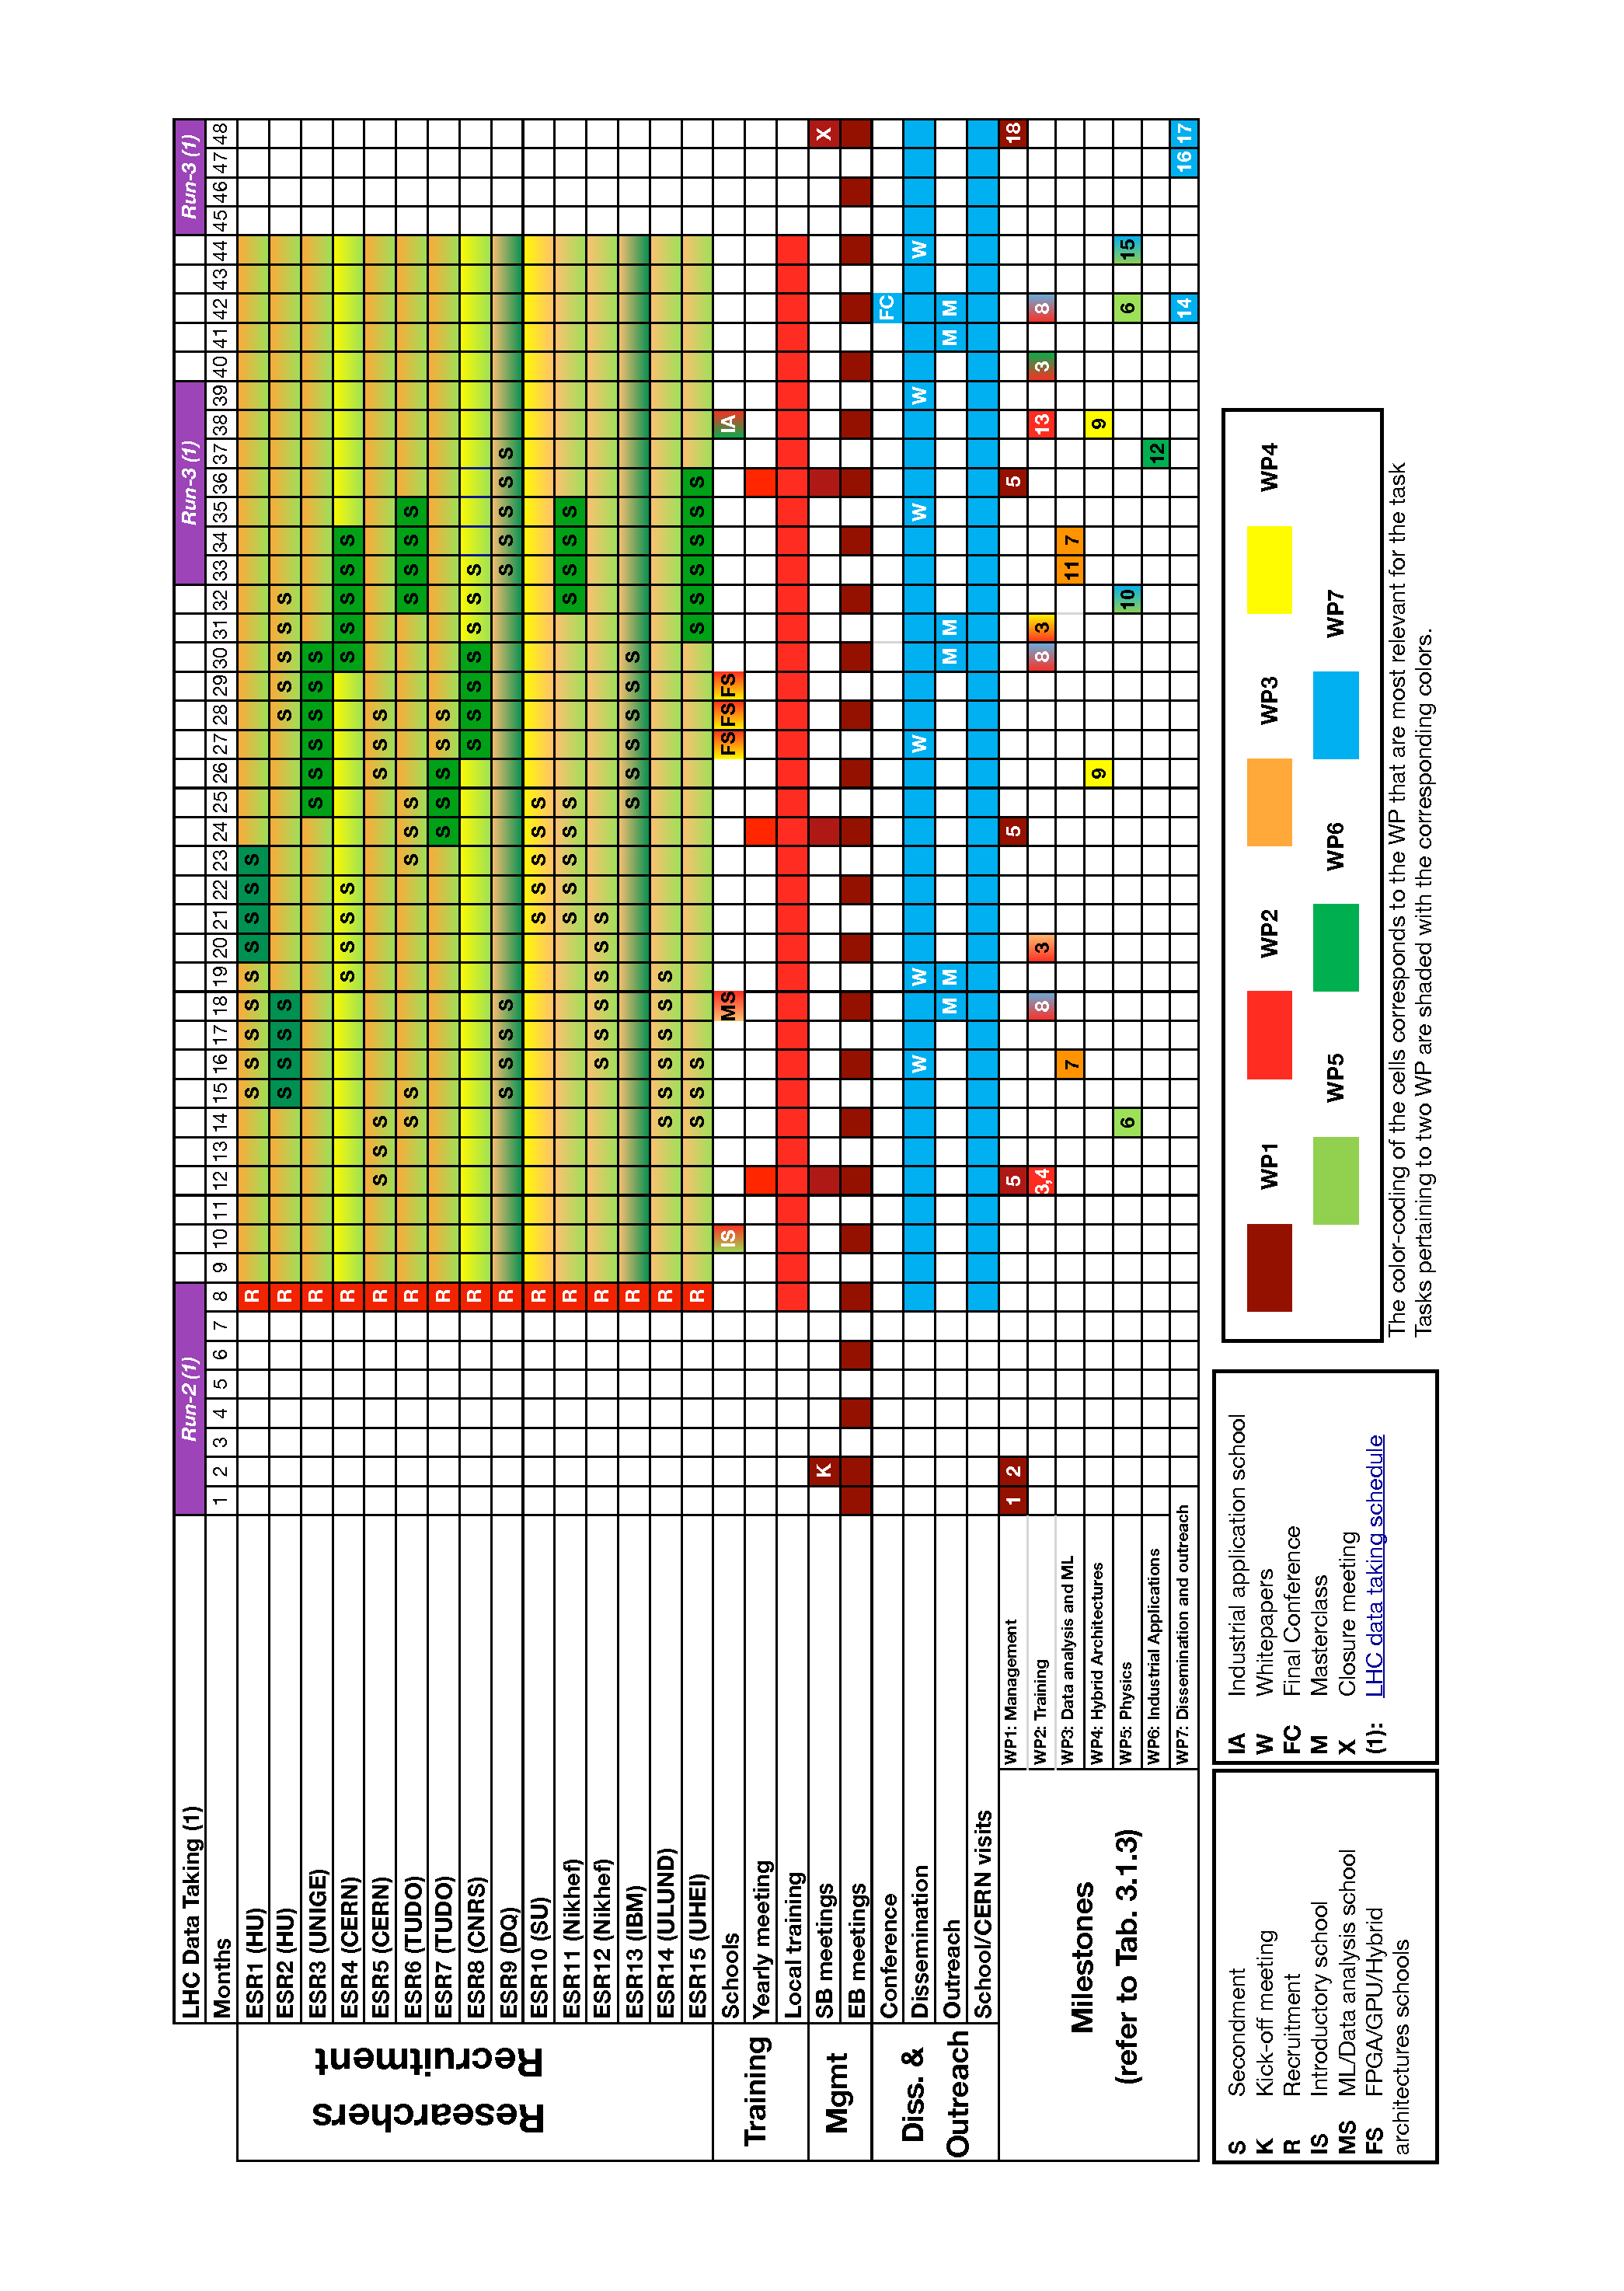
\includegraphics[width=0.835\paperwidth]{figs/gantt_v2.pdf}
\end{center}
\end{figure}
\clearpage\newpage

%%%%\addcontentsline{toc}{section}{GANTT CHART}
%%%%NB: The schedule of the project should be in terms of number of months elapsed from the start.
%%%\section{GANTT CHART}
%\vspace{2cm}
\clearpage
%\phantomsection
%\stepcounter{section}
%\addcontentsline{toc}{section}{\protect\numberline{\thesection}GANTT CHART}
\captionsetup[figure]{justification=justified,singlelinecheck=false}
\begin{figure}[p]
\vspace{-5mm}
\begin{flushleft}
\caption*{\textbf{\large 4 GANTT CHART\vspace{-5mm}}
\label{sec:gantt}}
\end{flushleft}
\begin{center}
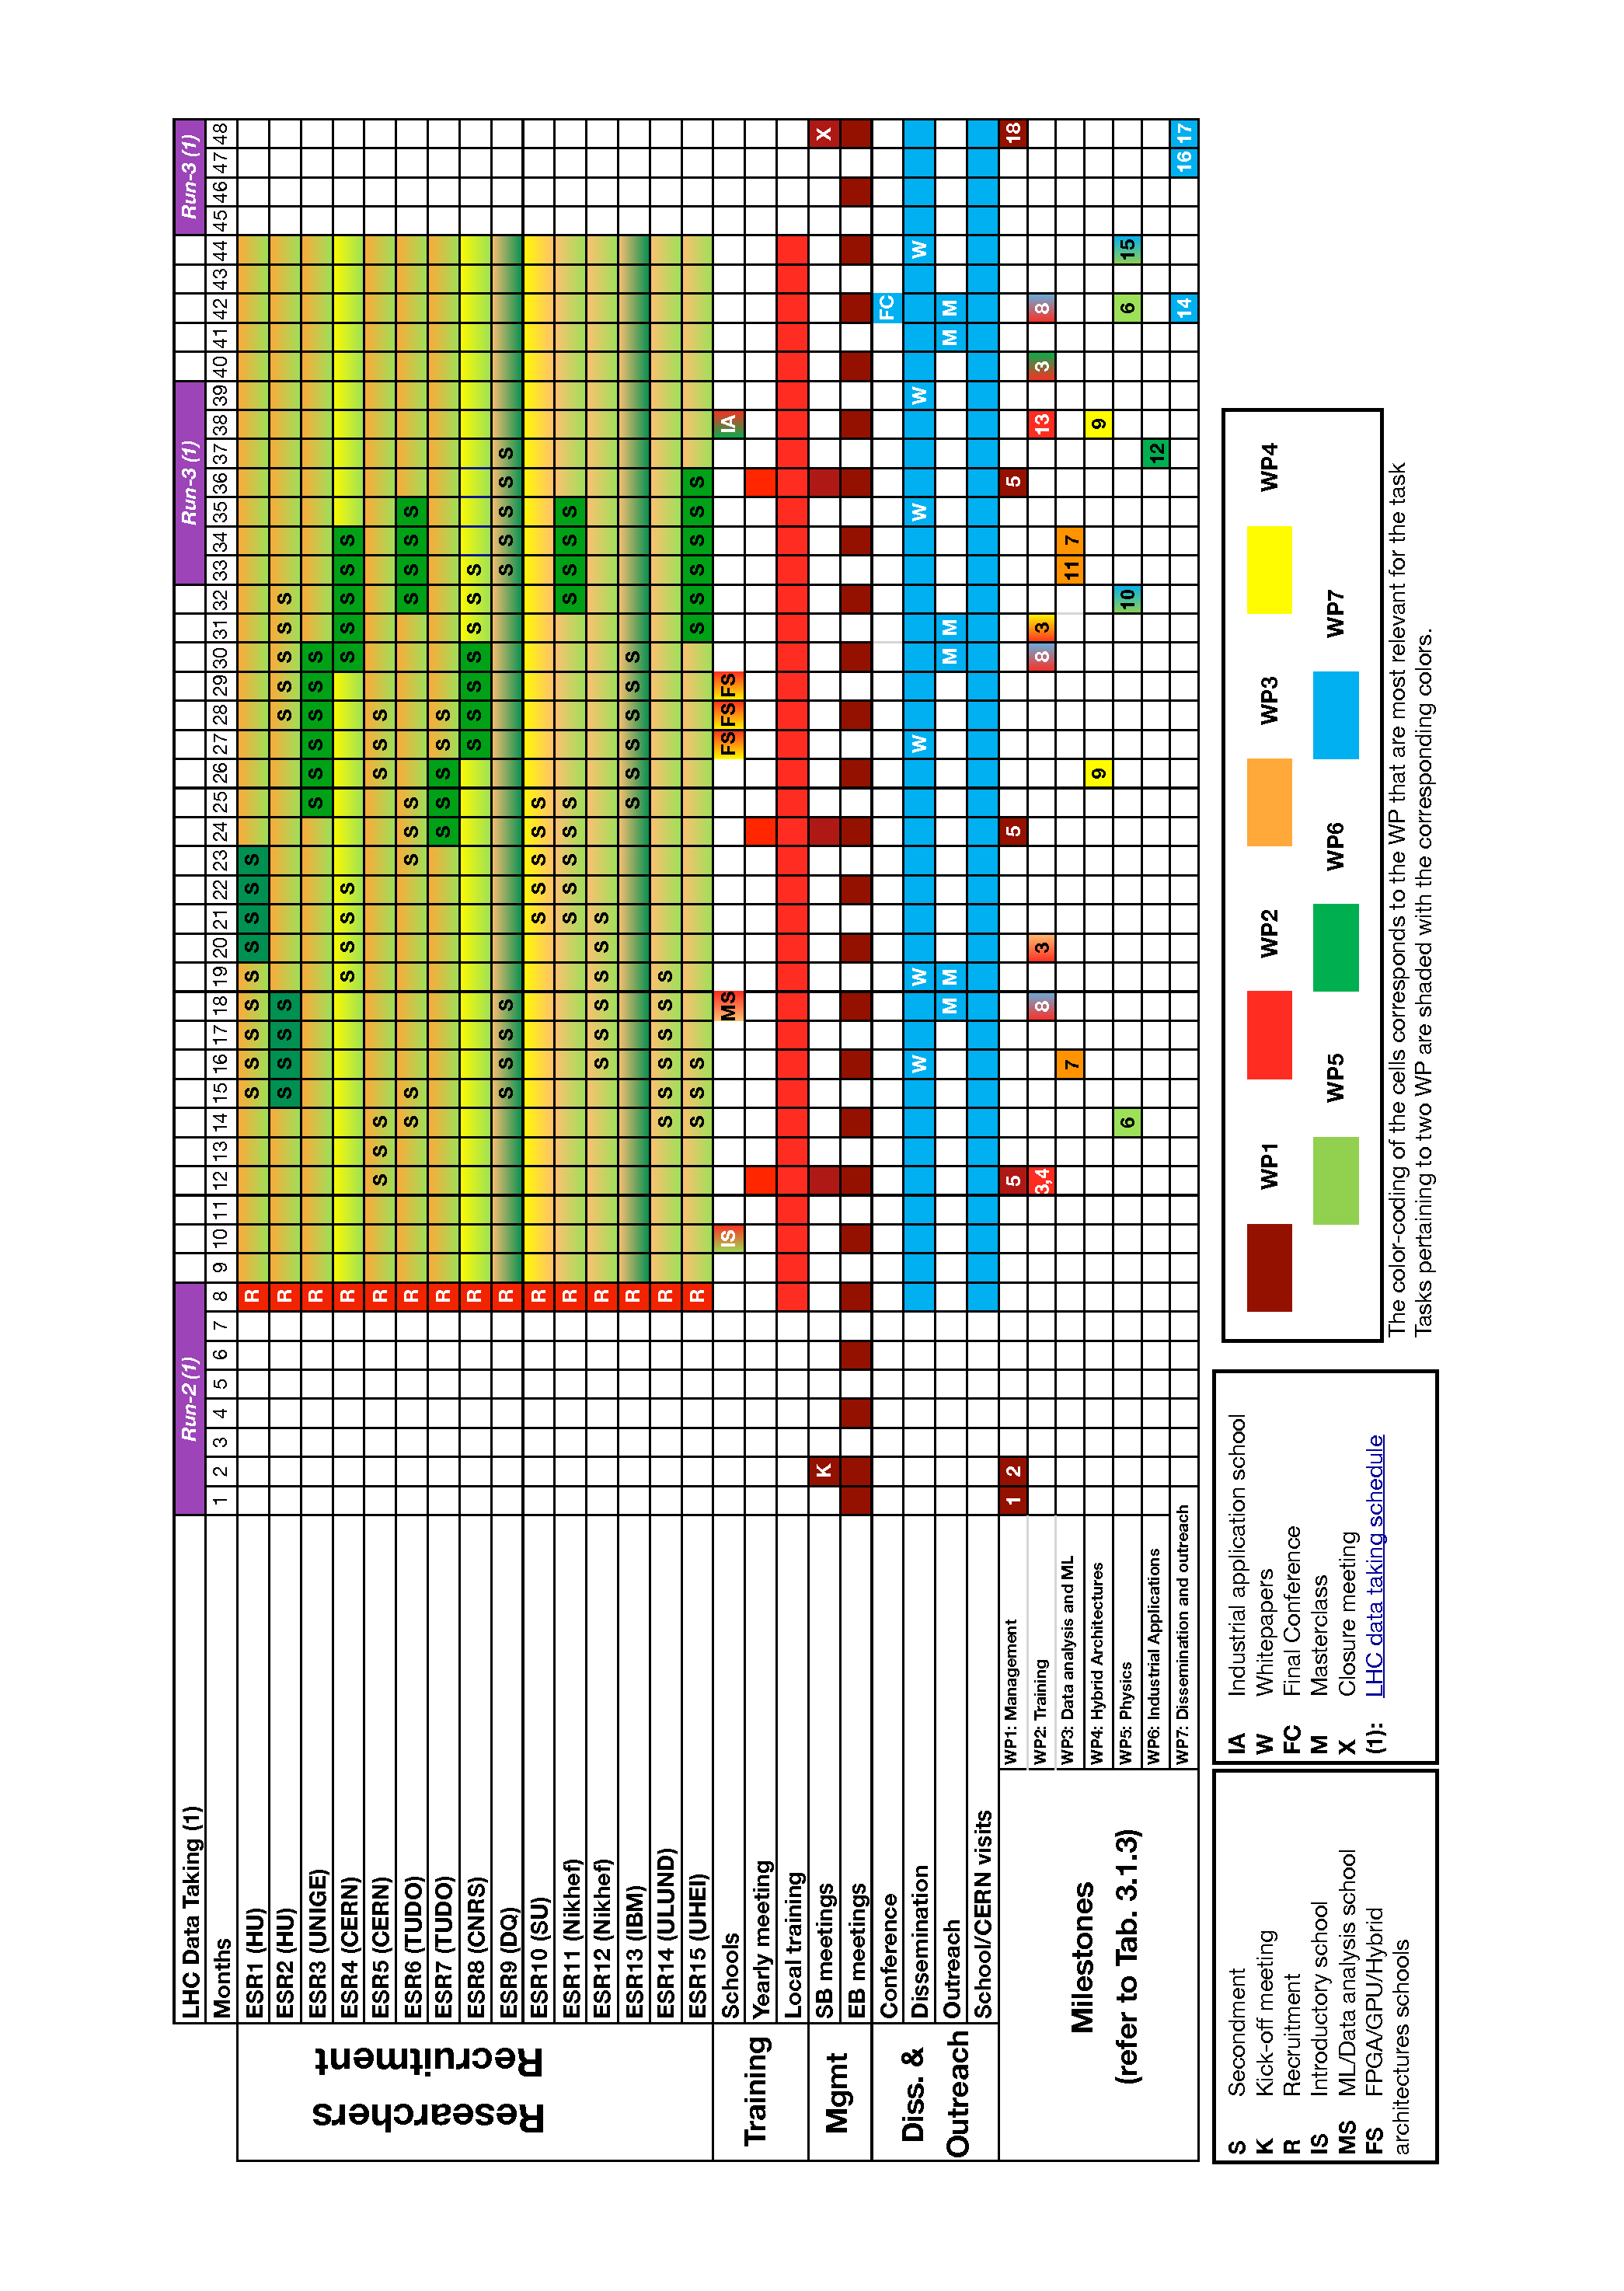
\includegraphics[width=0.835\paperwidth]{figs/gantt_v2.pdf}
\end{center}
\end{figure}
\clearpage\newpage

%{	\centering 
%	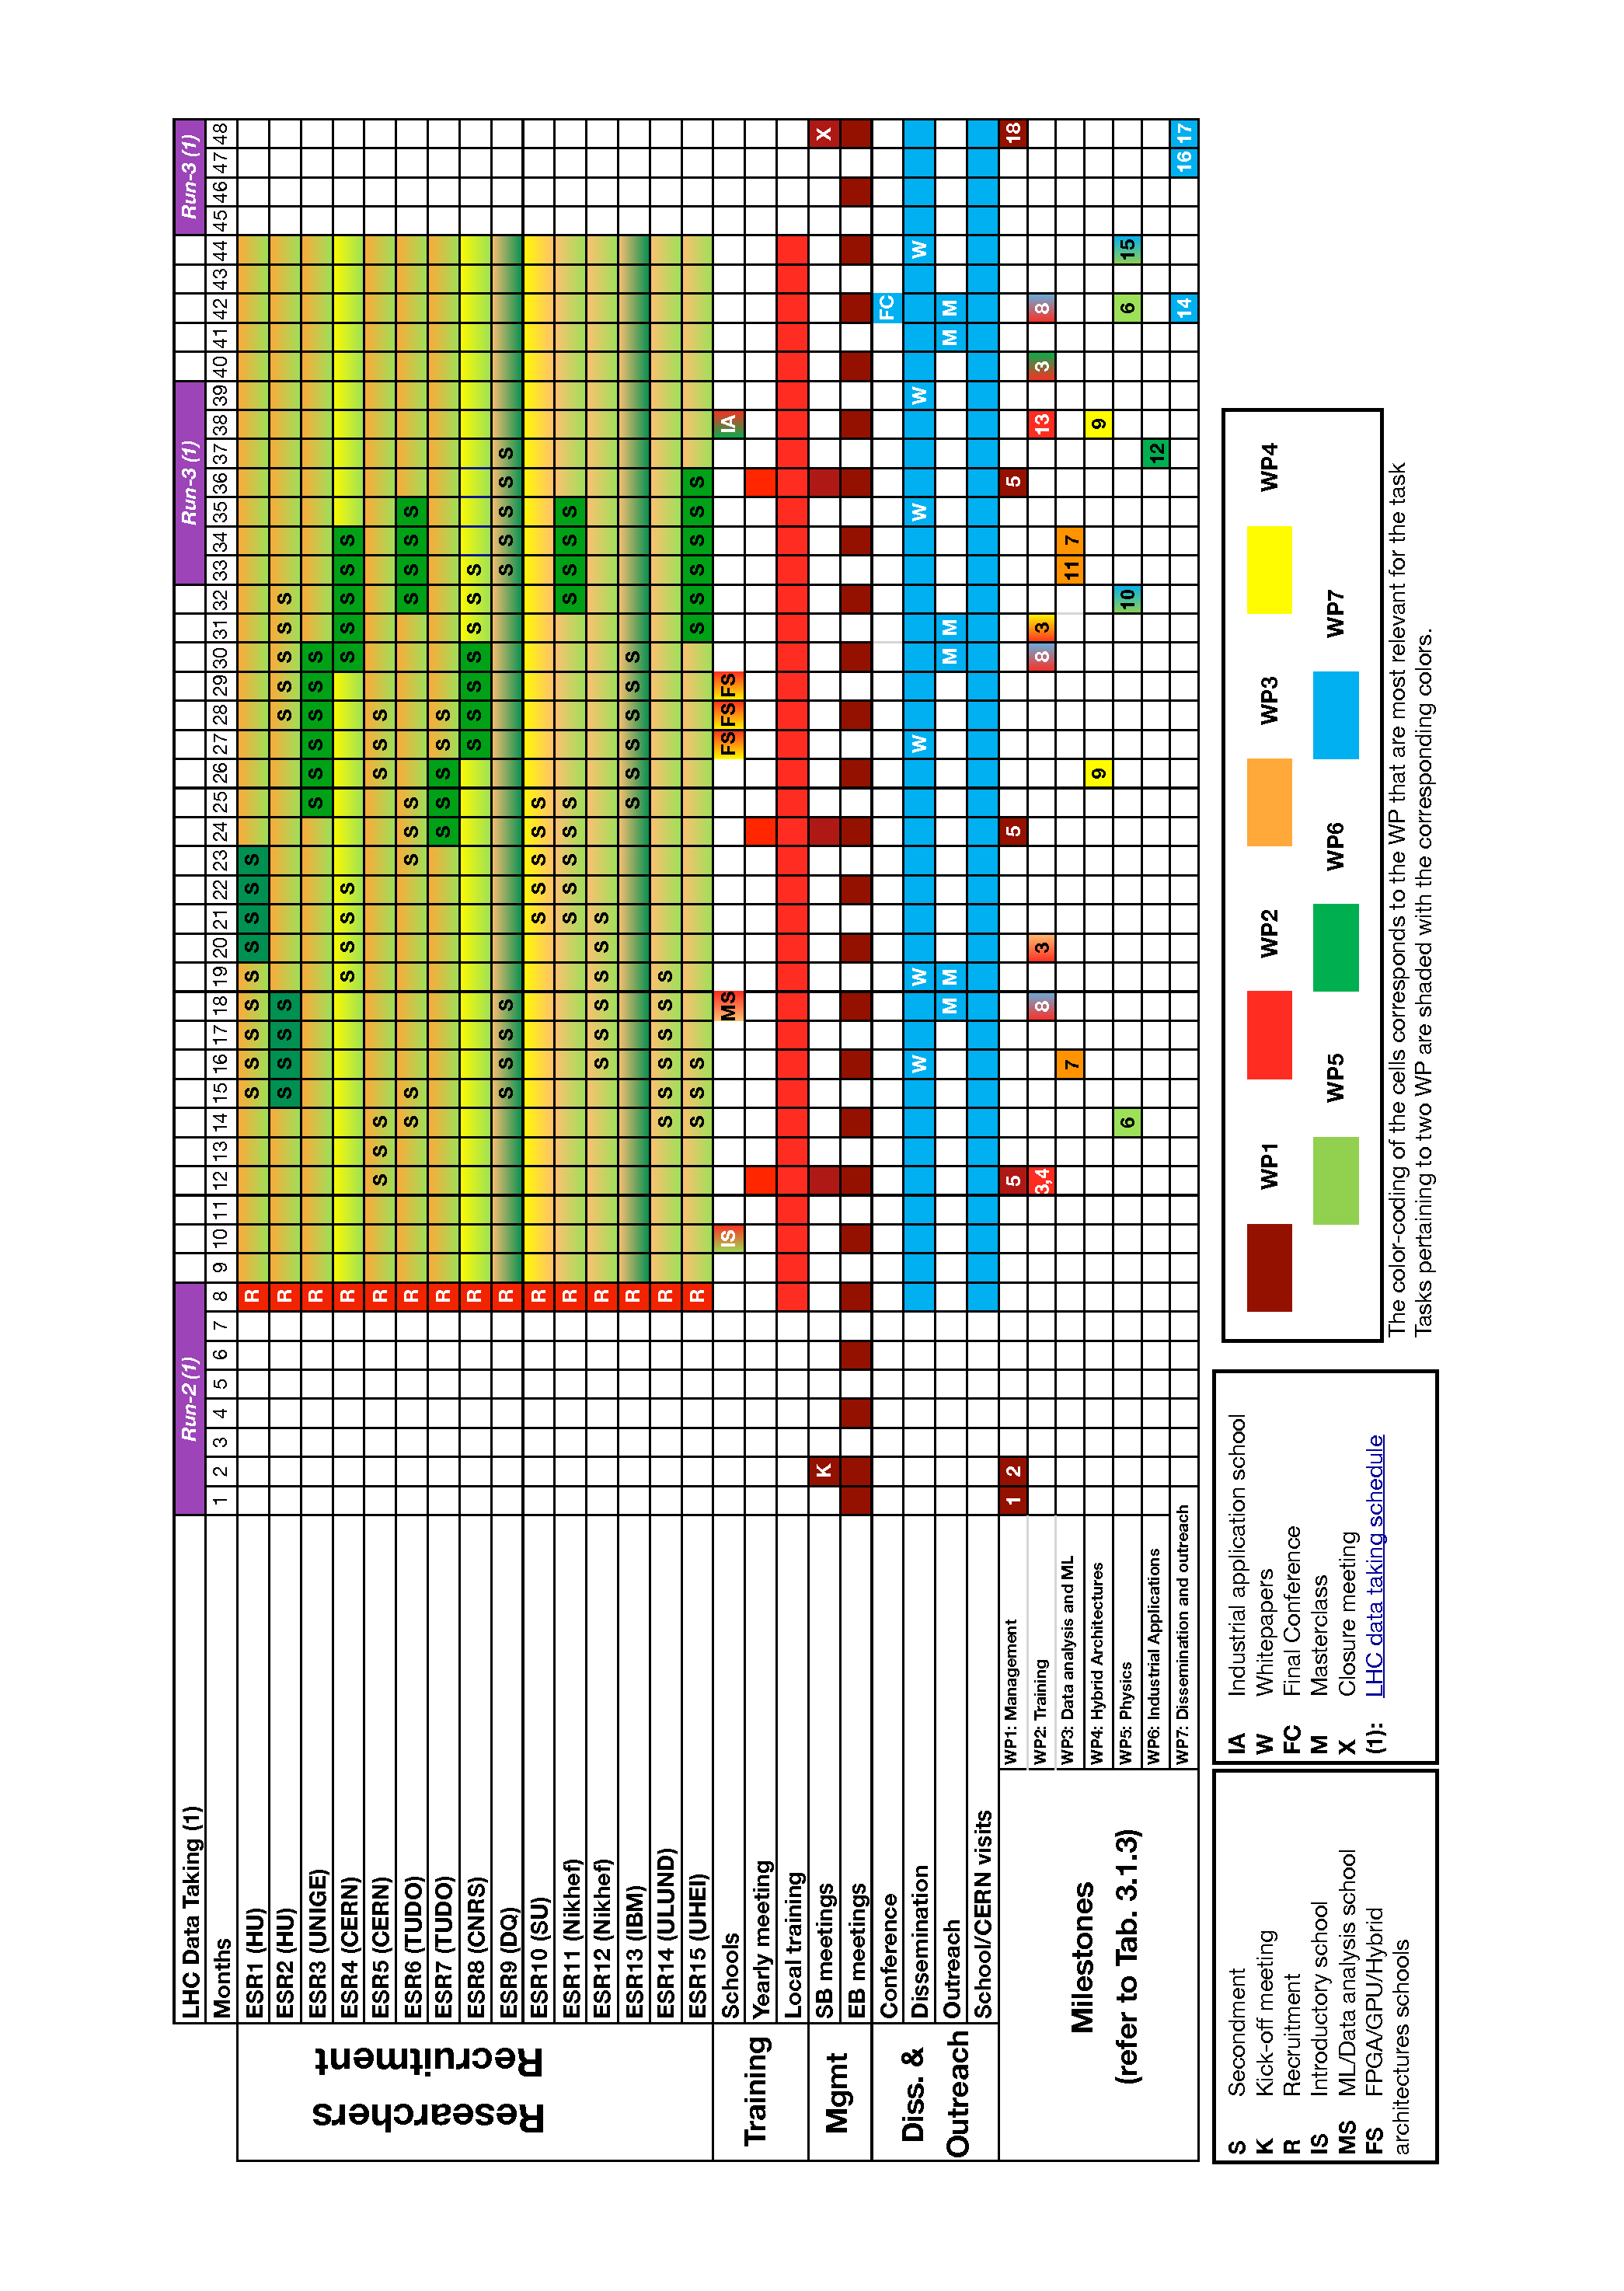
\includegraphics[width=0.9\textwidth]{figs/gantt_v2}
%}
%
%
%%%
\section*{CAPACITIES OF THE PARTICIPATING ORGANISATIONS}
%All organisations (whether beneficiaries or partner organisations) must complete the appropriate table below. Complete one table of maximum one page per beneficiary and half a page per partner organisation (minimum font size: 9). 
%
%For beneficiaries:
%
%Beneficiary Legal Name:
%General Description:
%Short description of the activities relevant to the action
%Role and Commitment of key persons (including supervisors):
%Including names, title and the intended extent of involvement in the action - in percentage of full-time employment - of the key scientific staff who will be involved in the research, training and supervision
%Key Research Facilities, Infrastructure and Equipment:
%Outline the key facilities and infrastructure available and demonstrate that each team has sufficient capacity to host and/or offer a suitable environment for supervising the research and training of the recruited Early-Stage Researchers
%Status of Research Premises:
%Please explain the status of the beneficiary's research facilities ? i.e. are they owned by the beneficiary or rented by it? Are its research premises wholly independent from other beneficiaries and/or partner organisations in the consortium?
%Previous Involvement in Research and Training Programmes: 
%Detail any relevant EU, national or international research and training actions/projects in which the beneficiary has previously participated
%Current Involvement in Research and Training Programmes:
%Detail any relevant EU, national or international research and training actions/projects in which the beneficiary is currently participating
%Relevant Publications and/or Research / Innovation Product (Max 5)
%
%For partner organisations:
%
%Partner Organisation Legal Name: 
%General description
%Key Persons and Expertise
%Key Research Facilities, Infrastructure and Equipment
%Previous and Current Involvement in Research and Training Programmes 
%Relevant Publications and/or Research / Innovation Product (Max. 3)


\begin{center}
%\resizebox{\textwidth}{!}{%
\footnotesize
\begin{tabular}{@{}p{25mm}|p{190mm}@{}}
\toprule
\multicolumn{2}{c}{\large\textbf{Beneficiary: \lundlong}}\tabularnewline\hline
\pbox{8cm}{\Tstrut General\\Description\Bstrut} & %
\pbox{19cm}{\Tstrut \lundlong was founded in 1666,
% and for a number of years has been ranked among the world’s top 100 universities~\footnote{See \href{http://www.lunduniversity.lu.se/about/about-lund-university/university-world-rankings}{http://www.lunduniversity.lu.se/about/about-lund-university/university-world-rankings}}. 
the University has 42\,000 students and more than 7\,500 staff based in Lund, Helsingborg and Malmoe. 
The Faculty of Science conducts research and education within Biology, Astronomy, Physics, Geosciences, Chemistry, Mathematics and
Environmental Sciences. 
%The Faculty is organized into ten departments, gathered in the
%northern campus area. 
The Faculty has approximately 1\,900 students, 330 PhD students and 700 employees. 
The Department of Physics is with a staff of about 350 scientists and educators one of the largest departments within \lundlong. 
There are seven research divisions and a number of research centers within the department. 
The research activities at the department cover a broad spectrum of modern physics.
% For more information, see \url{www.fysik.lu.se/english}.  
\Bstrut}\tabularnewline\hline

\pbox{8cm}{\Tstrut Role and\\Commitment\\of Key persons} & %
{\vspace{-8mm}
\begin{enumerate}%[topsep=0pt,itemsep=-2pt,leftmargin=*]
\item Dr.~Caterina Doglioni, physics, senior associate lecturer, 
%convener of ATLAS Exotics jet+X physics group (2012-2014), 
convener of HEP Software Foundation Trigger and Reconstruction working group (2018-present), LHC Physics Center Dark Matter working group organizer (2015-2018), ATLAS Astroparticle forum (2014-2016), 
receiver of ERC Starting Grant 2015 (DARKJETS, Grant Agreement no. 679305) and Swedish Research Council Starting (2015) and Project (2018) grants. 
Expertise in jet reconstruction, dark matter, triggering, real-time analysis in ATLAS.
\textbf{Role:} Project Coordinator, supervisor of \ESRj, tutoring of seconded students. Commitment: 30\%.
\item Dr.~Peter Christiansen, physics, professor of experimental particle physics, expert in real-time detector reconstruction and analysis for the ALICE experiment. Receiver of Wallenberg Project grant CLASH and of Swedish Research Council Project grant (2017). 
\textbf{Role:} supervisor of \ESRk, lectures and organization of training, commitment: 20\%. 
\item Dr.~Oxana Smirnova, physics, associate professor of experimental particle physics, computing grid and distributed data analysis expert, Grid Architect in 2002-2003 and Sweden's representative in the International Computing Board. Receiver of Swedish Research Council Project grant (2017). 
\textbf{Role:} tutoring of seconded students, commitment: 20\%.
%\vspace{-\belowdisplayskip}
\end{enumerate}} \tabularnewline\hline

\pbox{8cm}{\Tstrut Key Research\\Facilities,\\Infrastructure\\and Equipment} & %
\pbox{19cm}{\Tstrut Lund University is active with a strong, long-term contribution to the ATLAS Experiment and the ALICE Experiment.
This ITN fits well the research interests and existing efforts in the group: an ongoing ERC StG, held by Doglioni, includes real-time data analyses
in searches for new physics in jet final states.   
The opportunities for collaboration within the group are strong as the ESRs in this project extend the research program, and there is sufficient room for a clearly defined, original line of research for the students in this project.   
The expertise that can be found in the theoretical physics department of Lund is also invaluable for all physics searches and measurements
in this ITN: the \textsc{Pythia} event generator developed in Lund is the most used for the simulation of both signal and background 
events for jet searches in the ATLAS Collaboration. 
In \lundlong, the ESRs will also benefit from the use of a computing cluster connected to the NorduGrid network, which can be used for fast and efficient data analysis. 
The combination of a strong understanding of the theoretical issues for the comparison of collider Dark Matter searches and a hands-on experience with LHC data will be conducive to developments and collaboration between the beneficiaries of this project, other Swedish Universities contributing to Dark Matter searches within ATLAS and the Swedish NORDITA Dark Matter program that can be undertaken during and beyond the time frame of this project. 
Furthermore, there are two major research facilities in Lund: MAX IV, a world-leading synchrotron radiation laboratory which has opened in 2016, and the European Spallation Source (ESS), a European facility that will host the most powerful neutron source. 
We plan to exploit existing collaborations with researchers at ESS and MAX IV though on the topics within this ITN, allowing cross-pollination of ideas from the visiting researchers and industrial partners that will be beneficial for the training of students resident or seconded in Lund within and beyond the network.
} \tabularnewline\hline
%
\multicolumn{2}{l}{\hspace{-1ex}Independent \Tstrut  research premises\Bstrut: yes}\tabularnewline\hline
\pbox{8cm}{\Tstrut Past \& current\\involvement\\in Research and\\Training\\Programmes} & 
\pbox{19cm}{\Tstrut \lundlong has been and is currently involved in several EU funded projects, in a number of disciplines, hosting several ERC (starting and advanced) grants. 
One of them is the Doglioni's DARKJETS ERC, concerning discovery strategies for Dark Matter and other new phenomena at the LHC, which has a connection to this project. 
Lund particle physics is directly involved in the INSIGHTS ITN (GA No.765710), concerning statistics for physics and society, with which \acronym plans to collaborate in co-organizing a training event. 
Even though Doglioni was the original \lundentity responsible for INSIGHTS, the role of local node coordinator has been assigned to Else Lytken, allowing Doglioni to have time to be PC of \acronym if funded. 
We also plan to collaborate with the~\href{http://www.montecarlonet.org/}{MCNet ETN}, that has a long tradition in Lund.} \tabularnewline\hline\Tstrut
\pbox{8cm}{\Tstrut Relevant\\Publications} &%
{\vspace{-3mm}
\begin{description}%[topsep=0pt,itemsep=-2pt,leftmargin=*]

\item [O. Buchmueller, C. Doglioni and L.T. Wang] Search for dark matter at colliders. Nature Physics 13, 217223 (2017). 
%
\item [ATLAS Collaboration, C. Doglioni and M. Dunford as editor and A. Boveia as analysis contact] Search for low-mass dijet resonances using trigger-level jets with the ATLAS detector in pp collisions at $\sqrt{s}$=13 TeV, Phys. Rev. Lett. 121, 081801 (2018). 
%%Performance of the ATLAS Trigger System in 2015. Eur.Phys.J. C77 (2017) no.5, 317
%
\item [ALICE Collaboration] The ALICE TPC, a large 3-dimensional tracking device with fast readout for ultra-high multiplicity events. Nucl. Instrum. Meth. A 622, 316 (2010) 1
%
\item [ALICE Collaboration] Centrality dependence of the nuclear modification factor of charged pions, kaons, and protons in Pb-Pb collisions at $\sqrt{s_NN}$=2.76 TeV. Phys. Rev. C 93, 034913 (2016)
%
%%Search for new phenomena in dijet mass and angular distributions from $pp$ collisions at  $\sqrt{s}=13$~TeV with the ATLAS detector
%%[ATLAS Collaboration]. Physics Letters B 754 (2016) 302-322
%
%%\item (2015) Search for new phenomena in the dijet mass distribution using $pp$ collision data at $\sqrt{s}=8$~TeV with the ATLAS detector
%%[ATLAS Collaboration]. Phys.Rev. D91 (2015) 052007

\item [O. Smirnova] Current Grid operation and future role of the Grid, in Proceedings of CHEP 2012, J. Phys.: Conf. Ser. 396 042055 (2013)

%Published in \href{http://10.1140/epjc/s10052-014-3190-y}{}. 

\end{description}}\tabularnewline\bottomrule

\end{tabular}
%}%
\end{center}

%\begin{center}
\resizebox{\textwidth}{!}{%
\begin{tabular}{@{}p{25mm}|p{190mm}@{}}
\toprule
\multicolumn{2}{c}{\large\textbf{Beneficiary: \cern}}\tabularnewline\hline
\pbox{8cm}{\Tstrut General\\Description\Bstrut} & %
\pbox{19cm}{\Tstrut 
\cern is an International European Organization and is the worlds largest particle physics centre, providing technologically-advanced facilities for particle physics. 
CERN has 22 member states. 
Close to 13,000 scientists from 650 institutes worldwide are involved in the research and technology programme. 
CERN's mission is focused on 4 topics: research, technology, collaboration and education, including a long and strong training tradition via the Fellows, Associates and Students programmes. 
It has its own Learning and Development service providing almost 14,000 person days of technical management, communication, academic, safety and language training per year. 
The Large Hadron Collider, the largest and most powerful human-made particle collider, is located at CERN, together with its four main experiments: ALICE, ATLAS, CMS and LHCb. 
Researchers from all four collaborations, who spearheaded real-time analysis in their own experiments, are involved in \acronym.  
CERN hosts the largest particle accelerator in the world, the Large Hadron Collider (LHC), which generates data rates of over 100~Exabytes per year.  
CERN's aims include education and it offers a number of educational and training  programmes to students and teachers, as well as playing a leading role in the International Masterclass programme. 
\Bstrut}\tabularnewline\hline
\pbox{8cm}{\Tstrut Role and\\Commitment\\of Key persons} & %
{\vspace{-8mm}
\begin{enumerate}%[topsep=0pt,itemsep=-2pt,leftmargin=*]
\item Dr.~Monica Pepe-Altarelli is a senior physicist at CERN and a member of the LHCb collaboration in which she held several positions of responsibility.
She is Vice-President Elected at Large of the Executive Council of the International Union of Pure and Applied Science  (\href{http://iupap.org/executive-council-and-commission-chairs/executive-council-officers-2017-2020/}{IUPAP}) as well as Associate Member Delegate to the EPS Council for the period April 2017-2021. She has expertise in data analysis in the NA32, ALEPH and LHCb collaborations.
% Dr.~Monica Pepe-Altarelli, CERN staff. She has been LHCb deputy spokesperson and member of LHCb's Gender, Equality, and Diversity task force. 
%She has also been Vice-President Elected at Large of the Executive Council of the International Union of Pure and Applied Science 
%(\href{http://iupap.org/about-us/executive-council/executive-council-officers-2014-2017/}{IUPAP}).
% Expertise in data analysis in NA32, ALEPH and LHCb.
Role: supervision and mentoring of visiting students, lectures. 
Committment: 10\%.
\item Dr. Rosen Matev, CERN LD staff, expertise in software and trigger design and maintenance, RTA, luminosity measurements. 
Has co-supervised three PhD and a MSc student, currently co-supervising a CERN doctoral student. 
Received LHCb Early Career Scientist award, shared with four other colleagues, on the Run II software trigger. 
Role: co-supervisor of \ESRd.
Commitment: 20\%.
\item  Dr. Benjamin Couturier, CERN staff. After graduating from the Ecole Superieure d'Electricite (Supelec) and the University of Paris-Sud in 1996, Benjamin Couturier has been working as Software Engineer and Software Architect for various companies before joining CERN. He is now part of the team developing the software framework used to process and analyze data from the LHCb experiment at CERN.
Role: co-supervisor of \ESRg and \ESRi, lectures, non-academic training.
Commitment: 20\%.
\item Dr. Andrey Ustyuzhanin is the head of Yandex-CERN joint projects as well as the head of Laboratory of Methods for Big Data Analysis at National Research University Higher School of Economics. 
%His team participates in LHCb and SHiP (Search for Hidden Particles). 
He is an expert in machine learning and gives regular lectures on Machine Learning applied to High Energy Physics. % at the Yandex School of Data Analysis. 
Role: lectures, data challenge responsible, non-academic training.
Commitment: 10\%. 
\item Dr. Brian Petersen is a CERN staff scientist, and a member of the ATLAS collaboration. 
He has been the coordinator of the ATLAS trigger group of the ATLAS upgrade physics group.
He has supervised multiple CERN fellows and was chair of the 2017 CERN-Fermilab Hadron Collider Physics Summer School.
Role: supervisor of \ESRc and seconded students, lectures, commitment: 20\%
\item Dr.~Maurizio Pierini is the coordinator of the Physics Performances and Dataset (PPD) area in CMS, and the initiator of the Data Scouting analyses at the trigger level in CMS. 
He is a CERN staff scientist, and a LPC Distinguished Researcher of the Fermilab Physics Center.  
Role: co-supervisor of \ESRa, lectures.
Commitment: 15\%
\item Dr. Ruben Shahoyan is an expert on software and coordinates the reconstruction and calibration activities within the  O2 software project for ALICE Run3/4 upgrade. 
He coordinates the ALICE upgrade activity on calibration and reconstruction, and has played a critical role in calibrating the space point distortions of the existing Time Projection Chamber.
Role: co-supervisor of \ESRk, lectures.
Commitment: 15\%
\vspace{-3mm}
\end{enumerate}} \tabularnewline\hline
\pbox{8cm}{\Tstrut Key Research\\Facilities,\\Infrastructure\\ and Equipment} & %
\pbox{19cm}{\Tstrut World-class accelerator facilities: PS / SPS / LHC complexes. 
In-house engineering/technology/detector physics groups, prototyping, material science services, mechanical and electronics workshop, etc.
Due to its position as a focal point for research into elementary particle physics and associated technologies, CERN has state-of-the-art technological infrastructure and equipment. 
This spans a very large range of facilities such as accelerators and particle detectors, a forefront informatics backbone including Grid developments, state-of-the-art laboratories for mechanical, electronic, microelectronic and optoelectronic engineering and large cryogenics installations.
%In addition to standard office space with fibre-optic network connectivity and a library with access to over 2000 journals relevant to HEP and DS, CERN provides extensive support and infrastructure for both data analysis and computing.
%This includes a 100 node computing cluster and 2~Tb of disk space for each researcher's own work.
%In addition ESRs will have access to a dedicated cluster of around 10 nodes composed of the latest available GPU processors, and a second dedicated cluster of around 10 nodes composed of the latest available CPU 
ESRs will have access to dedicated clusters with the latest available GPU and CPU processors.
} \tabularnewline\hline
\multicolumn{2}{l}{\hspace{-1ex}Independent \Tstrut research premises\Bstrut: Yes
}\tabularnewline\hline
\pbox{8cm}{\Tstrut Past \& current\\involvement\\in Research and\\Training\\Programmes\Bstrut} & 
\pbox{19cm}{\Tstrut 
CERN has a learning and development programme offering about 15 Academic Training courses per year on subjects ranging from theoretical and experimental particle physics, to advances in technologies, computing and engineering. 
%It offers summer programmes for students and high school teachers, including dedicated physics and computing summer schools, as well as technical and doctoral students programmes. 
CERN also has the ``Openlab'' programme collaborating with industry on the development of IT technologies.
CERN has participated in and coordinated numerous European training projects, some recent examples being the ACEOLE, LA3NET, CATHI, EDUSAFE, PACMAN, and ICE-DIP training networks.\\
EU projects (FP7): Coordinator of 15 ITNs (11 completed / 4 ongoing), beneficiary or partner in 14 ITNs ( 8 / 6), coordinator of 5 COFUND grants (4 / 1), coordinator of 2 RISE and benefiociary in 2 RISE. 
%Completed projects : (FP6) Coordinator of 7 EST, 1 RTN, 8 individual fellowships + partner in 2 RTNs; 
% Coordinator of 4 COFUND grants; Coordinator of 15 individual fellowships; partner in 2 IAPPs. 
%Ongoing projects : (FP7) Coordinator of 1 COFUND grant; (H2020) 
%Coordinator of 1 ongoing COFUND grant, coordinator of another grant for a call of more than 50 applicants; Coordinator of 9 ongoing individual fellowships; Coordinator of 2 RISE + beneficiary in 2 others;
}\tabularnewline\hline
\pbox{8cm}{\Tstrut Relevant\\Publications} &%
{\vspace{-3mm}
\begin{itemize}%[topsep=0pt,itemsep=-2pt,leftmargin=*]
\item R. Aaij et al., The LHCb Trigger and its Performance in 2011, JINST {\bf 8} (2013) P04022.
%\item J. Albrecht et al., Event building and reconstruction at 30 MHz using a CPU farm, JINST 9 (2014) C10029
\item R. Aaij et al., Performance of the LHCb trigger and full real-time reconstruction in Run 2 of the LHC, arXiv:1812.10790
\item G.~Aad {\it et al.} [ATLAS Collaboration], Performance of the ATLAS Trigger System in 2010, Eur.\ Phys.\ J.\ C {\bf 72} (2012) 1849
\item M.~Aaboud {\it et al.} [ATLAS Collaboration], Performance of the ATLAS Trigger System in 2015, Eur.\ Phys.\ J.\ C {\bf 77}, no. 5, 317 (2017)
\vspace{-4mm}
\end{itemize}
}\tabularnewline\hline
\end{tabular}
}%
\end{center}
%\begin{center}
\resizebox{\textwidth}{!}{%
\begin{tabular}{@{}p{25mm}|p{190mm}@{}}
\toprule
\multicolumn{2}{c}{\large\textbf{Beneficiary: \dortmundLong}}\tabularnewline\hline 
\pbox{8cm}{\Tstrut General\\Description\Bstrut} &%
\pbox{19cm}{\Tstrut 
TU Dortmund University is hosting more than 34,000 students. 
It has developed a unique profile with particular research strength in natural and engineering sciences, focusing in interdisciplinary and innovative synergies in research. 
The department of Physics has about 50 lecturers and post-doctoral researchers and about 150 PhD students. 
Research focuses are particle physics, solid state physics, and accelerator physics. 
The attractive study program of the department has led to an enormous increase in undergraduate students with currently more than 1,200.
The group "Experimentelle Physik" covers a large area of research in particle physics, focused on data analysis and detector development. 
The group is a member of the LHCb collaboration since 2003 and is central to the development of the High Level Trigger of the experiment and was leading the efforts towards the upgrade trigger Technical Design Report. 
In addition, the group is significantly contributing to the upgraded tracking detector (SciFi-tracker). 
The group is also strongly involved in the core physics analyses of the LHCb experiment. 
Recently, the group intensified its collaboration with the local computer science department by joining the Collaborative Research Center SFB 876 "Providing Information by Resource-Constrained Data Analysis". 
The Initial Training Network proposal fits extremely well with the group's existing research profile on advanced data analysis techniques.
}  
\tabularnewline\hline
\pbox{8cm}{\Tstrut Role and\\Commitment\\ of Key persons} &%
{\vspace{-8mm}
\begin{enumerate}%[topsep=0pt,itemsep=-2pt,leftmargin=*]
\item Dr. Johannes Albrecht, lecturer at the faculty of physics, receiver of an ERC Starting Grant 2016 GA714536 ``PRECISION'' and a Emmy-Noether Grant (2013 - 2018). 
Expertise in track reconstruction, triggering, real time data analysis, multivariate analyses. 
LHCb trigger deputy project leader (2011-2014), LHCb upgrade trigger project leader (2012-2014), physics analysis group convener (2011-2013), physics coordinator (2018-).
Role: supervisor of \ESRd and \ESRe. 
Commitment: 20\%

\item Prof. Bernhard Spaan, head of experimental physics 5, team leader for the LHCb experiment. 
Collaboration board chair of the LHCb experiment (2013-2017). 
Project leader in the computer science special research area
"Providing Information by Resource-Constrained Data Analysis" (SFB876). 
Former Dean of the faculty of physics, former elected head of the
committee of German particle physicists (KET). 
Expertise in data analysis in multiple experiments, including LHCb, BABAR, CLEO and ARGUS. 
Role: senior advisor of supervision of ESR6 and ESR7, commitment: 10\%

\end{enumerate}
}
\tabularnewline\hline   
\pbox{8cm}{\Tstrut Key Research\\Facilities,\\Infrastructure\\and Equipment\Bstrut} & %
\pbox{19cm}{\Tstrut 
The department of physics is involved in data analysis at the CERN based experiments LHCb and ATLAS, in neutrino experiments (Magic, Ice Cube, Cobra) and also has a strong particle physics theory department. 
Students benefit from the close link to the theory part of the department and from the intense collaboration between the department of physics and the department of computer science, which is also formalised in the
participation of two research groups in the Collaborative Research Center (SFB 876). 
The group has access to excellent computing resources, including a local computing cluster and are eligible to perform distributed analysis on the Grid. 
} \tabularnewline\hline 
\multicolumn{2}{l}{\hspace{-1ex}Independent \Tstrut  research premises\Bstrut: yes}\tabularnewline\hline
\pbox{8cm}{\Tstrut Past \& current\\involvement\\in Research and\\Training\\Programmes\Bstrut} &  
\pbox{19cm}{\Tstrut  
The TU Dortmund currently co-ordinates or participates in 36 EU-projects, amongst them 3 Marie-Curie ITNs. 
The group experimental physics 5 participates in the special research area \textit{Providing Information by Resource-Constrained Data Analysis} (SFB876), which ideally complements the proposed ITN. 
Its bi-yearly graduate schools are also open to the members of the ITN. 
The department has an extensive programme on graduate and post-graduate courses. 
Additionally, the local ESRs will become members of the \textbf{Research Academy Ruhr}, one of the largest and most powerful platforms in Germany to support young researchers and prepare them for careers inside and outside academia at the University alliance of three UA Ruhr Universities: Bochum, Duisburg-Essen and TU Dortmund.   
} \tabularnewline\hline\Tstrut
\pbox{8cm}{\Tstrut Relevant\\Publications} &%
{\vspace{-3mm}
\begin{itemize}%[topsep=0pt,itemsep=-2pt,leftmargin=*]
\item The LHCb and CMS Collaborations, Observation of the rare $B^0_s\to\mu^+\mu^-$ decay from the combined analysis of CMS and LHCb data, submitted to Nature.
\item The LHCb and CMS Collaborations, "Observation of the rare $B^0_s \rightarrow \mu^+ \mu^-$ decay", Nature 522 (2015) 68–72
\item R. Aaij, J. Albrecht, et al., "The LHCb Trigger and its Performance in 2011", JINST {\bf 8} (2013) P04022. 
\item  The LHCb Collaboration, "Search for the lepton flavour violating decay $\tau\to\mu\mu\mu$, JHEP 02 (2015) 121
\item The LHCb Collaboration, ``LHCb Trigger and Online Upgrade Technical Design Report'', CERN-LHCC-2014-016
\item The ARGUS Collaboration, "Observation of $B^0-\bar{B^0}$ mixing", Phys.Lett. B192 (1987) 245
\end{itemize}
}\tabularnewline\hline

\end{tabular}
}%
\end{center}
%\begin{center}
\footnotesize
\begin{tabular}{|p{0.1\textwidth}|p{0.85\textwidth}|}
%\resizebox{\textwidth}{!}{%
%\begin{tabular}{@{}p{25mm}|p{190mm}@{}}
\toprule
\multicolumn{2}{c}{\large\textbf{Beneficiary: \nikhef}}\tabularnewline\hline
\pbox{8cm}{\Tstrut General\\Description\Bstrut} & %
\pbox{0.85\textwidth}{\Tstrut \nikhef is the Dutch National Institute for Subatomic Physics, coordinating and 
leading the Dutch experimental activities in the fields of accelerator-based particle physics and 
astroparticle physics, with the mission of studying the interactions and structure of all elementary 
particles and fields at the smallest distance scale and the highest attainable energy. \nikhef is a 
partnership between the Foundation for Fundamental Research on Matter (FOM, part of NWO, the 
Netherlands Organisation for Scientific Research) and four universities: Radboud University 
Nijmegen, University of Amsterdam, Utrecht University and VU University Amsterdam. The research at 
NIKHEF relies on the development of innovative technologies. The knowledge and technology transfer 
to third parties, \ie, industry, civil society and general public, is an integral part of 
\nikhef mission. 
The \nikhef collaboration consists of about 200 physicists (60 tenured staff, 40 postdocs, 100 \phd 
students), 75 technical and engineering staff and 25 support staff and has at present seven 
experimental research lines (ATLAS, ALICE, LHCb, Gravitational Waves, Dark Matter, Neutrino 
Telescopes and Cosmic Rays), and in addition research lines on Theoretical Physics, Detector R\&D 
and Physics Data Processing, supporting the experimental effort. Several members of the tenured staff
also are professor at the partner universities, and through these channels \phd students can be
awarded their doctoral degree at the partner universities.
The FOM-institute \nikhef is located 
in the Amsterdam Science Park. \Bstrut}\tabularnewline\hline
\pbox{8cm}{\Tstrut Role and\\Commitment\\of Key persons} & %
{\vspace{-5mm}
\begin{enumerate}%[topsep=0pt,itemsep=-2pt,leftmargin=*]
\item Prof.~Olga Igonkina, professor of experimental particle
physics in Radboud University of Nijmegen, senior researcher at Nikhef,
ATLAS trigger menu coordinator in Run 1, convener of ATLAS Exotics
lepton+X physics group (2013-2014), receiver of several dutch grants
(VIDI, VICI,  projectruimte). Expertise in $\tau$ reconstruction,
B-physics, lepton flavor violation (LFV), data analysis, triggering.
Role: supervisor of \ESRh, co-supervisor of \ESRi, tutoring of seconded
students, diversity and inclusion officer, commitment: 20\%.
\item Prof.~Gerhard Raven, professor of experimental particle physics, 
former LHCb Trigger project leader, LHCb time-dependent CP-violation physics group convener, 
receiver of several dutch grants. Expertise in data analysis, detector alignment, and triggering.  
Role: supervisor of \ESRi, co-supervisor of \ESRh, tutoring of seconded students, commitment: 20\%;
%\item Dr.~Matt Kenzie, physics, researcher, expertise in data analysis, statistical methods, triggering.  
%Role: co-supervisor of ESR8 and ESR6, tutoring of seconded students, commitment: 20\%;
%\item Dr.~Noam Tal Hod, physics, researcher, ATLAS exotics lepton+X convener (2014-2015), ATLAS exotics trigger liaison. Expertise in data analysis,
%reconstruction and statistics tools.
%Role: tutoring of ESR7 and seconded students, commitment: 20\%.
\vspace{-\belowdisplayskip}
\end{enumerate}} \tabularnewline\hline
\pbox{8cm}{\Tstrut Key Research\\Facilities,\\Infrastructure\\and Equipment} & %
\pbox{0.85\textwidth}{\Tstrut \nikhef has three technical divisions together with 75 staff members: Mechanic Technology (MT), Electronics Technology (ET) 
and Computing Technology CT. \nikhef is equipped with state-of-the-art tools and equipment for engineering design optimisation (3D CAD, material studies, etc.), 
analogue, digital and mixed-signal electronics and micro-electronics design, production and testing (Mentor Graphics, signal generators and analysers, etc.) 
and a powerful computing infrastructure for data processing, consisting of European EGEE Grid clusters and Giga data storage. \nikhef is the Netherlands LHC Tier 1 
and hosts the AMS-IX Internet exchange. \nikhef has  a long tradition in statistical data analysis, and is home to the RooFit Toolkit for data modeling. 
\nikhef also hosts the Particle and Astro-particle track of the joint Physics Master of the two universities of Amsterdam.} \tabularnewline\hline
\multicolumn{2}{l}{\hspace{-1ex}Independent \Tstrut  research premises\Bstrut: yes}\tabularnewline\hline
\pbox{8cm}{\Tstrut Past \& current\\involvement\\in Research and\\Training\\Programmes} & 
\pbox{0.85\textwidth}{\Tstrut \nikhef has been and is currently involved in several EU funded projects, in particular in theory, detector R\&D and e-infrastructure (computing and data processing). \nikhef also hosts several ERC (advanced) grants. NIKHEF is involved in the following Initial Training Networks: MC-PAD (completed), LHCPhenoNet, TALENT, INFIERI and HiggsTools.%
} \tabularnewline\hline\Tstrut
\pbox{8cm}{\Tstrut Relevant\\Publications} &%
{\vspace{-3mm}
\begin{itemize}%[topsep=0pt,itemsep=-2pt,leftmargin=*]
%Removed one paper because we can only quote 5
\item   O.Igonkina for ATLAS collaboration, ``ATLAS trigger menu and performance in Run 1 and
 prospects for Run 2 ``, presented at IEEE 2013, doi:10.1109/NSSMIC.2013.6829554
\item  ATLAS collaboration, O.Igonkina et al., ``Technical Design Report for the Phase-I Upgrade of the ATLAS TDAQ System'', CERN-LHCC-2013-018
\item ATLAS collaboration, O.Igonkina et al., ``Search for new
  phenomena in events with three or more charged leptons in pp
  collisions at $\sqrt{s}=8$ TeV with the ATLAS detector'',
   	JHEP08 (2015) 138
%\item O.Igonkina et al., ``Performance of the ATLAS Trigger System in 2010'', Eur.Phys.J. C72 (2012) 1849
\item J.Albrecht, C.Fitzpatrick, V.Gligorov and G.Raven,  ``The upgrade of the LHCb trigger system'', JINST 9 (2014) C10026
%\item J.Albrecht, V.Gligorov, G.Raven and S.Tolk, ``Performance of the LHCb High Level Trigger in 2012'', J.Phys.Conf.Ser. 513 (2014) 012001.
\item The LHCb collaboration, G.Raven et al., ``Precision measurement of CP violation in $\Bs\to J\psi\Kp\Km$ decays'', Phys. Rev. Lett. 114(2015)041801
% \item    O.Igonkina et al., ``The ATLAS tau trigger'', ATL-DAQ-PROC-2008-008

\end{itemize}}\tabularnewline\bottomrule
\end{tabular}
%}%
\end{center}

%\checkme{PS: Some references seem to be a left-over}

%\begin{center}
\resizebox{\textwidth}{!}{%
\begin{tabular}{@{}p{25mm}|p{190mm}@{}}
\toprule
\multicolumn{2}{c}{\large\textbf{Beneficiary: \unigelong}}\tabularnewline\hline
\pbox{8cm}{\Tstrut General\\Description\Bstrut} & %
\pbox{19cm}{\Tstrut  \unigelong (\unigeshort) is Switzerland's second largest university with more than 17\,000 students of 150 different nationalities and more than 3950 researchers of 113 nationalities, who study and work in 9 different faculties. The university provides an international environment for education and research. It has long history of strong ties with international research organisations, such as \cern. As a result of its history and its strategic choices, the \unigeshort made possible a diversity of research areas to emerge in which the institution excels. High energy physics, profiting strongly from the geographical vicinity to CERN, is one such area of excellence.   
\Bstrut}\tabularnewline\hline
\pbox{8cm}{\Tstrut Role and\\Commitment\\of Key persons} & %
{\vspace{-8mm}
\begin{enumerate}%[topsep=0pt,itemsep=-2pt,leftmargin=*]
\item Prof.~Anna Sfyrla, physics, assistant professor, experimental particle physics and a member of the ATLAS collaboration. She had various responsibility positions at ATLAS in areas spanning the trigger, searches for new physics  and the HL-LHC upgrade. She is currently the thesis director of 1 PhD student, a second one starting in February 2018. She has supervised many PhD, master and summer students in trigger and analysis projects. She has organised, hosted and convened numerous workshops related to her areas of research. More details: \url{http://dpnc.unige.ch/~sfyrla/}. Role: supervisor of ESR2, responsible for WP2. Commitment: 20\%. 
%Coordinator of the ATLAS trigger group between 2014 and 2016 (elected position, about 200 active researchers and students). 
%Coordinator of the Trigger HL-LHC Upgrade Physics\&Performance group (2017). 
%SUSY subgroup convenor between 2013 and 2014.  Expertise in trigger systems and techniques; data analysis; searches for new physics; hadronic object reconstruction. 
%Role: supervisor of ESRXX, co-supervisor of ESRXX, responsible for training within \WP{2}. Commitment: 30\%
% %(in case you need a website: http://dpnc.unige.ch/~sfyrla/)
 \item Dr.~Steven Schramm, physics, senior postdoc, member of the ATLAS Collaboration. He has previously or currently holds positions in areas relating to the trigger, machine learning, and the reconstruction of physics objects used for dark matter searches: ATLAS jet trigger coordinator (2015-2017), convener of ATLAS jet substructure group (2017-present), founder and coordinator of LHC Inter-experimental Machine Learning group (2015-present). Scientific secretary to the ATLAS trigger and data acquisition steering group (2017-present). Recipient of Canadian Banting fellowship. Expertise in jet reconstruction, searches for new physics, machine learning, data analysis, triggering. He has previously and continues to co-supervise many PhD, MSc, and summer students in the areas of triggers, jet performance, and analysis.   
 Role: co-supervisor of ESR2, tutoring of students seconded at CERN. Commitment: 20\%.
% \vspace{-\belowdisplayskip}
\end{enumerate}}
\tabularnewline\hline
\pbox{8cm}{\Tstrut Key Research\\Facilities,\\Infrastructure\\ and Equipment} & %
\pbox{19cm}{\Tstrut  
The Department of Nuclear and Particle Physics of the \unigelong studies the fundamental structures and laws of nature following three complementary directions: collider physics at \cern s LHC; neutrino physics in collider experiments; astroparticle physics experiments on the group and in space. The ATLAS group of the department has made significant contributions to the construction and operation of the experiment. It is presently contributing to event reconstruction and searches for new physics, as well as the HL-LHC upgrade.
\unigeshort has computing clusters available for the ATLAS affiliated students and researchers, comprised of more than 3000 computing cores. The ATLAS group owns several hundreds of TB of disk storage space, as well as high-performance GPUs obtained recently to further the research and development of machine learning tools and real-time applications. 
Many internal training programmes and facilities are available to the ESR affiliated to \unigeshort. The student will have access to the universities Doctoral School, where experimental and theoretical aspects of High Energy Physics at PhD level are taught. The student will also have access to career forums organised by the University of Geneva. 
} \tabularnewline\hline
\multicolumn{2}{l}{\hspace{-1ex}Independent \Tstrut research premises\Bstrut: yes}\tabularnewline\hline
\pbox{8cm}{\Tstrut Past \& current\\involvement\\in Research and\\Training\\Programmes\Bstrut} & 
\pbox{19cm}{\Tstrut 
\unige researchers are granted numerous prizes and distinctions each year. Almost 50 researchers from \unige were granted a prestigious European Research Council Grant (FP7 and H2020).
Open to the world, the \unige leads research projects in collaboration with almost 100 countries. At a European level, the UNIGE actively participates in many EU research programmes, particularly to the Framework Programmes for Research with more than 250 participations in FP7 including 20 coordinations and 36 prestigious European Research Council Grants and over 50 participations in Horizon 2020 projects. \unige is also involved in 50 COST networks and research projects and many other European and international research and innovation programmes (IMI, ESA, INTERREG, NIH, etc.). 
}\tabularnewline\hline
\pbox{8cm}{\Tstrut Relevant\\Publications} &%
{\vspace{-3mm}
\begin{itemize}%[topsep=0pt,itemsep=-2pt,leftmargin=*]
\item   ATLAS Collaboration: ``Search for new phenomena with large jet multiplicities and missing transverse momentum using large-radius jets and flavour-tagging at ATLAS in 13 TeV proton-proton collisions''  JHEP 1712(2017)034
\item  ATLAS Collaboration: ``Jet reconstruction and performance using particle flow with the ATLAS detector''  EPJC 77(2017)466.
\item  ATLAS Collaboration: `Performance of the ATLAS Trigger System in 2015`''  EPJC77(2017)317
\item  ATLAS Collaboration: ``Search for new phenomena in final states with large jet multiplicities and missing transverse momentum at $\sqrt{s}$=8 TeV proton-proton collisions using the ATLAS experiment'' JHEP 10(2013)130
\end{itemize}
}\tabularnewline\hline
\end{tabular}
}%
\end{center}
%\checkme{PS : Maybe one more reference?}
%\begin{center}
\resizebox{\textwidth}{!}{%
\begin{tabular}{@{}p{25mm}|p{190mm}@{}}
\toprule
\multicolumn{2}{c}{\large\textbf{Beneficiary: \heidelberglong}}\tabularnewline\hline
\pbox{8cm}{\Tstrut General\\Description\Bstrut} & %
\pbox{19cm}{\Tstrut  
\heidelberglong  was established in 1386 and is  oldest university in Germany.  It is also one of the strongest research universities in Europe. 
\heidelberglong has twelve faculties with a total of more than 30,000 students and a research and teaching staff of more than 5,000 scientists - among them 450 professors. The Department of Physics and Astronomy follows the idea of teaching rooted in research and sees its research programme at the borders of knowledge as a pre-requisite for teaching and training its students at high quality. The Kirchhoff Institute for Physics performs the research in the areas of classic complex systems, quantum systems as well as in fundamental particles and interactions domain.  It continues the tradition of diverse scientific research and education.  
\Bstrut}\tabularnewline\hline

\pbox{8cm}{\Tstrut Role and\\Commitment\\of Key persons} & %
{\vspace{-8mm}
\begin{enumerate}%[topsep=0pt,itemsep=-2pt,leftmargin=*]
\item Dr.~Pavel Starovoitov is a postdoctoral researcher  at the \hd, and a member of the ATLAS Collaboration since 2000. He is leading the Tile Calorimeter Upgrade Simulation group of the ATLAS experiment.  He was the convener of the PDF Fit Forum and of the Jets and Photon Physics working group  in  ATLAS Collaboration. He has been the second supervisor of 1 PhD student at the University of Hamburg,  1 PhD student at the Heidelberg University, and currently supervises 1 PhD student at the Belarus State University and co-supervises 4 PhD students at the Heidelberg University. He has co-supervised several Master and Bachelor students. Dr.~Starovoitov was the holder of the  Marie-Curie Incoming International Fellowship, CERN-INTAS Young Scientist Fellowship.
%
Role: main supervisor of ESR15 and coordinator of the WP6: "Industrial applications". Commitment: 30\%. 
\item Priv.~Doz.~Dr.~Monica Dunford is a young researcher group leader at the University of Heidelberg. She has been a member of the ATLAS collaboration since 2006 and has been active in the hadronic calorimeter, the trigger system, precision measurements of the Standard Model as well as searches for Dark Matter. She was also a member of the SNO collaboration, where she did hardware development and energy reconstruction algorithms for Cherenkov detectors. She has supervised or co-supervised eight PhD students in addition to many masters and bachelors students. She is on the programming boards for several international conferences in LHC physics.
Role: co-supervisor of ESR15. Commitment: 10\%. 
%\vspace{-\belowdisplayskip}
\end{enumerate}
} 
\tabularnewline\hline
\pbox{8cm}{\Tstrut Key Research\\Facilities,\\Infrastructure\\and Equipment} & %
\pbox{19cm}{\Tstrut %}\tabularnewline\hline
%
\hdshort ATLAS group has its own computing farm with about 500 worker nodes and 600TB disk space for a fast local data analysis. 
The farm is connected to the Worldwide HEP grid network as well as to the German national analysis facility (NAF) with several thousands computing cores and Petabytes of disk space. Students will benefit from enrollment in the Heidelberg graduate schools for fundamental Physics that combines doctoral projects from the forefront of international research with a broad and deep 
teaching program in these areas of fundamental physics and emphasizes their interrelations, as well as from strong connections to the Institute of Theoretical Physics, performing 
research in QCD phenomenology, Dark Matter particles and Higgs Physics domains. 
%
\hdshort has fully equipped electronics laboratory with clean room, component placer, high-frequency oscilloscopes, etc. There are ten electronics engineers, two of them work 100\% with the ATLAS group.
} \tabularnewline\hline
%
\multicolumn{2}{l}{\hspace{-1ex}Independent \Tstrut  research premises\Bstrut: yes}\tabularnewline\hline
\pbox{8cm}{\Tstrut Past \& current\\involvement\\in Research and\\Training\\Programmes} & 
\pbox{19cm}{\Tstrut  
All PhD students from the \hdshort ATLAS group are enrolled in the Heidelberg Graduate School of Fundamental Physics (HGSFP). In addition to providing excellent  education in astronomy and cosmics physics, particle physics, quantum dynamics,	cosmology, mathematical physics, HGSFP  aims to train young scientists to be able to  cross the boundaries between different fields of fundamental physics. 
The \heidelberg participates in  112  projects within FP7 and 49 projects within H2020 programs, where it leads 49 and 26 projects respectively. It includes both collaborative and individual grants.  %For example, The \hdshort group has running EU FP7 training network grant PicoSEC-MCNet 
} \tabularnewline\hline\Tstrut
\pbox{8cm}{\Tstrut Relevant\\Publications} &%
{\vspace{-3mm}
\begin{itemize}%[topsep=0pt,itemsep=-2pt,leftmargin=*]
\item   ATLAS Collaboration: ``Measurement of inclusive jet and dijet cross-sections in proton-proton collisions at $\sqrt{s}=13$ TeV with the ATLAS detector'' arXiv:1711.02692
\item  ATLAS Collaboration: ``Measurement of differential cross sections and $W^+/W^-$  cross-section ratios for $W$ boson production in association with jets at $\sqrt{s}=8$ TeV with the ATLAS detector'' arXiv:1711.03296
\item   ATLAS Collaboration: ``Measurement of three-jet production cross-sections in $pp$ collisions at 7 TeV centre-of-mass energy using the ATLAS detector'' EPJC 75(2015)228
\item   ATLAS Collaboration: ``Measurement of detector-corrected observables sensitive to the anomalous production of events with jets and large missing transverse momentum in $pp$ collisions at $\mathbf{\sqrt{s}=13}$  TeV using the ATLAS detector'' EPJC 77(2017)11
\item   ATLAS Collaboration: ``Jet energy scale measurements and their systematic uncertainties in proton-proton collisions at $\sqrt{s} = 13$ TeV with the ATLAS detector'' Phys.Rev.D 7(2017)072002
\end{itemize}}\tabularnewline\bottomrule
\end{tabular}
}%
\end{center}


%\begin{center}
\resizebox{\textwidth}{!}{%
\begin{tabular}{@{}p{25mm}|p{190mm}@{}}
\toprule
\multicolumn{2}{c}{\large\textbf{Beneficiary: \helsinkilong}}\tabularnewline\hline
\pbox{8cm}{\Tstrut General\\Description\Bstrut} & %
\pbox{19cm}{\Tstrut The \helsinkilong  is nearly 400 years old and is the leading university in Finland. It was placed number 90 in the most recent Times Higher Education World University Rankings. The University has 40,000 students of which 4,700 are doctoral students (1/4 international) distributed on 32 doctoral programs. The university is a top research university and is e.g. a member of the League of European Research Universities. The Department of Physics is one of the largest departments of the university and has 30 professors and about 330 annual person-years..
\Bstrut}\tabularnewline\hline
\pbox{8cm}{\Tstrut Role and\\Commitment\\of Key persons} & %
{\vspace{-8mm}
\begin{enumerate}%[topsep=0pt,itemsep=-2pt,leftmargin=*]
\item  Dr.~Mikko Voutilainen, Assistant Professor of Experimental Elementary Particle Physics, \helsinkilong. He is a world expert on jet energy corrections and jet measurements, and recipient of two prestigious prices in this field (URA Thesis Award for PhD, and Wu-Ki Tung Award for post-doc). He is project leader of the CMS Experiment project at HIP, co-convener of CMS-SMP-Jets group and PI of the UH project ``Precision measurements of QCD'' and the Academy of Finland project ``Top quarks and gluons''.
 Role: main supervisor of ESR1 and co-supervisor of ESR2. Commitment: 15\% 
\item Dr.~Henning Kirschenmann, Postdoctoral Researcher at the Helsinki Institute of Physics. He has a strong background in jet physics (top mass, jet calibration), searches for new physics (SUSY), and jets at the trigger level. He is currently jet energy correction and resolution subgroup co-convener in CMS and focuses on innovative use of DNNs for improving jet performance.
Role: co-supervisor of ESR1 and ESR2. Commitment: 20\%
\item Dr.~Paula Eerola, Professor of Experimental Elementary Particle Physics, \helsinkilong. Director of Helsinki Institute of Physics. She is a leading expert in all aspects of B physics at LHC-CMS, physics beyond the Standard Model at LHC-CMS. Novel data processing techniques. Application of particle physics detectors to radiation detection. Role: Senior advisor, co-supervisor of ESR2. Commitment: 5\% 
%\vspace{-\belowdisplayskip}
\end{enumerate}
} \tabularnewline\hline
\pbox{8cm}{\Tstrut Key Research\\Facilities,\\Infrastructure\\ and Equipment} & %
\pbox{19cm}{ \helsinkientity is a Tier-2 site in the LHC Computing Grid and extensive local computing resources are available for physics analyses. The \helsinkientity Detector laboratory is playing a critical role in upgrades to the CMS tracker and there is a possibility to cooperate with the local theory community as well  
}
\tabularnewline\hline
\multicolumn{2}{l}{\hspace{-1ex}Independent \Tstrut research premises\Bstrut: yes}\tabularnewline\hline
\pbox{8cm}{\Tstrut Past \& current\\involvement\\in Research and\\Training\\Programmes\Bstrut} & 
\pbox{19cm}{\Tstrut The department of physics has participated in 3 FP7 MSC-ITN (CLOUD-ITN, CLOUD-TRAIN, HEXACOMM) projects and coordinated 2 FP7 IRSES (LAIC, GHG-LAKE) and 1 FP7 IAPP (MeChanICs) projects.
UH is currently participating in 11 H2020 MSC ITN and 8 RISE projects and hosting 19 MSC Individual Fellowships.
The department of physics hosts 4 MSCA-IF (nanoCAVa, OXFLUX, FRoST, LAWINE) projects and is participating in 1 MSCA-RISE (NonMinimalHiggs) project and in 1 MSCA-ITN project (CLOUDMOTION).
}
\tabularnewline\hline
\pbox{8cm}{\Tstrut Relevant\\Publications} &%
{\vspace{-3mm}
\begin{itemize}%[topsep=0pt,itemsep=-2pt,leftmargin=*]
\item (2017) Jet energy scale and resolution in the CMS experiment in pp collisions at 8 TeV. [CMS Collaboration]. JINST 12 (2017) no.02, P02014
\item (2011) Determination of jet energy calibration and transverse momentum resolution in CMS. [CMS Collaboration]. JINST 6 (2011) P11002
\item (2017) Search for dijet resonances in proton–proton collisions at $\sqrt{s}=13$ TeV and constraints on dark matter and other models. [CMS Collaboration]. Phys.Lett. B769 (2017) 520-542
\item (2017) Identification of heavy-flavour jets with the CMS detector in pp collisions at 13 TeV. [CMS Collaboration].  arXiv:1712.07158 [physics.ins-det]
\vspace{-4mm}
\end{itemize}
}\tabularnewline\hline
\end{tabular}
}%
\end{center}
%\checkme{PS: Publications are missing}

%\begin{center}
\footnotesize
\begin{tabular}{|p{0.1\textwidth}|p{0.85\textwidth}|}
%\resizebox{\textwidth}{!}{%
%\begin{tabular}{@{}p{25mm}|p{190mm}@{}}
\toprule
\multicolumn{2}{c}{\large\textbf{Beneficiary: CNRS}}\tabularnewline\hline 
\pbox{8cm}{\Tstrut General\\Description\Bstrut} &%
\pbox{0.85\textwidth}{\Tstrut 
LPNHE is a particle, astroparticle, and nuclear physics laboratory within the IN2P3 institute of CNRS, with around 110 researchers and support personnel. The laboratory participates in several world-wide experiments (ATLAS, LHCb, Auger, LSST, etc.), and local teams are formed around each experiment. The laboratory is attached to the Sorbonne Universite, a recently founded mega-university which is home to around 58000 students and 200 laboratories hosting 7700 professor-researchers and over 5000 doctoral students, as well as over 50 ERC grants and 45 industry sponsored research chairs. This ensures that the \acronym students recruited or seconded to the CNRS node will receive the best and most modern training available. Note that although CNRS does not itself give out PhDs, the embedding of the lab in Sorbonne Universite means that PhD students are hosted in LPNHE, paid by CNRS, and receive their degrees from Sorbonne Universite. 
}
\tabularnewline\hline
\pbox{8cm}{\Tstrut Role and\\Commitment\\ of Key persons} &%
{\vspace{-5mm}
\begin{enumerate}%[topsep=0pt,itemsep=-2pt,leftmargin=*]
\item  Dr.~Vladimir V. Gligorov, senior researcher at LPNHE, is the former LHCb High Level Trigger project leader and deputy Physics Coordinator, and now leads LHCb's Real Time Analysis project (consisting of 30 institutes and around 50 FTE). Together with M. Williams, Gligorov was responsible for the first large scale use of Machine Learning in the trigger system of an LHC experiment, with over 1/3 of LHCb's data between 2010 and 2012 taken using the novel boosted decision tree which they had designed to be safe for real-time use. Gligorov launched and subsequently coordinated LHCb's masterclass programme, and is the PI of ERC Consolidator Grant GA724777 "RECEPT". He has co-supervised one PhD, one Masters, and several CERN summer students and is currently supervising two PhD students. Gligorov's PhD student won the LHCb thesis prize in 2016. Expertise in triggering, real-time reconstruction, machine learning, data analysis, outreach. Role: co-supervisor of \ESRj, LHCb contact person, tutoring of seconded students, ML, AI, and data analysis WP coordinator. Commitment: 20\%
\item Francesco Crescioli, research engineer at LPNHE and member of the ATLAS collaboration. He is an expert in ASIC design and design and commissioning of highly parallel FPGA based reconstruction systems. He has co-lead the development of the Associative Memory (AM) chip for the FTK processor in ATLAS and he is currently the AM representative in the FTK Coordination Board in ATLAS. He is the technical coordinator of the French Agence Nationale de la Recherche project "FastTrack" (ANR-13-BS05-0011). He has been the technical coordinator of the SATT IDF Innov valorization project "SPAD" (no. 268).  He has been the coordinator of the WP6 of the EU IAPP project "FTK" (grant agreement no. 324318). He is the technical coordinator of ATLAS Group at LPNHE. He has co-supervised two Master students, at University of Pisa and LPNHE, and he is currently supervising a small team of engineers. Role: co-supervisor of ESR6, lecturer on hybrid architectures, supervision of seconded students, diversity officer. Commitment: 20\%
\item Bogdan Malaescu, senior researcher at LPNHE and member of the ATLAS collaboration, expert in statistics and physics data analysis with jets. He has been nominated convener of the "Standard Model" group in ATLAS and he has been convener of the "Statistics  Forum", "Jets \& photons" subgroup of the "Standard Model" and "Jet energy scale and jet energy resolution" subgroup of the "JetEtmiss" group. He has been co-supervisor of a PhD student and supervisor of 3 Master students. He is currently co-supervising a PhD student. Role: co-supervisor of ESR6. Commitment: 20\%
\vspace{-2mm}
\end{enumerate}
} \tabularnewline\hline   
\pbox{8cm}{\Tstrut Key Research\\Facilities,\\Infrastructure\\and Equipment\Bstrut} & %
\pbox{0.85\textwidth}{\Tstrut
 The LPNHE lab hosts a large computing cluster, with both x86 and non-x86 (GPU/FPGA/hybrid) architectures, which the researchers can use in their work. LPNHE also has an extensive staff of full-time mechanical and electronics engineers who can provide support to researchers in their work. Further computing resources including personal cloud storage are available through the CNRS cloud computing platforms. Appropriate office space, secretarial, administrative, and outreach support, as well as access to all relevant scientific literature is provided.
} 
\tabularnewline\hline
\multicolumn{2}{l}{\hspace{-1ex}Independent \Tstrut  research premises\Bstrut: yes}\tabularnewline\hline
\pbox{8cm}{\Tstrut Past \& current\\involvement\\in Research and\\Training\\Programmes\Bstrut} &  
\pbox{0.85\textwidth}{
\Tstrut CNRS has hosted 460 ERC grants since 2007 and participated or coordinated over 450 H2020 programmes since 2014. Full lists can be found  \href{http://erc.cnrs.fr/en/tous-les-laureats/}{here} and \href{http://www.fabiodisconzi.com/open-h2020/per-country/fr/centre+national+de+la+recherche+scientifique+cnrs/index.html}{here}. The most relevant grants currently hosted in the participating labs are GA654168 "AIDA-2020" and GA724777 "RECEPT", both part of the H2020 programme.
} 
\tabularnewline\hline\Tstrut
\pbox{8cm}{\Tstrut Relevant\\Publications} &%
{
\begin{itemize}%[topsep=0pt,itemsep=-2pt,leftmargin=*]
\item R. Aaij et al., Tesla : an application for real-time data analysis in High Energy Physics, Comput.Phys.Commun. 208 (2016) 35-42.
%\item V. V. Gligorov, Real-time data analysis at the LHC: present and future, J.Mach.Learn.Res. 42 (2015) 1-18
\item V.V. Gligorov and M. Williams, Efficient, reliable and fast high-level triggering using a bonsai boosted decision tree, JINST 8 (2013) P02013
\item C.L. Sotiropoulou et al., The Associative Memory System Infrastructures for the ATLAS Fast Tracker, IEEE Trans.Nucl.Sci. 64 (2017) no.6, 1248-1254
\item B. Malaescu and P. Starovoitov, Evaluation of the Strong Coupling Constant alphas Using the ATLAS Inclusive Jet Cross-Section Data, Eur. Phys. J. C 72 (2012) 2041
\item M. Aaboud et al. (ATLAS Collaboration), Search for new phenomena in dijet events using 37 fb-1 of pp collision data collected at 13 TeV with the ATLAS detector, Phys. Rev. D 96 (2017) no.5,  052004
%Had to remove one because we're up to 5
%\item M.Ali Mirzaei et al., Heterogeneous computing system platform for high-performance pattern recognition applications, proceedings of MOCAST 2017
\end{itemize}
}\tabularnewline\hline
\end{tabular}
%}%
\end{center}

%\checkme{List of Publications}

%\begin{center}
\footnotesize
\begin{tabular}{|p{0.1\textwidth}|p{0.85\textwidth}|}
%\resizebox{\textwidth}{!}{%
%\begin{tabular}{@{}p{25mm}|p{190mm}@{}}
\toprule
\multicolumn{2}{c}{\large\textbf{Beneficiary: \parisUlong}}\tabularnewline\hline
\pbox{8cm}{\Tstrut General\\Description\Bstrut} & %
\pbox{0.85\textwidth}{\Tstrut 
Born from the merger of Universite Pierre et Marie Curie and \parisUlong, whose campuses are in the heart of Paris, \parisUlong covers all major disciplinary fields and offers new 
transversal academic and research programs. \parisUlong becomes a fully multidisciplinary research-intensive university with three faculties: Humanities and Social Sciences, Medicine  and Sciences \& Engineering. With more than 53 400 students (among 10 200 international  students), 4400 doctoral students and 6300 researchers, \parisUlong is one of the leading  French universities. The university is involved in numerous European and International partnership agreements and has France's largest scientific library and infrastructures bringing together the best talent in a wide array of these disciplines. With 8,500 publications per year (approx. 10\% of all publications in France), \parisUlong is a major player in international knowledge and innovation economy, offering transversal academic and research programs. The EU office will manage all the financial, administrative and legal aspects for the participation of \parisUlong in this project. 
\Bstrut}\tabularnewline\hline

\pbox{8cm}{\Tstrut Role and\\Commitment\\of Key persons} & %
{\vspace{-5mm}
\begin{enumerate}%[topsep=0pt,itemsep=-2pt,leftmargin=*]
\item Prof. Lionel Lacassagne, full professor at \parisUlong, leader of the Hardware and Software for Embedded Systems team at LIP6. 
Expertise in designing embedded systems and highly parallel heterogeneous computing architectures. Role: coordinator of hybrid architectures WP, supervisor of \ESRg and co-supervisor of \ESRm, lecturer on hybrid architectures, supervision of seconded students. Commitment: 20\%
\item Prof. Quentin Meunier, associate professor at \parisUlong, expert in architectures and software for efficient parallelisation, including cache protocols, coherence management, fixed-point and floating-point arithmetic. Role: additional supervision of \ESRg and \ESRm and seconded students. Commitment: 20\%

\item Prof. Andrea Pinna, associate professor at \parisUlong, expert in algorithm (Symbolic, NNs, CNN, Fuzzy logic three) implementation for embedded system architecture, digital VLSI system design, CMOS vision system on chip. Role: additional supervision of \ESRg, \ESRm and seconded students.  Commitment: 20\%
\vspace{-2mm}%\belowdisplayskip}
\end{enumerate}} \tabularnewline\hline

\pbox{8cm}{\Tstrut Key Research\\Facilities,\\Infrastructure\\and Equipment} & %
\pbox{0.85\textwidth}{\Tstrut 
The LIP6 lab hosts a large computing cluster, with both x86 and non-x86 (GPU/FPGA/hybrid) architectures, which the researchers can use in their work. The lab also has extensive facilities for designing new computing architectures, with dedicated support from a team of full-time experienced engineers for the work of researchers. Further computing resources including personal cloud storage are available, and access to all relevant scientific literature is provided.
} \tabularnewline\hline
%
\multicolumn{2}{l}{\hspace{-1ex}Independent \Tstrut  research premises\Bstrut: yes}\tabularnewline\hline
\pbox{8cm}{\Tstrut Past \& current\\involvement\\in Research and\\Training\\Programmes} & 
\pbox{0.85\textwidth}{\Tstrut 
The European Affairs office, which is in charge of the EU projects at the university, has managed so far 150 FP7 and 85 H2020 projects (35 ERC grants and 45 industry-sponsored research chairs).  \parisUlong is currently involved in 23 Marie Curie actions, including 12 MSCA-IF, 9 MSCA-ITN and 2 MSCA-RISE.
} \tabularnewline\hline\Tstrut
\pbox{8cm}{\Tstrut Relevant\\Publications} &%
{\vspace{-3mm}
\begin{itemize}%[topsep=0pt,itemsep=-2pt,leftmargin=*]
\item F. Lemaitre, L. Lacassagne, Batched Cholesky Factorization for tiny matrices, Design and Architectures for Signal and Image Processing (DASIP), Rennes, France, pp. 1-8
\item L. Cabaret, L. Lacassagne, D. Etiemble, Parallel Light Speed Labeling: an efficient connected component algorithm for labeling and analysis on multi-core processors, Real-Time Image Proc (2016)
\item H. Liu, Q. L. Meunier, A. Greiner, Decoupling Translation Lookaside Buffer Coherence from Cache Coherence, ISVLSI'17, 2017, Bochum, Germany
\item  O. L. C. Camacho, A. Pinna, X. Dray, and B. Granado, “Polyps. Recognition Using Fuzzy Trees,” in Biomedical and Health Informatics 
(IEEE BHI’17), Orlando, United States, 2017
\end{itemize}}\tabularnewline\bottomrule

\end{tabular}
%}%
\end{center}

\begin{center}
\footnotesize
\begin{tabular}{|p{0.1\textwidth}|p{0.85\textwidth}|}
%\resizebox{\textwidth}{!}{%
%\begin{tabular}{@{}p{25mm}|p{190mm}@{}}
\toprule
\multicolumn{2}{c}{\large\textbf{Partner organization: \fleetmatics}}\tabularnewline\hline
\pbox{8cm}{\Tstrut General\\Description\Bstrut} & %
\pbox{0.85\textwidth}{\Tstrut 
%KKT is the Italian subsidiary of Verizon Connect. KKT became part of Verizon Connect in 2016, after having acquired Fleetmatics. 
\fleetmatics is an Italian company, part of the global Verizon Connect group, that focuses on data science and machine learning research and development. \fleetmatics develops software products in the domain of Data Science, Machine Learning and Connected Vehicles.
\fleetmatics specializes in particular in the development of software and data products in the domain of machine learning applied to transportation, connected vehicles, traffic safety. The 30+ employees of \fleetmatics have substantial expertise especially in Machine Learning, Computer Vision, Mathematical Optimization, and Software Development. The company carries out a number of industrial research activities and scientific collaborations, including an industrial PhD program in collaboration with the University of Florence, scientific cooperations with several other universities, participation in European projects.
\Bstrut}\tabularnewline\hline

\pbox{8cm}{\Tstrut Role and\\Commitment\\of Key persons} & %
{\vspace{-5mm}
\begin{enumerate}%[topsep=0pt,itemsep=-2pt,leftmargin=*]
\item Dr. Francesco Sambo holds a Ph.D. in Artificial Intelligence and Bioinformatics from the university of Padova, Italy. He has been PostDoctoral researcher at the University of Padova for 6 years and is author or co-author of more than 30 papers on scientific journals or international scientific conferences. Since October 2015, he is Senior Data Scientist at \fleetmatics. Francesco will be the main industrial advisor of the PhD candidate recruited for the project.
Commitment: 15\%

\item Leonardo Taccari is a lead scientist in the Data Science Team. He has a Ph.D. in Mathematical Optimization from the Politecnico of Milan, Italy. He is author or co-author of more than 15 papers on scientific journals or international scientific conferences. Since October 2015, he is a Senior Data Scientist at \fleetmatics.
Commitment: 15\%

\vspace{-2mm}%\belowdisplayskip}
\end{enumerate}} \tabularnewline\hline

\pbox{8cm}{\Tstrut Key Research\\Facilities,\\Infrastructure\\and Equipment} & %
\pbox{0.85\textwidth}{\Tstrut 
KKT is located in an office in Florence. The site has been declared strategic at a worldwide level by the relevant Business Lines. The staff comprises 10+ PhDs and 20+ Software engineers.
Supermicro SuperServer 2028GR-TRT with NVidia Tesla P100 GPU as computing and prototyping platform,
Microsoft Analytics Platform System data warehouse for fast data retrieval. 
Premises: open office space + 3 video conference rooms, training room, study space and kitchen. 
} \tabularnewline\hline
%
\multicolumn{2}{l}{\hspace{-1ex}Independent \Tstrut  research premises\Bstrut: yes}\tabularnewline\hline
\pbox{8cm}{\Tstrut Past \& current\\involvement\\in Research and\\Training\\Programmes} & 
\pbox{0.85\textwidth}{\Tstrut 
Since it was founded by a professor of the University of Florence and 3 PhDs, \fleetmatics has hired several PhD students and started an industrial graduate program with the University of Florence (1 current PhD student). 
KKT currently hosts 1 PhD student and 2 Master interns, and will recruit 1 more PhD student per year for the next 3 years.
} \tabularnewline\hline\Tstrut
\pbox{8cm}{\Tstrut Relevant\\Publications} &%
{\vspace{-3mm}
\begin{itemize}%[topsep=0pt,itemsep=-2pt,leftmargin=*]

\item L. Taccari, F. Sambo, L. Bravi, S. Salti, L. Sarti, M. Simoncini, A. Lori. Classification of Crash and Near-Crash Events from Dashcam Videos and Telematics. IEEE 21st International Conference on Intelligent Transportation Systems, ITSC 2018;

\item M. Simoncini, L. Taccari, F. Sambo, L. Bravi, S. Salti, A. Lori. Vehicle classification from low-frequency GPS data with recurrent neural networks. Transportation Research Part C: Emerging Technologies 91, 176-191, 2018;

\item F. Sambo, S. Salti, L. Bravi, M. Simoncini, L. Taccari, A. Lori, Integration of GPS and satellite images for detection and classification of fleet hotspots. IEEE International Conference on Intelligent Transportation Systems (ITSC), 2017

\item Stop Purpose Classification from GPS Data of Commercial Vehicle Fleets
L Sarti, L Bravi, F Sambo, L Taccari, M Simoncini? - IEEE Conference of Data Mining Workshops (ICDMW), 2017

\item Sarti  L, Sambo F, Salti S, et al.  Stop Purpose Classification from GPS Data of Commercial Vehicle Fleets.  IEEE Conference of Data Mining Workshops (ICDMW), 2017

%\item Sambo F, Salti S, et al.  Integration of GPS and Satellite Images for Detection and Classification of Fleet Hotspots. ITSC conf.proc., 2017
%\item  Simoncini M, Sambo F, Salti S, et al. Vehicle Classification from Low Frequency GPS data. ICDMW 2016
%\item Palossi D, Salti S, et al.GPU-SHOT: parallel optimization for
%  real-time 3D local description. IEEE CVPRW 2013.
%
%\item Sarti  L, Bravi L, Sambo F, Taccari L, Simoncini M, Salti S, Lori A. Stop Purpose Classification from GPS Data of Commercial Vehicle Fleets. ICDMW conference proceedings, 2017
%\item Sambo F, Salti S, Bravi L, Simoncini M, Taccari L, Lori A.  Integration of GPS and Satellite Images for Detection and Classification of Fleet Hotspots. ITSC conference proceedings, 2017
%\item  Simoncini M, Sambo F, Taccari L, Bravi L, Salti S, Lori A. Vehicle Classification from Low Frequency GPS data. ICDMW 2016
%\item Palossi D, Tombari F, Salti S, Ruggiero M, Di Stefano L, Benini L. GPU-SHOT: parallel optimization for real-time 3D local description. IEEE CVPRW 2013.
\end{itemize}}\tabularnewline\bottomrule

\end{tabular}
%}%
\end{center}

%\begin{center}
\footnotesize
\begin{tabular}{|p{0.1\textwidth}|p{0.85\textwidth}|}
%\resizebox{\textwidth}{!}{%
%\begin{tabular}{@{}p{25mm}|p{190mm}@{}}
\toprule
\multicolumn{2}{c}{\large\textbf{Beneficiary: \ibmlong}}\tabularnewline\hline
\pbox{8cm}{\Tstrut General\\Description\Bstrut} & %
\pbox{0.85\textwidth}{\Tstrut 
IBM France is the French subsidiary of IBM, a hardware, software and services company based in Armonk, New York, United States. 
IBM France has founded IBM France Lab in 2011, after having acquired ILOG. IBM France Lab gathers all the R\&D entities based in France as a result of several mergers and acquisitions (in particular ILOG, Rational, SPSS). IBM France Lab develops software products in the domain of Cognitive Computing, namely Decision Engineering. 
IBM France Lab is the software and hardware development organization inside IBM France, that specializes in particular in the development of software products in the domains of decision systems and DevOps. IBM France Lab covers a large spectrum of in-depth expertise especially in the realms of Operational Research, Constraint Programming, Mathematical Optimization and Rule-based Reasoning. IBM Is amongst the world leaders in commercial-grade technology in these domains.
In addition to its own computing facilities, IBM France Lab can draw on IBM cloud pods and HPC facilities located in France and in Europe for its research purposes.
IBM France has a startup accelerator program, named Scalezone and located in its headquarters in Bois-Colombes, near Paris, France.
The French Center for Advanced Studies (CAS) is the research department inside IBM France Lab, which coordinates the industrial Research activity of the 600+ employees of France Lab, with a focus on collaborative R\&D activities (scientific cooperations, PhD theses, European and national R\&D projects).
To extend its research presence in France and especially with regards to Artificial Intelligence, IBM France is opening a new co-innovation center in Orsay, on the academic and industrial research Campus Paris-Saclay. The new co-innovation center will focus on the next wave of AI, combining symbolic AI (e.g. knowledge-based systems) and numeric AI (e.g. data-based machine learning technology such as deep learning). As part of this program, IBM France CAS is currently training and hiring PhD students on related subjects, such as to combining probabilistic data (such as the output of predictive models) and rule-based systems, explanations in recommender systems, detecting data unfit for a deep learning model (such as malicious attacks), or using machine learning to improve the performance of constraint-based optimisation. PhD theses defended by students trained in IBM France recently include research on explaining rule-based decisions or adjusting decision rules automatically in an evolving environment.
The participation of IBM France in the SMARTHEP project is an integral part of this research programme.
\Bstrut}\tabularnewline\hline

\pbox{8cm}{\Tstrut Role and\\Commitment\\of Key persons} & %
{\vspace{-5mm}
\begin{enumerate}%[topsep=0pt,itemsep=-2pt,leftmargin=*]
\item Dr Christian de Sainte Marie is the leader of IBM France Center for Advanced Studies. In this role, he contributed to mentor 9 PhD students AI in the last 10 years, and, in this and his previous role at ILOG, he led ILOG, then IBM France contributions in of 30 national, European and international collaborative R\&D projects. He also leads the design of the new AI co-innovation center's research program. Role: WP6 responsible, co-supervision of IBM students. Commitment: 10\%. 
\item Pierre Feillet is a software engineer in the Decision Lab. He works as a software architect contributing to a decision automation platform. covering the rule execution and its integration with machine learning and big data. Role: main supervisor of the PhD candidate recruited for the project on rule induction (\ESRx). He is a board member of Association Francaise pour l'Intelligence Artificielle (industrial/academic). Commitment: 15\%.
\item Dr.~Hugues~Juill\'{e} is a software engineer in the
  Prescriptive Analytics \& Decision Optimization Team. He works on the
  design and development of tools for modelling optimization
  problems. He also conducts research on algorithms taking advantage
  of OR algorithms for improving ML performance. Role: main
  supervisor of \ESRj, commitment: 15\%.
\item Paul Shaw is a research scientist and leader in
  constraint programming working in the Decision Optimization team.
  His background is in constraint programming, optimization modelling,
  and local search.  He works on the CP Optimizer solver and the use
  of optimization tools in machine learning. Role: additional supervision of \ESRj, commitment: 10\%.
\vspace{-2mm}%\belowdisplayskip}
\end{enumerate}
} \tabularnewline\hline

\pbox{8cm}{\Tstrut Key Research\\Facilities,\\Infrastructure\\and Equipment} & %
\pbox{0.85\textwidth}{\Tstrut 
IBM France Lab is located in three principal premises in France:
Gentilly, Nice and Pornichet. These three sites have been declared
strategic at a worldwide level by the relevant Business Lines. IBM
France Lab conducts its technological activity thanks to the
contribution of highly-skilled scientists and developers. In
particular, the staff comprises 100+ PhD, several Distinguished
Engineers and Senior Technical Staff Members. 
} \tabularnewline\hline

\multicolumn{2}{l}{\hspace{-1ex}Independent \Tstrut  research premises\Bstrut: yes}\tabularnewline\hline
\pbox{8cm}{\Tstrut Past \& current\\involvement\\in Research and\\Training\\Programmes} & 
\pbox{0.85\textwidth}{\Tstrut 
Since the creation of the Center for Advanced Studies in 2010, IBM France has hired 11 PhD students from major Engineering Schools in France (4 have defended in 2017),
and participated in several academic projects, including with Ecole Polytechnique and Universite Claude Bernard. Moreover, IBM France has contributed in several 
collaborative EU research projects, e.g. Ontorule (2009-2012), Matrics (2014-2016), Ideas (2012-2015) and, in association with IBM Italy MINO (2012-2016).
%for EU projects. 
Rider (2010-2014), and OptimodLyon (2012-2014) are examples of French-subsidized research projects performed by IBM France. 
IBM France Lab currently hosts 2 PhD students, and is in the process of recruiting 4 more in the coming months, including one in the framework of ITN MINOA, in which IBM France is a beneficiary. 
Members of IBM France Lab teach in universities and major Engineering schools, and the Lab plans to host a number of Master internship starting in Q2 2018. In addition, IBM France Lab contributes in the AFIA academic association, and organizes 4 scientific conferences each year, called Les Vendredis du CAS, that gather researchers from inside and outside IBM. 
} \tabularnewline\hline\Tstrut
\pbox{8cm}{\Tstrut Relevant\\Publications} &%
{\vspace{-3mm}
\begin{description}%[topsep=0pt,itemsep=-2pt,leftmargin=*]
\item[IBM CPLEX Optimizer] \url{https://www.ibm.com/analytics/data-science/prescriptive-analytics/cplex-cp-optimizer}, IBM. 
\item[P. Laborie, J. Rogerie, P. Shaw, P. Vilim.] IBM ILOG CP Optimizer or Scheduling.  20+ Years of Scheduling with Constraints at IBM/ILOG, Constraints, 2018. 
\item[P. Vilim, P. Laborie, P. Shaw.] Failure-directed Search for Constraint-based Scheduling." Proceedings of CPAIOR 2015.
\item[K. El Mernissi, with P. Feillet as industrial advisor] A study of explanation generation in a rule-based system. Artificial Intelligence [cs.AI]. Universit� Pierre et Marie Curie - Paris VI, 2017. 
\item[P. Feillet] Automate big decisions in a big data world, \href{IBM Big Data blog}{https://www.ibm.com/blogs/cloud-computing/2017/07/07/ai-enterprises-big-decisions/}
  
%\item[P. Shaw.]  Constraint Programming and Local Search Hybrids. In "Hybrid Optimization: The Ten Years of CPAIOR.  M. Milano, P. van Hentenryck, eds." Springer. pp 271-303, 2011.
%\item [Hugues Juille and Jordan B. Pollack.] Coevolutionary learning and the design of complex systems. 
%\item[Hugues Juille and Jordan B. Pollack.] ��Coevolutionary Learning and the Design of Complex Systems. 
Advances in Complex Systems, Volume 02, Issue 04, December 1999.
\end{description}}
\tabularnewline\bottomrule

\end{tabular}
%}%
\end{center}


\begin{center}
\resizebox{\textwidth}{!}{%
\begin{tabular}{@{}p{25mm}|p{190mm}@{}}
\toprule
\multicolumn{2}{c}{\large\textbf{Partner organization: \ximantis}}\tabularnewline\hline
\pbox{8cm}{\Tstrut General\\Description\Bstrut} & %
\pbox{19cm}{\Tstrut 
\ximantis is a Swedish traffic forecasting company founded in 2014 and is part of the Lund University Innovation System. \ximantis produces forecasts of upcoming traffic congestion in real time thus allowing users to avoid them. The forecasting capabilities of \ximantis have been repeatedly tested and validated on different occasions in real traffic with data provided by the Federal Traffic Safety Administration of the USA. It has been shown to be capable to produce detailed traffic evolution and congestion information at specific, chosen, road locations and specific future times. This capability allows for significant savings in time and energy resources. Given the huge impact of traffic in $CO_2$ emissions and other harmful particulates as well as the waste of precious energy recourses due to congestion the environmental benefits proposed by the \ximantis forecasting provide clear incentives for this technology.
\Bstrut}\tabularnewline\hline

\pbox{8cm}{\Tstrut Role and\\Commitment\\of Key persons} & %
{\vspace{-8mm}
\begin{enumerate}%[topsep=0pt,itemsep=-2pt,leftmargin=*]
\item Dr. Alexandros Sopasakis,
% received his Bachelors (1992), Masters (1996) and PhD (2000) in Mathematics from Texas A\&M University. He subsequently held a postdoc position at Chalmers (2000-2001) funded under a mobility program from EU and academic positions in mathematical research at Georgia Tech, Berkeley, New York University and University of Massachusetts. From 2007-2011 he held a tenure track position at the University North Carolina and   
since 2011 a tenured position at Lund University where he also received his Lecturer qualification. A. Sopasakis received two National Science Foundation (NSF) grants as main PI and several grants in the USA and Sweden as co-researcher. 
Because of his diverse profile in research, Dr. Sopasakis has been able to work in many areas including descriptions of micromagnetic behavior, planetary weather prediction, multiscale particle interactions and traffic flow evolution. 
He is the CEO and Founder of \ximantis. Commitment: 10\%  
%\vspace{-\belowdisplayskip}
\vspace{-4mm}
\end{enumerate}
} \tabularnewline\hline
\pbox{8cm}{\Tstrut Key Research\\Facilities,\\Infrastructure\\and Equipment} & %
\pbox{19cm}{\Tstrut 
Ideon innovation offices, offices at Lund University. Key computing infrastructure: supercomputer machine with 54 Intel CPUs a Tesla K40 GPU and 2 RTX 2080 GPUs. 
} \tabularnewline\hline
%
\multicolumn{2}{l}{\hspace{-1ex}Independent \Tstrut  research premises\Bstrut: yes}\tabularnewline\hline
\pbox{8cm}{\Tstrut Past \& current\\involvement\\in Research and\\Training\\Programmes} & 
\pbox{19cm}{ \Tstrut 
\ximantis received H2020 phase 1 SME grant in 2018  and Vinnova grant for SMEs in 2016
} \tabularnewline\hline\Tstrut
\pbox{8cm}{\Tstrut Relevant\\Publications} &%
{
\vspace{-3mm}
\begin{itemize}%[topsep=0pt,itemsep=-2pt,leftmargin=*]
\item A. Sopasakis, MA Katsoulakis, Information metrics for improved traffic model fidelity through sensitivity analysis and data assimilation. Transportation Research Part B: Methodological 86, 1-18, 2016
\item A. Sopasakis, Novel Updating Mechanisms for Stochastic Lattice-Free Traffic Dynamics, Progress in Industrial Mathematics at ECMI 2012, 285-289, 2014
%\item A. Sopasakis, Traffic updating mechanisms for stochastic lattice-free dynamics, Procedia-Social and Behavioral Sciences 80, 837-845, 2013
\item A. Sopasakis, Lattice Free Stochastic Dynamics, Communications in Computational Physics 12(3). p.691-702, 2012
%\item Ximantis Mobile app for traffic forecasting, currently tested in the AWS webserver, for the iTunes Apple store.
\vspace{-5mm}
\end{itemize}
}\tabularnewline\bottomrule
\end{tabular}
}%
\end{center}
\clearpage
%\begin{center}
\footnotesize
\begin{tabular}{|p{0.1\textwidth}|p{0.85\textwidth}|}
%\resizebox{\textwidth}{!}{%
%\begin{tabular}{@{}p{25mm}|p{190mm}@{}}
\toprule
\multicolumn{2}{c}{\large\textbf{Partner organization: \pointeight}}\tabularnewline\hline
\pbox{8cm}{\Tstrut General\\Description\Bstrut} & %
\pbox{0.85\textwidth}{\Tstrut 
\pointeight transfers Big Data know-how from CERN to the industry. 
With data science as a service, \pointeight empowers companies to partake in the digital transformation. 
We implement high performance data science solutions for industrial companies. 
With knowledge in statistics, data mining, machine learning, artificial intelligence, and Monte-Carlo simulation, we provide a unique combination of agile solution prototyping, business consulting, and applied science.
\pointeight's clients are German SMBs in the metalworking and manufacturing industries as well as energy providers, and large logistics companies. 
\pointeight's expertise is in topics like predictive maintenance, predictive quality, real-time anomaly detection, and traffic predictions.
\Bstrut}\tabularnewline\hline

\pbox{8cm}{\Tstrut Role and\\Commitment\\of Key persons} & %
{\vspace{-5mm}
\begin{enumerate}%[topsep=0pt,itemsep=-2pt,leftmargin=*]
\item Tobias Brambach holds a doctorate in experimental particle physics from TU Dortmund University. 
During his PhD, he worked on flavour tagging calibrations for the LHCb experiment. 
He was also responsible for supervising numerous students on their bachelor, master, and PhD theses. 
Afterwards, he occupied a leading role in sales and project management at Cognitas GmbH (now a Canon company) before he founded \pointeight. 
At \pointeight, Tobias is responsible for client development, data
science projects, and human resources. 
\textbf{Role:} industrial supervisor of 
\ESRi.
Committment: 10\%. 
\item Kevin Dungs decided to leave CERN after his Master's degree to join Google as a software engineer. 
At CERN, he worked on algorithms for real-time data-analysis and monitoring. 
At Google, he implemented large-scale efficient algorithms that power shipping cost and date calculations in Google Shopping. 
After two years at Google, he joined \pointeight as a partner. 
At \pointeight, Kevin is responsible for software engineering as well
as research and development. \textbf{Role:} industrial supervisor of
\ESRe and \ESRn. Committment: 10\%. 
\vspace{-2mm}%\belowdisplayskip}
\end{enumerate}} \tabularnewline\hline

\pbox{8cm}{\Tstrut Key Research\\Facilities,\\Infrastructure\\and Equipment} & %
\pbox{0.85\textwidth}{\Tstrut 
\pointeight rents cloud computing facilities on demand to fulfill the operational needs of their customer base. 
Staff and ESRs have access to the \pointeight working space in Dortmund. 
} \tabularnewline\hline
%
\multicolumn{2}{l}{\hspace{-1ex}Independent \Tstrut  research premises\Bstrut: yes}\tabularnewline\hline
\pbox{8cm}{\Tstrut Past \& current\\involvement\\in Research and\\Training\\Programmes} & 
 \pbox{0.85\textwidth}{\Tstrut 
EFRE NRW Leitmarktwettbewerb: DigitalCMM, SmartErosion (both containing grants from NRW and EU)
} \tabularnewline\hline\Tstrut
\pbox{8cm}{\Tstrut Relevant\\Publications} &%
{\vspace{-3mm}
\begin{itemize}%[topsep=0pt,itemsep=-2pt,leftmargin=*]
 \item LHCb Collaboration, LHCb Trigger and Online Upgrade Technical
   Design Report, CERN-LHCC-2014-016, LHCB-TDR-016. 
\end{itemize}}\tabularnewline\bottomrule
\end{tabular}
%}
\end{center}
%\clearpage
%\input{NodeDescriptions/LightBox}
%\clearpage
%\begin{center}
\resizebox{\textwidth}{!}{%
\begin{tabular}{@{}p{25mm}|p{190mm}@{}}
\toprule
\multicolumn{2}{c}{\large\textbf{Partner organization: \santiagolong}}\tabularnewline\hline
\pbox{8cm}{\Tstrut General\\Description\Bstrut} & %
\pbox{19cm}{\Tstrut 
The Instituto Galego de Fisica de Altas Enerxias (IGFAE) is a mixed institute between the regional government of Galicia and the Universidade de Santiago de Compostela (USC). 
Universidade de Santiago de Compostela (USC) is one of the oldest universities in Europe and one of Spains top universities. The IGFAE is one the most scientifically productive centers of the USC. Indeed, it is the only institute in the region recognized as Unit of Excellence (via de Maria de Maeztu Program of the Spanish government) and one of the four on Particle Physics in Spain. The IGFAE has 28 faculty members, 12 postdocs, 31 PhD students and 2 emeriti. \Bstrut}\tabularnewline\hline

\pbox{8cm}{\Tstrut Role and\\Commitment\\of Key persons} & %
{\vspace{-8mm}
\begin{enumerate}%[topsep=0pt,itemsep=-2pt,leftmargin=*]
\item Diego Martinez is Distinguished Researcher at Axencia Galega de Innovacion (GAIN), from the industry department of the regional government. He has extensive experience on LHCb data analysis and is PI of an ERC-StG-639068. 
\item Veronika Chobanova is convener of B decays to charmonia, being the only member of a Spanish institution at the Physics Planning Group of LHCb. She is also co-PI of a national project of 133k euro, and outreach convener of IGFAE. She recently received a Juan de la Cierva grant. 
\vspace{-\belowdisplayskip}
\end{enumerate}} \tabularnewline\hline

\pbox{8cm}{\Tstrut Key Research\\Facilities,\\Infrastructure\\and Equipment} & %
\pbox{19cm}{\Tstrut 
The group has a CPU Tier-3 with a computing power of 5.4kHEPSpec. In addition, a GPU cluster is being constructed, and currently triples the power of the Tier-3 for parallelizable problems.
} \tabularnewline\hline
%
\multicolumn{2}{l}{\hspace{-1ex}Independent \Tstrut  research premises\Bstrut: yes}\tabularnewline\hline
\pbox{8cm}{\Tstrut Past \& current\\involvement\\in Research and\\Training\\Programmes} & 
\pbox{19cm}{\Tstrut 
It hosted 10 FP7 projects (1 StG/CoG, 6 INFRAS, 2 MSCA-IRSES, 1 MSCA-ERG) and 3 H2020 projects (1 ERC-StG, 1 INFRAS, 1 MSCA-IF).
The European Projects Office of USC takes care of the financial managing of EU funded projects.
} \tabularnewline\hline\Tstrut
\pbox{8cm}{\Tstrut Relevant\\Publications} &%
{\vspace{-3mm}
\begin{itemize}%[topsep=0pt,itemsep=-2pt,leftmargin=*]
\item      D. Martinez Santos et al.” Ipanema-$\beta$: tools and examples for HEP analysis on GPU”  arXiv:1706.01420
\item  Veronika Chobanova et al. Sensitivity of LHCb and its upgrade in the measurement of $B(K_S^0\rightarrow \pi^0\mu^+\mu^-)$. CERN-LHCb-PUB-2016-017
\item  CMS \& LHCb, ”Observation of the rare Bs to mumu  decay from the combined analysis of CMS and LHCb data”. Nature522(2015)68–72
%\item R. Aaij et al. [LHCb Collaboration], “Test of lepton universality with $B_0 \rightarrow K^∗\ell^+\ell^−$ decays”, Journal of HEP 08 (2017) 055, arXiv:1705.05802 [hep-ex]
%\item     LHCb Collaboration “Precision measurement of CP violation in $B_s \rightarrow J/\psi KK$ decays”, Phys. Rev. Lett. 114, 041801 (2015)
\end{itemize}}\tabularnewline\bottomrule

\end{tabular}
}%
\end{center}

%\clearpage
%\begin{center}
\footnotesize
\begin{tabular}{|p{0.1\textwidth}|p{0.85\textwidth}|}
%\resizebox{\textwidth}{!}{%
%\begin{tabular}{@{}p{25mm}|p{190mm}@{}}
\toprule
\multicolumn{2}{c}{\large\textbf{Partner organization: \pisalong}}\tabularnewline\hline
\pbox{8cm}{\Tstrut General\\Description\Bstrut} & %
\pbox{0.85\textwidth}{\Tstrut 
 INFN is a research, non-profit, government organisation with about 1500 researchers in 20 research structures spread over the Italy and 5 national laboratories. INFN conducts theoretical and experimental research in sub-nuclear, nuclear and astro-particle physics within a framework of international competition and in close collaboration with Italian universities.
\Bstrut}\tabularnewline\hline

\pbox{8cm}{\Tstrut Role and\\Commitment\\of Key persons} & %
{\vspace{-5mm}
\begin{enumerate}%[topsep=0pt,itemsep=-2pt,leftmargin=*]
\item Dr. Alberto Annovi is a staff researcher at INFN Pisa, and a member of the ATLAS collaboration, where his main research interests are in tracking and trigger systems. He is coordinating the Hardware Tracking system for the ATLAS upgrade, and has been the project leader of the ATLAS Fast-Tracker upgrade. He is also a member of the CDF collaboration (trigger, electroweak physics and B-physics). 
%He has been the second supervisor of 2 undergraduate students at University of Roma3. 
He has been member of the organizing committee for the international workshops: Vertex 2016, MOCAST 2015 and 2016, Workshop on Intelligent Trackers (WIT) 2012, 2014, 2016. \textbf{Role:} additional supervisor for \ESRf. Committment: 15\%. 

\item  Prof. Chiara Roda is the Pisa ATLAS group team leader (20 members). She has or has had leading and coordination roles in ATLAS both in detector performance and in physics analysis. She has been editor for publications on jet cross-section, diboson production, exotic searches in diboson. She has supervised 4 PhD theses, 10 master theses and many diploma thesis at the University of Pisa. She co-teaches the HEP laboratory course for master students. \textbf{Role:} second supervisor for \ESRf. Committment: 10\%. 
\vspace{-\belowdisplayskip}
\end{enumerate}} \tabularnewline\hline

\pbox{8cm}{\Tstrut Key Research\\Facilities,\\Infrastructure\\and Equipment} & %
\pbox{0.85\textwidth}{\Tstrut 
EGO (European Gravitational Observatory) in Cascina (Pisa) is a Consortium run by INFN and the French CNRS. INFN manages a major distributed computing facility, CNAF, providing resources and support for INFN research. 
} \tabularnewline\hline
%
\multicolumn{2}{l}{\hspace{-1ex}Independent \Tstrut  research premises\Bstrut: yes}\tabularnewline\hline
\pbox{8cm}{\Tstrut Past \& current\\involvement\\in Research and\\Training\\Programmes} & 
\pbox{0.85\textwidth}{\Tstrut 
87 INFN projects were selected for funding in FP7 (20 in the PEOPLE program; 8 of them still running are 3 ITN and 4 IRSES). In H2020, 28 INFN projects are founded (8 are MSCA: 2 ITN, 1 IF, 4 RISE and 1 NIGHT).
INFN runs the Gran Sasso Science Institute at L'Aquila, organises several post-graduate schools and funds partially PhD programmes in Italy. 
} \tabularnewline\hline\Tstrut
\pbox{8cm}{\Tstrut Relevant\\Publications} &%
{\vspace{-2mm}
\begin{itemize}%[topsep=0pt,itemsep=-2pt,leftmargin=*]
%\item ATLAS Collaboration. The FastTracker Real Time Processor and Its Impact on Muon Isolation, Tau and b-Jet Online Selections at ATLAS. IEEE Trans. Nucl. Sci. 59, 348. (2012) %http://dx.doi.org/10.1109/TNS.2011.2179670
\item Annovi A et al. A Multi-Core FPGA-based 2D-Clustering Implementation for Real-Time Image Processing, ATL-COM-DAQ-2014-015 %& https://cds.cern.ch/record/1695793/ doi:10.1109/TNS.2014.2364183
\item Annovi A, Crescioli F et al. AM06: the Associative Memory chip for the Fast TracKer in the upgraded ATLAS detector, JINST12(2017)C04013
\item Annovi A et al. Highly Parallelized Pattern Matching Hardware for Fast Tracking at Hadron Colliders, IEEE Trans.Nucl.Sc.63(2016) 2 
%\item ATLAS Collaboration. Fast TracKer (FTK) Technical Design Report, CERN-LHCC-2013-007 ; ATLAS-TDR-021
\end{itemize}}\tabularnewline\bottomrule

\end{tabular}
%}
\end{center}
%\clearpage
%Missing
\begin{center}
\footnotesize
\begin{tabular}{|p{0.1\textwidth}|p{0.85\textwidth}|}
%\resizebox{\textwidth}{!}{%
%\begin{tabular}{@{}p{25mm}|p{190mm}@{}}
\toprule
\multicolumn{2}{c}{\large\textbf{Partner organization: \lieges}}\tabularnewline\hline
\pbox{8cm}{\Tstrut General\\Description\Bstrut} & %
\pbox{0.85\textwidth}{\Tstrut 
The University of Li\`{e}ge \liegesentity is a major public university in Belgium, counting more than 24000 students and 3000 academics across all fields of research.
The Department of Electrical Engineering and Computer Science, known as the Montefiore Institute, is part of the School of Applied Sciences. The department gathers around 150 full-time equivalent whose research activities span electrical engineering, electronics, systems and modeling, optimization, machine learning and artificial intelligence. Keeping computer science within the department has always proven to be very fruitful research wise, encouraging the development of interdisciplinary topics, such as data analysis and machine learning applied to engineering problems. 
\Bstrut}\tabularnewline\hline

\pbox{8cm}{\Tstrut Role and\\Commitment\\of Key persons} & %
{\vspace{-5mm}
Prof. Gilles Louppe is an Associate Professor in artificial intelligence and deep learning at \liegesentity, Belgium. Before that, he was a postdoctoral associate at New York University with the Physics Department and the Center for Data Science. Gilles Louppe is also an Analysis Consultant and Expert (ACE) with the ATLAS experiment at CERN.
%As a researcher, Gilles Louppe's interests lie at the intersection of machine learning, artificial intelligence and physical sciences, with close ties with the ATLAS experiment at CERN. His far ambition is to unlock discoveries of a new kind by making artificial intelligence a cornerstone of the modern scientific method. Using fundamental sciences, such as particle physics, as a test bed, his present research interests circle around how to use or design new machine learning algorithms to approach data-driven scientific problems in new and transformative ways. Current topics of research include: simulator-based likelihood-free inference, deep generative models, probabilistic programming, and developments towards the automation of science.
\textbf{Role:} additional supervisor of \ESRx.
Commitment: 10\%  

} \tabularnewline\hline
\pbox{8cm}{\Tstrut Key Research\\Facilities,\\Infrastructure\\and Equipment} & %
\pbox{0.85\textwidth}{\Tstrut 
Of immediate interest for the project, researchers at \liegesentity have access to a national wide consortium of computing clusters, totaling more than 10000 nodes and mixing both CPUs and GPUs with large amounts of memory and disk space. The University offers a diverse range of facilities to its students and staff, including not only library, office, laboratory and learning
spaces, but also restaurant, sports facilities, clubs or museums.
} \tabularnewline\hline

\multicolumn{2}{l}{\hspace{-1ex}Independent \Tstrut  research premises\Bstrut: yes}\tabularnewline\hline
\pbox{8cm}{\Tstrut Past \& current\\involvement\\in Research and\\Training\\Programmes} & 
\pbox{0.85\textwidth}{ \Tstrut 
Within FP7, \liegesentity was the beneficiary of 32 Marie-Curie projects, in which 9 ITN, 9
Individual fellowships and 1 COFUND project for Post-Doc training (600405-BelPD, still ongoing). %To be updated
Within H2020, \liegesentity is the beneficiary of 14 Marie-Curie projects, of which 8 are ITN and 4 are
Individual fellowships. %numbers didn't match
} \tabularnewline\hline\Tstrut
\pbox{8cm}{\Tstrut Relevant\\Publications} &%
{
\vspace{-2mm}
\begin{itemize}%[topsep=0pt,itemsep=-2pt,leftmargin=*]
\item Albertsson, Kim, et al. "Machine Learning in High Energy Physics Community White Paper." Journal of Physics: Conference Series. Vol. 1085. No. 2. IOP Publishing, 2018.
\item Baydin, Atilim Gunes, et al. "Efficient Probabilistic Inference in the Quest for Physics Beyond the Standard Model." arXiv preprint arXiv:1807.07706 (2018).
%\item Brehmer, Johann, et al. "Constraining Effective Field Theories with Machine Learning." arXiv preprint arXiv:1805.00013(2018).
\item Brehmer, Johann, et al. "A Guide to Constraining Effective Field Theories with Machine Learning." arXiv preprint arXiv:1805.00020 (2018).
%\item Louppe, Gilles, and Kyle Cranmer. "Adversarial Variational Optimization of Non-Differentiable Simulators." arXiv preprint arXiv:1707.07113 (2017).
%\item Louppe, Gilles, et al. "QCD-aware recursive neural networks for jet physics." arXiv preprint arXiv:1702.00748 (2017).
%\item Louppe, Gilles, Michael Kagan, and Kyle Cranmer. "Learning to pivot with adversarial networks." Advances in Neural Information Processing Systems. 2017.
%\item Cranmer, Kyle, Juan Pavez, and Gilles Louppe. "Approximating likelihood ratios with calibrated discriminative classifiers." arXiv preprint arXiv:1506.02169 (2015).
\vspace{-2mm}
\end{itemize}
}\tabularnewline\bottomrule
\end{tabular}
%}%
\end{center}
\clearpage
%\begin{center}
\resizebox{\textwidth}{!}{%
\begin{tabular}{@{}p{25mm}|p{190mm}@{}}
\toprule
\multicolumn{2}{c}{\large\textbf{Partner organization: \unibolong}}\tabularnewline\hline
\pbox{8cm}{\Tstrut General\\Description\Bstrut} & %
\pbox{19cm}{\Tstrut 
UNIBO  is the second largest university in Italy and one of the most active in research and technology transfer. It stands among the most important institutions of higher education in EU with 87,000 enrolled students
%, 2,857 Academic staff, 1,198 post-docs 
and 1,606 PhDs.
%, 3,014 administrative and technicians staff units. The activities are implemented in 5 Campuses based in the Emilia-Romagna Region (Bologna, Forli', Cesena, Ravenna, Rimini) and a permanent headquarter in Buenos Aires, Argentina. UNIBO offers 51 PhD/Doctoral degree programs and 64 Master's degree programs. 
%The Department of Computer Science and Engineering at UNIBO is the single point of contact for all the research and teaching activities concerning computer science of the University of Bologna. 
The research activities at the Department of Computer Science and Engineering covers the full spectrum of the most active and relevant topics in computer science. At UNIBO, the ESR will be hosted within the the Computer Vision lab (CVLab), which is a research laboratory active in the field of computer vision since more than 20 years. Research carried out at CVLab has lead to many publications in the most prestigious venues of the field (CVPR, ICCV, ECCV,PAMI, IJCV,TIP) and several patents.
\Bstrut}\tabularnewline\hline

\pbox{8cm}{\Tstrut Role and\\Commitment\\of Key persons} & %
{\vspace{-8mm}
\begin{enumerate}%\begin{description}%[topsep=0pt,itemsep=-2pt,leftmargin=*]
\item Prof. Luigi Di Stefano, Full Professor at DISI-UNIBO and founder of CVLab. He teaches Computer Architecture, Computer Vision and Image Processing and has supervised 11 PhD students and many BSc and MSc students. %many undergraduate and master students as well as 11 PhD students.
% and  5 post-docs and 8 research scholarship winners. He is a member of the Board of the PhD program in Computer Science and Engineering at DISI. He has given invited lectures in PhD schools and has been member of the Thesis Defense Committee or Thesis Reviewer for several PhD candidates in Italy and abroad. 
He has coordinated many academic research projects (grants from public national, European or private company sources)
%grants as well as by private companies 
and is author of more than 150 papers and several patents. 
%Recent several scientific events he has contributed to include 3DV2018, %(Demo\&Exhibit Chair), 
%2018 EMVA Forum (Local Host), 2018 SIAM Conference on Imaging Science (MoC), ICCV2017 (Area Chair).
Role: academic supervision of \ESRm. 
Commitment: 10\%
\item Dr. Samuele Salti, assistant professor at DISI, %Dr. Samuele Salti holds a Ph.D. in Computer Engineering from the University of Bologna, Italy. He 
is co-author of 33 papers on international scientific journals or conference proceedings and of 1 US patent. 
%Since 2018 he is Assistant Professor at DISI. 
He has supervised more than 20 students at the bachelor and master level. 
Role: co-supervision of \ESRm. 
Commitment: 10\%
%\vspace{-\belowdisplayskip}
%\end{description}} 
\end{enumerate}} 
\tabularnewline\hline

\pbox{8cm}{\Tstrut Key Research\\Facilities,\\Infrastructure\\and Equipment} & %
\pbox{19cm}{\Tstrut 
Key Research Facilities, Infrastructure, and Equipment:  Access to computing resources in the Physics Department, including an NVIDIA DGX-1 Volta AI platform optimized for deep learning. We also have access to resources at the Ohio Supercomputer Center that can be used for research and education.
} \tabularnewline\hline
%%
\multicolumn{2}{l}{\hspace{-1ex}Independent \Tstrut  research premises\Bstrut: yes}\tabularnewline\hline
\pbox{8cm}{\Tstrut Past \& current\\involvement\\in Research and\\Training\\Programmes} & 
\pbox{19cm}{\Tstrut 
%At EU level UNIBO ranks 2nd University in Italy and 37th in Europe in the ranking of top 50 Higher or secondary education organizations in FP7 signed grant agreements in terms of counts of participations (EC 7th Monitoring Report). 
UNIBO is involved in 270 projects funded in FP7
%(87.7 MEUR granted)
, 41 of which are PEOPLE projects, with 11 ITN (3 coordinated by UNIBO). 
In H2020, UNIBO is involved in 182 funded projects,
% (71,64 MEUR granted)
38 of which are MSCA projects (20 ITN - 4 coordinated by UNIBO).
%-; 8 RISE -3 of which coordinated by UNIBO, 8 IF ? of which 3GF and 5 EF; 2 NIGHT - 1 coordinated by UNIBO). 
According to the DG EAC (April 2014) UNIBO ranks 1st University in Italy participating in MCA.
%At UNIBO, research activities are promoted, coordinated and supported by the 33 Scientific Departments and by the Research and Knowledge Transfer Division, with the support of the European Research \& Innovation Office which has more than 10 years experience with European projects.
} \tabularnewline\hline\Tstrut
\pbox{8cm}{\Tstrut Relevant\\Publications} &%
{\vspace{-3mm}
\begin{itemize}%[topsep=0pt,itemsep=-2pt,leftmargin=*]

\item P. Z. Ramirez, M. Poggi, F. Tosi, S. Mattoccia, L. Di Stefano. Geometry meets semantics for semi-supervised monocular depth estimation. Proceedings of ACCV 2018 and \href{arXiv:1810.0493}{https://arxiv.org/abs/1810.04093}
\item A. Tonioni, M. Poggi, S. Mattoccia, L. Di Stefano. Unsupervised adaptation for deep stereo. 
Proc. of ICCV 17%}{http://openaccess.thecvf.com/content_ICCV_2017/papers/Tonioni_Unsupervised_Adaptation_for_ICCV_2017_paper.pdf}
\item D. Palossi, F. Tombari, S. Salti, M. Ruggiero, L. Di Stefano, L. Benini. GPU-SHOT: Parallel Optimization for Real-Time 3D Local Description. Proc. of CVPR Workshops 2013%}{https://www.cv-foundation.org/openaccess/content_cvpr_workshops_2013/W10/html/Palossi_GPU-SHOT_Parallel_Optimization_2013_CVPR_paper.html}
\end{itemize}}\tabularnewline\bottomrule

\end{tabular}
}%
\end{center}
  - asked
%\begin{center}
\resizebox{\textwidth}{!}{%
\begin{tabular}{@{}p{25mm}|p{190mm}@{}}
\toprule
\multicolumn{2}{c}{\large\textbf{Partner organization: \oregonlong}}\tabularnewline\hline
\pbox{8cm}{\Tstrut General\\Description\Bstrut} & %
\pbox{19cm}{\Tstrut 
 The  \oregonlong was founded in 1876 in Eugene, Oregon, USA.  Today it enrolls more than 
24,000 students from all 50 states in the US and from 95 countries.   The Department of 
Physics has more than 30 research faculty members and is especially well known in the fields 
of optics (Nobel prize winner David Wineland will be joining the faculty later in 2018), soft 
condensed matter and particle physics. The particle physics phenomenology group at Oregon includes
well-known particle-physics phenomenologists, the LIGO gravitational wave detector, the Linear Collider collaboration, and ATLAS experiment
with members in positions of responsibility. 
%Chang, Cohen, Kribs and Soper.  
%The experimental group was founded in 1989 and consists of: Brau,
%Frey, Farr, Jeanty (starting later in 2018), Majewski, Strom and
%Torrence. Frey and Farr mainly work on the LIGO gravitational wave
%detectors.  Brau is the Associate Director of the Linear Collider
%Collaboration. Oregon particle physics group members have been elected to positions on the ATLAS
%Executive Board that include Data Preparation Coordinator (Torrence), Trigger Coordinator (Strom, Winklmeier) and TDAQ Project Leader (Strom).
\Bstrut}\tabularnewline\hline

\pbox{8cm}{\Tstrut Role and\\Commitment\\of Key persons} & %
{\vspace{-8mm}
\begin{enumerate}%[topsep=0pt,itemsep=-2pt,leftmargin=*]
\item David Strom is Professor of Physics.% at the University of Oregon.
  He was ATLAS Deputy Trigger Coordinator from 2010-2011, ATLAS
  Trigger Coordinator from 2011-2012.  
%In 2013 he became a member of the the ATLAS Trigger Data Acquisition
%Team (TDMT).  As part of the TDMT he served on the ATLAS Executive
%Board in 2015-2016 and continues to serve in 2017-2018.   
During this period Strom was in charge of all aspects of ATLAS TDAQ
including operations, Phase 1 upgrade and Phase 2
upgrade. \textbf{Role:} supervision of seconded student
(ESR11). Committment: 10\%
\item Stephanie Majewski is Associate Professor of Physics.% at the
                                % University of Oregon.  
She is Level 3 manager for US ATLAS Phase 1 upgrade of the ATLAS
Liquid Argon Calorimeter and is Level 3 manager of the US ATLAS
HL-LHC Global Trigger Firmware upgrade, as well as %responsible for
%the topological clustering firmware for the Global Trigger. She is
%also 
editor of the ATLAS TDAQ Technical Design Report.% which is
%currently under preparation. 
\textbf{Role:} supervision of seconded student (ESR15). Committment: 10\%
\vspace{-\belowdisplayskip}
\end{enumerate}} \tabularnewline\hline

\pbox{8cm}{\Tstrut Key Research\\Facilities,\\Infrastructure\\and Equipment} & %
\pbox{19cm}{\Tstrut 
The facilities at the University of Oregon relevant to the particle physics group include the Center for Advanced Materials Characterization in Oregon as well electrical and mechanical workshops. The supervision of seconded students will take place in the Oregon offices at CERN. 
} \tabularnewline\hline
%
\multicolumn{2}{l}{\hspace{-1ex}Independent \Tstrut  research premises\Bstrut: yes}\tabularnewline\hline
%\pbox{8cm}{\Tstrut Past \& current\\involvement\\in Research and\\Training\\Programmes} & 
% \pbox{19cm}{\Tstrut 
% \oregon has not previously been involved with EU research projects or grants.
% } \tabularnewline\hline\Tstrut
\pbox{8cm}{\Tstrut Relevant\\Publications} &%
{\vspace{-3mm}
\begin{description}%[topsep=0pt,itemsep=-2pt,leftmargin=*]

\item [ATLAS Collaboration], Search for a scalar partner of the top quark in the jets plus missing transverse momentum final state at $\sqrt{s}$=13 TeV with the ATLAS detector, JHEP {\bf 1712} (2017) 085. 
\item [ATLAS Collaboration],Search for new phenomena in dijet events using 37 fb$^{-1}$ of $pp$ collision data collected at $\sqrt{s}=$13 TeV with the ATLAS detector, Phys. Rev. {\bf D96 } (2017) 052004.
\item [ATLAS Collaboration], Performance of the ATLAS Trigger System in 2015, 
Eur. Phys. J. C {\bf 77} (2017) 317. 
%\item [ATLAS Collaboration], Search for quantum black-hole production in high-invariant-mass lepton-jet final states at $\sqrt{s} = 8$\,TeV with the ATLAS detector,  Phys. Rev. Lett. {\bf 112} (2014) 091804.  
%\item [ATLAS Collaboration], Observation of a new particle in the search for the Standard Model Higgs boson with the ATLAS detector at the LHC,  Phys. Lett. B {\bf 716}, 1 (2012). 

\end{description}}\tabularnewline\bottomrule

\end{tabular}
}%
\end{center}

%\clearpage
%\begin{center}
\footnotesize
\begin{tabular}{|p{0.1\textwidth}|p{0.85\textwidth}|}
%\resizebox{\textwidth}{!}{%
%\begin{tabular}{@{}p{25mm}|p{190mm}@{}}
\toprule
\multicolumn{2}{c}{\large\textbf{Partner organization: \ohiolong}}\tabularnewline\hline
\pbox{8cm}{\Tstrut General\\Description\Bstrut} & %
\pbox{0.85\textwidth}{\Tstrut 
Ohio State University was founded in 1870, and is one of the largest and most comprehensive campuses in the US, and one of the nation's top-20 public university. Ohio State has an academic staff of more than 6500, and teaches more than 60000 students . Of particular interest to this network's research program is CCAPP, the Center for Cosmology and AstroParticle Physics (CCAPP), to build upon the unique environment between the OSU Departments of Astronomy and Physics, to pursue collaborative research at the interface of cosmology, astrophysics, and high energy physics in interdisciplinary research.
\Bstrut}\tabularnewline\hline

\pbox{8cm}{\Tstrut Role and\\Commitment\\of Key persons} & %
{\vspace{-5mm}
\begin{enumerate}%[topsep=0pt,itemsep=-2pt,leftmargin=*]
\item Prof. Antonio Boveia is an assistant professor in experimental particle physics and a CCAPP member. He has covered positions of responsibility in ATLAS, such as Jets and Dark Matter group convenor and Astroparticle Forum convenor, and he is currently one of the LHC Dark Matter Forum organizers. 
%He has extensive experience in tracking from the CDF experiment and from his postdoctoral building and commissioning the ATLAS FTK. 
He is the contact person of the first trigger-level analysis in ATLAS. \textbf{Role:} FPGA lectures at the introductory school, second supervisor of \ESRj and additional supervisor of \ESRl.
Commitment: 10\%
\item Prof. Linda Carpenter is an associate professor in theoretical particle physics and a CCAPP member. She is an expert in Dark Matter and Supersymmetry theories at colliders, as well as in comparisons between collider and non-collider experiments. \textbf{Role:} responsible for the DM theory and collider/non-collider lectures at the introductory school, theory advice. Commitment: 10\%  
\vspace{-2mm}
\end{enumerate}} \tabularnewline\hline

\pbox{8cm}{\Tstrut Key Research\\Facilities,\\Infrastructure\\and Equipment} & %
\pbox{0.85\textwidth}{\Tstrut 
CCAP will provide expertise in Dark Matter theory and searches throughout the network. The ATLAS group of which Boveia is a member hosts postdoctoral researchers and engineers that are expert in FPGA programming and in FTK monitoring, and will provide training and secondment expertise for \acronym based in their offices at \cernentity.  
} \tabularnewline\hline
%
\multicolumn{2}{l}{\hspace{-1ex}Independent \Tstrut  research premises\Bstrut: yes}\tabularnewline\hline
% \pbox{8cm}{\Tstrut Past \& current\\involvement\\in Research and\\Training\\Programmes} & 
% \pbox{0.85\textwidth}{\Tstrut 
% The Ohio State University has not previously been involved with EU research projects or grants.} \tabularnewline\hline\Tstrut
\pbox{8cm}{\Tstrut Relevant\\Publications} &%
{\vspace{-3mm}
\begin{description}%[topsep=0pt,itemsep=-2pt,leftmargin=*]

\item [A. Boveia, C. Doglioni (editors) et al.], Dark Matter Benchmark Models for Early LHC Run-2 Searches: Report of the ATLAS/CMS Dark Matter Forum, arXiv:1507.00966
%\item [The ATLAS Collaboration], Trigger-object Level Analysis with the ATLAS detector at the Large Hadron Collider: summary and perspectives (written as complement to HEP Software Foundation whitepaper), ATL-DAQ-PUB-2017-003
%\item [The ATLAS Collaboration], Performance of the ATLAS Trigger System in 2015. Eur.Phys.J. C77 (2017) no.5, 317
\item [L. Carpenter et al.], Mono-Higgs: a new collider probe of dark matter, Phys. Rev. D 89, 075017 (2014)
\item [L. Carpenter et al.], Collider searches for dark matter in events with a Z boson and missing energy, Phys.Rev. D87 (2013) no.7, 074005 
\vspace{-2mm}
\end{description}}\tabularnewline\bottomrule
\end{tabular}
%}%
\end{center}

%\clearpage
%\begin{center}
\resizebox{\textwidth}{!}{%
\begin{tabular}{@{}p{25mm}|p{190mm}@{}}
\toprule
\multicolumn{2}{c}{\large\textbf{Partner organization: \amsterdam}}\tabularnewline\hline
\pbox{8cm}{\Tstrut General\\Description\Bstrut} & %
\pbox{19cm}{\Tstrut 
Academic research and education at VU Amsterdam is characterised by a
high level of ambition, and encourages free and open communication and
ideas. In 2016, VU hosted approximately 22,000 students and over 2,500
scientific staff. The total research output in 2016 translated to over
3,900 scientific publications, and 271 doctoral theses.  
\Bstrut}\tabularnewline\hline

\pbox{8cm}{\Tstrut Role and\\Commitment\\of Key persons} & %
{\vspace{-8mm}
\begin{enumerate}%[topsep=0pt,itemsep=-2pt,leftmargin=*]
\item Prof.~Gerhard Raven, physics, professor of experimental particle
  physics, more details in the \nikhef node description. 
Role: supervisor of ESR8, co-supervisor of ESR6, tutoring of seconded students, commitment: 20\%;
\vspace{-\belowdisplayskip}
\end{enumerate}} \tabularnewline\hline

\pbox{8cm}{\Tstrut Key Research\\Facilities,\\Infrastructure\\and Equipment} & %
\pbox{19cm}{\Tstrut 
The ESR will be based at \nikhef, \amsterdam is the institution to
give the PhD. 
} \tabularnewline\hline
%
\multicolumn{2}{l}{\hspace{-1ex}Independent \Tstrut  research premises\Bstrut: yes}\tabularnewline\hline
\pbox{8cm}{\Tstrut Past \& current\\involvement\\in Research and\\Training\\Programmes} & 
\pbox{19cm}{\Tstrut 
In FP7, VU Amsterdam has acquired close to 220 grants across all
pillars and priorities, among which 70 as coordinator. A total of 54
Marie Curie grants were obtained out of FP7, of which 27 training
networks. \\
In Horizon 2020, VU Amsterdam has acquired approximately 100 grants
across all pillars and priorities, among which around 40 as
coordinator. A total of  32 Marie Curie grants were obtained in
2014-2017, of which 13 ITNs.  
} \tabularnewline\hline\Tstrut
\pbox{8cm}{\Tstrut Relevant\\Publications} &%
{\vspace{-3mm}
\begin{itemize}%[topsep=0pt,itemsep=-2pt,leftmargin=*]

\item See \nikhef node description.

\end{itemize}}\tabularnewline\bottomrule

\end{tabular}
}%
\end{center}

%\clearpage
%\begin{center}
\footnotesize
\begin{tabular}{|p{0.1\textwidth}|p{0.85\textwidth}|}
%\resizebox{\textwidth}{!}{%
%\begin{tabular}{@{}p{25mm}|p{190mm}@{}}
\toprule
\multicolumn{2}{c}{\large\textbf{Partner organization: \radboudentity}}\tabularnewline\hline
\pbox{8cm}{\Tstrut General\\Description\Bstrut} & %
\pbox{0.85\textwidth}{\Tstrut 
Radboud University of Nijmegen is one of the leading Dutch
Universities with 21\,000 students and more than 100 bachelor and
master programmess. The EHEF group of Radboud University makes
predictions and performs experiments at the high energy particle
physics frontier and studies the properties of spacetime and
fields. The ATLAS group focuses on the Higgs, Dark matter and Beyond
the Standard Model physics with deep involvement in the trigger, the
readout of the muon detector, the reconstruction of muons, and the
identification and measurement of b-quark jets and tau leptons.  
\Bstrut}\tabularnewline\hline

\pbox{8cm}{\Tstrut Role and\\Commitment\\of Key persons} & %
{\vspace{-5mm}
\begin{enumerate}%[topsep=0pt,itemsep=-2pt,leftmargin=*]
\item Prof.~Olga Igonkina, physics, professor of experimental particle
physics in Radboud University of Nijmegen, more details in hte \nikhef
node description.
Role: supervisor of \ESRh, co-supervisor of \ESRi, tutoring of seconded
students, diversity and inclusion officer, commitment: 20\%.
\item Prof.~M. Van der Toorn, lawyer, administrative support. 
\vspace{-2mm}%\belowdisplayskip}
\end{enumerate}} \tabularnewline\hline

\pbox{8cm}{\Tstrut Key Research\\Facilities,\\Infrastructure\\and Equipment} & %
\pbox{0.85\textwidth}{\Tstrut 
The ESR will be based at \nikhef, \radboudentity is the institution to
give the PhD. 
} \tabularnewline\hline
%
\multicolumn{2}{l}{\hspace{-1ex}Independent \Tstrut  research premises\Bstrut: yes}\tabularnewline\hline
\pbox{8cm}{\Tstrut Past \& current\\involvement\\in Research and\\Training\\Programmes} & 
\pbox{0.85\textwidth}{\Tstrut 
Radboud University is involved in a number of H2020 grants, including 1 Synergy grant, 16 Advanced grants, 12 Consolidator grants and 37 Starting grants.
The full list of grants and programmes can be found \href{http://www.ru.nl/english/research/prizes-achievements/more-prizes-achievements/}{on the Radboud University website}. 
} \tabularnewline\hline\Tstrut
\pbox{8cm}{\Tstrut Relevant\\Publications} &%
{\vspace{-3mm}
\begin{itemize}%[topsep=0pt,itemsep=-2pt,leftmargin=*]

\item See \nikhef node description.

\end{itemize}}\tabularnewline\bottomrule

\end{tabular}
%}%
\end{center}

%\clearpage

\endinput 




\label{sec:capacities}
%\begin{center}
\resizebox{\textwidth}{!}{%
\begin{tabular}{@{}p{25mm}|p{190mm}@{}}
\toprule
\multicolumn{2}{c}{\large\textbf{Partner organization: \cincinnatilong}}\tabularnewline\hline
\pbox{8cm}{\Tstrut General\\Description\Bstrut} & %
\pbox{19cm}{\Tstrut 
The University of Cincinnati is a large, public research university with more than 40,000 students.  The Physics Department currently enrolls 55 students in its Ph.D. program and typically graduates 10 per year. Five faculty members are actively pursuing research in experimental particle physics and six in theoretical particle physics.  All of the experimentalists and five of the theorists are studying flavor physics and/or dark matter physics.
\Bstrut}\tabularnewline\hline

\pbox{8cm}{\Tstrut Role and\\Commitment\\of Key persons} & %
{\vspace{-8mm}
\begin{description}%[topsep=0pt,itemsep=-2pt,leftmargin=*]
\item[Prof. Stefania Gori] \textbf{Role:} responsible for lectures of physics beyond the SM (theory) at the introductory school Commitment: 10\%
\item[Prof. Jure Zupan] Commitment: 10\%
\item Commitment: 5\%

\vspace{-\belowdisplayskip}
\end{description}} \tabularnewline\hline

\pbox{8cm}{\Tstrut Key Research\\Facilities,\\Infrastructure\\and Equipment} & %
\pbox{19cm}{\Tstrut 
Key Research Facilities, Infrastructure, and Equipment:  Access to computing resources in the Physics Department, including an NVIDIA DGX-1 Volta AI platform optimized for deep learning. We also have access to resources at the Ohio Supercomputer Center that can be used for research and education.
} \tabularnewline\hline
%
\multicolumn{2}{l}{\hspace{-1ex}Independent \Tstrut  research premises\Bstrut: yes}\tabularnewline\hline
\pbox{8cm}{\Tstrut Past \& current\\involvement\\in Research and\\Training\\Programmes} & 
\pbox{19cm}{\Tstrut 
Description goes here. 
} \tabularnewline\hline\Tstrut
\pbox{8cm}{\Tstrut Relevant\\Publications} &%
{\vspace{-3mm}
\begin{itemize}%[topsep=0pt,itemsep=-2pt,leftmargin=*]

\item Publication goes here

\end{itemize}}\tabularnewline\bottomrule

\end{tabular}
}%
\end{center}

%
%%\FloatBarrier
%
%%
%%%%\textbf{Complete one table of maximum one page per beneficiary and half a page per partner organisation (min font size: 9). The experts will be instructed to disregard content above this limit.}
%%%%%%%%%%%%%%%%%%%%%%%%%%%%%%%%%%%%%%%%%%%%%%%%%%%%%%%%%%%%%%%%%%%%%%%%%%%%%%%%%%%%%%%%%%%%%%%%%
%%%\begin{center}
\footnotesize
\begin{tabular}{|p{0.1\textwidth}|p{0.85\textwidth}|}
%\resizebox{\textwidth}{!}{%
%\begin{tabular}{@{}p{25mm}|p{190mm}@{}}
\toprule
\multicolumn{2}{c}{\large\textbf{Beneficiary: \nikhef}}\tabularnewline\hline
\pbox{8cm}{\Tstrut General\\Description\Bstrut} & %
\pbox{0.85\textwidth}{\Tstrut \nikhef is the Dutch National Institute for Subatomic Physics, coordinating and 
leading the Dutch experimental activities in the fields of accelerator-based particle physics and 
astroparticle physics, with the mission of studying the interactions and structure of all elementary 
particles and fields at the smallest distance scale and the highest attainable energy. \nikhef is a 
partnership between the Foundation for Fundamental Research on Matter (FOM, part of NWO, the 
Netherlands Organisation for Scientific Research) and four universities: Radboud University 
Nijmegen, University of Amsterdam, Utrecht University and VU University Amsterdam. The research at 
NIKHEF relies on the development of innovative technologies. The knowledge and technology transfer 
to third parties, \ie, industry, civil society and general public, is an integral part of 
\nikhef mission. 
The \nikhef collaboration consists of about 200 physicists (60 tenured staff, 40 postdocs, 100 \phd 
students), 75 technical and engineering staff and 25 support staff and has at present seven 
experimental research lines (ATLAS, ALICE, LHCb, Gravitational Waves, Dark Matter, Neutrino 
Telescopes and Cosmic Rays), and in addition research lines on Theoretical Physics, Detector R\&D 
and Physics Data Processing, supporting the experimental effort. Several members of the tenured staff
also are professor at the partner universities, and through these channels \phd students can be
awarded their doctoral degree at the partner universities.
The FOM-institute \nikhef is located 
in the Amsterdam Science Park. \Bstrut}\tabularnewline\hline
\pbox{8cm}{\Tstrut Role and\\Commitment\\of Key persons} & %
{\vspace{-5mm}
\begin{enumerate}%[topsep=0pt,itemsep=-2pt,leftmargin=*]
\item Prof.~Olga Igonkina, professor of experimental particle
physics in Radboud University of Nijmegen, senior researcher at Nikhef,
ATLAS trigger menu coordinator in Run 1, convener of ATLAS Exotics
lepton+X physics group (2013-2014), receiver of several dutch grants
(VIDI, VICI,  projectruimte). Expertise in $\tau$ reconstruction,
B-physics, lepton flavor violation (LFV), data analysis, triggering.
Role: supervisor of \ESRh, co-supervisor of \ESRi, tutoring of seconded
students, diversity and inclusion officer, commitment: 20\%.
\item Prof.~Gerhard Raven, professor of experimental particle physics, 
former LHCb Trigger project leader, LHCb time-dependent CP-violation physics group convener, 
receiver of several dutch grants. Expertise in data analysis, detector alignment, and triggering.  
Role: supervisor of \ESRi, co-supervisor of \ESRh, tutoring of seconded students, commitment: 20\%;
%\item Dr.~Matt Kenzie, physics, researcher, expertise in data analysis, statistical methods, triggering.  
%Role: co-supervisor of ESR8 and ESR6, tutoring of seconded students, commitment: 20\%;
%\item Dr.~Noam Tal Hod, physics, researcher, ATLAS exotics lepton+X convener (2014-2015), ATLAS exotics trigger liaison. Expertise in data analysis,
%reconstruction and statistics tools.
%Role: tutoring of ESR7 and seconded students, commitment: 20\%.
\vspace{-\belowdisplayskip}
\end{enumerate}} \tabularnewline\hline
\pbox{8cm}{\Tstrut Key Research\\Facilities,\\Infrastructure\\and Equipment} & %
\pbox{0.85\textwidth}{\Tstrut \nikhef has three technical divisions together with 75 staff members: Mechanic Technology (MT), Electronics Technology (ET) 
and Computing Technology CT. \nikhef is equipped with state-of-the-art tools and equipment for engineering design optimisation (3D CAD, material studies, etc.), 
analogue, digital and mixed-signal electronics and micro-electronics design, production and testing (Mentor Graphics, signal generators and analysers, etc.) 
and a powerful computing infrastructure for data processing, consisting of European EGEE Grid clusters and Giga data storage. \nikhef is the Netherlands LHC Tier 1 
and hosts the AMS-IX Internet exchange. \nikhef has  a long tradition in statistical data analysis, and is home to the RooFit Toolkit for data modeling. 
\nikhef also hosts the Particle and Astro-particle track of the joint Physics Master of the two universities of Amsterdam.} \tabularnewline\hline
\multicolumn{2}{l}{\hspace{-1ex}Independent \Tstrut  research premises\Bstrut: yes}\tabularnewline\hline
\pbox{8cm}{\Tstrut Past \& current\\involvement\\in Research and\\Training\\Programmes} & 
\pbox{0.85\textwidth}{\Tstrut \nikhef has been and is currently involved in several EU funded projects, in particular in theory, detector R\&D and e-infrastructure (computing and data processing). \nikhef also hosts several ERC (advanced) grants. NIKHEF is involved in the following Initial Training Networks: MC-PAD (completed), LHCPhenoNet, TALENT, INFIERI and HiggsTools.%
} \tabularnewline\hline\Tstrut
\pbox{8cm}{\Tstrut Relevant\\Publications} &%
{\vspace{-3mm}
\begin{itemize}%[topsep=0pt,itemsep=-2pt,leftmargin=*]
%Removed one paper because we can only quote 5
\item   O.Igonkina for ATLAS collaboration, ``ATLAS trigger menu and performance in Run 1 and
 prospects for Run 2 ``, presented at IEEE 2013, doi:10.1109/NSSMIC.2013.6829554
\item  ATLAS collaboration, O.Igonkina et al., ``Technical Design Report for the Phase-I Upgrade of the ATLAS TDAQ System'', CERN-LHCC-2013-018
\item ATLAS collaboration, O.Igonkina et al., ``Search for new
  phenomena in events with three or more charged leptons in pp
  collisions at $\sqrt{s}=8$ TeV with the ATLAS detector'',
   	JHEP08 (2015) 138
%\item O.Igonkina et al., ``Performance of the ATLAS Trigger System in 2010'', Eur.Phys.J. C72 (2012) 1849
\item J.Albrecht, C.Fitzpatrick, V.Gligorov and G.Raven,  ``The upgrade of the LHCb trigger system'', JINST 9 (2014) C10026
%\item J.Albrecht, V.Gligorov, G.Raven and S.Tolk, ``Performance of the LHCb High Level Trigger in 2012'', J.Phys.Conf.Ser. 513 (2014) 012001.
\item The LHCb collaboration, G.Raven et al., ``Precision measurement of CP violation in $\Bs\to J\psi\Kp\Km$ decays'', Phys. Rev. Lett. 114(2015)041801
% \item    O.Igonkina et al., ``The ATLAS tau trigger'', ATL-DAQ-PROC-2008-008

\end{itemize}}\tabularnewline\bottomrule
\end{tabular}
%}%
\end{center}

%\checkme{PS: Some references seem to be a left-over}

%%%
%\section*{ETHICAL ISSUES}
%
%We have answered all questions on ethical issues on the forms and there is nothing to follow up. . 
%%%%\includegraphics[width=16cm]{ethics.png}
%%%All the members of the institutions involved on the \acronym proposal accept and commit to follow the EU ethics policies.
We have already answered the questions in the ethics table in part A of this proposal and we do not foresee other additional issues to be addressed. 

%They assure that the research of the \acronym project does not involve use of human embryos, fetuses or human tissues;
%that there are no human or animals, subjects of our experiments;  and 
%that our research does not create any hazard to the environment.  
%
%They also assure that there during our research we do not use elements that put humans at risk.
%They also guarantee that research results have not military or malevolent applications.
%Most institutions involved in the project are dedicated to academia and research.
%All the beneficiaries are EU countries.
%There are no plans to import plants, animals or material from these countries to the EU and vice versa.
%Finally no personal data will be collected or used in our research.
%%A copy of the ethics table from the part A of this proposal is enclosed in the following pages.

%%%
\clearpage
\section*{LETTERS OF COMMITMENT}
%
%%Partners
%
\includepdf[pages={1}]{LOC/Fleetmatics}

\includepdf[pages={1,2}]{LOC/Ximantis}
%
\includepdf[pages={1}]{LOC/Lightbox}
%
\includepdf[pages={1,2}]{LOC/Cathi}
%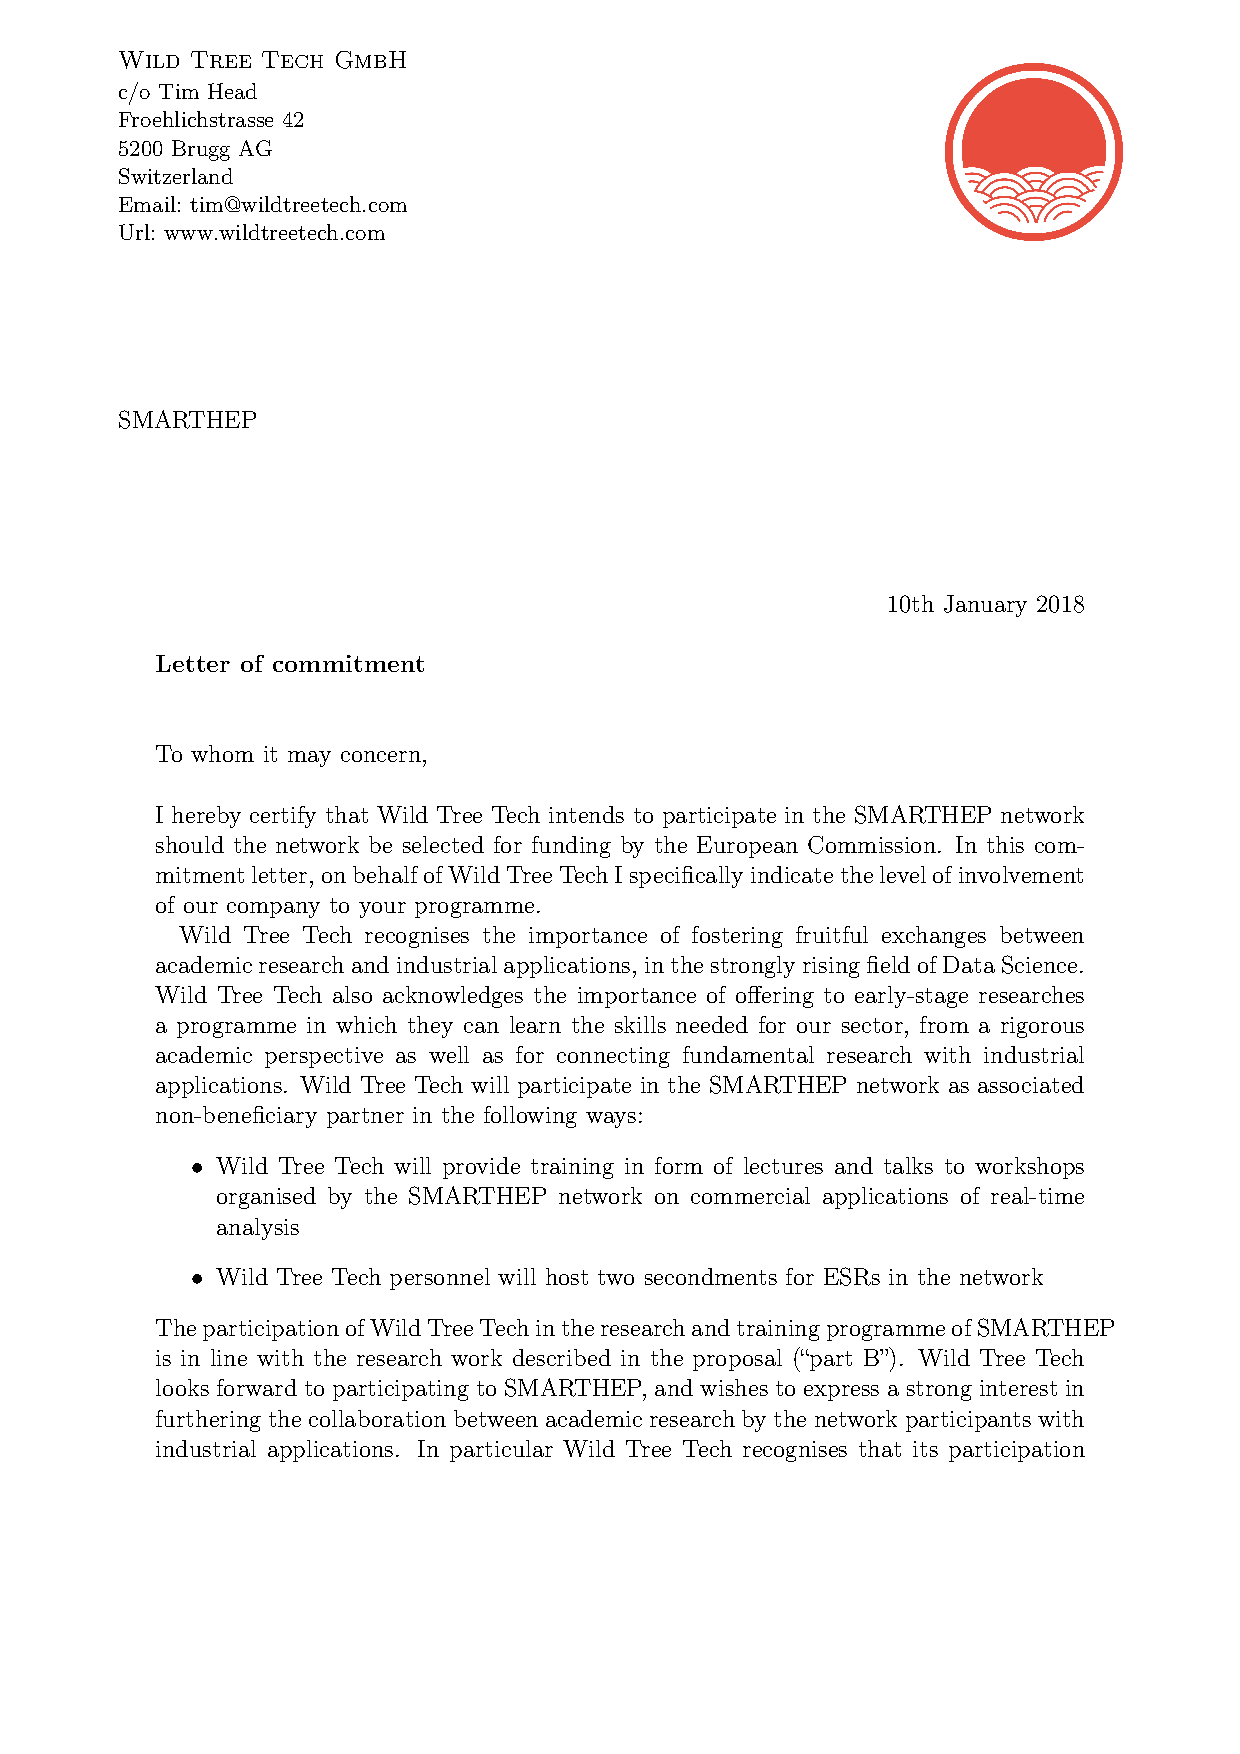
\includepdf[pages={1,2}]{LOC/WTT}
%
\includepdf[pages={1}]{LOC/USC}
%
\includepdf[pages={1}]{LOC/INFN}
%
\includepdf[pages={1}]{LOC/OSU}
%
\includepdf[pages={1,2}]{LOC/Oregon}
%
\includepdf[pages={1}]{LOC/Cincinnati}
%
\includepdf[pages={1,2}]{LOC/VU}
%
\includepdf[pages={1}]{LOC/Radboud}
%
\includepdf[pages={1}]{LOC/HIMT_CommitmentLetter}
%
%%
%%%Please use this section to insert scanned copies of the required Letters of
%%%Commitment from partner organisations.
%%%\thispagestyle{empty}
%

\clearpage
\section*{SEALS OF EXCELLENCE}


\includepdf[pages={1}]{LOC/Ximantis_Seal_Of_Excellence}

\begin{center}

\mbox{ }\\[1ex
\vspace{1cm}]

{\LARGE\bf ENDPAGE}

\vspace{2.5cm}


{\LARGE MARIE SK\L ODOWSKA-CURIE ACTIONS}\\[2ex]

\vspace{2cm}

{\LARGE\bf Innovative Training Networks (ITN)\\
Call: H2020-MSCA-ITN-2017}\\[2ex]

\vspace{3.cm}

{\LARGE PART B}

\vspace{2.5cm}

{\LARGE ``\acronym'' }

\vspace{2.5cm}
 
{\large\bf This proposal is to be evaluated as:}\\
{\large\bf ETN}

\vspace{2.cm}

\end{center}

\end{document}


%\label{LastPage}

